%&preformat-disser
\RequirePackage[l2tabu,orthodox]{nag} % Раскомментировав, можно в логе получать рекомендации относительно правильного использования пакетов и предупреждения об устаревших и нерекомендуемых пакетах
% Формат А4, 14pt (ГОСТ Р 7.0.11-2011, 5.3.6)
\documentclass[a4paper,14pt,oneside,openany]{memoir}

\input{common/setup}            % общие настройки шаблона
\input{common/packages}         % Пакеты общие для диссертации и автореферата
\synopsisfalse                      % Этот документ --- не автореферат
\input{semestr_report/dispackages}    % Пакеты для диссертации
\input{semestr_report/userpackages}   % Пакеты для специфических пользовательских задач

\input{semestr_report/setup}      % Упрощённые настройки шаблона

\input{common/newnames}         % Новые переменные, для всего проекта

%%% Основные сведения %%%
\newcommand{\thesisAuthorLastName}{Гусев}
\newcommand{\thesisAuthorOtherNames}{Владислав Евгеньевич}
\newcommand{\thesisAuthorInitials}{В.\,Е.}
\newcommand{\thesisAuthor}             % Диссертация, ФИО автора
{%
    \texorpdfstring{% \texorpdfstring takes two arguments and uses the first for (La)TeX and the second for pdf
        \thesisAuthorLastName~\thesisAuthorOtherNames% так будет отображаться на титульном листе или в тексте, где будет использоваться переменная
    }{%
        \thesisAuthorLastName, \thesisAuthorOtherNames% эта запись для свойств pdf-файла. В таком виде, если pdf будет обработан программами для сбора библиографических сведений, будет правильно представлена фамилия.
    }
}
\newcommand{\thesisAuthorShort}        % Диссертация, ФИО автора инициалами
{\thesisAuthorInitials~\thesisAuthorLastName}
\newcommand{\thesisUdk}                % Диссертация, УДК
{\todo{000.000}}
\newcommand{\thesisTitle}              % Диссертация, название
{Каскадные схемы для обогащения регенерированного урана при его многократном рецикле в топливных циклах перспективных энергетических реакторов}
\newcommand{\thesisSpecialtyNumber}    % Диссертация, специальность, номер
{01.04.14}
\newcommand{\thesisSpecialtyTitle}     % Диссертация, специальность, название (название взято с сайта ВАК для примера)
{Теплофизика и теоретическая теплотехника}
%% \newcommand{\thesisSpecialtyTwoNumber} % Диссертация, вторая специальность, номер
%% {\todo{XX.XX.XX}}
%% \newcommand{\thesisSpecialtyTwoTitle}  % Диссертация, вторая специальность, название
%% {\todo{Теория и~методика физического воспитания, спортивной тренировки,
%% оздоровительной и~адаптивной физической культуры}}
\newcommand{\thesisDegree}             % Диссертация, ученая степень
{кандидата технических наук}
\newcommand{\thesisDegreeShort}        % Диссертация, ученая степень, краткая запись
{канд. техн. наук}
\newcommand{\thesisCity}               % Диссертация, город написания диссертации
{Москва}
\newcommand{\thesisYear}               % Диссертация, год написания диссертации
{2024}
\newcommand{\thesisOrganization}       % Диссертация, организация
{МИНИСТЕРСТВО НАУКИ И ВЫСШЕГО ОБРАЗОВАНИЯ РОССИЙСКОЙ ФЕДЕРАЦИИ\\
Федеральное государственное автономное образовательное учреждение высшего
образования\\
\textbf {<<Национальный исследовательский ядерный университет <<МИФИ>>\\(НИЯУ МИФИ)}}
\newcommand{\thesisOrganizationShort}  % Диссертация, краткое название организации для доклада
{\todo{НазУчДисРаб}}

\newcommand{\thesisInOrganization}     % Диссертация, организация в предложном падеже: Работа выполнена в ...
{Национальном исследовательском ядерном университете «МИФИ» (НИЯУ МИФИ)}

%% \newcommand{\supervisorDead}{}           % Рисовать рамку вокруг фамилии
\newcommand{\supervisorFio}              % Научный руководитель, ФИО
{Сулаберидзе Георгий Анатольевич}
\newcommand{\supervisorRegalia}          % Научный руководитель, регалии
{кандидат физико-математических наук, доцент}
\newcommand{\supervisorFioShort}         % Научный руководитель, ФИО
{Г.\,А.~Сулаберидзе}
\newcommand{\supervisorRegaliaShort}     % Научный руководитель, регалии
{к.ф.-м.н, доцент}


\newcommand{\consultOneFio}           % Второй научный руководитель, ФИО
{Смирнов Андрей Юрьевич}
\newcommand{\consultOneRegalia}       % Второй научный руководитель, регалии
{кандидат физико-математических наук}
\newcommand{\consultOneFioShort}      % Второй научный руководитель, ФИО
{А.\,Ю.~Смирнов}
\newcommand{\consultOneRegaliaShort}  % Второй научный руководитель, регалии
{к.ф.-м.н}

\newcommand{\consultTwoFio}           % Второй научный руководитель, ФИО
{Невиница Владимир Анатольевич}
\newcommand{\consultTwoRegalia}       % Второй научный руководитель, регалии
{кандидат технических наук}
\newcommand{\consultTwoFioShort}      % Второй научный руководитель, ФИО
{В.\,А.~Невиница}
\newcommand{\consultTwoRegaliaShort}  % Второй научный руководитель, регалии
{к.т.н}

\newcommand{\opponentOneFio}           % Оппонент 1, ФИО
{Палкин Валерий Анатольевич}
\newcommand{\opponentOneRegalia}       % Оппонент 1, регалии
{доктор технических наук}
\newcommand{\opponentOneJobPlace}      % Оппонент 1, место работы
{УРФУ}
\newcommand{\opponentOneJobPost}       % Оппонент 1, должность
{профессор}

\newcommand{\opponentTwoFio}           % Оппонент 2, ФИО
{Алексей Алексеевич Орлов}
\newcommand{\opponentTwoRegalia}       % Оппонент 2, регалии
{доктор технических наук}
\newcommand{\opponentTwoJobPlace}      % Оппонент 2, место работы
{Отделение ядерно-топливного цикла ТПУ}
\newcommand{\opponentTwoJobPost}       % Оппонент 2, должность
{профессор}

%% \newcommand{\opponentThreeFio}         % Оппонент 3, ФИО
%% {\todo{Фамилия Имя Отчество}}
%% \newcommand{\opponentThreeRegalia}     % Оппонент 3, регалии
%% {\todo{кандидат физико-математических наук}}
%% \newcommand{\opponentThreeJobPlace}    % Оппонент 3, место работы
%% {\todo{Основное место работы c длинным длинным длинным длинным названием}}
%% \newcommand{\opponentThreeJobPost}     % Оппонент 3, должность
%% {\todo{старший научный сотрудник}}

\newcommand{\leadingOrganizationTitle} % Ведущая организация, дополнительные строки. Удалить, чтобы не отображать в автореферате
{\todo{Федеральное государственное бюджетное образовательное учреждение высшего
 образования -.-.-.-.-.-.-.-.-.-.-.--.-.-.-.-.-.-.-.-.-.-.-.--..--..-}}

\newcommand{\defenseDate}              % Защита, дата
{\todo{10 июня 2024~г.~в~13 часов}}
\newcommand{\defenseCouncilNumber}     % Защита, номер диссертационного совета
{{МИФИ.2.02}}
\newcommand{\defenseCouncilTitle}      % Защита, учреждение диссертационного совета
{{НИЯУ МИФИ}}
\newcommand{\defenseCouncilAddress}    % Защита, адрес учреждение диссертационного совета
{{Москва, Каширское шоссе, 31}}
\newcommand{\defenseCouncilPhone}      % Телефон для справок
{\todo{+7~(0000)~00-00-00}}

\newcommand{\defenseSecretaryFio}      % Секретарь диссертационного совета, ФИО
{{Куликов Е.Г.}}
\newcommand{\defenseSecretaryRegalia}  % Секретарь диссертационного совета, регалии
{{к.т.н.}}            % Для сокращений есть ГОСТы, например: ГОСТ Р 7.0.12-2011 + http://base.garant.ru/179724/#block_30000

\newcommand{\synopsisLibrary}          % Автореферат, название библиотеки
{\todo{Название библиотеки}}
\newcommand{\synopsisDate}             % Автореферат, дата рассылки
{\todo{DD mmmmmmmm YYYY года}}

% To avoid conflict with beamer class use \providecommand
\providecommand{\keywords}%            % Ключевые слова для метаданных PDF диссертации и автореферата
{}
             % Основные сведения
\input{common/fonts}            % Определение шрифтов (частичное)
\input{common/styles}           % Стили общие для диссертации и автореферата
\input{semestr_report/disstyles}  % Стили для диссертации
\input{semestr_report/userstyles} % Стили для специфических пользовательских задач

%%% Библиография. Выбор движка для реализации %%%
% Здесь только проверка установленного ключа. Сама настройка выбора движка
% размещена в common/setup.tex
\ifnumequal{\value{bibliosel}}{0}{%
    \input{biblio/predefined}   % Встроенная реализация с загрузкой файла через движок bibtex8
}{
    \input{biblio/biblatex}     % Реализация пакетом biblatex через движок biber
}

% Вывести информацию о выбранных опциях в лог сборки
\typeout{Selected options:}
\typeout{Draft mode: \arabic{draft}}
\typeout{Font: \arabic{fontfamily}}
\typeout{AltFont: \arabic{usealtfont}}
\typeout{Bibliography backend: \arabic{bibliosel}}
\typeout{Precompile images: \arabic{imgprecompile}}
% Вывести информацию о версиях используемых библиотек в лог сборки
\listfiles

\begin{document}

\input{common/renames}                 % Переопределение именований

% Титульный лист (ГОСТ Р 7.0.11-2001, 5.1)
\thispagestyle{empty}
\begin{center}
\thesisOrganization
\end{center}
%
\vspace{0pt plus4fill} %число перед fill = кратность относительно некоторого расстояния fill, кусками которого заполнены пустые места
\begin{center}
\textbf {\large Методические...}
\end{center}
%
\begin{center}
{\large %\MakeUppercase
\thesisTitle}

\vspace{0pt plus2fill} %число перед fill = кратность относительно некоторого расстояния fill, кусками которого заполнены пустые места
\begin{minipage}[b]{0.5\linewidth}
    \begin{flushright}
        Научная специальность \thesisSpecialtyNumber\ "---
        <<\thesisSpecialtyTitle>>
    \end{flushright}
  \end{minipage}

\vspace{0pt plus2fill} %число перед fill = кратность относительно некоторого расстояния fill, кусками которого заполнены пустые места
\end{center}


\hfill
Каскады
           % Титульный лист

\include{semestr_report/contents}        % Оглавление
\ifnumequal{\value{contnumfig}}{1}{}{\counterwithout{figure}{chapter}}
\ifnumequal{\value{contnumtab}}{1}{}{\counterwithout{table}{chapter}}
\chapter*{Введение}                         % Заголовок
\addcontentsline{toc}{chapter}{Введение}    % Добавляем его в оглавление


\section{Востребованность изотопных смесей (бинарных и многокомпонентных) в различных областях науки и техники (примеры).}
Востребованность изотопных смесей (бинарных и многокомпонентных) в различных областях науки и техники (примеры).


\section{Принципы каскадирование одиночных разделительных элементов. Роль теории каскадов для разделения изотопных смесей при изучении физических закономерностей массопереноса компонентов в подобных установках.}

Принципы каскадирование одиночных разделительных элементов. Роль теории каскадов для разделения изотопных смесей при изучении физических закономерностей массопереноса компонентов в подобных установках.


\section{Понятие и роль модельных каскадов в общей теории.}

Понятие и роль модельных каскадов в общей теории.
    % Введение
\ifnumequal{\value{contnumfig}}{1}{\counterwithout{figure}{chapter}
}{\counterwithin{figure}{chapter}}
\ifnumequal{\value{contnumtab}}{1}{\counterwithout{table}{chapter}
}{\counterwithin{table}{chapter}}

\chapter{Анализ литературы, патентов и обзор практики рецикла урана}\label{ch:ch1}

\section{Теоретические основы}

\subsection{Основы теории разделения в каскадах}
\textcolor{red}{Базовые понятия (разделительный элемент, симметричн.-противоточное соединений, каскад) + основные уравнения (балансы, срез, коэффициенты разделения ступеней)}

\dots

\subsection{Модельные каскады}

Тогда как обогащение природного урана можно свести к простой задаче разделения бинарной смеси, обогащение переработанного урана является задачей разделения изотопов многокомпонентной изотопной смеси.
% А сложность расчетов молекулярно-селективного переноса для многокомпонентных изотопных составов заключается в необходимости использования математических моделей для разделения многокомпонентных изотопных смесей (хотя это касается и разделения неурановых химических элементов, например вольфрама).

\subsubsection{Модель симметрично-противоточного каскада}

Модели, которые будут рассмотрены в данном разделе -- «квазиидеальный» каскад, R-каскад, поступенный расчет -- вытекают из модели симметрично-противоточной коммутации ступеней каскада.

\dots

Вычислительные эксперименты, проводимые с целью исследования каскадов, опираются на использование специальных математических моделей, которые будут представлены в текущем разделе. Они позволяют заметно упростить изучение закономерностей изотопно-селективного массопереноса в разделительных каскадах. Этот вспомогательный инструмент принято называть модельным каскадом.

Физико-математические модели каскадов основанны на фундаментальных законах, таких как закон сохранения вещества.
Эти теоретические описания адекватны процессу разделения в реальных каскадах, состоящих из тысяч разделительных аппаратов.
В качестве разделительных аппаратов сегодня, как правило, используются газовые центрифуги.

В области математического моделирования разделительных каскадов на сегодня разработан обширный набор расчетных моделей, которые могут быть применены в том числе и к задаче обогащения регенерированного урана.
В нашем случае для моделирования физического процесса разделения изотопов урановой смеси может быть применен ряд специальных математических моделей.

Наиболее общая из таких моделей называется «квазиидеальным» каскадом, где предполагается постоянство относительных коэффициентов разделения, а также срезов парциальных компонентов по каскадным ступеням \cite{yamamotoMulticomponentIsotopeSeparating1978}.
В настоящее время он используется в двух приближениях: со слабым обогащением (Q-каскад \cite{borisevichNewApproachOptimize2011, kolokoltsovDesignCascadesSeparating1970, zengQCascadeExplanation2012}) и произвольным обогащением (квазиидеальный каскад \cite{sulaberidzeSpecialFeaturesEnrichment2006}).
Применение модельных каскадов значительно упрощает как анализ закономерностей массообмена в каскаде для многокомпонентного разделения, так и соответствующий расчет.
В исследованиях, как правило, когда обогащенный переработанный уран обогащается многопоточными схемами, часто используется модель R-каскада (Matched Abundance Ratio Cascade-MARC \cite{delagarzaMulticomponentIsotopeSeparation1961, woodEffectsSeparationProcesses2008, kazukihidaSimultaneousEvaluationEffects1986}).
Это особый случай `квазиидеального' каскада. Здесь условие отсутствия смешивания выполняется для выбранной пары компонентов (например, это могут быть изотопы $^{235}$U и $^{238}$U).
Еще раз подчеркнем, что все вышеупомянутые каскадные модели действуют как физически эквивалентные представления и, как показано в \cite{sulaberidzeClassificationModelCascades2020}, могут быть выведены из <<обобщенного модельного каскада>>, которым является симметрично-противоточный каскад с постоянными по его длине относительными коэффициентами разделения).




\subsubsection{Модель «квазиидеального» каскада}
\dots

\subsubsection{Каскад с несмешиванием относительных концентраций двух заданных компонентов смеси (R-каскад)}
\dots

\subsubsection{Поступенный расчет}

Стоит упомянуть, что существует альтернативный подход к каскадному расчету, когда набор из шести уравнений включает 10 основных внутренних параметров:

$L_{i}, C_{i}, L_{i}^{\prime}, C_{i}^{\prime}, L_{i}^{\prime \prime}, C_{i}^{\prime \prime}, q_{i}, \theta_{i}, N_{i}, l_{i}$,

где $L_{i}, L_{i}^{\prime}, L_{i}^{\prime \prime}$ и $C_{i}, C_{i}^{\prime}, C_{i}^{\prime \prime}$ -- 
это потоки питания, продукта и отвала и их концентрации соответственно; $q_{i}$ -- коэффициент разделения; $\theta$ -- коэффициент деления потока на ступени (срез); $N_{i}$ -- число ступеней; и $l_{i}$ -- поток питания отдельной центрифуги.

Эти параметры связаны шестью уравнениями:
$\begin{array}{c}
  {L_{i}^{\prime}+L_{i}^{\prime \prime}=L_{i}} \\
  {L_{i}^{\prime} C_{i}^{\prime}+L_{i}^{\prime \prime} C_{i}^{\prime \prime}=L_{i} C_{i}} \\
  {q_{i}=\frac{(1-C_{i}^{\prime \prime}) C_{i}^{\prime}}{(1-C_{i}^{\prime}) C_{i}^{\prime \prime}}} \\
  {q_{i}=q_{i}\left(l_{i}, \theta_{i}\right)} \\
  {\theta_{i}=\frac{L_{i}^{\prime}}{L_{i}}} \\
  {l_{i}=\frac{L_{i}}{N_{i}}}
\end{array}$

Помимо этих 6$n$ соотношений, описывающих отдельные ступени, необходимо учитывать уравнение, связывающее межкаскадные потоки -- балансные уравнения, вид которых зависит от рассматриваемой схемы коммутации ступеней. Для каскада, показанного на рис. 1, эти уравнения записаны в виде:

$\begin{array}{c}
  {L_{1}=L_{2}^{\prime \prime}, \ldots ; L_{i}=L_{i-2}^{\prime}+L_{i+1}^{\prime \prime}, \ldots ;} \\
  {L_{1} C_{1}=L_{2}^{\prime \prime} C_{2}^{\prime \prime}, \ldots ; L_{i} C_{i}=L_{i-2}^{\prime} C_{i-2}^{\prime}+L_{i+1}^{\prime \prime} C_{i+1}^{\prime \prime}, \ldots}
\end{array}$

В дополнение к этим соотношениям необходимо учитывать граничные условия, относящиеся к внешним и внутренним параметрам. Например для симметричного противоточного каскада, они выражаются соотношениями: 
$P=L_{n}^{\prime} ; C_{P}=C_{n}^{\prime} ; W=L_{1}^{\prime \prime} ; C_{W}=C_{1}^{\prime \prime}$

, которые выполняются для каждой ступени каскада \cite{palkinDeterminationOptimalParameters2012}. Эти уравнения описывают отношения между соседними ступенями и, опираясь на ряд граничных условий, могут служить эффективной репрезентацией каскада. 


Работе по поиску схем для обогащения регенерата предшествовали разработки математического аппарата для моделирования разделения многокомпонентных смесей \cite{delagarzaMulticomponentIsotopeSeparation1961}.
Изначально, эта идея рассматривалась для газодиффузионного метода разделения, которая в последующем была адаптирована для метода газовой центрифуги с характерным б'ольшим коэффициентом разделения \cite{yamamotoMulticomponentIsotopeSeparating1978}.
Проходя через основные вехи развития модельных каскадов для моделирования многокомпонентных изотопных смесей, в работе \cite{delagarzaMulticomponentIsotopeSeparation1961} предложена модель R-каскада, а в \cite{levin1963} -- М*-каскада.
Затем в \cite{kolokoltsovDesignCascadesSeparating1970} разработана модель Q-каскада, а в \cite{sazykinKvaziidealnyeKaskadyDlya2000} -- квазиидеального.

\subsection{Истоки возникновения проблемы с $^{232,234,236}$U}

В конечном товарном продукте -- низкообогащенном уране -- регламентировано содержание изотопов четного ряда -- $^{232,234,236}$U.
Наличие строгих ограничений обсуловлено нейтронно-физическими и радиационными свойствами четных изотопов $^{232,234,236}$U \cite{smirnovEvolutionIsotopicComposition2012, proselkovAnalizVozmozhnostiIspolzovaniya2003, dudnikovInfluence236UEfficacy2016}.
Эти изотопы, возникшие при облучении топлива и в ходе последующего его хранения, не могут быть извлечены в ходе переработки из урановой смеси. Они могут быть удалены только с использованием технологий разделения изотопов, что и затрудняет обогащение регенерированного урана для его возврата в ЯТЦ.

Так, первый в этом ряду изотоп $^{232}$U является родоначальником длинной цепочки распада, в которую входят нуклиды-излучатели жёстких гамма-квантов.
Основным дочерним источником интенсивного гамма-излучения (2.6 МэВ) является короткоживущий $^{208}$Tl ($t_{\frac{1}{2}}=3.65$ мин.) \cite{matveevUran232EgoVliyanie1985,abbasProliferationResistanceFeatures2013}. Опасность на производстве также представляет еще один дочерний изотоп -- $^{220}$Rn (торон) вследствие его эманирования в воздух рабочей зоны.

$^{232}$U вместе $^{234}$U превносят альфа-частицы в смесь гексафторида урана ($UF_6$ -- соединение, используемое в процессе обогащения урана \cite{orlovWayObtainUranium2015, orlovDesublimationPurificationTransporting2017}), вероятно, приводя к его диссоциации, что может привести к нежелательному появлению и дальнейшему осаждению в каскаде легких компоненты, таких как, например свободный фтор ($F_2$) \cite{kryuchkovObogashchennyyUranDobavleniem2007, bernhardtRadiationEffectsAlpha1958, shmelevRazrabotkaRaschetnoyModeli2012}.

$^{236}$U, являясь паразитным поглотителем нейтронов, препятствует развитию цепной реакции.
Этот эффект отравления реактора должен быть скомпенсирован дополнительным количеством делящегося $^{235}$U в топливе.
То есть, для обеспечения требуемого эквивалента уровня обогащения по $^{235}$U, к заданной концентрации $^{235}$U в продукте для случая обогащения природного урана необходимо обеспечить добавку делящегося $^{235}$U.
Ее величина определяется наличием $^{236}$U:
$C_{235 экв.}^{P}=C_{235 прир.}^{P}+\Delta C_{235}$, где $\Delta C_{235}$ соответствует некоторой функции $f\left(C_{236}^{P}\right)$, которая в простейшем случае является линейной вида $K_{236} \times C_{236}^{P}$. $K_{236}$ называют коэффициентом компенсации реактивности. Его значение значение в зависимости от (типа реактора и топливной кампании?) может лежать в пределах 0.2--0.6 \cite{delagarzaMulticomponentIsotopeSeparation1961, delculAnalysisReuseUranium2009}. 

$^{234}$U имеет тенденцию захватывать нейтрон и превращаться в делящийся $^{235}$U, что должно уменьшить необходимую компенсацию $^{236}$U \cite{dyachenkoIspolzovanieRegenerirovannogoUrana2012}, что в расчетах не учитывается ввиду порядка малости.

Содержание этих изотопов в низкообогащенном продукте может регулироваться различными стандартами, такими как, например, ASTM C996 - 15 \cite{c26committeeSpecificationUraniumHexafluoride}.

\subsection{Задача обогащения регенерированного урана с точки зрения разделительных технологий}

Специфика задачи обогащения регенерированного урана заключается в том, что она представляет собой более сложную разделительную проблему.
Это обусловлено тем, что, в отличие от случая обогащения природного урана, регенерированный уран представляет собой многокомпонентную смесь и, помимо обогащения целевого изотопа -- $^{235}$U, необходимо одновременно выполнять ограничения на еще три изотопа -- $^{232}$U, $^{234}$U и $^{235}$U.
Таким образом, при решении задачи обогащения регенерата необходимо обеспечить:
\begin{enumerate}
  \item Соответствие произведенного низкообогащенного урана необходимым требованиям (спецификациям), которое может быть сформулировано как удовлетворение ограничения на присутствие нежелательных "четных" изотопов урана. Так, в соответствии с распространенными стандартами для низкообогащенного урана:
  \begin{enumerate}
    \item концентрация изотопа $^{232}$U в низкообогащенном уране строго ограничена величиной $5\cdot10^{-7}$\%, или, в некоторый случаях, $2\cdot10^{-7}$\% \cite{smirnovKaskadnyeShemyZadachah2012}.
    \item Отношение концентраций изотопов $^{234}$U и $^{235}$U в продукте не должно превышать 0.02.
    \item $^{236}$U должен быть скомпенсировано дополнительным количеством делящегося $^{235}$U в низкообогащенном уране.
  \end{enumerate}
  \item Использование восстановленного урана на единицу продукта НОУ в необходимой пропорции ($\approx$0.93), что соответствует возврату в топливный цикл в виде 1 кг свежего топлива 1 кг ОЯТ. Такое условие может быть связано с мерами контроля оборота делящихся материалов, что особенно актуально для экспорта ядерного топлива. Величина  $\approx$0.93 соответствует доле извлекаемой в ходе переработки ОЯТ урановой фракции.
  \item Вовлечение в топливный цикл максимально возможной доли изотопа $^{235}$U для повышения экономии природного урана
\end{enumerate}

Также могут иметь место следующие условия:
\begin{enumerate}
  \item Вывод из топливного цикла изотопов $^{232,234,236}$U, который можно обеспечить только посредством изотопного разделения. Концентрации этих нежелательных искусственных изотопов должны быть минимизированы в условиях многократной переработки урановой составляющей топлива. Это важно чтобы избежать их накопления к последующим рециклам.
  \item Предотвращение нежелательных потерь работы разделения в ходе операции разделения изотопов. Такие потери могут быть связаны с недостатками каскадных схем, когда осуществляется смешение изотопных составов с различными концентрациями $^{235}$U. 
  \item Избежание накопления нештатных (высокотоксичных) отходов -- побочных продуктов с высокой концентрацией изотопов $^{232,234}$U. К тому же, в них теряется $^{235}$U.
  \item Предел допустимой концентрации $^{235}$U на любом из стадий производства может быть ограничен лицензией обогатительного комбината.
  \item Предел доступных для решения задачи разделительных мощностей.
  \item Ограничения на расход сырья разбавителя, которым может быть как природный уран, так и обедненный или предварительно подготовленный НОУ.
\end{enumerate}

Политика вовлечения регенерированного урана в ЯТЦ позволяет достигать экономии природного урана на уровне 11--20\% и многократного снижения объемов высокоактивных радиоактивных отходов за счет переработки ОЯТ \cite{delculAnalysisReuseUranium2009}. Возможность же осуществлять многократный рецикл урана и курс на удлинение (пролонгацию) топливных кампаний, связанный с повышением исходного уровня обогащения, открывает перспективы еще б`ольших преимуществ повторного использования делящегося материала.
Все это делает актуальным разработки каскадных обогатительных схем, позволяющих эффективно использовать регенерированный уран при производстве товарного НОУ с учетом всех описанных выше требований и ограничений как в условиях однократного, так и многократного рецикла урана.


\section{Промышленный опыт}\label{sec:ch1/sec1}
Промышленный опыт замыкания ЯТЦ опирается на технологии переработки ОЯТ и последующего рецикла ядерных материалов.
В России имеется уникальный технологический задел, связанный с переработкой ОЯТ \cite{balihinSostoyaniiPerspektivahRazvitiya2018}.
Таким образом, заключительная часть ЯТЦ (back-end) является перспективным направлением развития международного бизнеса Росатома \cite{efimenkoProblemyPerspektivyRazvitiya2017}. 

Что касается рецикла ядерного топлива, зарубежный опыт исторически базируется на однократном использовании MOX-топлива.
В данной работе будем опираться на Российский опыт возврата топлива в ЯТЦ \cite{international2003iaea}.
К тому же, по части повторного использования урановой составляющей, отечественную ядерную индустрию можно считать глобальным лидером.
Эта практика вовлечения регенерата урана в топливные циклы энергетических реакторов базируется на смешении регенератов урана, извлекаемых из ОЯТ ВВЭР и ОЯТ транспортных реакторов с высоким содержанием $^{235}$U.
Такая схема реализована для производства исходного сырья для изготовления топлива РБМК на заводе РТ-1 \cite{volkVozvratUranaIz2010}.
Более того, этот вариант также апробирован для изготовления опытных ТВС для реакторов ВВЭР \cite{proselkovAnalizVozmozhnostiIspolzovaniya2003}, требующих более высокого уровня обогащения.

На сегодняшний день для широкомасштабного использования регенерированного урана существует ряд препятствий, состоящих в ограничениях мощностей переработки ОЯТ, ограниченном опыте промышленной эксплуатации топлива на основе обогащенного регенерата, неготовности фарбрикационного, радиохимического и сублиматного производств вводить производственные линии для материала с повышенной радиотоксичностью (отсутствие у последних двух лицений на работу с материалом >1\% $^{235}$U), а также неисследованный вопрос хранения ОГФУ с $^{232,234}$U.

При этом, опираясь на передовой уровень разделительной технологии \textcolor{red}{не встречал работы о пригодности ГЦ к обогащению регенерата}, можно заключить, что задача обогащения регенерата до необходимого для повторного использования в энергетических ядерных реакторах уровня концентрации изотопа $^{235}$U может быть решена.
Сложившаяся к текущему моменту научно-производственная база и лидирующие объемы имеющихся в нашей стране промышленных разделительных мощностей, основанных на центробежном методе разделения, являются основным аргументом в пользу готовности к вовлечению регенерата в топливный цикл легководных реакторов.
Однако, ввиду долгосрочных планов отрасли по замыканию ЯТЦ и развитию международных топливных поставок, необходимо предполагать необходимость  многократного рецикла и наличие дополнительных ограничений на расход материалов.


\section{Задача поиска оптимальной схемы}

Перейдем к вопросу подбора каскадной схемы для производства НОУ, способной обеспечить наилучшее решение с точки зрения выбранных критериев.
Такими критериями  обычно выступают показатели, называемые интегральными в теории разделения изотопов: расход природного урана и затраты работы разделения.
Они подлежат минимизации, однако зачастую являются конкурирующими.
В качестве целевой функции можно рассматривать аддитивный критерий стоимости или энергозатрат, который может включать в себя, помимо расхода природного урана и затрат работы разделения, расходы (стоимостные или энергетические) на утилизацию нештатных отходов, а также на прочие вовлекаемые (в качестве потоков питания) материалы, например ОГФУ, для которого такой показатель может быть отрицательным.

Следует напомнить, что задача при этом должна быть решена в рамках набора заданных условий, а это накладывает ограничения на оптимизацию целевых показателей.
К тому, же могут возникнуть дополнительные факторы, которые могут претендовать на роль первостепенных показателей эффективности.
Ими могут быть минимум нештатного отхода, минимизация загрязнения резделительного оборудования.

\section{Расчетная модель}

В данной работе будут использованы математические модели "квазиидеального" каскада и его частный случай -- R-каскад. Расчеты будут проведены в предположениях симметрично-противоточной схемы коммутации, а также при одинаковом коэффициенте разделения $q$ на каждой ступени.

\section{Сравнительный анализ известных схем}

История теоретических исследований вопроса повторного использования урана в ядерном топливе насчитывает около полувека.
В этом разделе будет рассмотрена эволюция методик, предложенных для решения задачи обогащения регенерированного урана с целью его возврата в топливный цикл энергетических реакторов.
Развитие подходов к вовлечению регенерата в производство низкообогащенного урана можно проследить через историю совершенствования предлагаемых каскадных схем.
Для каждой рассмотренной схемы будет проведен критический анализ, выявляющий ее достоинства и недостатки.

\subsection{Основные модификации ординарного каскада}

Непосредственное применение простейшей схемы -- ординарного каскада, используемого для обогащения природного урана имеет существенные ограничения в рамках поставленной нами задачи.
В условиях многократного рецикла, она не позволяет добиться желаемого результата, ввиду наличия ограничений на присутствие в конечном продукте -- низкообогащенном уране -- четных изотопов.
Такое ограничение и подтолкнуло исследователей к развитию подходов к производству НОУ из обогащенного регенерата с учетом заданных требований.
В работах \cite{sulaberidzeNekotoryhRazdelitelnyhProblemah2004,sulaberidzeProblemsRefinementRecycled4, smirnovKaskadnyeShemyZadachah2012} было показано, что отрицательное влияние указанных изотопов делает непригодным для обогащения регенерата ординарный каскад (каскад, имеющий три внешних потока – питание, отбор и отвал), используемый для обогащения природного урана. Это происходит, поскольку при обогащении регенерата по $^{235}$U в таком каскаде, в отборе, помимо $^{235}$U неминуемо будут концентрироваться все легкие компоненты, в первую очередь $^{232}$U. Поэтому ординарный каскад применим только для обогащения относительно «чистого» состава регенерата, в котором содержание $^{232}$U меньше допустимой нормы на порядок и более, что нехарактерно для большинства изотопных составов выгружаемого из активной зоны ВВЭР облученного топлива \cite{bormanTehnikoekonomicheskiyAnalizVozmozhnyh2012}.

Рассмотрим же технические решения, позволяющие корректно (соблюдая вышеозначенные условия) решить задачу обогащение регенерата. Начнем с ряда схем, основанных на ординарном (трехпоточном) каскаде.
Его можно применять, например, следующими способами (рис. \ref{fig:diagram1}) \cite{smirnovKaskadnyeShemyZadachah2012}:
\begin{enumerate}
  \item Добавление смеси регенерированного урана к природному урану перед подачей в каскад рис. (рис. \ref{fig:diagram1}.1 ).
  \item Получение обогащенной фракции из регенерата и последующее ее разбавление природной урановой смесью (рис. \ref{fig:diagram1}.2 ).
  \item Подготовка смеси НОУ из природного урана немного больше, чем необходимо для получения товарного НОУ требуемого качества, с последующим разбавлением его регенератом (рис. \ref{fig:diagram1}.3 ).
\end{enumerate}

\begin{figure}[ht]
  \centerfloat{\includegraphics[scale=0.7]{cascades/diagram1}}
  \caption{Схемы на основе ординарного каскада}\label{fig:diagram1}
\end{figure}

Для всех вариантов схем рис. \ref{fig:diagram1} сотношение между расходом регенерата и разбавителем природного происхождения определяется пределом допустимой концентрации $^{232}$U в конечном продукте -- низкообогащенном уране. Также делается поправка на необходимость компенсации отрицательной реактивности $^{236}$U. В то же время концентрация $^{235}$U не должна быть ниже, чем требуется для НОУ с определенными свойствами.

Основным преимуществом таких схем является простота реализации, поскольку нет необходимости в модификации устройства каскада -- операции разбавления осуществляются за пределами  ординарного каскада.
При этом, как недостаток можно выделить потери работы разделения, возникающие из-за смешения потоков с различными изотопными концентрациями $^{235}$U.
Также эти схемы не могут обеспечить полный возврат ОЯТ в ЯТЦ.
Однако такие схемы не пригодны для решения задачи вовлечения регенерата в условияx многократного рецикла, что будет в очередной раз продемонстрировано в данной диссертационной работе.

Рассмотрим вариант схемы, рис.\ref{fig:diagram1}.2, лучшим образом подходящий для задачи возврата регенерата урана второго рецикла (NET).

Схема рисунка \ref{fig:diagram1}.2 представляет собой возможный способ снижения накопления четных изотопов в регенерате урана \cite{SposobIzotopnogoVosstanovleniyaa}. Разбавление осуществляют следующим образом: сначала из регенерата в ординарном каскаде получают высокообогащенный уран (ВОУ), который затем разбавляют смесью, не содержащей минорных изотопов, добиваясь нужного содержания изотопа $^{235}$U в финальном продукте-низкообогащенном уране. Например, таким разбавителем может быть природный уран или отвалы разделительного производства. Для обогащения по изотопу $^{235}$U перед последующим разбавлением предложена массовая концентрация $\approx$36\% \cite{SposobIzotopnogoVosstanovleniyaa}. Практическое использование данной схемы ограничивают следующие недостатки: 
\begin{enumerate}
  \item потери работы разделения при разбавлении ВОУ (количественные оценки величин затрат работы разделения для рассматриваемой схемы будут представлены в разделе ... .
  \item ухудшение радиационной обстановки из-за загрязненности разделительного оборудования примесными изотопами, в частности $^{232}$U, ухудшающим радиационную обстановку.
  \item необходимость обогащения материала до уровня высокообогащенного урана, когда концентрация изотопа $^{235}$U превышает 20\%.
  Такой подход может иметь ограничения со стороны регулятора -- обогатительный комбинат может быть не в праве нарабатывать материал с такой высокой концентрацией $^{235}$U -- ввиду режима нераспространения.
\end{enumerate}

Как будет показано в разделе ..., базовые модификации ординарного каскада не способны решить задачу возврата в ЯТЦ регенерированного урана в условиях многократного рецикла.
Причем это невозможно даже если пренебречь нормативным ограничением на производство ВОУ.
Таким образом, рассмотрение приведенного ряда модификаций ординарного каскада подталкивает к дальнейшим поискам схем, которые бы нивелировали перечисленные недостатки.
Ниже дан критический анализ модификаций каскадных схем для обогащения регенерированного урана, основанных на использовании одиночных каскадов, имеющих дополнительные внешние потоки и двойных каскадов.

\subsection{Каскады с дополнительными внешними потоками (многопоточные схемы)}

Под внешними потоками следует понимать потоки, подаваемые в качестве питания каскада, а под внутренними -- потоки, циркулирующие внутри каскада. 

\subsubsection{Применение дополнительного потока-разбавителя}

Предожена схема с дополнительным потоком питания в виде регенерата, который подают на отдельную ступень рис. \ref{fig:2_inputs}) \cite{sulaberidzeQuasiidealCascadesAdditional2006}.
\begin{figure}[ht]
  \centerfloat{\includegraphics[scale=0.07]{cascades/2in}}
  \caption{Каскад с дополнительным потоком питания}\label{fig:2_inputs}
\end{figure}

Этот метод позволяет избежать потери работы разделения в ходе смешения потоков с различными концентрациями $^{235}$U, располагая дополнительный входной поток там, где концентрации внешнего и внутреннего потоков в $^{235}$U совпадают.
Отсюда, преимущество схемы с дополнительным потоком питания по сравнению с предыдущими обычными схемами, связано с отсутствием потерь работы разделения \cite{smirnovKaskadnyeShemyZadachah2012, sulaberidzeQuasiidealCascadesAdditional2006}.

Однако общим недостатком всех вышеупомянутых схем (рис. \ref{fig:diagram1} и \ref{fig:2_inputs}), является необходимость использования большого количества природного урана.
Вне зависимости от их устройства, для решения поставленной задачи, необходимо осуществлять разбавление регенерата существенным количеством природного урана, в несколько раз превышающим долю используемого регенерата. Это необходимо, прежде всего, чтобы снизить содержание $^{232}$U в продукте.
Тем не менее, при повторном использования топлива ВВЭР, даже такой подход может обеспечить значительную экономию природного урана $\approx$16\% уже на первом рецикле.
Суммарная же экономия природного урана за всю серию рециклов будет складываться из уменьшающихся с каждым рециклом показателей сэкономленного природного сырья. 
Применение же многократного рецикла, позволяет и дальше, используя материалы повторно, частично замещать расход природного ресурса \cite{colemanEvaluationMultipleSelfrecycling2010}), как показано в оценках в \cite{smirnovEvolutionIsotopicComposition2012}.

Проблема необходимости обеспечивать питание каскада преобладающим количеством природного урана , чтобы, в сущности, "разбавлять" четные изотопы  $^{232,234}$U, содержащиеся в регенерате, идет бок о бок с невозможностью обеспечить условие "полного" возврата выгоревшего топлива в ЯТЦ.
Для рассмотренных схем, такое условие, заключающееся в использовании 1 кг ОЯТ на 1 кг НОУ продукта, достижимо только для изотопных составов первого (иногда второго) рецикла топлива легководного реактора.
Таким образом, с помощью такой схемы нельзя обеспечить заданую пропорцию вовлечения регенерированного урана в условиях многократного рецикла \cite{smirnovApplyingEnrichmentCapacities2018}.
На примере рассматриваемого каскада с двумя питаниями, начиная с третьего цикла, расходовать требуемый уровень регенерата становится невозможно из-за ухудшения изотопного состава урана и наличия ограничений на изотопы $^{232,236}$U.

Так, в \cite{smirnovApplyingEnrichmentCapacities2018} были рассчитаны основные показатели, характеризующие экономику разделительного процесса: расход природного урана и затраты работы разделения (РР).
Было показано, что для каждого из первых двух циклах можно достичь экономии природного урана на уровне $\approx$20\%. Затем, этот показатель ухудшается, так как при заданных условиях, к третьему циклу повторного использования происходит значительная деградация изотопного состава.
Чтобы повысить пределы экономии природного урана, необходимо искать альтернативный разбавитель. Например, таким материалом может послужить обедненный уран (так называемые «хвосты» (или отвалы) -- побочный продукт процесса обогащения).
Он может быть эффективно использован для частичной замены природного урана в качестве основного разбавителя.
При этом, обедненный уран (ОГФУ) часто незаслуженно записывается в категорию «отходов», тогда как, благодаря современным технологиям обогащения, этот материал можно использовать как полезный ресурс.
И это, только лишь за счет возможностей обогатительных производств, не говоря о перспективах наработки плутония из ОГФУ в быстрых реакторах.

Для отечественной ядерной индустрии, $^{235}$U из "богатых" источников ОГФУ ($\approx$0.3\%), является важным источником сырья для производства ядерного топлива, а также доходным международным бизнесом \cite{oecdManagementDepletedUranium2001}.
Имеющиеся в мире запасы $\approx$1.2 миллиона тонн <<богатых>> хвостов (0.3\%) дают эквивалент 336 тысяч т. эквивалента природного урана при концентрации U-235 в отвале 0.14\%. Этого достаточно, чтобы обеспечить на 5 лет топливом весь мировой парк энергетических реакторов.
Стоит отметить, что наличие ОГФУ такой категории связано с историей развития обогатительного производства. Ввиду того, что диффузионный метод разделения -- технология первого поколения -- требует колоссальных затрат энергии на единицу РР, получение обогащенного продукта было целесообразней осуществлять с б'ольшими затратами природного урана.
Напомним, что выбор в пользу затрат на каждый из этих показателей связан с компромиссом, определяемым, во многом, экономическими факторами: себестоимостью единицы работы разделения и стоимостью сырья. 
Итак, согласно отчету ГК Росатом 2018 г., поставки из вторичных источников (складские запасы энергокомпаний и некоторых государств, дообогащение обедненного гексафторида урана, регенерированный уран и пр.) оцениваются на уровне 20 тыс. т в эквиваленте природного урана.

Перейдем к описанию каскада, позволяющего задействовать ОГФУ в повторном обогащении регенерированного урана.
Такая схема изображена на рис. \ref{fig:3_inputs}, где $F_{1}, F_{2}, F_{3}$ -- потоки питания в виде ОГФУ, природного урана и регенерата, соответственно; а $W$ и $P$ -- потоки отвала и питания.
Основной принцип устройства данной схемы состоит в том, что входные потоки располагают там, где концентрации внешнего и внутреннего потоков в $^{235}$U совпадают.
Подробное описание математической модели приведено в \cite{smirnovEnrichmentRegeneratedUranium2014}.

\begin{figure}[ht]
  \centerfloat{\includegraphics[scale=0.17]{cascades/3in}}
  \caption{Каскад с тремя потоками питания}\label{fig:3_inputs}
\end{figure}

Основным преимуществом использования каскада рис. \ref{fig:3_inputs} является возможность б'ольшей экономии природного урана.
В \cite{smirnovApplyingEnrichmentCapacities2018}, например, демонстрируется экономия половины природного урана на каждом рецикле.
Однако этот эффект достигается ценой дополнительного расхода РР. При этом возможен выбор соотношения разбавителей и, что позволяет регулировать экономию природного урана и перерасход РР.
Эта особенность позволяет «настраивать» каскад для достижения компромисса между этими показателями, которые являются основными (интегральными) характеристиками разделительного процесса.
Такой прием может позволить добиваться оптимального по себестоимости баланса затрат на эти два конкурирующих показателя.
Заметим, что в качестве критериев для выбора оптимальной схемы как правило и используют минимизацию работы разделения и расхода природного урана для получения единицы товарного НОУ. Эти характеристики являются ключевыми для экономики производства низкообогащенного урана. Иными словами, именно они, в основном, и определяют величину удельных затрат на получение коммерческого продукта.

Кроме этого, вариант рис. \ref{fig:3_inputs} полезен для решения проблемы утилизации накопленных объемов обедненного урана \cite{smirnovEnrichmentRegeneratedUranium2014}. Поскольку гексафторид урана является агрессивным веществом, его хранение связано с затратами, и емкости для хранения следует время от времени заменять из-за коррозионных процессов \cite{fitchOPTIONSDISPOSALREAPPLICATION2009, oecdManagementDepletedUranium2001}.

Однако следует отметить, что этот подход предполагает снижение содержания $^{235}$U в образовавшемся ОГФУ, по сравнению с исходным, и требует исследования перспектив дальнейшего использования такого материала в бланкетах реакторах-бридерах.
Произведенный посредством схемы рис. \ref{fig:3_inputs} дважды обедненный ОГФУ, к тому же содержащий повышенную концентрацию минорных изотопов, по-видимому, должен быть первым на очереди к переводу в стабильную форму. Такая переработка, заключающаяся в обеcфторивании и переводе в закись-окись урана, осуществляется на установках типа «W-ЭХЗ» \cite{PererabotkaOGFUObrazovaniem2014}.

Итак, исходя из результатов работы \cite{smirnovApplyingEnrichmentCapacities2018}, схема (рис. \ref{fig:3_inputs}), как и схема рис. \ref{fig:2_inputs}, позволяет обеспечить полный возврат урана в ядерный топливный цикл только для двух первых циклов повторного обращения.
При заданных в работе \cite{smirnovApplyingEnrichmentCapacities2018} условиях, это невозможно для серии последовательных циклов из-за быстрого накопления четных четных изотопов. При  этом отсутствует возможность с помощью такой схемы очистить смеси от этих нежелательных компонентов \cite{smirnovApplyingEnrichmentCapacities2018}.

Таким образом, возникает проблема очистки изотопных составов от четных изотопов, которые имеют тенденцию накапливаться от рецикла к рециклу, приводя к деградации изотопного состава.
Важность сдерживания накопления $^{232}$U при многократном переиспользовании была показана в работе \cite{smirnovEvolutionIsotopicComposition2012}.
Введение ограничения на $^{232}$U позволяет замедлить рост концентрации $^{236}$U в изотопном составе рециклируемого топлива.

Однако, как было отмечено, во всех рассмотренных схемах заметное снижение содержания изотопов $^{232,234,236}$U в финальном НОУ достигается, прежде всего, за счет разбавления регенерата внутри каскада смесями, полученными из урана природного состава (НОУ, ОГФУ, или сам природный уран).

Отсюда возникает вопрос отделения четных $^{232,234,236}$U из изотопного состава рециклируемого материала.

В качестве дополнительного аргумента для поиска альтернативных каскадов, позволяющих выводить из системы $^{232,234,236}$U, приведем следующий факт.
В последнее время конструкция ВВЭР развивалась к увеличению максимального выгорания топлива (до 70 МВт-день / кг U в ВВЭР-1200) \cite{asmolovNewGenerationFirstofthe2017}, с целью снижения стоимости топливной составляющей \cite{andrianovaPovyshenievygoraniyaToplivaVVER2008}.
Имея ввиду, что, согласно природе цепной реакции, рост остаточного содержания $^{232,234,236}$U пропорционален уровню выгорания \cite{VeryHighBurnups2006}, схемы, нацеленные на очистку $^{232,234,236}$U заслуживают особого внимания.

К тому же, в случае успеха в продвижении российских услуг по реконверсии RepU на мировом рынке, очистка от $^{232}$U может быть востребована в силу ограничения лицензии российского оператора ($5\cdot10^{-7}$\% (5ppb) по $^{232}$U), если не будут применены иные способы улучшения изотопного состава.
Однако существуют практики возврата регенерата в ЯТЦ, для которых проблема очистки регенерата от четных $^{232,234}$U не актуальна вне необходимости многократного рецикла. Так, Французская электроэнергетическая компания EDF выбрала стратегию прямого обогащения регенерированного урана. Такой подход воплощен на АЭС Cruas, которая имеет лицензию на работу с топливом, в котором ограничение содержания $^{232}$U в 6 раз выше ограничения, принятого в РФ, и составляет 30 ppb.

\textcolor{red}{В презентации Щелканова с семинара ТВЭЛ, ASTM C996 ограничивает присутствие $^{232}$U на уровне $5\cdot10^{-6}$\%, а в презентации от TENEX -- 5 ppb, то есть $5\cdot10^{-7}$\%.}

Итак, далее будут представлены способы, с помощью которых можно частично удалить нежелательные изотопы из системы.

Это может быть сделано с помощью схем, которые позволяют извлекать промежуточный продукт, или с помощью составных схемам (несколько последовательных каскадов, например, двойной каскад).
Перейдем к рассмотрению первых.

\subsubsection{Применение дополнительных потоков отбора}
Схемы, называемые каскадами с промежуточным продуктом были предложены с целью «очистки» от четных изотопов (рис. \ref{fig:3_out}) \cite{palkinAnaliticheskiyRaschetSoderzhaniya2007}.Здесь в качестве основного продукта получают НОУ требуемых характеристик, а в качестве промежуточного продукта получают состав с пониженным содержанием нежелательных изотопов.
\begin{figure}[ht]
  \centerfloat{\includegraphics[scale=0.07]{cascades/3out}}
  \caption{Каскад с дополнительным потоком отбора}\label{fig:3_out}
\end{figure}

Частичное удаление из смеси четных изотопов на первой стадии, позволяет получить больше преимуществ от увеличения количества делящегося $^{235}$U на второй -- при ее обогащении до товарного НОУ \cite{palkinSeparationUraniumIsotopes2010}.

Концентрация $^{235}$U в этом "очищенном" продукте подбирается так, чтобы она минимально отличалась от концентрации в потоке дополнительного питания в виде регенерата.
Это позволяет при соблюдении эквивалентности этих потоков исключить потери работы разделения.
Как показано в \cite{palkinSeparationUraniumIsotopes2010}, в результате очистки содержание всех четных изотопов значительно снижается. После чего, низкообогащенный уран с концентрациями $^{232,234,236}$U, удовлетворяющими требования ASTM для коммерческого продукта, может быть получен из очищенного промежуточного продукта путем его прямого обогащения \cite{shopenSposobPolucheniyaRazbavitelya2008}.
При этом важно заметить, что основной продукт НОУ каскада-очистителя также соответствует этим требованиям \cite{palkinSeparationUraniumIsotopes2010}. Следует отметить, что высокое качество очищенного регенерата достигается только при малой доле потока регенерата, относительно природного урана, в случае, когда необходимо выполнить требования к каждому из производимых НОУ.
Основным преимуществом здесь является то, что эта схема, обеспечивающая одновременное снижение $^{232,234,236}$U, практически не теряет РР и не требует загрязнения дополнительного каскада (будет обсуждаться далее в разделе составных схем).

Однако, важно отметить, что ввиду необходимости использовать в несколько раз большую доли природного урана в питании, этот каскад является по существу схемой разбавления регенерата.

Недостатки здесь заключаются в том, что эффект очистки обусловлен, прежде всего, уменьшением объема потока очищенного промежуточного продукта. Эффекта заметного снижения содержания минорных изотопов в дополнительном отборе можно добиться лишь при сильном разбавлении регенерата природным сырьем, в соотношениях, лежащих в диапазоне (1-25)/100 \cite{palkinSeparationUraniumIsotopes2010, smirnovKaskadnyeShemyZadachah2012}.
Следовательно, данная схема не может обеспечить широкомасштабного возврата регенерированного урана в топливный цикл ВВЭР, ввиду малой удельной экономии природного урана.
Более того, такой подход демонстрирует снижение экономии природного урана.

В качестве материалов, которые необходимо очистить посредством такой схемы, можно рассматривать составы загрязненного урана природного состава, «хвостов» процесса обогащения и других, «загрязненных» урановыми $^{232,234,236}$U \cite{palkinSeparationUraniumIsotopes2010}. 

Таким образом, задача возврата регенерата в ЯТЦ в виде низкообогащенного урана требует дальнейших поисков эффективных схем, так как предложенный каскад рис. \ref{fig:3_out} демонстрирует снижение экономии природного урана, и не позволяет вернуть весь ОЯТ (в соотношении к продукту 1:1).

Рассмотрев схему, которая позволяет извлекать промежуточный продукт, перейдем к обзору многокаскадных схем.


\subsection{Комбинации нескольких каскадов (составные схемы)}\label{sec:ch1/sec2.3}
Под составными схемами подразумеваются различные вариации коммутации одиночных каскадов в единую составную схему.

\subsubsection{Двойной каскад}

Рассмотрим принципы работы простейшего варианта составного каскада -- двойного каскада (рис. \ref{fig:double_ru}).
Эта модификация направлена на эффективное удаление $^{232}$U из каскада и нацелена на получение НОУ реакторного качества без необходимости вовлечения природного урана \cite{SosninYuChelcov, TehnicheskieResheniyaPo}.
Рассмотрим принципы работы такой схемы.
В первом каскаде (верхнем) $^{235}$U обогащается по легкой фракции (отбор первого каскада на рис. \ref{fig:double_ru}), где также накапливается $^{232}$U.
Затем, эту смесь направляют во второй каскад, где самые легкие изотопы $^{232,234}$U концентрируется в загрязненной "отборной" части и выводится из обращения.
В то же время НОУ-продукт с требуемым уровнем обогащения по $^{235}$U направляется с тяжелой фракцией к другому выходу, в этой конфигурации представляющим из себя поток продукта.
\begin{figure}[ht]
  \centerfloat{\includegraphics[scale=0.07]{cascades/double_ru}}
  \caption{Двойной каскад}\label{fig:double_ru}
\end{figure}

Рассмотрим физический эффект, который происходит в легком конце второго каскада, на котором необходимо сконцентрировать четные четные изотопы.
При доведении концентрации $^{235}$U до уровня, свойственного оружейному материалу, наблюдается разворот кривой монотонно возрастающей концентрации $^{235}$U, тогда как прекращение обогащения смеси по $^{232,234}$U (а также $^{233}$U, который учитывается не во всех рассмотрениях) не происходит.

Таким образом, с помощью этого приема во втором каскаде осуществляется пространственное разделение легкой фракции с $^{232,233,234,235,236}$U и тяжелой с $^{235,236,238}$U.
Как результат, возможность удалять из изотопной смеси легкие четные изотопы связана с потерями ценного $^{235}$U в выводимом потоке.
К тому же, такой материал классифицируется как высокообогащенный уран.
А так как материал такой категории считается крайне ценным, возникает вопрос о целесообразности его окончательной утилизации.
Более того, загрязненность этой фракции $^{232}$U, требует особых условий обращения, а ее утилизация может быть крайне дорогостоящей операцией.
Эти два фактора ставят проблему обращения с легкой фракцией второго каскада, пути решения которой будут описаны в последующих разделах.

В некоторых случаях схема рис. \ref{fig:double_ru}) подразумевает использование газа-носителя (или буферного газа) \cite{prusakovCorrectingIsotopicComposition2008, SposobIzotopnogoVosstanovleniyab}.
В качестве такого газа-носителя используется буферное газообразного соединения, которое является инертным (неактивным) к гексафториду урана -- рабочему газу. 
Это позволяет повысить эффективность отделения $^{232}$U от регенерированного урана и уменьшить потери $^{235}$U.
Идея применения этого газа с массовым числом, близким к $^{232}UF_6$, была выдвинута в \cite{SosninYuChelcov}, исходя из предположения, что такой газ мог бы служить матрицей-носителем для $^{232}UF_6$.
В этом исследовании авторы предложили использовать фреон-346 $C_{8}H_{3}F_{13}$, поскольку среднее массовое количество этого соединения практически совпадает с массовым числом $^{232}UF_6$ (и ниже, чем в $^{235}UF_6$, что немаловажно).
К тому же, $C_{8}H_{3}F_{13}$ является инертным по отношению к гексафториду урана и не вступает в реакцию с материалами газовой центрифуги, однако требует проведения операции разделения в ограниченном интервале давлений, создаваемых центробежным полем газовой центрифуги \cite{prusakovCorrectingIsotopicComposition2008}.

Оба рассматриваемых варианта -- с газом-носителем, и без -- разделяют следующие недостатки:
\begin{enumerate}
  \item оба каскада в схеме загрязнены изотопом $^{232}$U, что осложняет радиационную обстановку на разделительном производстве.
  \item в предлагаемой схеме принципиально отсутствует возможность снижения накопления изотопа $^{236}$U, негативное влияние которого на размножающие характеристики тепловыделяющих сборок (ТВС) требует дополнительного обогащения по изотопу $^{235}$U. При этом эквивалентная концентрация $^{235}$U может быть заметно больше, чем в штатном топливе, что обуславливает дополнительные затраты работы разделения.
\end{enumerate}

При этом вариант с газом-носителем, требует очистки получаемого товарного продукта от этого газа, что, очевидно, также приводит к увеличению удельных затрат.

Отсюда, поскольку в ходе технологического процесса не возникает необходимости очищать смесь от буферного газа, вариант без этого газа более предпочтителен, \cite{smirnovKaskadnyeShemyZadachah2012}.

Среди недостатков рассматриваемых схем следует также отметить следующее.
Некоторые конфигурации предполагают получение высокообогащенного урана с содержанием $^{235}$U более 20\%, что усложняет проблему соответствия международным стандартам обращения с делящимися материалами.
Так, в \cite{palkinPurificationReprocessedUranium2016} подчеркивается, что, тогда как в первом же каскаде достигается концентрация >20\% от $^{235}$U, которая затем во втором каскаде еще больше повышается в потоке, уносящем "загрязненную" фракцию, такая мера едва ли будет одобрена ввиду строгих ограничений на производство ВОУ во всем мире \cite{ManagementHighEnriched2005}.

Также существует вариант реализации двойного каскада, в котором исключаются высокие концентрации $^{235}$U \cite{SposobIzotopnogoVosstanovleniya}.
В таком исполнении, принцип работы несколько меняется.
В этом каскаде гексафторид восстановленного по изотопному составу урана нарабатывают в потоке отбора второго каскада.
Иллюстрация такой схемы представлена на рис. \ref{fig:pure_double}.

\begin{figure}[ht]
  \centerfloat{\includegraphics[scale=0.1]{cascades/pure_double}}
  \caption{Двойной каскад с очисткой в первом каскаде}\label{fig:pure_double}
\end{figure}

Здесь второй каскад запитывается тяжелой фракцией первого каскада, полученной при обогащении легкой фракции первого каскада изотопом $^{235}$U до концентрации,не превышающей 20\%.
В такой варианте схемы двойного каскада роль каскада, на котором производится очистка от легких четных изотопов, принимает первый ординарный каскад.

Как подвид такой схемы в работе \cite{palkinReprocessedUraniumPurification2013} предлагается использовать прием смещения точки подачи питания в сторону точки отбора легкой фракции первого каскада.
При этом отмечается, что это позволяет добиться существенного снижения доли $^{232}$U в конечном продукте, а также, при высокой степени обогащения в первом каскаде, уменьшения содержания $^{234,236}$U.
Однако, такой вариант связан с существенными потерями работы разделения и не позволяет осуществлять эффективную очистку от $^{234,236}$U \cite{palkinPurificationReprocessedUranium2016}.

В главе 3 будет приведен расчетный анализ для выявления физических закономерностей, позволяющих судить о пригодности таких схем для задачи обогащения регенерата в условиях многократного рецикла.

Итак, двойной каскад имеет уникальное преимущество, которое состоит в возможности повторно обогащать регенерированный уран, даже не разбавляя его иным дополнительным сырьем, которым, как правило, выступает природный уран или его производные.
Это свойство делает двойной каскад наилучшим вариантом с точки зрения экономии природного урана.
Однако оно не предотвращает существенных потерь $^{235}$U из топливного цикла, которые связаны с образованием незадействованного потока, призванного извлечь нежелательные $^{232,234}$U.
Также у схемы существует недостаток, если речь идет о поставленной задаче производства НОУ из эквивалентного количества ОЯТ, если при этом требуется гомогенное топливо.
Тогда приходится иметь дело с неспособностью двойного каскада обеспечить заданной пропорции (1:1) возврата регенерированного материала в ядерный топливный цикл.
Такой каскад расходует значительно больше необходимого $\approx$0,93 кг регенерата на производство 1 кг свежего НОУ.
Это означает, что для загрузки реактора, в котором используется переработанное топливо, необходимо будет использовать другой источник, например, природный уран, в отдельных ТВЭЛах или целых ТВС. 
Как результат, в контексте замыкания ЯТЦ по урановой составляющей и возврата в рассматриваемый реактор всего объема топлива, реальная экономия природного урана будет не 100\%, а в несколько раз меньше -- в лучшем случае 15-20\%.

Таким образом, для преодоления недостатка двойного каскада, связанного с невозможностью добиться желаемого соотношения финального продукта и питающего регенерата, необходима его модификация.
Такая модификация, предложенная в работе \cite{smirnovObogashchenieRegenerirovannogoUrana2018}
будет рассмотрена далее.

\subsubsection{Тройной каскад}
В качестве необходимой модификации двойного каскада была предложена тройная каскадная схема, которая позволяет решить проблему возврата необходимого количества регенерата в цикл.
Такая схема представлена на рис. \ref{fig:triple}.
Здесь, первый каскад, как и на схеме рис. \ref{fig:double_ru}, увеличивает концентрацию $^{235}$U с сопутствующими легкими изотопами и направляет их во второй каскад.
В этом каскаде, также как и в предыдущей схеме, $^{232,234}$U концентрируются в потоке загрязненного продукта \cite{smirnovObogashchenieRegenerirovannogoUrana2018}.
Но на этот раз изотопный состав, полученный в тяжелой фракции не является конечным продуктом. 
Теперь он разбавляется предварительно подготовленным НОУ, изготовленным из природного урана.
Это необходимо по двум причинам:
\begin{enumerate}
  \item для контроля концентраций $^{232,234}$U в допустимых пределах.
  \item для управления соотношением питающего регенерата к финальному продукту, что обеспечивает поддержание требуемого уровня возврата регенерата в ЯТЦ.
\end{enumerate}

\begin{figure}[ht]
  \centerfloat{\includegraphics[scale=0.07]{cascades/triple}}
  \caption{Тройной каскад}\label{fig:triple}
\end{figure}

Хотя этот вариант и кажется идеальным, все еще остается нерешенной судьба легкой фракции второго каскада.

Как мы можем видеть, лишь начав обзор составных каскадов, такие схемы также очень ценны как инструмент для возврата в ЯТЦ требуемого количества ОЯТ.
И, так как мы нацелены на решение задачи обогащения регенерата, продолжим детальное рассмотрение иных возможных комбинаций каскадов.

\subsubsection{Другие варианты реализации}
Рассмотрим другие способы коммутации каскадов в составные схемы из различных видов одиночных каскадов.

В работе \cite{palkinPurificationReprocessedUranium2016}, представившей схему рис. \ref{fig:int_double}, принцип работы каскада состоит в следующем.

\begin{figure}[ht]
  \centerfloat{\includegraphics[scale=0.1]{cascades/int_double}}
  \caption{Двойной каскад на основе каскада, получающего очищенный регенерат}\label{fig:int_double}
\end{figure}

В первом в последовательности каскаде в качестве промежуточного продукта -- в дополнительном выходящем потоке в виде очищенного регенерата -- получен изотопный состав с пониженной концентрацией $^{232}$U.
Затем такой очищенный полупродукт поступает в ординарный каскад, как показано на рисунке \ref{fig:int_double}, где он обогащается до необходимого уровня по $^{235}$U.
При этом, основной продукт первого каскада также может соответствовать заданным свойствам коммерческого НОУ.
Вдобавок, автор данной работы подчеркивает возможность значительного снижения нежелательной концентрации $^{236}$U в случае уменьшения потока дополнительного отбора -- промежуточного продукта первого каскада.
Автор рекомендует применять этот эффект следующим образом: например, снизить концентрации  $^{234}$U и  $^{236}$U в промежуточном продукте (16\% для  $^{236}$U), при этом всего лишь слегка уменьшив (всего на 4\%) поток этого полупродукта.
К тому же, увеличение этого выходящего потока "очищенного" продукта приводит к снижению в нем $^{235}$U.

Каскады с дополнительным продуктом также могут послужить для решения задачи наработки разбавителя для ВОУ \cite{palkinPOLUChENIERAZBAVITELYaDLYa2017}, как показано в \cite{shopenSposobPolucheniyaRazbavitelya2008}.
Это дает возможность задействовать наиболее ценный ресурс -- делящийся изотоп $^{235}$U, который преобладает в оружейном уране (> 90\%).
Следует отметить, что природный уран, содержание $^{235}$U в котором намного меньше, чем в ВОУ, не достаточно пригоден в качестве разбавителя для ВОУ
Это связано с присутствием в природном уране изотопа $^{234}$U -- сильного альфа-излучателя.
Поэтому, в качестве разбавителя необходимо использовать изотопную смесь с пониженным содержанием $^{234}$U.
В качестве такого материала обычно используется предварительно обогащаемый обедненный уран.
Так, в ходе реализации сделки ВОУ-НОУ \cite{korotkevichRealizaciyaProgrammyVOUNOU2003}, использовали наработанный из отвалов разделительного производства обогащенный до 1,5\% разбавитель \cite{SposobPolucheniyaRazbavitelya}.

Рассмотрев дополнительные варианты применения таких схем, вернемся к их приложению к задаче обогащения регенерированного урана.

На рис. \ref{fig:double_palk} первый каскад, питаемый регенератом, концентрирует изотопы $^{232}$U и $^{234}$U на легком конце, тогда как второй каскад дополнительно подпитывается природным ураном.
Такая модификация, как показано в работе \textcolor{red}{Не удается отыскать первоисточник Палкина}, позволяет «глубоко очищать» обработанную смесь от $^{232}$U, $^{234}$U и уменьшать  $^{236}$U, оставаясь в рамках заданных ограничений.
Этого можно достичь с помощью оптимизации концентрации $^{232}$U в продукте, варьируя точку подачи, при этом минимизируя количество газовых центрифуг.
В этом случае, в отвальном конце каскада будет на порядок снижено содержание вредного $^{232}$U.
Эта стадия позволяет подготовить из регенерированного урана изотопный состав с меньшим содержанием $^{232}$U для последующих этапов обогащения.
\begin{figure}[ht]
  \centerfloat{\includegraphics[scale=0.1]{cascades/double_palk}}
  \caption{Двойной каскад, использующий две стадии очистки}\label{fig:double_palk}
\end{figure}

Существует модификация двойного каскада, предложенная в \cite{smirnovDilutionRecycledUranium2015} использующая каскад с тремя питаниями  (рис. \ref{fig:double_3feeds}).
\begin{figure}[ht]
  \centerfloat{\includegraphics[scale=0.1]{cascades/double_3feeds}}
  \caption{Двойной каскад, использующий каскад с тремя питаниями}\label{fig:double_3feeds}
\end{figure}

Эта схема получила дальнейшее развитие в \cite{smirnovEvaluatingEffectivenessDilution2016}, где было продемонстрировано, что использование предварительно подготовленного низкообогащенного урана в качестве одного из питающих потоков, вместо использования природного урана, позволяет снизить себестоимость производства товарного НОУ-продукта.

Продолжая обзор примеров составных каскадных схем, рассмотрим способ производства изотопно-восстановленного регенерированного урана, предложенный в \cite{SposobIzotopnogoVosstanovleniyac}.

Принцип работы такой схемы состоит в том, что первый каскад (верхний на рис. \ref{fig:double_crazy}) обогащает регенерированный уран до $5,0-10,0$ по $^{232}$U, а потоки отвала и отбора направляются на питание второго каскада.
Изотопно восстановленный уран же производится во втором каскаде в потоке дополнительного отбора.
Этот промежуточный для производства НОУ продукт отбирается из промежуточной ступени второго каскада (рис. \ref{fig:double_crazy}).
\begin{figure}[ht]
  \centerfloat{\includegraphics[scale=0.1]{cascades/double_crazy}}
  \caption{Двойной каскад, производящий восстановленный регенерат в промежуточном потоке отбора}\label{fig:double_crazy}
\end{figure}

По замыслу авторов, задачей изобретения является более полная очистка регенерата от $^{232}$U, при этом избегая операции разбавления скорректированного изотопного состава регенерированного урана ураном природного происхождения.
Однако, как и отмечают авторы, возможность извлечения $^{232}$U в такой схеме сильна ограничена.

Следует обратить особое внимание, что поток, произведенный в обогащающем ("легком") конце второго каскада, имеющий категорию ВОУ, не находит свое применение.
Этот изотопный состав смешивается с отвалом второго каскада, который позволяет экранировать гамма-излучение, обусловленное $^{232}$U.
Такое решение, по словам авторов, "минимизирует риски долговременного хранения невостребованных продуктов изотопной корректировки регенерированного урана".
То есть оно может быть использовано для устранения проблемы с потоком легкой фракции второго каскада схем рис. \ref{fig:triple} и рис. \ref{fig:double_ru}.


Таким образом, изучение приведенных схем позволяет сделать выводы о физических принципах построения каскадов для решения задачи обогащения регенерата. 
Так, понимая закономерности массопереноса в каскадах, можно предложить конфигурацию, которая будет наилучшим образом подходить для решения сформулированной выше общей задачи обогащения регенерированного урана для получения НОУ товарного качества в условиях многократного рецикла топлива.

В качестве примера таких решений, существуют схемы, построенные с помощью синтеза ранее рассмотренных каскадов.
Такие схемы как изображенные на рис. \ref{fig:double_3feeds} и рис. \ref{fig:triple}) могут быть идеальным решением для некоторого класса задач, предоставляя уникальную гибкость в подстройке желаемых кровней экономии природного урана, работы разделения, или же задействования ОГФУ.

Таким образом, в построении схем могут использоваться полезные физические принципы, заимствованные из всего набора каскадов, предложенных в данном обзоре.

Подводя итог, следует отметить, что критический анализ различных каскадных схем позволяет ближе рассмотреть возможные области применения и помочь в выборе каскада, оптимального для каждой частной задачи.
В данном случае, такой задачей является обогащение регенерированного урана.
Однако, ввиду необходимости решать ее в режиме многократного повторного использования материала, приходится иметь дело с большим разбросом входных изотопных составов.
К тому же, могут отличаться требования к конечному НОУ-продукту.
Это исключает возможность предложить универсально оптимальную схему, превосходящую по каждому критерию прочие альтернативы.
Решение задачи требует комплексного подхода, который состоит в том, что подбор схем должен опираться на общую стратегию рецикла делящихся материалов.
Это значит, что выбор схемы и ее внутренних параметров (конфигурации), должен определяться не оптимумом себестоимости для текущего цикла переработки, а, по меньшей мере, оптимумом для всего жизненного цикла материала.

\section{Определение направлений дальнейших исследований}

Итак, в предыдущей главе был представлен анализ современных подходов к проблеме повторного обогащения регенерата.
Успехи в этой области произошли благодаря достижениям каскадной теории разделения многокомпонентных смесей, произошедшим в последние 60 лет.
Следует отметить, что успехи на этом пути подкрепляются усовершенствованием технологии ГЦ, на сегодня лидирующей в промышленном производстве обогащенного урана.

\subsection{Поиск альтернативных конфигураций каскадов}
Дальнейшая работа предполагает на основе вычислительных экспериментов и анализа закономерностей массопереноса определение схем каскадов, которые могут быть использованы для обогащения регенерированного урана в рамках многократного рецикла.
Эффективными представляются схемы двух следующих типов.

\subsection{Исследование каскадов, использующих дополнительный отбор}
Схемы, производящие в дополнительном отборе очищенный от минорных четных изотопов полупродукт. Такая изотопная смесь с уменьшенным содержанием $^{232,234,236}$U, но со схожим с питающей смесью содержанием $^{235}$U, может быть направлена на вход каскада, соответствующего рис. \ref{fig:diagram1}.2, что позволяет добиваться на выходе требуемого содержания по всем изотопам. Однако, вариации таких схемы, обычно имеют дополнительные потоки питания, как представлено на рисунках \ref{fig:add}

\begin{figure}[ht]
  \begin{minipage}[b][][b]{0.49\linewidth}\centering
    \includegraphics[width=0.9\linewidth]{cascades/add_p} \\ а)
  \end{minipage}
  \hfill
  \begin{minipage}[b][][b]{0.49\linewidth}\centering
    \includegraphics[width=0.9\linewidth]{cascades/add_p2} \\ б)
  \end{minipage}
  \caption{Каскады с дополнительным отбором}
  \label{fig:add}
\end{figure}

Приведенный анализ позволяет заключить, что классификация каскадов по признакам многопоточности и комбинированности (составные схемы) является условной.
Для цели, состоящей в необходимости обогащения регенерата для возврата его в ЯТЦ легководных реакторов в качестве НОУ, выигрышной представляется дихотомия, выделяющая схемы-разбавители и схемы-очистители (от четных изотопов).

\subsection{Исследование каскадов, использующих смещение точки подачи питания}
С помощью модели квазиидеального каскада необходимо исследование схем, использующих прием в виде варьирования точки подачи питания.
Такие схемы тоже требуют анализа их эффективности для дообогащению регенерированного урана до НОУ, который может быть использован в качестве топлива легководных реакторов.
Как показано в \cite{palk_2013}, при смещении точки подачи питания каскада относительно оптимума, обеспечивающего минимально возможное число центрифуг, можно существенно изменить концентрацию нецелевых изотопов в отборе и отвале каскада.
Такая особенность оптимизации может быть эффективно использована для очистки регенерированного урана от $^{232}$U.

\subsection{Основные предположения}

Перейдем к очерчиванию рамок расчетного исследования.
Оставляя в стороне вопросы, связанные с химической переработкой для получения восстановленной урановой изотопной смеси, предлагается рассмотрение усовершенствованных каскадов газовых центрифуг для повторного обогащения этой смеси для производства низкообогащенного урана. 

В расчетных задачах ограничимся следующими предположениями:

 \begin{enumerate}
  \item регенерированный ураном, получен из ОЯТ легководного энергетического реактора. В качестве примера будем рассматривать изотопный состав регенерата из реактора российского дизайна -- ВВЭР.
  \item коэффициент разделения характерен центрифуге российского дизайна.
\end{enumerate}           % Глава 1
\chapter{Основные понятия и определения теории каскадов}

Вычислительные эксперименты, проводимые с целью исследования каскадных разделительных схем, опираются на использование специальных математических моделей, которые будут представлены в текущем разделе. 
% Они позволяют заметно упростить изучение закономерностей изотопно-селективного массопереноса в разделительных каскадах. Этот вспомогательный инструмент принято называть модельным каскадом.

Важно отметить, что физико-математические модели каскадов основаны на фундаментальных законах, таких как закон сохранения вещества и эти теоретические описания адекватны процессу разделения в реальных каскадах, состоящих из тысяч разделительных аппаратов (в качестве которых сегодня, как правило, используют газовые центрифуги).

Тогда как обогащение природного урана можно свести к простой задаче разделения бинарной изотопной смеси, обогащение регенерированного урана является задачей разделения  многокомпонентной смеси. Отсюда, сложность расчетов молекулярно-селективного переноса заключается в необходимости использования математических моделей для разделения многокомпонентных смесей.

\section{Основы теории разделения в каскадах}

% На сегодняшний день разработан обширный набор расчетных моделей, которые могут быть применены в том числе и к задаче обогащения регенерированного урана \cite{smirnovMolekulyarnoselektivnyyMassoperenosKomponentov2013}. Введем основные теоретические понятия и рассмотрим модельные каскады, релевантные задаче диссертационной работы.

\subsection{Понятие разделительной ступени}

Ниже рассмотрены общие характеристики разделительных ступеней, предназначенных для разделения многокомпонентных изотопных смесей в газовой фазе. В качестве разделяемой изотопной смеси рассмотрена изотопная смесь, содержащая \textit{m} химически не реагирующих между собой компонентов, содержание которых будем определять их мольными долями (концентрациями) $C_{i}$ ($i=1,\, 2,...,m$) \cite{sulaberidzeTeoriyaKaskadovDlya2011}. Компоненты пронумерованы в порядке возрастания массовых чисел. Для концентраций компонентов разделяемой смеси справедливо очевидное тождество:

\begin{equation} \label{GrindEQ__1_1_} 
  \sum _{j=1}^{m}C_{j}  =1 
\end{equation} 
  
Как правило, вместо концентраций $C_{i} $, используют относительные концентрации, определяемые по отношению к концентрации так называемого «опорного» компонента с фиксированным номером, например, \textit{k}, то есть

\begin{equation} \label{GrindEQ__1_2_} 
  R_{ik} =\frac{C_{i} }{C_{k} } , i=1,\, 2,...,m.             
\end{equation} 
  
В качестве <<опорного>> может быть выбран любой из компонентов смеси, всего имеется   таких наборов. 
Простая разделительная ступень имеет один входной поток и два выходных (рис. \ref{1_1}). На вход ступени поступает поток питания (производительность ступени) $L$  (в моль/с) с концентрациями $C_{i}$ ($i=1,\, 2,...,m$). Из ступени выходят два потока: легкая фракция (поток, обогащенный легкими компонентами) или отбор ступени $L'$ и тяжелая фракция (поток, обедненный легкими компонентами) или отвал ступени $L''$. Концентрации компонентов в этих потоках  $C'_{i} $ и $C''_{i} $  соответственно.

\begin{figure}[ht]
  \centerfloat{\includegraphics[scale=0.7]{images/theory/lu15087t0po}}
  \caption{Схема разделительной ступени }\label{1_1}
\end{figure}

Коэффициент деления потоков смеси (срез) $\theta$, парциальные потоки компонентов $G_{i} ,\; G'_{i} ,\; G''_{i}$ и срезы парциальных потоков $\phi _{i}$ можно определить по формулам:

\begin{equation} \label{GrindEQ__1_3_} 
  \theta =\frac{L'}{L} ,\; G_{i} =LC_{i} ,\; G'_{i} =L'C'_{i} ,\; G''_{i} =L''C''_{i} , 
  \end{equation} 
  \begin{equation} \label{GrindEQ__1_4_} 
  \phi _{i} =\frac{G'_{i} }{G_{i} } ,\; 1-\phi _{i} =\frac{G"_{i} }{G_{i} } ,\; i=1,2,...,m. 
  \end{equation} 

Уравнения баланса ступени в стационарном режиме работы и в отсутствие потерь рабочего вещества имеют вид:

\begin{equation} \label{GrindEQ__1_5_} 
  L=L'+L'', 
  \end{equation} 
  \begin{equation} \label{GrindEQ__1_6_} 
  G_{i} =G'_{i} +G''_{i} , i=1,\, 2,...,m.             
\end{equation} 
  

Введенное в \ref{GrindEQ__1_3_} определение среза потоков ступени дает возможность представить уравнения \ref{GrindEQ__1_6_} в следующем виде:

\begin{equation} \label{GrindEQ__1_7_} 
  C_{i} =\theta C'_{i} +(1-\theta )C''_{i} . 
\end{equation} 

Из \ref{GrindEQ__1_5_} и \ref{GrindEQ__1_6_} непосредственно следует:

\begin{equation} \label{GrindEQ__1_8_} 
  L=\sum _{j=1}^{m}G_{j}  ,\; \; L'=\sum _{j=1}^{m}G'_{j} ,\; \;  L''=\sum _{j=1}^{m}G''_{j} ,\; \;   
  \end{equation} 
  \begin{equation} \label{GrindEQ__1_9_} 
  C_{i} =\frac{G_{i} }{\sum _{j=1}^{m}G_{j}  } ,\; \; C'_{i} =\frac{G'_{i} }{\sum _{j=1}^{m}G'_{j}  } ,\; \; C''_{i} =\frac{G''_{i} }{\sum _{j=1}^{m}G''_{j}  } , i=1,\, 2,...,m,             
  \end{equation} 
  \begin{equation} \label{GrindEQ__1_10_} 
  \theta =\frac{\sum _{j=1}^{m}G'_{j}  }{\sum _{j=1}^{m}G_{j}  } .            
\end{equation} 

Для каждого компонента $i$ с относительной концентрацией $R_{ik}$ вводят относительные коэффициенты разделения: полный $q_{ik}$, в отборе $\alpha _{ik} $ и в отвале $\beta _{ik} $ и соответствующие коэффициенты обогащения $\varepsilon _{ik} ,\varepsilon '_{ik} ,\; \varepsilon ''_{ik} \; $
\[q_{ik} =\frac{R'_{ik} }{R''_{ik} } ,\; \; \alpha _{ik} =\frac{R'_{ik} }{R_{ik} } ,\; \; \beta _{ik} =\frac{R_{ik} }{R''_{ik} } ,\] 

\begin{equation} \label{GrindEQ__1_11_} 
  \begin{array}{l}
    \qquad q_{i k}=\frac{R_{i k}^{\prime}}{R_{i k}^{\prime \prime}}, \alpha_{i k}=\frac{R_{i k}^{\prime}}{R_{i k}}, \beta_{i k}=\frac{R_{i k}}{R_{i k}^{\prime \prime}} \\
    \varepsilon_{i k}=q_{i k}-1, \varepsilon_{i k}^{\prime}=\alpha_{i k}-1, \varepsilon_{i k}^{\prime \prime}=1-\frac{1}{\beta_{i k}}
    \end{array}
\end{equation} 

При разделении изотопов молекулярно-кинетическими методами величины относительных коэффициентов разделения можно аппроксимировать соотношениями $q_{ij} =q_{0} {}^{M_{j} -M_{i} }$, где \textit{q}${}_{0}$ – коэффициент разделения, приходящийся на единицу разности массовых чисел; \textit{M${}_{i}$, M${}_{j}$} – массовые числа $i$-го и $j$-го компонентов, соответственно \cite{sulaberidzeTeoriyaKaskadovDlya2011}.

При фиксированном номере «опорного» компонента (в качестве «опорного» выбран компонент с номером $k$) существует набор из ($m-1$) независимых $q_{ik} $ (или $\alpha _{ik} $, $\beta _{ik}$). По определению $R_{ik} $ имеется $m$ таких наборов. Однако, каждый из них, например $q_{ik} $, может быть преобразован в другой набор, например, $q_{ij}$ по формулам

\begin{equation} \label{GrindEQ__1_12_} 
  q_{ij} =q_{ik} \cdot q_{kj} .            
\end{equation} 

Если $k\ne m$, то при всех $i<k$ значения всех коэффициентов разделения $q_{ik} $, $\alpha _{ik} $, $\beta _{ik} $, будут больше единицы, а при всех $i>k$ -- меньше единицы.

Полные коэффициенты разделения $q_{ik} $, как правило, не зависят от состава смеси. В некоторых случаях, что характерно для газовой центрифуги, коэффициенты $q_{ik} $ могут зависеть от коэффициента деления потоков смеси (срез) $\theta $. Так, в общем случае, для газовой центрифуги, полный коэффициент разделения зависит также от коэффициента деления потоков смеси (срез) $\theta$ и от потока питания на один разделительный элемент ступени $g_{s} $ (\ref{GrindEQ__q_}) \cite{mustafinObjectiveFunctionOptimization2019}:

\begin{equation} \label{GrindEQ__q_} 
  q_{ij} = f(\theta, g_{s}),              
\end{equation}

Далее будем рассматривать случай усредненной величины коэффициента разделения. Введем обозначения:

\begin{equation} \label{GrindEQ__1_13_} 
  g_{i} =\frac{\phi _{i} }{1-\phi _{i} } =\frac{G'_{i} }{G''_{i} } , i\ne k, 
  \end{equation} 
  \begin{equation} \label{GrindEQ__1_14_} 
  g_{k} =\frac{\phi _{k} }{1-\phi _{k} } =\frac{G'_{k} }{G''_{k} } .           
\end{equation} 

Нетрудно показать, используя  \ref{GrindEQ__1_9_} и  \ref{GrindEQ__1_11_}, что величины $g_{i}$ и $g_{k}$  связаны с величинами относительных коэффициентов разделения следующими соотношениями:

\begin{equation} \label{GrindEQ__1_15_} 
  g_{i} =\frac{\alpha _{ik} (\beta _{ik} -1)}{\alpha _{ik} -1} ,\; \; i\ne k,           
  \end{equation} 
  \begin{equation} \label{GrindEQ__1_16_} 
  g_{k} =\frac{\beta _{ik} -1}{(\alpha _{ik} -1)\beta _{ik} } =\frac{\varepsilon ''_{ik} }{\varepsilon '_{ik} } . 
\end{equation} 

При этом

\begin{equation} \label{GrindEQ__1_17_} 
  \frac{g_{i} }{g_{k} } =q_{ik} .           
\end{equation} 

С использованием выражений \ref{GrindEQ__1_1_}--\ref{GrindEQ__1_17_} получим следующие соотношения, связывающие параметры отдельной ступени каскада

\begin{equation} \label{GrindEQ__1_18_} 
  L=\sum _{j=1}^{m}L_{i}  =\sum _{j=1}^{m}\frac{g_{i} +1}{g_{i} }  L_{i} ',               
  \end{equation} 
  \begin{equation} \label{GrindEQ__1_19_} 
  C_{i} =\frac{g_{i} +1}{g_{i} } \frac{L_{i} '}{L} ,         
  \end{equation} 
  \begin{equation} \label{GrindEQ__1_20_} 
  \theta =\frac{L^{'} }{L} ={\sum _{j=1}^{m}L_{j}^{'}  \mathord{\left/ {\vphantom {\sum _{j=1}^{m}L_{j}^{'}   \sum _{j=1}^{m}L_{j}  }} \right. \kern-\nulldelimiterspace} \sum _{j=1}^{m}L_{j}  } .      
\end{equation} 

\subsection{Симметричный противоточный каскад и система уравнений, описывающих для него массоперенос в общем виде}

Среди различных способов коммутации ступеней в разделительных каскадах наиболее распространенным является так называемый способ симметричного соединения ступеней в противоточной схеме (рис. \ref{1_2}). Рассмотрим схему такого каскада, имеющего один входящий поток питания $F$ и два выходящих: отбор $P$, обогащенный самым легким компонентом и отвал W, обогащенный самым тяжелым компонентом. Потоки $F$, $P$, $W$ и концентрации компонентов в них $C_{i}^{F} ,\; \; C_{i}^{P} ,\; \; C_{i}^{W} \; \; (i=1,\; 2,...,m)$ являются внешними параметрами каскада. Следует заметить, что в случае разделения многокомпонентных смесей понятия «отбор» и «отвал» условны, поскольку ценный компонент может обогащаться как вместе с самым легким компонентом смеси, так и вместе с самым тяжелым.

\begin{figure}[ht]
  \centerfloat{\includegraphics[scale=0.7]{images/theory/2}}
  \caption{Схема соединения ступеней в симметрично-противоточном каскаде}\label{1_2}
\end{figure}

В отсутствие потерь рабочего вещества на ступенях каскада, внешние параметры каскада должны удовлетворять уравнениям материального баланса

\begin{equation} \label{GrindEQ__1_21_} 
  \begin{array}{l} {\quad \quad \quad \quad F=P+W,} \\ {FC_{i}^{F} =PC_{i}^{P} +WC_{i}^{W} ,\; i=1,2,...,m.} \end{array} 
\end{equation} 

Ступени каскада пронумерованы последовательно от $s=1$ на отвальной ступени каскада до $s=N$ на отборной ступени. Считаем, что внешнее питание каскада (\textit{F}) подают на вход ступени с номером $f$. Внутренние параметры произвольной ступени с номером \textit{s} ($L_{s} $, $L'_{s} ,$ $L''_{s} ,$ $G_{i,s} ,$ $G'_{i,s} ,$ $G''_{i,s} $), где $L$ -- потоки вещества, а $G$ -- парциальные потоки (изотопов с индексами $i$) в стационарном режиме работы каскада, в отсутствие потерь рабочего вещества на ступенях каскада, согласно  \ref{GrindEQ__1_5_},  \ref{GrindEQ__1_6_} связаны уравнениями баланса вещества и каждого компонента

\begin{equation} \label{GrindEQ__1_22_} 
  L_{s} =L'_{s} +L''_{s} ,\; \; s=1,...,N,            
  \end{equation} 
  \begin{equation} \label{GrindEQ__1_23_} 
  G_{i,s} =G'_{i,s} +G''_{i,s} ,\;s=1,...,N \; i=1,2,...,m.           
  \end{equation} 

где индекс $i$ означает номер компонента.

Уравнения баланса в «узлах» (точках соединения межступенных потоков) при симметричном соединении ступеней имеют вид:

\begin{equation} \label{GrindEQ__1_24_} 
  L_{s} =\theta _{s-1} L_{s-1} +(1-\theta _{s+1} )L_{s+1} ,\; \; s=1,\, 2,...,f-1,\, f+1,...,N, 
  \end{equation} 
  \begin{equation} \label{GrindEQ__1_25_} 
  \begin{array}{l} {L_{s} C_{i,s} =\theta _{s-1} L_{s-1} C'_{i,s-1} +(1-\theta _{s+1} )L_{s+1} C''_{i,s+1} ,\; \; s=1,\, 2,...,f-1,\, f+1,...,N,} \\ {\; \; \; \; \; \; \; \; \; \; \; \; \; \; \; \; \; \; \; \; \; \; \; \; \; \; \; \; \; \; \; \; \; \quad \quad \quad \quad \quad \; \; \; \; \; \; \; \; \; \; \; \; \; \quad \quad \quad \; \; \; \; \; \; \; \; \; \; \; \; \; \quad \quad \quad \; \; \; \; \; \; \; \; \; \; \; \; \; \quad \quad \; \quad i=1,\, 2,...,m.} \end{array} 
  \end{equation} 

Для ступени подачи питания $f$ аналогичные уравнения выглядят так:

\begin{equation} \label{GrindEQ__1_26_} 
  L_{f} =\theta _{f-1} L_{f-1} +(1-\theta _{f+1} )L_{f+1} +F, 
  \end{equation} 
  \begin{equation} \label{GrindEQ__1_27_} 
  L_{f} C_{i,f} =\theta _{f-1} L_{f-1} C'_{i,f-1} +(1-\theta _{f+1} )L_{f+1} C''_{i,f+1} +FC_{i}^{F} ,\quad i=\overline{1,m}.            
\end{equation}

Внешние и внутренние параметры каскада связаны граничными условиями

\begin{equation} \label{GrindEQ__1_28_} 
  L_{0} =L'_{0} =L''_{0} =L_{N+1} =L'_{N+1} =L''_{N+1} =0, 
  \end{equation} 
  \begin{equation} \label{GrindEQ__1_29_} 
  L'_{N} =\theta _{N} L_{N} =P,        
  \end{equation} 
  \begin{equation} \label{GrindEQ__1_30_} 
  L''_{1} =(1-\theta _{1} )L_{1} =W,        
  \end{equation} 
  \begin{equation} \label{GrindEQ__1_31_} 
  C'_{N} =C_{i}^{P} ,\; i=1,\; \; 2,...,m, 
  \end{equation} 
  \begin{equation} \label{GrindEQ__1_32_} 
  C''_{1} =C_{i}^{W} ,\; i=1,\; \; 2,...,m, 
  \end{equation} 
  \begin{equation} \label{GrindEQ__1_33_} 
  G'_{i,N} =PC_{i}^{P} ,\; i=1,\; \; 2,...,m, 
  \end{equation} 
  \begin{equation} \label{GrindEQ__1_34_} 
  G''_{i,1} =WC_{i}^{W} ,\; i=1,\; \; 2,...,m. 
\end{equation} 

Соотношения (\ref{GrindEQ__1_21_})--(\ref{GrindEQ__1_34_}) описывают простейшую физико-математическую модель противоточного симметричного каскада, предназначенного для разделения многокомпонентной смеси. При решении некоторых разделительных задач вместо уравнений (\ref{GrindEQ__1_24_})--(\ref{GrindEQ__1_27_}) удобнее пользоваться разностными уравнениями, отражающими баланс потоков в сечениях между ступенями:

для обогатительной части каскада:

\begin{equation} \label{GrindEQ__1_35_} 
  \theta _{s} L_{s} -(1-\theta _{s+1} )L_{s+1} =P, 
  \end{equation} 
  \begin{equation} \label{GrindEQ__1_36_} 
  \theta _{s} L_{s} C'_{i,s} -(1-\theta _{s+1} )L_{s+1} C''_{i,s+1} =PC_{i}^{P} \; \; i=1,\, 2,...,m,        
  \end{equation} 

для обеднительной части каскада:

\begin{equation} \label{GrindEQ__1_37_} 
  \theta _{s} L_{s} -(1-\theta _{s+1} )L_{s+1} =-W, 
  \end{equation} 
  \begin{equation} \label{GrindEQ__1_38_} 
  \theta _{s} L_{s} C'_{i,s} -(1-\theta _{s+1} )L_{s+1} C''_{i,s+1} =-WC_{i}^{W} \; i=1,\; \; 2,...,\; m.        
  \end{equation} 

Величины, стоящие в левых частях уравнений (\ref{GrindEQ__1_35_})--(\ref{GrindEQ__1_38_}), как правило, называют «транзитными» потоками смеси в целом (уравнения (\ref{GrindEQ__1_35_}) и (\ref{GrindEQ__1_37_})) и ее отдельных компонентов (уравнения (\ref{GrindEQ__1_36_}) и (\ref{GrindEQ__1_38_})) \cite{sulaberidzeTeoriyaKaskadovDlya2011}. С физической точки зрения указанные уравнения определяют величину количества переносимого вещества в направлении от отвала к отбору. Отметим, что, в случае необходимости, аналогичные уравнения могут быть получены и для переноса вещества в направлении от отбора к отвалу. 
В свою очередь система (\ref{GrindEQ__1_35_})--(\ref{GrindEQ__1_38_}) может быть легко преобразована к виду:

\begin{equation} \label{GrindEQ__1_39_} 
  C_{i,s+1} -C_{i,s} =\frac{\theta _{s} L_{s} }{(1-\theta _{s+1} )L_{s+1} } \delta '_{i,s} +\delta ''_{i,s+1} -\frac{P\left(C_{i}^{P} -C_{i,s} \right)}{(1-\theta _{s+1} )L_{s+1} } ,        
  \end{equation} 

\[i=1,\, 2,...,m;\; \; s=f,...,N,\] 

, где $\delta '_{i,s} =C'_{i,s} -C_{i,s} $ -- функция, представляющая собой изменение концентрации $i$-го компонента в потоке обогащенной фракции $s$-й ступени; $\delta ''_{i,s} =C_{i,s} -C''_{i,s} $ – функция, представляющая собой изменение концентрации i-го компонента в потоке обедненной фракции $s$-й ступени.

Соответственно, система (\ref{GrindEQ__1_35_})--(\ref{GrindEQ__1_38_}) может быть представлена в виде

\begin{equation} \label{GrindEQ__1_40_} 
  C_{i,s+1} -C_{i,s} =\frac{\theta _{s} L_{s} }{(1-\theta _{s+1} )L_{s+1} } \delta '_{i,s} +\delta ''_{i,s+1} -\frac{W(C_{i,s} -C_{i}^{W} )}{(1-\theta _{s+1} )L_{s+1} } ,        
  \end{equation} 
  \[i=1,\, 2,...,m;\; \; s=1,\, 2,...,f-1.\] 

Отметим, что системы (\ref{GrindEQ__1_24_})--(\ref{GrindEQ__1_27_}), (\ref{GrindEQ__1_35_})--(\ref{GrindEQ__1_38_}) и (\ref{GrindEQ__1_39_})--(\ref{GrindEQ__1_40_}) эквивалентны. Анализ данных систем показывает, что они обе представляют собой системы нелинейных разностных уравнений относительно функций $C_{i,s}$. Существенной проблемой при решении подобных систем является то, что в эти уравнения (либо в их граничные условия) входят значения концентраций, которые неизвестны заранее и должны быть определены из решения этих же уравнений. Аналитическое решение подобных систем удается найти лишь для некоторых частных случаев (данные случаи рассмотрены ниже) \cite{sulaberidzeTeoriyaKaskadovDlya2011}. В общем случае, системы (\ref{GrindEQ__1_24_})--(\ref{GrindEQ__1_27_}), (\ref{GrindEQ__1_35_})--(\ref{GrindEQ__1_38_}) или (\ref{GrindEQ__1_39_})--(\ref{GrindEQ__1_40_}) требуют использования численных методов. При этом, как правило, выделяют 2 типа задач расчета параметров каскада: поверочный расчет и проектировочный расчет.

Под поверочным расчетом каскада подразумевают следующую задачу:
Задано: состав исходной разделяемой смеси,  число ступеней в каскаде и величины питающих их потоков, величины внешнего потока питания и одного из выходящих потоков каскада (отбора или отвала), параметры ступени (например, относительные коэффициенты разделения ступеней и др.).
Подлежат определению: концентрации всех компонентов в потоках отбора  и отвала и распределение концентраций компонентов по ступеням каскада. 
Поверочный расчет каскада необходим при исследовании оптимального управления процессом разделения, при изменении режимов работы и отдельных параметров разделительного каскада \cite{sulaberidzeTeoriyaKaskadovDlya2011}. Основные трудности поверочного расчета связаны с тем, что неизвестные концентрации компонентов в потоках отбора и отвала сами явно входят в основные уравнения переноса (или их граничные условия). Невозможность аналитического решения этих уравнений вызывает необходимость разработки численных методов, малочувствительных к заданию начальных приближений для концентраций компонентов в выходящих потоках. На сегодняшний день предложены различные методы поверочного расчета, которые позволяют численно решить данную задачу \cite{sulaberidzeTeoriyaKaskadovDlya2011, sazykinUsovershenstvovannyyMetodRascheta1997, wuCalculationMethodsDetermining1988, holpanovEffektivnyyMetodRascheta1998, potapovCalculationSquaredoffCascades1996, zengRobustEfficientCalculation2000}.

Под проектировочным расчетом каскада обычно подразумевают следующую задачу \cite{sulaberidzeTeoriyaKaskadovDlya2011}.
Задано: состав исходной разделяемой смеси, один из выходящих потоков каскада (отбор или отвал), концентрации одного из компонентов (целевого или ключевого) в потоках отбора и отвала.
Подлежат определению: все внутренние параметры каскада (распределение потока и концентраций компонентов по ступеням каскада и др.), концентрации остальных компонентов (всех кроме ключевого) в потоках отбора и отвала. 
При этом, очевидно, что найденные параметры каскада должны соответствовать оптимальным условиям разделения в каскаде.

Трудности решения (\ref{GrindEQ__1_24_})--(\ref{GrindEQ__1_27_}), (\ref{GrindEQ__1_35_})--(\ref{GrindEQ__1_38_}) и (\ref{GrindEQ__1_39_})--(\ref{GrindEQ__1_40_}) в общем случае, стимулировали развитие упрощенных подходов, которые позволяют получить аналитическое решение для данных систем при введении определенных предположений. Полученные в результате таких упрощений физико-математические модели симметрично-противоточного каскада сохраняют закономерности молекулярно-селективного массопереноса, но позволяют заметно упростить соответствующие расчетные процедуры для определения оптимальных параметров каскада. Такие каскады получили название модельных \cite{minenkoTeoriiKaskadovDlya1965, delagarzaMulticomponentIsotopeSeparation1961, zhigalovskiyLekcionnyeMaterialyPo1999, kolokoltsovDesignCascadesSeparating1970, kolokolcovVoprosuPostroeniiKaskadov1970, minenkoPredelnoeObogashcheniePromezhutochnyh1972, yamamotoMulticomponentIsotopeSeparating1978, wuStudyMulticomponentIsotope, borisevichRascheteKaskadovDopolnitelnym1993, woodCriterionEffiencyMultiisotope1999, sulaberidzeOsobennostiObogashcheniyaKomponentov2006, sazykinKvaziidealnyeKaskadyDlya2000, sulaberidzeSravnenieOptimalnyhModelnyh2008}.

Модельные каскады действуют как физически эквивалентные представления и, как показано в \cite{sulaberidzeClassificationModelCascades2020}, могут быть выведены из <<обобщенного модельного каскада>>, которым является симметрично-противоточный каскад с постоянными по его длине относительными коэффициентами разделения).

Целесообразной областью применения теории модельных каскадов является ее использование при предварительном рассмотрении актуальных проблем современной теории разделения многокомпонентных изотопных смесей в каскадах и смежных с разделительной наукой областей, таких, например, как ядерная энергетика.
% В рамках данной работы анализ строится на основе теории модельных каскадов, однако выявленные физические закономерности массопереноса в рассмотренных каскадных схемах справедливы и в близких к реализуемых в производственных условиях прямоугольных и прямоугольно секционированных каскадов.



Далее рассмотрим подробнее математические модели, нашедшие свое применение в расчетных исследованиях данной диссертации.

Наиболее общая из таких моделей называется «квазиидеальным» каскадом, где предполагается постоянство по всей его длине относительных коэффициентов разделения, а также срезов парциальных потоков компонентов по каскадным ступеням \cite{yamamotoMulticomponentIsotopeSeparating1978}.
В настоящее время он используется в двух приближениях: со слабым обогащением, когда $q$-1 $\approx$ 0 (Q-каскад \cite{borisevichNewApproachOptimize2011, kolokoltsovDesignCascadesSeparating1970, zengQCascadeExplanation2012}) и произвольным обогащением, когда $q$-1 не много меньше единицы (квазиидеальный каскад \cite{sulaberidzeSpecialFeaturesEnrichment2006}).
Применение модельных каскадов значительно упрощает расчет закономерностей массообмена в каскаде для многокомпонентного разделения.
В исследованиях, как правило, когда обогащенный переработанный уран обогащается многопоточными схемами, часто используется модель R-каскада (Matched Abundance Ratio Cascade-MARC \cite{kazukihidaSimultaneousEvaluationEffects1986, delagarzaMulticomponentIsotopeSeparation1961, woodEffectsSeparationProcesses2008}).
Это частный случай `квазиидеального' каскада. Здесь условие отсутствия смешивания относительных концентраций при подаче в каждую ступень выполняется для выбранной пары компонентов (например, это могут быть изотопы $^{235}$U и $^{238}$U).

% Работе по поиску схем для обогащения регенерата предшествовали разработки математического аппарата для моделирования разделения многокомпонентных смесей \cite{delagarzaMulticomponentIsotopeSeparation1961}. Изначально, эту идею рассматривали для газодиффузионного метода разделения, которая в последующем была адаптирована для метода газовой центрифуги с характерными большими коэффициентами разделения \cite{yamamotoMulticomponentIsotopeSeparating1978}.

% Последовательно проходя через основные вехи развития модельных каскадов для моделирования многокомпонентных изотопных смесей, в работе \cite{delagarzaMulticomponentIsotopeSeparation1961} предложена модель R-каскада, а в \cite{levin1963} -- М*-каскада. Затем в \cite{kolokoltsovDesignCascadesSeparating1970} разработана модель Q-каскада, а в \cite{sazykinKvaziidealnyeKaskadyDlya2000} -- квазиидеального.

В рамках данной диссертации, для моделирования физического процесса разделения изотопов урановой смеси могут быть использованы частные случаи симметрично-противоточного каскада, например R-каскад. Такой выбор был сделан ввиду того, что основной целью проведения вычислительных экспериментов являлись расчет изотопных составов получаемого в схеме конечного продукта (товарного низкообогащенного урана) и оценка ключевых интегральных параметров каскадных схем (массовые расходы регенерата и обедненного урана, потоки между каскадами, затраты работы разделения и другие), при этом R-каскады характеризуются параметрами, близкими к параметрам каскадов, оптимизированных по величине суммарного потока. Последнее обстоятельство фактически означает минимальность затрат работы разделения в случае обогащения регенерированного урана. 

Ниже кратко рассмотрены модельные каскады, для интересующего нас случая произвольного немалого коэффициента разделения на ступенях, когда $q$-1 не много меньше единицы  -- «квазиидеальный» каскад и его частный случай R-каскад \cite{sazykinKvaziidealnyeKaskadyDlya2000}.

\subsection{Модель «квазиидеального» каскада}

Рассмотрим случай симметричного противоточного каскада с постоянными по его длине относительными коэффициентами разделения $q_{ik} ,\; \alpha _{ik} ,\; \beta _{ik} $ $(i=1,\; 2,...,m;$ \textit{k}--номер «опорного» компонента). Условие постоянства относительных коэффициентов разделения обеспечивает выполнение условия постоянства величин \textit{g${}_{i}$} и $\phi _{i} $. Следовательно, соотношения (\ref{GrindEQ__1_24_})--(\ref{GrindEQ__1_27_}) приводятся к виду \cite{sulaberidzeTeoriyaKaskadovDlya2011}:

\begin{equation} \label{GrindEQ__1_52_} 
  G'_{i} (s-1)+\frac{1}{g_{i} } G'_{i} (s+1)-\frac{g_{i} +1}{g_{i} } G'_{i} (s)+\delta _{sf} Fc_{iF} =0,\; \; i\ne k, 
  \end{equation} 
  \begin{equation} \label{GrindEQ__1_53_} 
  G'_{k} (s-1)+\frac{1}{g_{k} } G'_{k} (s+1)-\frac{g_{k} +1}{g_{k} } G'_{k} (s)+\delta _{sf} Fc_{kF} =0, 
  \end{equation}

где $s$ – текущий номер ступени, отсчитываемый от «тяжелого» конца каскада к его «легкому» концу $\delta _{sf} =\left\{\begin{array}{l} {0,\; \; s\ne f} \\ {1,\; \; s=f} \end{array}\right. $

Уравнения (\ref{GrindEQ__1_52_})--(\ref{GrindEQ__1_53_}) представляют собой линейные разностные уравнения второго порядка относительно неизвестных функций $G'_{i} (s)$. Граничные условия для них имеют вид:

\begin{equation} \label{GrindEQ__1_54_} 
  \left\{\begin{array}{l} {G'_{i} (0)=G'_{i} (N+1)=0,\; \; i=1,\; 2,...,m} \\ {G'_{i} (N)=PC_{i}^{P} ,\; \; i=1,\; 2,...,m} \\ {G'_{i} (1)=g_{i} WC_{i}^{W} ,\; \; i\ne k} \\ {G''_{k} (1)=g_{k} WC_{i}^{W} .} \end{array}\right.  
\end{equation} 

Ступени с номерами $s=1$ и $s=N$ являются крайними ступенями каскада, что делает возможным формально записать $G'_{i} (0)=G'_{i} (N+1)=0$.

Решив (\ref{GrindEQ__1_52_}) и (\ref{GrindEQ__1_53_}), а также используя уравнения баланса (\ref{GrindEQ__1_21_}) и граничные условия (\ref{GrindEQ__1_54_}), можно получить уравнения связи внешних параметров такого каскада с длинами его секций и параметрами ступени. В итоге:

\begin{equation} \label{GrindEQ__1_55_} 
  \frac{P}{F} =\sum _{j=1}^{m}C_{j}^{F} \frac{1-g_{j}^{-f} }{1-g_{j}^{-N-1}} ,\; \; s=f,...,N ,                                                  
  \end{equation} 
  \begin{equation} \label{GrindEQ__1_56_} 
  \frac{W}{F} =\sum _{j=1}^{m}C_{j}^{F} \frac{g_{j}^{N+1-f} -1}{g_{j}^{N+1} -1} ,\; \; s=1,...,f-1 ,                                            
\end{equation}

\begin{equation} \label{GrindEQ__1_57_} 
  C_{i}^{P}=C_{i}^{F} \frac{1-g_{i}^{-f}}{1-g_{i}^{-N-1}} / \sum_{j=1}^{m} C_{j}^{F} \frac{1-g_{j}^{-f}}{1-g_{j}^{-N-1}}, i=1,2, \ldots, m                             
\end{equation}

\begin{equation} \label{GrindEQ__1_58_} 
  C_{i}^{W}=C_{i}^{F} \frac{g_{i}^{N+1-f}-1}{g_{i}^{N+1}-1} / \sum_{j=1}^{m} C_{j}^{F} \frac{g_{j}^{N+1-f}-1}{g_{j}^{N+1}-1}, i=1,2, \ldots, m                         
\end{equation} 

Далее, распределение потока $L(s)$, концентраций компонентов и коэффициента деления потоков по ступеням каскада можно определить по формулам \cite{sulaberidzeTeoriyaKaskadovDlya2011}:

\begin{equation} \label{GrindEQ__1_59_} 
L(s)=\sum_{j=1}^{m} G_{j}^{\prime}(s) \frac{1+g_{j}}{g_{j}}=\left\{\begin{array}{c}
  P \sum_{j=1}^{m} \frac{g_{j}+1}{g_{j}-1} C_{j}^{P}\left(1-g_{j}^{s-N-1}\right), s=f, \ldots, N \\
  W \sum_{j=1}^{m} \frac{g_{j}+1}{g_{j}-1} C_{j}^{\pi}\left(g_{j}^{s}-1\right), s=1, \ldots, f-1
  \end{array}\right.
\end{equation} 

\begin{equation} \label{GrindEQ__1_60_} 
C_{i} (s)=\frac{1+g_{j} }{g_{j} } \cdot \frac{G''_{i} (s)}{G_{i} (s)} =\left\{\begin{array}{l} {\frac{C_{i}^{P} \frac{g_{j} }{g_{j} -1} \left(1-g_{j}^{s-N-1} \right)}{\sum _{j=1}^{m}\frac{g_{j} +1}{g_{j} -1}  C_{j}^{P} \left(1-g_{j}^{s-N-1} \right)} ,\; \; s=f,...,N,} \\ {\; \frac{C_{i}^{W} \frac{g_{j} }{g_{j} -1} \left(g_{j}^{s} -1\right)}{\sum _{j=1}^{m}\frac{g_{j} +1}{g_{j} -1}  C_{j}^{W} \left(g_{j}^{s} -1\right)} ,\; \; s=1,...,f-1,} \end{array}\right.  
\end{equation} 

\begin{equation} \label{GrindEQ__1_61_} 
\begin{array}{l} {\theta (s)=\frac{\sum _{j=1}^{m}G'_{j} (s) }{\sum _{j=1}^{m}G_{j} (s) } =\left\{\begin{array}{l} {\frac{\sum _{j=1}^{m}\frac{g_{j} }{g_{j} -1} C_{j}^{P} \left(1-g_{j}^{s-N-1} \right) }{\sum _{j=1}^{m}\frac{g_{j} +1}{g_{j} -1}  C_{j}^{P} \left(1-g_{j}^{s-N-1} \right)} ,\; \; s=f,...,N,} \\ {\; \frac{\sum _{j=1}^{m}\frac{g_{j} }{g_{j} -1} C_{j}^{W} \left(g_{j}^{s} -1\right) }{\sum _{j=1}^{m}\frac{g_{j} +1}{g_{j} -1}  C_{j}^{W} \left(g_{j}^{s} -1\right)} ,\; \; s=1,...,f-1.} \end{array}\right. } \\ {\; } \end{array} 
\end{equation}

Формулу для расчета относительного суммарного потока в каскаде легко получить, суммируя (\ref{GrindEQ__1_59_}) по всем ступеням каскада

\begin{equation} \label{GrindEQ__1_62_} 
  \sum _{s=1}^{N}\frac{L(s)}{P} =\sum _{i=1}^{m}\left\{\frac{g_{i} +1}{g_{i} -1} \left[\frac{W}{P} C_{i}^{W} (f)+C_{i}^{P} \left(N+1-f\right)\right]\right\}  .   
\end{equation} 
  
Рассмотренный выше каскад отличается тем, что относительные коэффициенты разделения $q_{ik} ,\; \alpha _{ik} ,\; \beta _{ik} $ (и, соответственно, срезы парциальных компонентов $\phi _{i} ,\; \; \phi _{k} $ и параметры $g_{i} $, $g_{k} $) остаются постоянными по длине каскада. Для таких каскадов в работе \cite{sazykinKvaziidealnyeKaskadyDlya2000} был введен термин «квазиидеальный» каскад.

\subsection{Каскад с несмешиванием относительных концентраций двух заданных компонентов смеси (R-каскад)}

Рассмотрим R-каскад, в котором выполняется несмешивание относительных концентраций $n$-го и $k$-го компонентов смеси. Данная каскадная модель является аналогом используемого в теории разделения бинарных смесей «идеального» каскада, в «узлы» которого входят потоки с одинаковой концентрацией компонентов. R-каскады могут быть построены как в случае «слабого обогащения», так и для немалых обогащений на ступени. Рассмотрим R-каскад в случае немалых обогащений на ступени. Условие несмешения по относительным концентрациям $n$-го и $k$-го компонентов можно записать в виде:

\begin{equation} \label{GrindEQ__1_68_} 
  R'_{nk} (s-1)=R_{nk} (s)=R''_{nk} (s+1).                                                 
\end{equation} 

Вследствие (\ref{GrindEQ__1_68_}) коэффициенты $\alpha _{nk} $ и $\beta _{nk} $ совпадают для двух соседних ступеней. При постоянных полных коэффициентах разделения равенство:

\begin{equation} \label{GrindEQ__1_69_} 
  \alpha _{nk} =\beta _{nk} =\sqrt{q_{nk} }  
\end{equation} 

приводит к каскаду со ступенями симметричными относительно пары компонентов с номерами $n$ и $k$. При этом на всех ступенях каскада $\alpha _{ik} \ne \beta _{ik} \; (i\ne n)$. Учитывая, сказанное выше, (\ref{GrindEQ__1_55_})--(\ref{GrindEQ__1_58_}) могут быть переписаны виде:
  

\begin{equation} \label{GrindEQ__1_70_} 
  \frac{P}{F} =\sum _{j=1}^{m}C_{j}^{F} \frac{(R_{nk}^{W} )^{-d_{j} } -(R_{nk}^{F} )^{-d_{j} } }{(R_{nk}^{W} )^{-d_{j} } -(R_{nk}^{P} )^{-d_{j} } }  ,                                            
  \end{equation} 
  \begin{equation} \label{GrindEQ__1_71_} 
  \frac{W}{F} =\sum _{j=1}^{m}C_{j}^{F} \frac{(R_{nk}^{F} )^{-d_{j} } -(R_{nk}^{P} )^{-d_{j} } }{(R_{nk}^{W} )^{-d_{j} } -(R_{nk}^{P} )^{-d_{j} } }  ,                                        
\end{equation} 

\begin{equation} \label{GrindEQ__1_72_} 
  C_{i}^{P}=C_{i}^{F} \frac{\left(R_{n k}^{W}\right)^{-d_{i}}-\left(R_{n k}^{F}\right)^{-d_{i}}}{\left(R_{n k}^{W}\right)^{-d_{i}}-\left(R_{n k}^{P}\right)^{-d_{i}}} / \sum_{j=1}^{m} C_{j}^{F} \frac{\left(R_{n k}^{W}\right)^{-d_{j}}-\left(R_{n k}^{F}\right)^{-d_{j}}}{\left(R_{n k}^{W}\right)^{-d_{j}}-\left(R_{n k}^{P}\right)^{-d_{j}}}
\end{equation} 

\begin{equation} \label{GrindEQ__1_73_} 
  C_{i}^{W}=C_{i}^{F} \frac{\left(R_{n k}^{F}\right)^{-d_{i}}-\left(R_{n k}^{P}\right)^{-d_{i}}}{\left(R_{n k}^{W}\right)^{-d_{i}}-\left(R_{n k}^{P}\right)^{-d_{i}}} / \sum_{j=1}^{m} C_{j}^{F} \frac{\left(R_{n k}^{F}\right)^{-d_{j}}-\left(R_{n k}^{P}\right)^{-d_{j}}}{\left(R_{n k}^{W}\right)^{-d_{j}}-\left(R_{n k}^{P}\right)^{-d_{j}}}
\end{equation} 

\begin{equation} \label{GrindEQ__1_74_} 
  d_{i} =\frac{\ln q_{ik} }{\ln g_{n} } -1,              
\end{equation}

, где $R_{n k}^{F}$, $R_{n k}^{W}$ и $R_{n k}^{P}$ -- относительные концентрации целевого компонента в потоках $F$, $W$, и $P$, соответственно.

Для молекулярно-кинетических методов разделения соотношения (\ref{GrindEQ__1_15_})--(\ref{GrindEQ__1_16_}) можно записать в следующем виде:

\begin{equation} \label{GrindEQ__1_75_} 
  g_{k} =q_{0}^{-\frac{M_{k} -M_{n} }{2} } ,        
  \end{equation} 
  \begin{equation} \label{GrindEQ__1_76_} 
  g_{i} =q_{0}^{M^{*} -M_{i} } ,        
\end{equation} 

, где $M^{*} =\frac{M_{n} +M_{k} }{2} $.

Из (\ref{GrindEQ__1_75_})--(\ref{GrindEQ__1_76_}) непосредственно следует, что для всех компонентов с $M_{i} $$\mathrm{<}$$M^{*} $ величины $g_{i} $$\mathrm{>}$1, если же $M_{i} $$\mathrm{>}$$M^{*} $, то $g_{i} $$\mathrm{<}$1. Из соотношений (\ref{GrindEQ__1_72_}) и (\ref{GrindEQ__1_73_}) при выполнении условий $N-f+1>>1,\; \; f-1>>1$ («длинный каскад») следует, что в таком R-каскаде компоненты с $g_{i} $$\mathrm{>}$1 ($M_{i} $$\mathrm{<}$$M^{*} $ обогащаются к «легкому» выходящему потоку каскада, а компоненты с $g_{i} $$\mathrm{<}$1 ($M_{i} $$\mathrm{>}$$M^{*}$ обогащаются к «тяжелому» выходящему потоку каскада. Следовательно, величина параметра $M^{*}$ полностью определяет направление обогащения компонентов смеси в R-каскаде. 

Суммарный поток R-каскада равен \cite{sulaberidzeTeoriyaKaskadovDlya2011}:

\begin{equation} \label{GrindEQ__1_77_} 
  \sum _{s=1}^{N}L(s) =\sum _{j=1}^{m}\frac{PC_{j}^{P} \ln R_{nk}^{P} +WC_{j}^{W} \ln R_{nk}^{W} -FC_{j}^{F} \ln R_{nk}^{F} }{\frac{g_{j} -1}{g_{j} +1} \ln g_{n} }  .               
\end{equation} 

Среди свойств, присущих модели R-каскада особо следует выделить следующие:

\begin{enumerate}
  \item В случае $m=2$ условие несмешения (\ref{GrindEQ__1_68_}) сводится к известному условию несмешения абсолютных концентраций, которое справедливо для «идеального» каскада;
  \item	Как показано в работе \cite{songComparativeStudyModel2010}, суммарный поток R-каскада при заданных величинах концентраций целевого компонента в потоках отбора $C_{n}^{P}$ и отвала $C_{n}^{W}$ минимален, при условии соответствующего выбора номера опорного компонента. Остановимся подробнее на этом свойстве. Фактически выбор опорного компонента определяет величину $M^{*}$. При этом, строго говоря, величина $M^{*}$ для любой $m$-компонентной смеси является дискретной функцией номера опорного компонента и, соответственно, имеет ограниченный набор допустимых значений, определяемых возможным количеством «опорных» компонентов смеси. В \cite{sulaberidzeSravnenieOptimalnyhModelnyh2008} предложено формально ввести в рассмотрение «виртуальные» компоненты с исчезающее малой концентрацией (на несколько порядков меньше наименьшей концентрации «реальных» компонентов смеси) и с массовыми числами, лежащими в пределах от \textit{M${}_{1}$} до \textit{M${}_{m}$}. В этом случае значение M* может принимать любые значения в интервале от \textit{M${}_{1}$} до \textit{M${}_{m}$}. Это позволяет построить кривую зависимости суммарного потока в каскаде от величины $M^{*}$ и найти ее минимум. 
\end{enumerate}
  
Тем самым, данный подход позволяет из бесконечного множества набора параметров R-каскадов, обеспечивающих получение заданных концентраций целевого компонента в выходящих потоках, выбрать параметры такого R-каскада, который отвечает минимуму величины суммарного потока \cite{sulaberidzeSravnenieOptimalnyhModelnyh2008}. При этом полученные параметры такого R-каскада будет незначительно (менее, чем на 1\%) отличаться от параметров оптимального по величине суммарного потока каскада (при заданных концентрациях целевого компонента в потоках отбора и отвала) \cite{songComparativeStudyModel2010}. Такой R-каскад можно рассматривать как наилучший или «эталонный».

Приведенные выше свойства каскада с несмешиванием по относительным концентрациям выбранной пары компонентов (R-каскада) делают его очень удобным для численного моделирования процессов молекулярно-селективного массопереноса в каскаде казовых центрифуг для разделения многокомпонентных смесей, таких как регенерированный уран. К тому же основной целью проведения вычислительных экспериментов в диссертационной работе являлся расчет изотопных составов получаемого в схеме конечного продукта (товарного низкообогащенного урана) и оценка ключевых интегральных параметров каскадных схем (массовые расходы регенерата и обедненного урана, потоки между каскадами, затраты работы разделения и другие), выбор был сделан именно в пользу модели R-каскада. 

Следует отметить, что как таковые понятия «работа разделения» и «единица работы разделения» (ЕРР) первоначально введены только для двухкомпонентных смесей. Для многокомпонентной смеси и, в том числе, смеси регенерированного урана, понятие работы разделения является условным. Поэтому в приведенных ниже результатах под работой разделения подразумевали условную величину прямо пропорциональную числу газовых центрифуг в каскаде (или суммарному потоку каскада при условии работы центрифуг в идентичных режимах).
\chapter{Анализ физических ограничений для решения задачи в ординарных и двойных каскадах}\label{ch:ch2}

Как уже было отмечено в главе \ref{ch1}, лишь некоторые из предложенных к настоящему моменту способов обогащения регенерированного урана потенциально способны решить задачу обогащения регенерата произвольного исходного состава в условиях одновременного выполнения ограничений на концентрации сразу нескольких изотопов и при заданном отношении между продуктом и исходной смесью. В первую очередь, это касается разбавляющих схем на основе ординарного каскада. 
Однако, проведенный в главе \ref{ch1} теоретический анализ не позволяет однозначно утверждать при каких условиях может быть применена та или иная схема. В рамках настоящей главы кратко представлены результаты вычислительных экспериментов и сопутствующего им теоретического анализа, направленных на выявление области возможного применения одиночных каскадных схем с разбавлением и двойных каскадов для получения обогащенного регенерированного урана в условиях многократного рецикла. 

\section{Постановка задачи и методическая часть}\label{ch2_stat}

Для изучения возможностей разбавляющих схем на основе ординарного каскада были рассмотрены случаи обогащения регенерированного урана с различным исходным содержанием чётных изотопов (см. таблицу \ref{is_compositions_2_5}). Выбранные составы отвечают регенерированному урану, выделенному из ОЯТ реакторов ВВЭР-1000 и -1200 при различных внешних условиях \cite{palkinDesignanalyticalResearchRefinement2010,nevinicaToplivnyyCiklLegkovodnogo2019}. Отметим, что оба состава характеризуются высоким содержанием $^{232}$U, которое превышает предельно допустимый уровень концентарции $^{232}$U в конечном НОУ-продукте. Выбор подобных загрязненных четными изотопами составов регенерата имитирует сложности, которые могут возникать при обогащении регенерированного урана в условиях многократного рецикла.  
При реализации вычислительных экспериментов общая постановка задачи соответствовала формулировке, приведенной в Главе \ref{ch1}. С учётом конкретных выбранных ограничений ее можно представить в следующем виде:

Из заданной массы исходного регенерированного урана необходимо получить заданную массу товарного НОУ, отвечающего следующим требованиям:

\begin{enumerate}
  \item Концентрация в конечном продукте составляет 4,95\%, значение характерно для современных легководных реакторов \cite{solovevaCennostiOYaTKak2019}.
  \item Расход регенерированного урана на единицу конечного продукта в виде низкообогащенного урана: 0,93 кг на 1 кг НОУ \cite{smirnovApplyingEnrichmentCapacities2018}.
  \item Концентрация $^{235}$U в потоке отвала задана равной 0,1\% \cite{smirnovEvolutionIsotopicComposition2012};
  \item Соотношение $^{234}$U к $^{235}$U не должно превышать значения 0,02.
  \item Влияние изотопа $^{236}$U на нейтронно-физические характеристики топлива должно быть скомпенсировано дополнительным обогащение по $^{235}$U, для расчёта которого коэффициент компенсации реактивности принят равным 0,29 \cite{smirnovApplyingEnrichmentCapacities2018}.
  \item Концентрация $^{232}$U ограничена величиной $5\cdot10^{-7}$\% \cite{smirnovApplyingEnrichmentCapacities2018}.
\end{enumerate}

В качестве схем обогащения регенерированного урана рассмотрены схемы, представленные на рисунке \ref{fig:diagram1}.

Каждая из этих схем подразумевает использование ординарного каскада. Для моделирования процессов обогащения урана в каскаде использовали модель R-каскада \cite{sulaberidzeTeoriyaKaskadovDlya2011}. При этом во всех случаях при расчёте параметров каскада задавали концентрации $^{235}$U в его внешних выходящих потоках. Под расчётом параметров такого каскада подразумевали следующую задачу. 
Задано: состав обогащаемой смеси; параметры одиночного разделительного аппарата; величина одного из внешних потоков каскада, например, потока отбора или питания; концентрации $^{235}$U в потоках отбора и отвала каскада; в случае расчёта на основе модели R-каскада задают также пару компонентов, по относительным концентрациям которых выполняется условие несмешивания.
В процессе расчёта необходимо определить следующие параметры: число ступеней в каскаде и номер ступени подачи внешнего питания, концентрации всех компонентов (кроме $^{235}$U) в выходящих из каскада потоках, величины неизвестных внешних потоков каскада, распределения потока и концентраций компонентов по ступеням каскада и все остальные внутренние параметры. 
Такая постановка задачи требует численного решения системы нелинейных уравнений, возникающих для невязок концентраций $^{235}$U в выходящих потоках. Указанная система может быть записана в следующем виде: 

\begin{equation}
  \begin{cases}
  \delta_{P} = {(C_{235, P})}_{calc}-{(C_{235, P})}_{given}\\
  \delta_{W} = {(C_{235, W})}_{calc}-{(C_{235, W})}_{given}
  \end{cases}\,
\end{equation}

, где ${(C_{235, P})}_{calc}$, ${(C_{235, W})}_{calc}$ -- рассчитанные концентрации $^{235}$U в потоках отбора и отвала каскада, соответственно; ${(C_{235, P})}_{given}$, ${(C_{235, W})}_{given}$ -- заданные концентрации $^{235}$U в потоках отбора и отвала каскада, соответственно; а $\delta_{P}$, $\delta_{W}$ -- невязки по $(C_{235, P})$ и $(C_{235, W})$, соответственно. 

Для получения уравнений на невязки использованы соотношения (\ref{GrindEQ__1_72_}), (\ref{GrindEQ__1_73_}). Из решения подобной системы можно определить величины $R_{n k}^{W}$ и $R_{n k}^{P}$, после чего аналитически рассчитать остальные внешние параметры R-каскада по соотношениям (\ref{GrindEQ__1_70_})-(\ref{GrindEQ__1_77_}).   

\begin{table}[h]
  \centering
  \normalsize\begin{tabulary}{1.0\textwidth}{|c|c|c|c|c|c|c|}
  \hline Состав № & Массовое число & 232 & 233 & 234 & 235 & 236 \\
  \hline 1 & C, \% & $6,62\cdot10^{-7}$ & $1,19\cdot10^{-6}$ & $3,28\cdot10^{-2}$ & 1,43 & 0,9932 \\
  2 & C, \% &  $1,03\cdot10^{-6}$ & $1,3\cdot10^{-6}$ & $3,91\cdot10^{-2}$ & 1,07 & 1,45 \\\hline
  \end{tabulary}
  \caption{{Изотопные составы регенерата различных циклов.{\label{is_compositions_2_5}}}}
\end{table}

Ниже представлены результаты моделирования обогащения регенерата в каждой из трёх схем, представленных на рисунке \ref{fig:diagram1}. 
Основная цель проведенного моделирования -- оценить возможность использования схем на основе ординарного каскада для обогащения регенерированного урана с повышенным содержанием чётных изотопов и, в первую очередь, $^{232}$U. Во всех случаях в качестве обогащаемого состава был рассмотрен состав 1 (табл. \ref{is_compositions_2_5}), соответствующий второму рециклу и, как следствие, имеющий более низкое содержание чётных изотопов, по отношению к составу 2, соответствующему пятикратно рециклированному урану. Использование для расчетов, цель которых состоит в оценке применимости рассматриваемых схем для решения поставленной задачи, менее загрязненного состава, в случае невозможности получить решение, позволит сделать однозначный вывод о невозможности использования схем и для более загрязненных четными изотопами составов.

Помимо анализа возможности получения решения задачи в заданной постановки, оценим издержки ее применения для возврата регенерата состава №1. 
Для этого в качестве ключевых оцениваемых характеристик схемы будем опираться на следующие характеристики, в наибольшей степени отражающие экономическую целесообразность применения схемы:
\begin{enumerate}
    \item $\delta(\frac{\Delta A}{P})$ -- экономия работы разделения относительно референтной схемы трехпоточного каскада для обогащения природного урана (см. Приложение). Наибольшая экономия соответствует минимуму суммарного потока схемы \ref{GrindEQ__1_73_}. Если величина отрицательная, абсолютное значение соответствует потерям работы разделения, по сравнению с референтной схемы трехпоточного каскада для обогащения природного урана;
    \item $\delta(\frac{F_{NU}}{P})$ -- экономия природного урана относительно референтной схемы трехпоточного каскада для обогащения природного урана.  Наибольшая экономия соответствует минимуму удельного расхода природного урана схемы. Если величина отрицательна, абсолютное значение соответствует перерасходу природного урана, по сравнению с референтной схемы трехпоточного каскада для обогащения природного урана.
\end{enumerate}

\subsection{Схема с разбавлением предварительно обогащенного регенерата}

Рассмотрим каскадную схему, в которой регенерат сначала обогащают до уровня, превышающего необходимую концентрацию $^{235}$U, а затем разбавляют, например, природным ураном (рис. \ref{o1}). Такая схема позволяет обогатить регенерат до требуемого условием задачи содержания изотопа $^{235}$U в конечном продукте (НОУ), а также выполнить ограничения на $^{232}$U и другие изотопы. При этом необходимо проверить соблюдение и остальных условий решаемой задачи обогащения регенерата. Заметим, что данная схема также допускает возможность использования в качестве разбавителя любой другой урановой смеси, не содержащей изотопов $^{232}$U и $^{236}$U. В качестве одного из вариантов разбавителей может быть использован и низкообогащенный уран, полученный обогащением природного урана.

\begin{figure}[ht]
  \centerfloat{\includegraphics[scale=0.2]{cascades/ordinary/1}}
  \caption{Схема разбавления предварительно обогащенного регенерата природным ураном или низкообогащенным ураном. Обозначения: $P_0$ -- поток отбора легкой фракции каскада; $W_0$ -- поток отвального ОГФУ тяжелого конца каскада; $CM.$ -- узел смешения, на выходе из которого получается конечный продукт $НОУ$ -- низкообогащенный уран}\label{o1}
\end{figure}

Для получения обогащенного урана, удовлетворяющего всем требованиям, необходимо определить величину $(C_{235, P_0})$ и отношение смешивания потоков $P_0$ и разбавителя. Указанные параметры определяли итерационно по следующей схеме. Сначала задавали начальное приближение для  $(C_{235, P_0})$, после чего рассчитывали параметры каскада по описанной в предыдущем разделе процедуре. Далее, зная состав смеси урана в потоке $P_0$, определяли соотношение между потоками природного урана или обогащенного регенерата для получения финального продукта. При этом полученный в результате смешивания поток товарного НОУ должен отвечать ограничениям по концентрациям чётных изотопов, а отношение массы полученного НОУ к массе исходного регенерата должно соответствовать заданной величине. Это означает, что для успешного решения задачи одновременно должны быть выполнены условия на концентрации изотопов $^{232,234,235,236}$U и обеспечено заданное отношение между расходом регенерата и конечным продуктом. Однако при известной и заданной концентрации $^{235}$U в потоке разбавителя управляющих параметров в такой схеме только два: $(C_{235, P_0})$ и отношение, в котором смешиваются обогащенный регенерат и разбавитель. Очевидно, что в этом случае не для любых исходных данных возможно подобрать требуемые параметры каскадной схемы. 
Для иллюстрации сложности решения подобной задачи рассмотрим некоторые вспомогательные функции $\delta_1$ и $\delta_2$ (\ref{d1}). По своему физическому смыслу величина $\delta_1$ представляет собой отклонение  $(C_{235, P})$ -- концентрации изотопа $^{235}$U (выраженное в долях) в конечном продукте (после смешивания) -- от заданной величины, с учетом компенсации $^{236}$U. Величина $\delta_2$ представляет собой разность фактической концентрации $^{232}$U в окончательном продукте и требуемой величины в соответствии с принятым ограничением. Из таких определений очевидно, что в случае получения продукта, отвечающего необходимым условиям обе функции должны быть равны 0, причём при одних и тех же параметрах схемы. Фактически, функции $\delta_1$ и $\delta_2$ задают для рассматриваемой каскадной схемы систему уравнений, из которой можно найти её параметры при заданном отношении потоков регенерата и продукта.  Таким образом, для отклонений $\delta_1$ и $\delta_2$, система уравнений определяются следующим образом:

\begin{equation}\label{d1} 
  \begin{cases}
    \delta_1=\left[C_{235,P\textit{экв.}}-\left(C_{235,P\textit{NU}}+KKP\times C_{236,P}\right)\right]\\
    \delta_2=\left[{(C_{232,P})}_{lim}-C_{232,P}\right]
  \end{cases}\
\end{equation}

, где ККР -- коэффициент компенсации реактивности, $(C_{232,P})_{lim}$ -- величина предельно допустимой концентрации $^{232}$U в товарном НОУ (например, $5\cdot10^{-7}$\%).

Оговоримся, что, строго говоря, к этой системе надо добавить аналогичное условие (с невязкой $\delta_3$) на концентрацию $^{234}$U, однако, как будет показано ниже, даже в таком более простом варианте каскадная схема не может обеспечить одновременное выполнение всех требований, предъявляемых к составу конечного продукта.

В рамках работы были проведены вычислительные эксперименты, в которых варьировали  $(C_{235, P_0})$, а отношение потока $P_0$ к разбавителю из природного урана варьировали в диапазоне от 1 до 20. Для каждого случая пытались решить задачу обогащения регенерированного урана при описанных в разделе \ref{ch2_stat} внешних условиях задачи. Концентрацию $^{235}$U в потоке $W_0$ задавали равной 0,1\%. При расчёте параметров ординарного каскада во всех случаях предполагали, что в каскаде было реализовано условие несмешивания по относительной концентрации компонентов $^{235}UF_6$ и $^{238}UF_6$, так как эти два компонента имеются во всех используемых исходных смесях. Величину коэффициента разделения для компонентов  $^{235}UF_6$ к $^{238}UF_6$ приняли равной 1.2 \cite{smirnovEvolutionIsotopicComposition2012}. Все расчёты выполнены на примере регенерированного урана состава 1 (табл. \ref{is_compositions_2_5}).

Для удовлетворения заданным условиями задачи условиям, $\delta_1$ должна быть равна нулю (в численно решении относительная ошибка (отклонение от единицы отношений левой и правой частей равенства) не должна была превысить заданную для алгоритма величину $10^{-8}$), а $\delta_2$ должна принимать положительное значение, что будет соответствовать выполнению ограничения на предельное содержание $^{232}$U в НОУ-продукте.

На рис. \ref{delta1}--\ref{delta4} представлены зависимости величин $\delta_1$ и $\delta_2$ от соотношения смешиваемых потоков, взятых для различных значений  $(C_{235, P_0})$ (рис. \ref{delta1}--\ref{delta4}). Чтобы сопоставить указанные величины на одном рисунке, величина $\delta_2$ была взята с поправкой (умножена на специально подобранный числовой коэффициент, который равен $10^{6}$).
Как видно из рисунков \ref{delta1}-\ref{delta4} функции $\delta_1$ и $\delta_2$ принимают удовлетворяющие заданным условиям задачи значения при различных значениях аргумента. Таким образом, полученные результаты показывают невозможность одновременного удовлетворения условия компенсации $^{236}$U и выполнения заданного ограничения по $^{232}$U в получаемом товарном НОУ. По крайней мере это справедливо для рассмотренного изотопного состава. Дополнительные расчёты для состава №2 рецикла подтвердили те же выводы. Следовательно, данную схему нельзя рассматривать в качестве способа обогащения регенерированного урана в условиях его многократного рецикла.


\begin{figure}[ht]
  \begin{minipage}{.5\textwidth}
    \centering
    \includegraphics[width=.8\linewidth]{images/plots/7}  
    \caption{Концентрация $^{235}$U в предварительно обогащенном регенерата равна 7\%}
    \label{delta1}
  \end{minipage}
  \begin{minipage}{.5\textwidth}
    \centering
    \includegraphics[width=.8\linewidth]{images/plots/15}  
    \caption{Концентрация $^{235}$U в предварительно обогащенном регенерата равна 15\%}
    \label{delta2}
  \end{minipage}
  \begin{minipage}{.5\textwidth}
    \centering
    \includegraphics[width=.8\linewidth]{images/plots/30}  
    \caption{Концентрация $^{235}$U в предварительно обогащенном регенерата равна 30\%}
    \label{delta3}
  \end{minipage}
  \begin{minipage}{.5\textwidth}
    \centering
    \includegraphics[width=.8\linewidth]{images/plots/50}  
    \caption{Концентрация $^{235}$U в предварительно обогащенном регенерата равна 50\%}
    \label{delta4}
  \end{minipage}
 \end{figure}


\subsection{Схема с разбавлением предварительно обогащенного регенерата низкообогащенным ураном}

Если в схеме, рассмотренной выше (рис. \ref{o1}), заменить разбавитель предварительно обогащенного регенерата (рис. \ref{o1}) с природного урана на низкообогащенный уран, не содержащий четных изотопов (например, изготовленный из природного урана), для данного состава можно найти решение, когда одновременно выполнены условия равенства нулю обеих невязок ($\delta_1$ и $\delta_2$). Данная схема может быть рассмотрена в качестве модификации варианта, описанного в предыдущем разделе. Нахождение решения для такой схемы обусловлено появлением дополнительного управляющего параметра -- концентрации $^{235}$U в потоке НОУ-разбавителя.  Несмотря на это, в подобном варианте каскадной схемы может быть не выполнено условие максимального использования регенерированного урана, состоящее в равенстве отношения потоков исходного регенерата и товарного НОУ заданной величине.

Чтобы оценить возможность решения задачи с использованием каскадной схемы с разбавлением предварительно обогащенного регенерата низкообогащенным ураном (рис. \ref{o1}), проведены вычислительные эксперименты, в рамках которых варьировались следующие параметры схемы:
\begin{enumerate}
  \item концентрация $^{235}$U в потоке $P_0$
  \item концентрация $^{235}$U в потоке $W_0$
\end{enumerate}

Варьирование этих параметров позволяет регулировать относительные концентрации компонентов в смеси, в частности, пары изотопов $^{232}$U и $^{235}$U. Это позволяет обеспечивать получение различных вариантов изотопного состава конечного продукта. 

\begin{figure}[ht]
  \centerfloat{\includegraphics[scale=0.5]{images/plots/3_6}}
  \caption{Расход регенерата на единицу конечного НОУ-продукта для различных  $(C_{235, P})$ и $(C_{235, W})$ каскада, обогащающего регенерат (кривые совпадают)}\label{Figure_10}
\end{figure}

\begin{figure}[ht]
  \centerfloat{\includegraphics[scale=0.5]{images/plots/3_61}}
  \caption{Расход регенерата на единицу конечного НОУ-продукта для различных $(C_{235, P})$ и $(C_{235, W})$ каскада, обогащающего регенерат}\label{Figure_10_1}
\end{figure}

\begin{figure}[ht]
  \centerfloat{\includegraphics[scale=0.5]{images/plots/3_7}}
  \caption{Экономия природного урана на единицу НОУ-продукта  для различных $(C_{235, P})$ и $(C_{235, W})$ каскада, обогащающего регенерат}\label{fig:sc2_2}
\end{figure}

На рис. \ref{Figure_10}-\ref{fig:sc2_2} представлены зависимости отношения потоков исходного регенерата и конечного продукта, а также такие ключевые характеристики схемы как экономия природного урана и экономия работы разделения, получаемые при обогащении регенерированного урана в рассматриваемой каскадной схеме. 
Анализ кривых рисунков \ref{Figure_10}-\ref{Figure_10_1}, отражающих зависимости расхода регенерата на единицу НОУ-продукта ($\frac{NatU}{P_{0}}$) от $(C_{235, W_0})$ при трёх различных концентрациях данного изотопа в потоке $P_0$ (или от концентрации $^{235}$U в потоке $P_0$ при различных концентрациях $^{235}$U в $W_0$), показывает невозможность выполнить условия возврата заданной доли регенерата на единицу продукта в такой каскадной схеме ($(C_{235, P_0})$, $(C_{235, W_0})$) в доступном диапазоне варьирования её свободных параметров. Причем отношение используемого регенерата к НОУ-продукту меняется лишь незначительно с изменением $(C_{235, W_0})$, и константно при разных концентрациях $(C_{235, P_0})$. Последнее означает, что изменение данного параметра может оказывать влияние на величину затрат работы разделения или расхода природного урана (см. рисунки \ref{fig:sc2_2}, \ref{Figure_13}), но не долю возвращаемого в воспроизводство топлива регенерата.
Как следует из анализа рисунка \ref{fig:sc2_2}, варьирование концентраций $^{235}$U в потоках $P_0$ и $W_0$ позволяет варьировать экономию природного урана, обеспечив расход на уровне $\approx$6,5-6,7 кг на 1 кг конечного НОУ-продукта для всего исследуемого диапазона параметров. Это означает, что при заданном интервале параметров, рассматриваемая схема обеспечивает экономию природного урана на уровне 15--40\%, по сравнению со схемой получения НОУ только из природного сырья при таких же значениях концентрации $^{235}$U в $W_0$ соответственно.
% , для которого удельный расход природного урана составляет $\approx$7,93 (см. Приложение).

В качестве дополнительной иллюстрации полученных данных на рис.\ref{Figure_13} представлены зависимости экономии работы разделения (по сравнению со схемой прямого обогащения природного урана) от величины $(C_{235, W_0})$ при различных концентрациях данного изотопов в потоке $P_0$. Область отрицательных значений потерь работы разделения на рис. \ref{Figure_13} соответствует ее экономии. Как следует из изучения характера кривых, уменьшение $(C_{235, W_0})$ позволяет увеличить экономию работы разделения за счет более эффективного извлечения $^{235}$U из регенерата. Слияние кривых, соответствующих различным концентрациям $^{235}$U в обогащенном регенерате, обусловлено эквивалентностью масс $^{235}$U в каждом из этих потоков, что отражает постоянство вклада обогащенного регенерата в формирование конечного продукта.

% \begin{figure}[ht]
%   \centerfloat{\includegraphics[scale=0.5]{images/plots/sc2_LEU_D}}
%   \caption{Концентрация $^{235}$U в разбавителе, необходимая для получения свежего НОУ для различных концентраций $^{235}$U в потоках продукта и отвала каскада, обогащающего регенерат}\label{fig:sc2_LEU_D}
% \end{figure}


\begin{figure}[ht]
  \centerfloat{\includegraphics[scale=0.5]{images/plots/3_8}}
  \caption{Экономия работы разделения по отношению к ординарному каскаду для обогащения природного урана для различных концентраций $^{235}$U в потоках продукта и отвала каскада, обогащающего регенерат}\label{Figure_13}
\end{figure}


% Проиллюстрировать затраты на работу разделения от составных  частей каскадной схемы, можно с помощью рис.\ref{myplot}, который показывает, что доля центрифуг для приготовления разбавителя из природного урана выше, чем доля центрифуг, задействованных для предварительного обогащения регенерата, и эта пропорция уменьшается с понижением содержания $^{235}$U в $W_0$.

% \begin{figure}[ht]
%   \centerfloat{\includegraphics[scale=0.5]{images/plots/myplot}}
%   \caption{Отношение количества центрифуг в каскаде, производящем разбавитель из природного урана, к количеству центрифуг, задействованных для предварительного обогащения регенерата, для различных концентраций $^{235}$U в потоках продукта и отвала каскада, обогащающего регенерат}\label{myplot}
% \end{figure}

Подытоживая анализ результатов вычислительных экспериментов для данной модификации ординарного каскада для обогащения регенерированного урана, можно заключить, что она непригодна для решения задачи обогащения в условиях многократного рецикла, так как с помощью нее нет возможности использовать весь регенерированный уран на производство НОУ-продукта, как показано на рис. \ref{Figure_10}. Однако, такую схему можно использовать для решения задачи повторного использования урана для возврата (дообогащения) регенерата с относительно низким исходным содержанием чётных изотопов, например, в случае обогащения регенерата первого рецикла.


\subsection{Анализ схемы с разбавлением предварительно обогащенного природного урана регенератом}

Проанализируем возможность решения задачи обогащения регенерированного урана со всеми ограничениями в каскадной схеме с разбавлением предварительно обогащенного природного урана регенератом (рис. \ref{o2}). Принцип работы такой схемы состоит в том, что предварительно обогащенный природный уран смешивается с возвращаемым в топливный цикл регенерированным ураном. Уровень предварительного обогащения (перед смешением) природного урана и отношение потоков обогащенного природного урана к регенерату определяются исходя из условий задачи. Таким образом, данная схема в принципе аналогична схеме с разбавлением предварительно обогащенного регенерата природным ураном (рис. \ref{o1}). Это означает, что ей присущи те же недостатки, что и упомянутой схеме, а именно: в ней число управляющих параметров меньше, чем число условий, предъявляемых к конечному продукту. 

\begin{figure}[ht]
  \centerfloat{\includegraphics[scale=0.2]{cascades/ordinary/2}}
  \caption{Схема каскада с разбавлением предварительно обогащенного природного урана регенератом. Обозначения: $P_0$ -- поток отбора легкой фракции каскада; $W_0$ -- поток отвального ОГФУ тяжелого <<конца>> каскада; $CM.$ -- узел смешения, на выходе из которого получается конечный НОУ-продукт $НОУ$  -- низкообогащенный уран}\label{o2}
\end{figure}

Для ответа на вопрос о возможности использования данной схемы для обогащения регенерата в условиях многократного рецикла были проведены вычислительные эксперименты, в рамках которых варьировали величину концентрации $^{235}$U в обогащенном природном уране и отношение, в котором смешиваются разбавитель с регенератом с целью найти такой набор параметров схемы, при которых сформулированная в разделе \ref{ch2_stat} задача будет решена. Как и в рассмотренных выше примерах моделирование процесса обогащения урана в каскаде осуществляли с использованием R-каскада. Концентрацию $^{235}$U в отвале каскада задавали равной 0,1\%.

Из результатов вычислительных экспериментов следует, что для рассматриваемой схемы возможно получение решения, удовлетворяющего заданным ограничениям на концентрации изотопов $^{232,234,236}$U. Однако, как и в случае применения схемы рис. \ref{o1}, одновременно с этими условиями не удаётся удовлетворить условие возврата заданной массы регенерата. В результате вместо заданной величины отношения массы исходного регенерата к продукту -- 0,93, фактические значения не превысили величины 0,755. Данные результаты свидетельствуют о том, что такая схема обогащения регенерата не решает поставленную задачу для произвольного изотопного состава регенерата и, следовательно, не может быть применена в условиях многократного рецикла урана в топливе легководных реакторов.

\subsection{Анализ схемы с разбавлением регенерата природным ураном перед подачей в ординарный трехпоточный каскад}

Еще одним вариантом каскадной схемы для обогащения регенерированного урана, основанной на использовании ординарного каскада является схема, в которой смешивание и разбавление регенерата происходит непосредственно перед подачей в каскада для последующего обогащения (рис. \ref{o3}). В качестве разбавителя здесь, как правило, рассматривают природный уран. Соотношение, в котором следует смешать природный и регенерированный уран определяют, исходя из ограничений на четные изотопы в конечном НОУ-продукте.

\begin{figure}[ht]
  \centerfloat{\includegraphics[scale=0.25]{cascades/ordinary/3}}
  \caption{Схема каскада со смешением регенерата и природного урана перед подачей на питание ординарного каскада. Обозначения: см. -- смесь входящих сырьевых потоков, образующих питание каскада; $НОУ$ -- конечный НОУ-продукт схемы}\label{o3}
\end{figure}

В случае, если разбавитель известен, то для такой схемы существует единственный управляющий параметр -- это отношение, в котором смешиваются потоки регенерата и природного урана. Очевидно, что с ростом доли регенерата в совокупном питании каскада будут возрастать концентрации чётных изотопов в потоке отбора каскада. Это обуславливает тот факт, что существует некоторое критическое значение этого отношения, начиная с которого уже невозможно будет соблюсти, как минимум, ограничение на концентрацию изотопа $^{232}$U. Для рассматриваемой схемы также были проведены вычислительные эксперименты, в которых варьировали отношение разбавления между регенератом и разбавителем, в качестве которого рассматривали уран природного состава. Как и во всех рассмотренных в рамках данной главы примерах исходные условия соответствовали задачи, описанной в разделе \ref{ch2_stat}, а в качестве расчётной модели использован R-каскад. Расчёты проведены на примере состава 1 таблицы \ref{is_compositions_2_5}. 

На рис. \ref{sc3_1.second} отражена взаимосвязь доли регенерата в питании каскада, концентрации $^{232}$U в конечном продукте и отношения потока исходного регенерата к потоку продукта. Кривые построены при различных концентрациях изотопа $^{235}$U в отвале каскада. Как следует из анализа представленных зависимостей, во всех случаях величина концентрации  $^{232}$U достигает предельного значения ($5\cdot10^{-7}$\%) ранее, чем отношение между исходным регенератом и продуктом достигнет требуемого значения -- 0,93. Это означает, что и эта схема также не позволяет решить полностью задачу обогащения регенерата с относительно высоким содержанием чётных изотопов, не позволяя расходовать заданное количество регенерата на единицу конечного НОУ-продукта. 

% \begin{figure}[ht]
%   \centerfloat{\includegraphics[scale=0.5]{images/plots/3.11new}}
%   \caption{Расход регенерированного урана на единицу НОУ-продукта  при различной концентрации $^{232}$U в питающем потоке каскада для различных концентраций $^{235}$U в потоке отвала. Обозначения: см. - смесь природного урана и регенерата, подаваемая на питание каскада}\label{sc3_1.second}
% \end{figure}

\begin{figure}[ht]
  \centerfloat{\includegraphics[scale=0.5]{images/plots/3_11}}
  \caption{Расход регенерированного урана на единицу НОУ-продукта  при различной концентрации $^{232}$U в питающем потоке каскада для различных концентраций $^{232}$U в потоке НОУ-продукта}\label{sc3_1.second}
\end{figure}


\subsection{Общий вывод для схем возврата регенерата в ЯТЦ на основе ординарного каскада}

Описанные выше результаты вычислительных экспериментов, проведенных для анализа применимости схем на основе простейших модификаций ординарного каскада для решения сформулированной в главе \ref{ch1} задачи обогащения регенерированного урана, показали что такие схемы не могут решить подобную задачу в условиях  многократного рецикла. Это обусловлено ухудшением изотопного состава урана по мере прохождения им серии топливных циклов, что выражается в накоплении $^{232}$U и других чётных изотопов. При этом исходная концентрация $^{232}$U питающей смеси, начиная со второго рецикла, превышает уровень допустимый в конечном продукте, поэтому схемы, основанные на ординарном каскаде, которые только разбавляют этот изотоп, не эффективны для решения поставленной задачи. Тем не менее, если рассматривать подобные схемы для обогащения регенерированного урана, прошедшего только однократное облучение или допустить <<послабление>> ограничений на концентрации чётных изотопов, то подобные схемы, безусловно, могут быть применены для решения задачи обогащения регенерированного урана.

При этом закономерно возникает следующий вопрос: возможно ли априорно оценить возможность решить поставленную выше (\ref{ch2_stat}) задачу в таких модификациях ординарного каскада? 

На этот вопрос можно ответить, обратившись к уравнениям баланса компонентов в каскаде \ref{GrindEQ__1_21_} по крайней мере в случае вариантов каскадных схем, где регенерированный уран поступает в каскад для обогащения. Если записать уравнение \ref{GrindEQ__1_21_} для изотопа $^{232}$U и, учитывая, его малую концентрации в исходной смеси сделать предположение о том, что его концентрация в отвале каскада будет стремиться к нулю. Данное предположение может быть вполне оправдано, если отвальная часть каскада имеет достаточное число ступеней. В этом случае $^{232}$U, являясь самым лёгким в смеси регенерированного урана, будет активнее остальных компонентов концентрироваться в отборе каскада. Это означает, что для изотопа $^{232}$U уравнение \ref{GrindEQ__1_21_} можно переписать в следующем виде, пренебрегая слагаемым с потоком отвала каскада:

\begin{equation} \label{GrindEQ__1_21__} 
  \begin{array}{l} {\quad \quad \quad \quad \quad  E+F=P+W,} \\ {FC_{i,F} + EC_{i,E} =PC_{i,P} +WC_{i,W} ,\;  i=1,2,...,m.} \end{array} 
\end{equation} 

% \begin{equation}
% \label{eq_232_balance}
%   C_{232,P} \approx \frac{RepU}{P} C_{232,RepU}
% \end{equation}

\begin{equation}
  \label{eq_232_balance_}
    C_{232,P} \approx \frac{E}{P} C_{232,E}
  \end{equation}

Величина $\frac{E}{P}$ в приведенном выше уравнении и является отношением (исходный регенерат)/продукт. Если учесть, что типичные значения этого отношения составляют величину $\approx$0,9-0,95, то станет очевидно, что это условие будет выполнено только, если концентрация $^{232}$U в исходном регенерате ниже, чем ограничение на $^{232}$U в конечном продукте. 
С помощью уравнения \ref{eq_232_balance} можно вычислить максимально возможную долю питающего потока, содержащего $^{232}$U, как неизвестную переменную уравнения \ref{eq_232_balance}. Например, для состава 1 таблицы \ref{is_compositions_2_5}, который был использован в рассмотренных выше примерах получаем:

% \begin{equation}
%   \label{eq_232_balance_X}
%     5 \times 10^{-7} \% \approx X \times 6.622 \times 10^{-7} \% \Rightarrow X \approx 0.755
% \end{equation}

% \begin{equation}
%   \label{eq_232_balance_X}
%     \frac{RepU}{P} \leq 0,755
% \end{equation}

\begin{equation}
  \label{eq_232_balance_X_}
    \frac{E}{P} \leq 0,755
\end{equation}

% \begin{equation}
%   \label{eq_232_balance_X_}
%     \frac{E}{P} \leq 0,5
% \end{equation}

Снова анализируя представленные в предыдущих разделах данные, легко увидеть, что полученные в результате прямого численного расчёта предельные величины отношений (исходный регенерат)/продукт приблизительно и составляют такую величину.
Подобный подход позволяет аналитически оценить возможность применения схем на основе простейших модификаций ординарного каскада, исходя из изотопного состава регенерата. Следует отметить также, что подобные оценки можно также применять и для каскадных схем, в которых регенерат разбавляют уже внутри каскада, путём его подачи в качестве дополнительного питания, поскольку такие схемы по сути являются также только разбавляющими.

\section{Обоснование необходимости составных схем}\label{sec:ch2/sec2}

Как следует из предыдущей части настоящей главы, на текущий момент в принципе имеются способы, позволяющие обеспечить выполнение требований по четным изотопам урана при обогащении регенерата. Однако основной проблемой, решаемой в рамках настоящей диссертационной работы, является поиск варианта каскадной схемы, позволяющей одновременно выполнить ограничения по концентрациям четных изотопов и задействовать в обогащении весь имеющийся регенерат в условиях неопределенности его изотопного состава при многократном рецикле.

Если анализировать причины невозможности возврата массы регенерата в производство топлива в многочисленных модификациях каскада для обогащения многократно облученного регенерата, то становится очевидным, что это, во многом, связано с нарастанием относительных концентраций <<легких>> изотопов (в первую очередь $^{232}$U) и $^{235}$U, а поскольку данные изотопы концентрируются вместе на легком <<конце>> каскада, то единственным способом понизить отношение их концентраций -- это разбавить материалом, не содержащим $^{232}$U, например на входе в каскад. Как показали результаты, описанных в этой главе вычислительных экспериментов, для составов с достаточно высоким исходным содержанием $^{232}$U невозможно подобрать такой разбавитель, чтобы удовлетворить одновременно и условие полного возврата массы регенерата в цикл и условия на содержание четных изотопов.

Из приведенного выше анализа следует, что эффективная каскадная схема для обогащения регенерата урана при многократном рецикле должна обеспечивать не только разбавление регенерата, но и хотя бы частичную его очистку от чётных изотопов. Поэтому возможные варианты решения задачи, по-видимому, должны быть основаны на использовании схем двойных каскадов, в том числе, описанных в Главе \ref{ch1}. В связи с этим интерес ответ на вопрос о возможности прямого обогащения регенерата с повышенным содержанием чётных изотопов в двойном каскаде с целью решения задачи обогащения регенерата в наиболее общей постановке. Этот вопрос и рассмотрен в следующих разделах настоящей главы.



\section{Двойной каскад}\label{sec:ch2/dvoynoy}

Возможностью осуществить решение является двойной каскад, представленный в обзоре Гл. \ref{ch1/dvoynoy}, представляющий собой последовательное соединение двух каскадов (рис. \ref{fig:double_ru}). 

\begin{figure}[ht]
  \centerfloat{\includegraphics[scale=0.07]{cascades/double_ru}}
  \caption{Двойной каскад}\label{fig:double_ru}
\end{figure}

Анализируя уравнения, описывающие модель двойного <<квазиидеального>> каскада, а также учитывая сформулированную выше постановку задачи, получаем 3 неизвестных переменные: 1) концентрация $^{235}$U в потоке $P_{1}$; 2) концентрация $^{235}$U в потоке $P_{2}$; 3) концентрация $^{235}$U в потоке $W_{2}$; и два независимых уравнения, характеризующих целевую систему:

\begin{enumerate}
    \item $\delta_{1}=C_{235,P\textit{ экв.}}-(C_{235,P\textit{ NU}}+\Delta C_{235})$ -- невязка по концентрации $^{235}$U в конечном НОУ-продукте, с учетом поправки на присутствие изотопа $^{236}$U. Величина $\delta_{1}$ фактически определяет точность достижения условия компенсации $^{236}$U;
    \item $\delta_{2}=C_{232,P\textit{ расч.}}-C_{232,P\textit{ треб.}}$ -- разница между рассчитанным значением концентрации $^{232}$U в конечном НОУ-продукте и заданным ограничением для концентрации этого изотопа.
\end{enumerate}

Таким образом, для нахождения 3-х переменных, имея 2 уравнения, получаем 1 свободную переменную, которую следует рассматривать в в качестве оптимизационной. В качестве такой переменной была выбрана концентрация $^{235}$U в потоке $P_{2}$, которая затем была подобрана в ходе оптимизационной процедуры на критерий затрат работы разделения. Отметим также, что дополнительно для нахождения оптимального распределения потока по ступеням (для подбора формы каскада, соответствующей наименьшему суммарному потоку) было осуществлено варьирование величин $g_{i}$, которое было организовано перебором возможных опорных компонент $M_{k1}$ и $M_{k2}$ для ординарных каскадов 1 и 2, входящих в схему.


В качестве ключевых оцениваемых характеристик будем опираться на те же интегральные характеристики, отражающие экономику разделительного процесса, что использовались для анализа схем на основе ординарного каскада:
\begin{enumerate}
    \item $\delta(\frac{\Delta A}{P})$ -- экономия работы разделения относительно референтной схемы трехпоточного каскада для обогащения природного урана (см. Приложение). Наибольшая экономия соответствует минимуму суммарного потока схемы \ref{GrindEQ__1_73_}. Если величина отрицательная, абсолютное значение соответствует потерям работы разделения, по сравнению с референтной схемы трехпоточного каскада для обогащения природного урана;
    \item $\delta(\frac{F_{NU}}{P})$ -- экономия природного урана относительно референтной схемы трехпоточного каскада для обогащения природного урана.  Наибольшая экономия соответствует минимуму удельного расхода природного урана схемы. Если величина отрицательна, абсолютное значение соответствует перерасходу природного урана, по сравнению с референтной схемы трехпоточного каскада для обогащения природного урана.
\end{enumerate}

Ниже приведены результаты анализа применимости схемы двойного каскада для возврата регенерата в ЯТЦ (табл. \ref{pure_double2and5}). 

\begin{table}
  \centering
  \begin{tabular}{|c|c|c|}
  \hline \diagbox{Параметр}{Состав р-та №} & 1 & 2\\ \hline
  $\delta(\frac{\Delta A}{P}), \%$ & $4.19$ & $-8.35$\\ \hline
  $\delta(\frac{F_{NU}}{P}), \%$ & $19.76$ & $0.083$\\ \hline
  \hline $Y_{E}, \%$ & $89.19$ & $90.84$\\ \hline
  $\frac{E}{P}$       & $4.71$ & $11.2$\\ \hline
  $EPP$  & $9.315$ & $23.71$\\ \hline
  \hline $C_{232,P}\cdot10^{7}, \%$ & $5.0$ & $5.0$\\ \hline
  $C_{234,\text{P}}, \%$  & $0.117$ & $0.190$\\ \hline
  $C_{235,\text{P}}, \%$  & $5.996$ & $7.715$\\ \hline
  $C_{236,\text{P}}, \%$  & $3.609$ & $9.541$\\ \hline
  $C_{235,P_{1}, \%}$       & $6.32$ & $10.18$\\ \hline
  $C_{235,P_{2}, \%}$       & $77.92$ & $43.12$\\ \hline
\end{tabular}
\caption{Параметры схемы двойного каскада для возврата регенерата в рецикл.{\label{pure_double2and5}}}
\end{table}

Исходя из анализа результатов, приведенных в табл. \ref{pure_double2and5}, схема двойного каскада позволяет возможность решить поставленную выше (\ref{ch2_stat}) задачу, однако чтобы достичь возврата регенерата в требуемом отношении, требуется производить дополнительное количество НОУ-продукта из отдельных сырьевых материалов -- природного урана или его производных. Так как на 1 кг конечного НОУ-продукта требуется расходовать 4,71 кг и 11,2 кг регенерата для составов 1 и 2, соответственно, получаемый продукт необходимо дополнять $4.71/0.93 - 1=4.06$кг и $11.2/0.93 - 1=11.04$кг НОУ-продукта, произведенными из прочих источников. Для такой схемы, приведенные в табл. \ref{pure_double2and5} интегральные показатели экономии природного урана и работы разделения расчитываются для всей массы производимого продукта.

Несмотря на формальное удовлетворение заданных условий задачи возврата регенерата (постановки, приведенной в \ref{ch2_stat}), такая схема производит НОУ с высоким содержанием $^{236}$U, превышающим 3,5\% для состава 1, и с превышающей концентрацию $^{235}$U для состава 2. Такое обстоятельство негативно характеризует эффективность схемы двойного каскада по двум причинам:
\begin{itemize}
  \item во-первых, более высокое содержание $^{236}$U в НОУ-продукте обуславливает необходимость обеспечивать более существенную добавку $^{235}$U для компенсации вносимого 236-м в ядерный реактор паразитного нейтронного поглощения;
  \item во-вторых, присутствие в материале $^{236}$U ускоряет накопление изотопа $^{232}$U, так как $^{236}$U являясь предшественником $^{232}$U в цепочке ядерных превращений \cite{smirnovEvolutionIsotopicComposition2012}). А так как ограничение на содержание $^{232}$U в свежем ядерном топливе -- является основным препятствием для использовании регенерата в производстве низкообогащенного урана, такое обстоятельство негативно сказывается на пригодности такого матерала для многократного рецикла.
\end{itemize}

Отсюда вытекает необходимость модификации двойного каскада, которая позволит нивелировать недостаток схемы, состоящий в высокой концентрации $^{236}$U в конечном НОУ-продукте, развивая принципиальную возможность получить с помощью такой схемы решение поставленной (в \ref{ch2_stat}) задачи. 

Заметим также, что с использованием схемы двойного каскада для обоих составов получение продукта заданных качеств сопряжено с превышением допустимого ограничения на производство ВОУ (20\% содержания $^{235}$U в потоке $P_{2}$).



% Примечание (черновик)

% Для состава 1:

% 4.71/0.93=5.06

% $\delta(\frac{\Delta A}{P}), \%$ = 21.2/5.06=4.19

% $\delta(\frac{F_{NU}}{P})$=1/5.06=0.1976


% Для состава 2:

% 11.2/0.93=12.04

% $\delta(\frac{\Delta A}{P}), \%$ = -100.58/12.04=-8.35

% $\delta(\frac{F_{NU}}{P})$=1/12.04=0.083


\clearpage
           % Глава 2
\chapter{Модификация двойного каскада для обогащения регенерированного урана в условиях многократного рецикла}\label{ch:ch3}

Некоторые из рассмотренных в предыдущих главах каскадных схем, частично или полностью позволяют решить проблемы, связанные с присутствием в урановой смеси изотопов $^{232,233,234}$U только для составов регенерированного урана с относительно низким содержанием четных изотопов и исходным содержанием $^{232}$U ниже, чем предельные значения для товарного НОУ. Однако при использовании таких схем для возврата состава загрязненного регенерированного урана, прошедшего несколько циклов использования в качестве топлива легководных реакторов, как правило, уже не удается полностью решить задачу его обогащения, выполнив одновременно весь набор ограничений.

Отсюда и возникает потребность в разработке каскадных схем, которые смогут полностью решить задачу обогащения регенерата, не только обеспечив выполнение требований по содержанию четных изотопов в продукте, но и выполнив поставленные требования по расходованию 100\% имеющегося в распоряжении регенерированного урана. Второе условие позволяет вернуть в топливный цикл весь выделенный из ОЯТ регенерат вне зависимости от его изотопного состава, что гарантирует возможность использования подобной схемы для обогащения регенерата урана при его многократном рецикле.

\section{Разработка каскадной схемы для обогащения регенерированного урана с одновременным выполнением условия использования всей массы регенерата и ограничений на концентрации четных изотопов}
\subsection{Описание предлагаемой схемы}

Поскольку на текущий момент известны способы, позволяющие принципиально решить проблему выполнения требования по четным изотопам урана при обогащении регенерата, то основной проблемой, решаемой в рамках настоящей работы, является поиск варианта каскадной схемы, позволяющей одновременно выполнить условия по четным изотопам и задействовать в обогащении весь поступивший регенерат. 
Если анализировать причины невозможности возврата регенерата в производство топлива в многочисленных модификациях каскада для обогащения многократно облученного регенерата, то становится очевидным, что это, во многом, связано с нарастанием относительных концентраций «легких» изотопов (в первую очередь $^{232}$U) и $^{235}$U, а поскольку данные изотопы концентрируются вместе на «легком» конце каскада, то единственным способом понизить отношение их концентраций – разбавить материалом, не содержащим $^{232}$U, например на входе в каскад [5]. Однако, результаты вычислительных экспериментов, проведенных для различных разбавителей показывают, что для составов с достаточно высоким исходным содержанием $^{232}$U трудно, а в некоторых случаях и невозможно подобрать разбавитель такой, чтобы удовлетворить одновременно и условие полного возврата регенерата в цикл и условия на содержание четных изотопов (см. Главу 3). 

Решение данной проблемы может быть основано на использовании двойных каскадов, которые позволяют отделить друг от друга изотопы $^{232}$U и $^{235}$U и, соответственно, понизить их относительную концентрации без разбавления сырьем, не содержащим $^{232}$U. 

Предлагаемый ниже вариант каскадной схемы (рис. \ref{p2left}) является развитием идеи, впервые предложенной в работе \cite{vodolazskihSposobIzotopnogoVosstanovleniya2006}. Опишем суть работы предлагаемой схемы. Она во многом аналогична описанному в Главе 1 двойному каскаду и заключается в следующем. В первом каскаде исходный материал обогащается по изотопам $^{232,233,234,235,236}$U, а во втором каскаде смесь делится на две фракции, так, чтобы в тяжелой фракции преимущественно сконцентрировался продукт с пониженным содержанием $^{232,233,234}$U по отношению к питающей второй каскад смеси. Таким образом, в первом каскаде, на одном из концов, смесь обогащают по легким изотопам (в первую очередь $^{232,233,234,235}$U) в потоке $P_1$.

В $P_1$ концентрацию $^{235}$U выбирают, в общем случае, в произвольном диапазоне, однако она должна быть больше требуемой в конечном продукте, ввиду того, что во втором каскаде получаемый продукт будет обеднен по $^{235}$U. Что касается верхней границы, то вопрос её выбора отсаётся открытым и будет обсужден ниже.  Далее, полученный в первом каскаде обогащенный уран направляется на вход второго каскада, где он разделяется на 2 группы: в первой концентрируются легкие изотопы и $^{235}$U, во второй легкие изотопы обедняются, параллельно с относительно небольшим снижением концентрации $^{235}$U. Выбор концентрации $^{235}$U в потоке отбора второго каскада зависит от наличия ограничения на производство высокообогащенного урана \cite{brownOriginsSignificanceLimit2016}. Например, одним из вариантов такого ограничения может быть величина 20\%, как формальное ограничение, свыше которого по критериям МАГАТЭ обогащенный уран считается материалом прямого использования.

\begin{figure}[ht]
    \centerfloat{\includegraphics[scale=0.9]{cascades/p2left}}
    \caption{Схема модифицированного двойного каскада для обогащения регенерированного урана. Обозначения: $E$ -- поток регенерированного урана; $P_1$ -- поток отбора первого каскада, выступающий питанием второго каскада; $P_2$ -- поток отбора второго каскада; $W_1$ -- поток отвала первого каскада; $W_2$ -- поток тяжелой фракции (условный «отвал») второго каскада; $P_0$ -- поток НОУ-разбавителя; $P$ -- финальный продукт (товарный низкообогащенный уран (НОУ))}\label{p2left}
\end{figure}

Финальным шагом к получению конечного НОУ-продукта является разбавление потока тяжелой фракции второго каскада $W_2$ сырьем, не содержащим искусственных изотопов урана для выполнения ограничений по $^{232}$U и $^{236}$U. В этом шаге и заключается отличие этой схемы от схемы типичного двойного каскада. При этом для выполнения условия полного возврата массы регенерата в цикл пропорция смешивания фактически является заранее заданной, поскольку к этому моменту известна пропорция потоков второго каскада, и также известен расход регенерата на единицу конечного продукта. Единственным параметром, позволяющим влиять на концентрацию $^{235}$U в товарном продукте является концентрация данного изотопа в разбавителе (поток $P_0$ на схеме).
Подмешивание НОУ-разбавителя позволяет добиться требуемых пропорций вовлечения облученного топлива в воспроизводство свежего НОУ-топлива или, иными словами, выполнения условия полного использования регенерата. Для строгого соблюдения такой заранее определенной пропорции, вычисляется и пропорция подмешиваемого НОУ-разбавителя, легко рассчитываемая на основании параметров двойного каскада.

Поскольку питанием первого каскада выступает только регенерат, а питанием второго -- полученный из него средне-обогащенный регенерат, то поток тяжелой фракции на выходе из второго каскада будет в несколько раз меньше, чем исходный поток регенерата. Иными словами, при такой работе каскад будет обеспечивать перерасход регенерата на единицу продукта. Следовательно, поток разбавителя ($P_{0}$) должен в несколько раз превосходить по величине поток получаемый в тяжелой фракции второго каскада. Однако, если в качестве разбавителя использовать, например, природный уран, это условие может привести к снижению концентрации $^{235}$U ниже требуемой величины. В этой связи целесообразно, в качестве разбавителя использовать низкообогащенный уран, поскольку ввиду более высокой концентрации $^{235}$U по отношению к природной смеси можно увеличить пропорцию разбавителя и разбавляемого вещества. Однако, в качестве сырья $F_0$ для наработки разбавителя, наряду с природным ураном, может быть использован и складской обедненный уран, нарабатывавшийся в ходе производства обогащенного урана из природного урана. 
% Выбор ОГФУ в качестве сырья НОУ-разбавителя позволяет не расходовать природный уран в процессе рециклирования топлива, ценой дополнительных затрат разделительной работы, что может оказаться привлекательной возможностью в некоторых случаях, особенно при росте цены на природный уран.

Таким образом, первые два каскада в данной схеме работают только с регенерированным ураном, позволяя частично отделить $^{235}$U от более легких $^{232}$U и $^{234}$U. Роль третьего каскада состоит в наработке разбавителя $P_{0}$, необходимого для формирования требуемой массы конечного продукта с одновременным выполнением условий по четным изотопам в этом продукте. Заметим также, что третий каскад, нарабатывающий НОУ-разбавитель $P_{0}$ необязательно должен являться неотъемлемой части каскадной схемы. При практической реализации подобного подхода каскад для наработки разбавителя может быть обособленным и физически не связанным с каскадами, обогащающими регенированный уран. Это означает, что разделительные мощности, связанные с обогащением регенерата в такой схеме полностью отделены от разделительных мощностей, работающих с природным ураном. В этом случае исключено загрязнение чётными изотопами разделительного обордуования, работающего с природным ураном\dots
Ниже рассмотрены наиболее интересные с практической точки зрения постановки разделительных задач для описанной схемы обогащения регенерата урана, а также методика расчёта и оптимизации её параметров.

% Величина потока разбавителя $P_0$, как показывают предварительные оценки параметров каскадной схемы необходимых для получения НОУ-продукта требуемых качеств,  должна в несколько раз превосходить по величине поток тяжелой фракции второго каскада $W_2$. Если бы в качестве разбавителя использовали природный уран, это бы привело к снижению концентрации $^{235}$U в результирующей смеси ниже требуемой величины. Именно поэтому в схеме предусмотрен дополнительный каскад, нарабатывающий низкообогащенный уран в потоке $P_0$ из смесей природного (нереакторного) происхождения -- природного или обедненного урана.

\subsection{Анализ постановок задач и методика расчета каскадной схемы} 

Для проверки возможности решения сформулированной в Главе 1 общей постановки разделительной задачи обогащения регенерированного урана с учётом всех ограничений на концентрации чётных изотопов и обеспечения полного использования поступившей на обогащение массы регенерата необходимо осуществить тестовые расчёты параметров описанной выше каскадной схемы. 
Учитывая сказанное в Главе 2 и теоретический характер настоящей работы, в качестве модели для описания массопереноса в каскаде для разделения многокомпонентных смесей выбрана модель <<квазиидеального>> каскада \cite{sazykinKvaziidealnyeKaskadyDlya2000}. Такой выбор был сделан ввиду того, что основной целью проведения вычислительных экспериментов являлись расчет изотопных составов получаемого в схеме конечного продукта (товарного низкообогащенного урана) и оценка ключевых интегральных параметров каскадных схем (массовые расходы регенерата и обедненного урана, потоки между каскадами, затраты работы разделения и другие). Выбор конкретной модели каскада позволяет проанализировать набор параметров каскадной схемы и сформулировать математическую постановку моделирования обогащения регенерата урана в предлагаемой каскадной схеме.
Задача моделирования обогащения регенерированного урана в каскадной схеме рис. \ref{p2left} может быть сформулирована следующим образом.
Задано:

\begin{itemize}
    \item концентрации компонентов в регенерате (поток E); 
    \item отношение потоков E и P - (исходный регенерат)/(финальный продукт);
    \item величина требуемой концентрации $^{235}$U в отвале каскадной схемы – потоке $W_{1}$;
    \item параметры одиночного разделительного элемента (центрифуги) - величины потока питания центрифуги и коэффициента разделения, приходящегося на единичную разность массовых чисел ($q_{0}$), величина параметра $g_{i}$.
\end{itemize}

Требования к получаемому товарному НОУ:

\begin{itemize}
    \item величина требуемой концентрации $^{235}$U в продукте (товарном НОУ, на схеме - P);
    \item величины ограничений на изотопы $^{232}$U и $^{234}$U конечном продукте P;
    \item величина требуемой концентрации $^{235}$U в отвале каскадной схемы – потоке $W_{1}$;
    \item вид функции, в соответствии с которой рассчитывают величину дополнительного обогащения по $^{235}$U в конечном продукте, необходимого для компенсации присутствия $^{236}$U.
\end{itemize}


Очевидно, что поскольку каскадная схема состоит из нескольких отдельных каскадов, то при расчёте её параметров проводят отдельный расчёт параметров каждого из каскадов. Проще говоря, для получения интегральных характеристик всей каскадной схемы необходим последовательный расчёт каждого из каскадов схемы с увязкой их параметров между собой. Если рассматривать каждый из каскадов, то для них при расчёте решали задачу проектировочного расчёта или расчёта на заданные концентрации. Это означало, что задаваемыми параметрами для каждого из каскадов в схеме были концентрации одного из изотопов в выходящих потоках этого каскада. Очевидно, что удобнее всего для всех каскадов выбирать в качестве такого компонента $^{235}$U.

Анализируя уравнения, описывающие модель <<квазиидеального>> каскада, а также учитывая сформулированную выше постановку задачу можно прийти к следующим заключениям. При заданных внешних условиях и требованиях к составу товарного НОУ, такая каскадная схема имеет 4 неизвестные переменные: 1) концентрация $^{235}$U в потоке $P_{1}$; 2) концентрация $^{235}$U в потоке $P_{2}$; 3) концентрация $^{235}$U в потоке $W_{2}$; 4) концентрация $^{235}$U в потоке НОУ-разбавителя $P_{0}$. При этом эти параметры явно и неявно связаны двумя уравнениями:

\begin{enumerate}
    \item концентрации $^{235}$U в  конечном НОУ-продукте, с учетом поправки на $^{236}$U: $C_{235 экв.}^{P}=C_{235 прир.}^{P}+\Delta C_{235}$ от расчетного значения;
    \item концентрации $^{232}$U в конечном продукте от расчетного значения этой концентрации.
\end{enumerate}

Данные уравнения представляют собой невязки по концентрациям изотопов $^{235}$U и $^{232}$U в потоке товарного НОУ. Таким образом, 2 переменные задачи можно рассматривать в качестве варьируемых параметров. Например, это могут быть концентрации  $^{235}$U в потоках $P_{1}$ и $P_{2}$. Из приведенных рассуждений следует, что достижение требуемых внешних условий возможно при формально бесконечном множестве наборов концентраций в отборе первого и второго каскадов. Для того, чтобы выбрать из этого набора какой-то из вариантов необходимо проведение оптимизационного расчёта с использованием какого-либо критерия эффективности, в частности, которым может являться величина суммарного потока схемы, которая фактически будет пропорциональна затратам работы разделения в ней. 
Таким образом, цель решения оптимизационной задачи: при заданных внешних условиях и выполнении заданных ограничений на концентрации чётных изотопов в потоке продукта, а также выполнении условия полного использования регенерата, определить наилучшее значение критерия эффективности, в зависимости от следующих параметров: концентраций $^{235}$U в потоках $P_{1}$ и $P_{2}$.
Следует сделать оговорку, что в рамках модели <<квазиидеального>> каскада возможно использование и дополнительных параметров оптимизации. Например, величин $g_{i}$ для каждого из каскадов. 
С математической точки зрения сформулированная выше оптимизационная задача является задачей условной оптимизации для целевой функции, определенной на многомерном пространстве переменных. Решение задач такого класса требует использования специальных методов условной оптимизации. В дополнение к этому на каждой итерации оптимизационной процедуры необходимо рассчитывать каждый из каскадов схемы также с использованием численных методов решения систем нелинейных уравнений, возникающих для «невязок» заданных концентраций целевого компонента в отборе и отвале каждого из каскадов. 
 
В диссертационной работе предложена оригинальная методика оптимизации, основанная на использовании метода последовательного квадратичного программирования (Sequential quadratic programming (SQP)) и реализованная в виде разработанного программного кода. Выбор алгоритма оптимизации был сделан в пользу SQP, ввиду возможности задать как интервалы, в которых будет осуществляться поиск переменных, так и условия на отношение переменных: концентрация $^{235}$U в $P_2$ должна превосходить концентрацию $^{235}$U в $P_1$ более чем на 1\%. Предложенная методика позволяет реализовывать описанный алгоритм для подбора наиболее эффективной схемы для заданных критериев. Также методика позволяет легко менять используемые критерии эффективности, в качестве которых могут выступать: минимум работы разделения схемы \ref{GrindEQ__1_73_}, минимум расхода природного урана, а также максимум суммарной степени извлечения $^{235}$U в схеме (\ref{Rec2}) и из регенерата (\ref{RecR2}) для двойного каскада, соответственно. Последние два критерия можно рассчитать по следующим формулам:

\begin{equation} \label{Rec2} 
    R_f = \frac{P \cdot C_{235,P}}{F_0 \cdot C_{235,NatU} + E \cdot C_{235,E}}, 
\end{equation} 

\begin{equation} \label{RecR2} 
    R_{RepU} = \frac{W_2\cdot C_{235,W_2}}{E \cdot C_{E}^{235}}        
\end{equation} 

, где $E$ -- это поток питающего регенерата; $P$ -- поток конечного НОУ-продукта; $F_0$ -- поток природного урана -- сырья для наработки НОУ-разбавителя; $W_2$ -- поток тяжелой фракции второго каскада;
$C_{235,E}$ -- концентрация $^{235}$U в потоке питающего регенерата; $C_{235,P}$ -- концентрация $^{235}$U в потоке конечного НОУ-продукта $P$; $C_{235,NatU}$ -- концентрация $^{235}$U в потоке сырья для наработки НОУ-разбавителя -- природном уране; $C_{235,W_2}$ -- концентрация $^{235}$U в потоке тяжелой фракции второго каскада;
Рассмотрим предложенный алгоритм оптимизации.

\begin{enumerate}
    \item в качестве одной из переменных варьируется концентрация $^{235}$U, задаваемая в потоке отбора $P_2$ второго каскада. В качестве верхнего порога для этой переменной задается ограничение на обогащение $^{235}$U: 20\% или 90\%;
    \item в качестве другой переменной задана концентрация $^{235}$U в потоке отбора $P_1$ первого каскада, ограниченная сверху значением концентрации $^{235}$U в $P_2$;
    \item внутри оптимизационной процедуры, на каждой итерации алгоритма, осуществляется расчет системы нелинейных алгебраических уравнений с помощью вычислительного пакета MINPACK \cite{moreMINPACK}, переменными в которой выступают концентрации $^{235}$U в потоке отвала второго каскада и в потоке отбора каскада, нарабатывающего НОУ-разбавитель. Невязками для этой системы служат расхождения, заданные условием задачи:
    \begin{enumerate}
        \item концентрации $^{235}$U в  конечном НОУ-продукте, с учетом поправки на $^{236}$U: $C_{235 экв.}^{P}=C_{235 прир.}^{P}+\Delta C_{235}$ от расчетного значения;
        \item концентрации $^{232}$U в конечном продукте от расчетного значения этой концентрации.
    \end{enumerate}
    При решении заданной СНАУ, сходимость достигается с помощью квазиньютоновского численного алгоритма trust-region, для которого якобиан вычисляется методом автодифференциации;
    \item  на каждой итерации с помощью подбираемых значений переменных расчитывают основные параметры входящих в схему ординарных каскадов;
    \item  используя рассчитанные на предыдущем шаге параметров определяют доли потоков $W_2$ и $P_0$ в конечном продукте, для того чтобы рассчитать концентрации финального продукта -- товарного НОУ. Для этого, на основе вычисленных отношений потоков $\frac{P_{1}}{RepU}$ и $\frac{W_{2}}{P_{1}}$ для первого и второго каскадов, а также заданной условиями задачи пропорции $\frac{RepU}{P}$, где $RepU$ -- это поток регенерата, а $P$ -- поток финального НОУ-продукта, вычисляют значение $\frac{W_{2}}{P}$ как произведение $\frac{P_{1}}{RepU}$, $\frac{W_{2}}{P_{1}}$ и $\frac{RepU}{P}$. Затем, вычитанием из единицы отношения $\frac{W_{2}}{P}$, получают $\frac{P_{0}}{P}$;
    \item поочередно складывая покомпонентно умноженные доли $\frac{W_{2}}{P}$ и $\frac{P_{0}}{P}$ на соответствующие изотопные концентрации потоков $W_2$ и $P_0$, получается массив изотопных концентраций конечного НОУ-продукта. Для полученных в этом массиве значений концентраций $^{232}$U,$^{235}$U и $^{236}$U, рассчитывают текущие величины расхождения (невязки) для двух равенств в СНАУ. Для каждой из них относительная ошибка (отклонение от единицы отношений левой и правой частей равенства) не должна превышать $10^{-8}$;
    \item соответствие выполненных условий для невязок означает сходимость численного метода -- завершение итерационной процедуры и сохранение полученного решения при оптимальных значениях переменных -- концентраций $^{235}$U в $P_1$ и $P_2$;
    \item для полученного решения затем вычисляются основные характеристики схемы двойного каскада с НОУ-разбавителем, такие как затраты работы разделения (суммарный поток) в схеме, расход сырья для производства НОУ-разбавителя, которые позволяют оценить эффективность каскадной схемы по выбранному критерию. Их значения также сохраняются для возможности последующего выбора решения исходя из выбора критерия эффективности.
\end{enumerate}

Необходимо отметить, что описанный выше алгоритм может быть и обобщен на более общий случай, когда к указанным выше переменным оптимизации можно добавить также и величины параметров $g_{i}$ для каждого из каскадов в схеме.  Если использовать частный случай <<квазиидеального>> каскада с несмешиванием по относительным концентрациям выбранной пары компонентов или R-каскад (см. Главу 2), то варьирование величин $g_{i}$ можно организовать перебором возможных опорных компонент $M_{k1}$ и $M_{k2}$ для ординарных каскадов 1 и 2, входящих в схему. В самом простейшем варианте речь идёт о переборе массовых чисел <<реальных>> компонентов разделяемой смеси, поэтому возможный набор таких комбинаций, при которых в принципе будет возможно найти решение будет ограничен относительно небольшой величиной, возможно, не более 3-5 вариантов для каждого каскада. В этом случае включение $M_{k1}$ и $M_{k2}$ в общую оптимизационную процедуру нецелесообразно, поскольку задачу поиска оптимальных значений массовых чисел опорных компонентов можно легко решить методом полного перебора. Тоже самое справедливо и для третьего каскада. Однако в его случае ситуации может оказаться ещё проще, поскольку при использовании в качестве сырья природного урана число вариантов для массового числа опорного компонента равно 2. При этом очевидно более эффективный вариант должен соответствовать выбору в качестве опорного компонента $^{238}$U.
Предложенная методика оптимизации была опробована на примере обогащения изотопных составов регенерированного урана, представленных в таблице 2.


\subsection{Пример использования схемы для обогащения регенерированного урана с повышенным содержанием четных изотопов}

Рассмотрим пример, опирающийся на приведенную выше постановку задачи, позволяющий проиллюстрировать принцип действия подобной схемы каскада для обогащения регенерированного урана, испытавшего несколько циклов облучения (таблица \ref{is_compositions_2_5}) \cite{smirnovObogashchenieRegenerirovannogoUrana2018}. В качестве питающего состава выбран регенерат пятого рецикла (\ref{is_compositions_2_5}), номинальная требуемая концентрация $^{235}$U в конечном продукте задана равной 4,95\%, коэффициент компенсации реактивности 0,29. В алгоритме оптимизации с переменными значениями концентраций $^{235}$U в потоках отборов $P_1$ и $P_2$, описанном выше, также подбиралось значение массы опорного компонента (перебором возможных значений $M_{k1}$ и $M_{k2}$). В качестве критерия был выбран минимум работы разделения.

Ниже представлены результаты расчета изотопных составов и удельных расходов природного урана и регенерированного урана, а также затрат работы разделения на 1 кг получаемого продукта. Получившиеся параметры каскада представлены в таблицах \ref{MDKcas1params}-\ref{MDKcas2params}. Из данных таблиц \ref{MDKcas1params},\ref{MDKcas2params} видно, что расход регенерированного урана в пересчете на единицу потока тяжелой фракции второго каскада ($W_{2}$) заметно превышает требуемую величину 0,93 и составляет $\frac{E}{W_{2}}=\frac{E}{P_{1}} \frac{P_{1}}{W_{2}}=6,68$. Для снижения данной величины полученный регенерат необходимо разбавить. Требуемые отношения потоков, образующих конечный НОУ-продукт, легко рассчитать, а для получения требуемой концентрации $^{235}$U в товарном продукте необходимо подобрать концентрацию разбавителя, опираясь на балансные соотношения.


\begin{table}
\begin{tabular}{|c|c|c|c|}
    \hline Массовое число & $C_{i}^{P_{1}}, \%$ & $C_{i}^{W_{1}}, \%$ & $C_{i}^{E}, \%$\\
    \hline 232 & $6,42\cdot10^{-6}$ & $9,4\cdot10^{-10}$ & $1,0258\cdot10^{-6}$\\
    233 & $8,12\cdot10^{-6}$ & $5,8\cdot10^{-9}$ & $1,3017\cdot10^{-6}$\\
    234 & $2,4\cdot10^{-2}$ & $8,3\cdot10^{-4}$ & $3,9\cdot10^{-3}$\\
    235 & $6,16$ & $1,0\cdot10^{-1}$ & $1,0675$\\
    236 & $6,56$ & $4,74\cdot10^{-1}$ & $1,4458$\\
    238 & Остальное & Остальное & Остальное\\
    \hline
\end{tabular}
\caption{Концентрации изотопов в потоках первого каскада в схеме}\label{MDKcas1params}
\end{table}

\begin{table}
    \begin{tabular}{|c|c|c|c|c|}
        \hline Массовое число & $C_{i}^{P_{2}}, \%$ & $C_{i}^{W_{2}}, \%$ & $C_{i}^{P_{0}}, \%$ & $C_{i}^{P}, \%$\\
        \hline 232 & $4,9\cdot10^{-5}$ & $3,59\cdot10^{-6}$ & -- & $5,0\cdot10^{-7}$\\
        233 & $4,9\cdot10^{-5}$ & $5,38\cdot10^{-6}$ & -- & $7,49\cdot10^{-7}$\\
        234 & $1,1$ & $1,83\cdot10^{-1}$ & $4,33\cdot10^{-2}$ & $6,2\cdot10^{-2}$\\
        235 & $19,76$ & $5,26$ & $5,18$  & $5,19$\\
        236 & $13,75$ & $6,08$ & --  & $8,47\cdot10^{-1}$\\
        238 & Остальное & Остальное & Остальное  & Остальное\\
        \hline
\end{tabular}
\caption{Концентрации изотопов в потоках второго каскада, НОУ-разбавителе и продукте в схеме}\label{MDKcas2params}
\end{table}



Опираясь на значения концентраций изотопа $^{235}$U в смешиваемых потоках, образующих конечный продукт, можно оценить величину концентрации в потоке НОУ-разбавителя, дополнительно расчитав поправку на добавочное обогащение для компенсации влияния $^{236}$U, используя итерационную процедуру варьирования концентрации разбавителя в окрестности оцененного значения. Для рассматриваемых в настоящей работе условий в качестве разбавителя был подобран низкообогащенный уран с концентрацией $^{235}$U  приблизительно равной 5,18\%. В таблице \ref{MDKcas2params} приведен состав полученного после разбавления им обедненной фракции второго каскада. Как видно, он отвечает всем требованиям по изотопам $^{232,234,236}$U, при этом выполнено также условие , соответствующее возврату всего количества имеющегося регенерата в воспроизводство топлива. В таблице \ref{MDKparams} приведены интегральные параметры рассматриваемой схемы двойного каскада с разбавлением на выходе. Данные параметры отражают величины затрат работы разделения и расхода природного урана в рассматриваемой схеме в пересчете на единицу продукта, в сравнении с соответствующими значениями для ординарного каскада для обогащения природного урана до эквивалентного эффективного содержания $^{235}$U в НОУ. Расчет расхода природного урана на единицу продукта осуществляли по соотношению $\frac{F_{0}}{P}=\frac{P_{0}}{P} \frac{P}{P_{0}}=\frac{P_{0}}{P_{0}+W_{2}} \frac{F_{0}}{P_{0}}$, где $F_{0}$ -- расход природного урана в каскаде для обогащения разбавителя.

\begin{table}[h]
\centering
\normalsize\begin{tabulary}{1.0\textwidth}{|c|c|c|c|c|}
    \hline $\delta(\frac{F_{NU}}{P}), \%$ & $\delta(\frac{\Delta U}{P}), \%$ & $M_{k1}$ & $M_{k2}$ \\
    \hline $9.76$ & $-5.48$ &  238 & 234 \\\hline
\end{tabulary}
\caption{Параметры схемы двойного каскада}\label{MDKparams}
\end{table}


    % \normalsize\begin{tabulary}{1.0\textwidth}{ccccccc}

, где $\delta(\frac{\Delta U}{P})$ -- экономия работы разделения относительно референтной схемы трехпоточного каскада для обогащения природного урана. Наибольшая экономия соответствует минимуму суммарного потока схемы \ref{GrindEQ__1_73_}. Если величина отрицательная, абсолютное значение соответствует потерям работы разделения, по сравнению с референтной схемы трехпоточного каскада для обогащения природного урана; $\delta(\frac{F_{NU}}{P})$ -- экономия природного урана относительно референтной схемы трехпоточного каскада для обогащения природного урана.  Наибольшая экономия соответствует минимуму удельного расхода природного урана схемы. Если величина отрицательная, абсолютное значение соответствует перерасходу природного урана, по сравнению с референтной схемы трехпоточного каскада для обогащения природного урана.

Как видно, из данных таблиц \ref{MDKcas1params} и \ref{MDKparams} схема двойного каскада с разбавлением НОУ на выходе обеспечивает получение продукта, отвечающего всем требованиям по содержанию четных изотопов и условию полного возврата массы регенерата в цикл. При этом расход природного урана примерно на 7\% ниже, чем для штатного каскада для обогащения урана до концентрации 4,95\% с отвалом 0,1\% при затратах работы разделения, превышающих затраты для штатного каскада на природном уране на 6,5\%. Важно также подчеркнуть, что рассмотренный пример является иллюстративным, поэтому выбор концентраций в выходящих потоках каскадов был сделан условно и для других изотопных составов регенерированного урана данные концентрации подлежат уточнению. Таким образом, данная схема иллюстрирует возможности обогащения регенерата практически любого исходного состава в каскадах газовых центрифуг с полным возвратом всего материала в цикл. Приведенные в таблице \ref{MDKparams} параметры дают возможность оценить экономические показатели такой схемы.

Перейдем к вычислительным экспериментам, использующим предложенный метод подбора оптимальной схемы, для более подробного исследования схемы двойного каскада с НОУ-разбавителем.

\section{Оценка эффективности модифицированного двойного каскада по различным критериям}

Для демонстрации возможностей, получаемых применением предложенных в диссертации методик оптимизации, представим серию расчетов двойного каскада с НОУ-разбавителем, получив интегральные показатели для различных оптимизационных критериев. Это позволит проанализировать преимущества и недостатки, получаемые при подборе схемы, опираясь на те или иные критерии эффективности.

Рассмотренные далее примеры, опираются на приведенную выше постановку задачи, и используют в качестве расчетных питающих составов регенерат, испытавший 2 и 5 циклов облучения (таблица \ref{is_compositions_2_5}) \cite{smirnovObogashchenieRegenerirovannogoUrana2018}. Номинальная требуемая концентрация $^{235}$U в конечном продукте задается равной 4,95\%, коэффициент компенсации реактивности 0,29. В алгоритме оптимизации с переменными значениями концентраций $^{235}$U в потоках отборов $P_1$ и $P_2$, описанном выше, также подбиралось значение массы опорного компонента (перебором возможных значений $M_{k1}$ и $M_{k2}$). В качестве расчетных критериев оптимальности, были использованы: минимум работы разделения схемы \ref{GrindEQ__1_73_}, минимум расхода природного урана, а также максимум суммарной степени извлечения $^{235}$U в схеме (\ref{Rec2}) и из регенерата (\ref{RecR2}) для двойного каскада, соответственно:

Проведенные серии расчетов, позволяют проанализировать физику массопереноса в схеме двойного каскада с НОУ-разбавителем. Каждый из критериев соответствует отдельной колонке в таблицах \ref{2opt2_20_int}--\ref{2opt5_90}. Для критериев оптимальности приняты следующие обозначения:

\begin{itemize}
    \item $(R_f)_\text{max}$ -- максимум суммарной степени извлечения схемы, соответствующий минимуму потерь $^{235}$U в схеме -- обратной величине, получаемой вычитанием из единицы значения $R_f$;
    \item $(R_{RepU})_\text{max}$ -- максимум степени извлечения из регенерата, соответствующий минимуму потерь $^{235}$U регенерата -- обратной величине, получаемой вычитанием из единицы значения $R_{RepU}$;
    \item $(\delta(\frac{\Delta U}{P}))_\text{max}$ -- минимум экономии работы разделения, относительно референтной схемы трехпоточного каскада для обогащения природного урана, соответствующая минимуму удельного расхода работы разделения; 
    \item $(\delta(\frac{F_{NU}}{P}))_\text{max}$\ -- максимальная экономия природного урана относительно референтной схемы трехпоточного каскада для обогащения природного урана, соответствующая минимуму удельного расхода природного урана.
\end{itemize}

Названиям строк таблиц \ref{2opt2_20_int}--\ref{2opt5_90} соответствуют обозначения важнейших исследуемых параметров каскадной схемы:

\begin{itemize}
  \item $R_f$ -- суммарная степень извлечения $^{235}$U в схеме \ref{Rec2};
  \item $R_{RepU}$ -- степень извлечения $^{235}$U схемой из регенерированного урана \ref{RecR2};
  \item $\delta(\frac{\Delta U}{P})$ -- экономия работы разделения относительно референтной схемы трехпоточного каскада для обогащения природного урана. Наибольшая экономия соответствует минимуму суммарного потока схемы \ref{GrindEQ__1_73_}. Если величина отрицательная, абсолютное значение соответствует потерям работы разделения, по сравнению с референтной схемы трехпоточного каскада для обогащения природного урана.
  \item  $\frac{F_{NU}}{P}, \text{кг}$ -- расход природного урана на 1 кг производимого товарного НОУ;
  \item  $\delta(\frac{F_{NU}}{P})$ -- экономия природного урана относительно референтной схемы трехпоточного каскада для обогащения природного урана.  Наибольшая экономия соответствует минимуму удельного расхода природного урана схемы. Если величина отрицательная, абсолютное значение соответствует перерасходу природного урана, по сравнению с референтной схемы трехпоточного каскада для обогащения природного урана;
  \item $M_{k1}$ -- масса изотопа, выбранного в качестве опорного компонента при расчете R-каскада (\ref{GrindEQ__1_75_})--(\ref{GrindEQ__1_76_}), для первого каскада в схеме, в который поступает регенерат;
  \item $M_{k2}$ -- масса изотопа, выбранного в качестве опорного компонента при расчете R-каскада (\ref{GrindEQ__1_75_})--(\ref{GrindEQ__1_76_}), для второго каскада в схеме, на питание которого поступает поток легкой фракции первого каскада;
  \item $C_{232,\text{P}},C_{234,\text{P}},C_{235,\text{P}},C_{236,\text{P}}$ -- концентрации изотопов урана в конечном НОУ-продукте $P$;
  \item $C_{232,\text{x}},C_{234,\text{x}},C_{235,\text{x}},C_{236,\text{x}}$ -- концентрации изотопов урана в потоках $x$;
  \item $F_{x}$ -- выходные потоки, выраженные в килограммах гексафторида урана ($UF_6$), получаемые в схеме при производстве 1 тонны металического урана НОУ-продукта.
\end{itemize}


Результаты расчетов представлены в следующих таблицах.


\begin{table}
    \begin{tabular}{ccccc}
        $\cdot$ & $(R_f)_\text{max}$ & $(R_{RepU})_\text{max}$ & $(\delta(\frac{\Delta U}{P}))_\text{max}$ & $(\delta(\frac{F_{NU}}{P}))_\text{max}$\\ \hline
        $R_f, \%$ & $87.34$ & $87.34$ & $87.34$ & $87.34$\\ \hline
        $R_{RepU}, \%$ & $86.3$ & $86.3$ & $86.3$ & $86.08$\\ \hline
        $\delta(\frac{\Delta U}{P}), \%$ & $4.745$ & $4.745$ & $4.745$ & $0.7066$\\ \hline
        $\frac{F_{NU}}{P}, \text{кг}$ & $6.359$ & $6.359$ & $6.359$ & $6.312$\\ \hline
        $\delta(\frac{F_{NU}}{P}), \%$ & $19.83$ & $19.83$ & $19.83$ & $20.42$\\ \hline
    \end{tabular}
    \caption{Интегральные параметры схемы двойного каскада с НОУ-разбавителем при различных критериях оптимизации для обогащения регенерата второго рецикла с ограничением обогащения 20\%.{\label{2opt2_20_int}}}
\end{table}


\begin{table}
\begin{tabular}{ccccc}
    $\cdot$ & $(R_f)_\text{max}$ & $(R_{RepU})_\text{max}$ & $(\delta(\frac{\Delta U}{P}))_\text{max}$ & $(\delta(\frac{F_{NU}}{P}))_\text{max}$\\ \hline
    $C_{232,P}\cdot10^{7}, \%$ & $5.00$ & $5.00$ & $5.00$ & $5.00$\\ \hline
    $C_{234,P, \%}$ & $0.06052$ & $0.06052$ & $0.06052$ & $0.06047$\\ \hline
    $C_{235,P, \%}$ & $5.157$ & $5.157$ & $5.157$ & $5.129$\\ \hline
    $C_{236,P, \%}$ & $0.7149$ & $0.7149$ & $0.7149$ & $0.6157$\\ \hline
    $C_{235,P_1, \%}$ & $5.62$ & $5.62$ & $5.62$ & $6.388$\\ \hline
    $C_{235,W_2, \%}$ & $5.27$ & $5.27$ & $5.27$ & $5.993$\\ \hline
    $C_{235,P_0, \%}$ & $5.124$ & $5.124$ & $5.124$ & $4.915$\\ \hline
    $C_{235,P_2, \%}$ & $17.76$ & $17.76$ & $17.76$ & $19.76$\\ \hline
    $C_{232,P_1, \%}$ & $2.752e-6$ & $2.752e-6$ & $2.752e-6$ & $3.136e-6$\\ \hline
    $C_{232,W_2, \%}$ & $2.209e-6$ & $2.209e-6$ & $2.209e-6$ & $2.519e-6$\\ \hline
    $C_{232,P_2, \%}$ & $2.158e-5$ & $2.158e-5$ & $2.158e-5$ & $2.401e-5$\\ \hline
    $C_{234,P_1, \%}$ & $0.1349$ & $0.1349$ & $0.1349$ & $0.1548$\\ \hline
    $C_{234,W_2, \%}$ & $0.1213$ & $0.1213$ & $0.1213$ & $0.1393$\\ \hline
    $C_{234,P_2, \%}$ & $0.6068$ & $0.6068$ & $0.6068$ & $0.6807$\\ \hline
    $C_{236,P_1, \%}$ & $3.266$ & $3.266$ & $3.266$ & $3.206$\\ \hline
    $C_{236,W_2, \%}$ & $3.161$ & $3.161$ & $3.161$ & $3.104$\\ \hline
    $C_{236,P_2, \%}$ & $6.898$ & $6.898$ & $6.898$ & $6.636$\\ \hline
    $M_{k1}$ & $238$ & $238$ & $238$ & $236$\\ \hline
    $M_{k2}$ & $234$ & $234$ & $234$ & $234$\\ \hline
    $F_{P_1}, \text{кг}$ & $344.1$ & $344.1$ & $344.1$ & $302.0$\\ \hline
    $F_{W_2}, \text{кг}$ & $334.4$ & $334.4$ & $334.4$ & $293.4$\\ \hline
    $F_{P_0}, \text{кг}$ & $1145.0$ & $1145.0$ & $1145.0$ & $1186.0$\\ \hline
    $F_{P_2}, \text{кг}$ & $9.64$   & $9.64$ & $9.64$ & $8.675$\\ \hline
    \end{tabular}
\caption{Параметры схемы двойного каскада с НОУ-разбавителем при различных критериях оптимизации для обогащения регенерата второго рецикла с ограничением обогащения 20\%.{\label{2opt2_20}}}
\end{table}

Заметим, что решения для наилучших значений степени извлечения в схеме ($(R_{f})_\text{max}$) и из регенерата $(R_{RepU})_\text{max}$,а также для $(\delta(\frac{\Delta U}{P}))_\text{max}$, совпадают. 

Как показано в таблице \ref{2opt2_20}, решение, где наблюдается оптимальный расход природного урана ($(\delta(\frac{F_{NU}}{P}))_\text{max}$), позволяет на производство 1 т НОУ-продукта сэкономить более $\approx$200 кг природного урана, что близко по сравнению с решениями с оптимальным расходом работы разделения и степенями извлечения. При этом для решения для оптимальных ($(R_{f})_\text{max}$), $(R_{RepU})_\text{max}$ и $(\delta(\frac{\Delta U}{P}))_\text{max}$ позволяют сэкономить $\approx$5\% работы разделения, тогда как решения с оптимальным расходом природного урана -- менее 1\%.

Однако решение с минимальным расходом работы можно предпочесть на том основании, что в конечном НОУ-продукте будет на $\approx$16\% меньше $^{236}$U, по сравнению с другими решениями, что является очень существенным преимуществом в условиях многократного рецикла, где важно избегать накопления четных изотопов $^{232,236}$U, а присутствие $^{236}$U ускоряет накопление изотопа $^{232}$U, являясь его предшественником в цепочке ядерных превращений \cite{smirnovEvolutionIsotopicComposition2012}. Дополнительным преимуществом решения с наибольшей экономией природного урана является то, что оно позволяет задействовать в качестве НОУ-разбавителя изотопный состав с наименьшим содержанием $^{235}$U, что может быть удобно с практической точки зрения ввиду того, что не будет необходимости создавать отдельный каскад для наработки НОУ-разбавителя, а можно будет использовать независимо нарабатываемый товарный НОУ. Впрочем, важно отметить, что и решение с оптимальным расходом работы разделения и степенью извлечения тоже может отвечать этому критерию.
Единственным недостатком такого решения, как было отмечено ранее, является отсутствие возможности достичь экономии работы разделения, которая имеется в других решениях ($\approx$5\% относительно ординарного каскадом для обогащения природного урана). Тенденция, указывающая на нарастающий дефицит природного урана, а также удешевление единицы работы разделения будут весомыми аргументами в пользу именно этого решения.

Говоря о физических основаниях более высокого расхода работы разделения для решения с минимизацией использования природного урана, такой эффект происходит из-за возрастания удельного расхода работы разделения в первом каскаде за счет выбора более легкого опорного компонента при расчете R-каскада ($^{236}$U, вместо используемого в остальных решениях $^{238}$U). В результате это позволяет получить меньшую концентрацию нежелательного $^{236}$U в отборном потоке $P_{1}$, одновременно с этим добиваясь более высокого значения концентрации $^{235}$U. В конечном счете, если в качестве опорного компонента первого каскада выбирается более легкий изотоп, в конечном НОУ-продукте оказывается меньше $^{236}$U, что позволяет затрачивать меньше сырья-разбавителя на разбавление $^{236}$U дополнительным количеством $^{235}$U.

Для остальных решений $(R_{f})_\text{max}$,$(R_{RepU})_\text{max}$,$(\delta(\frac{\Delta U}{P}))_\text{max}$ можно наблюдать следующую закономерность. При том что выбор таких критериев эффективности не позволил достичь значимого прироста в показателях степеней извлечения (улучшение составляют доли процента), выбор более низкой концентрации $^{235}$U в $P_{1}$, чем в остальных решениях привел к тому, что в качестве НОУ-разбавителя потребовался изотопный состав с содержанием $^{235}$U >5\%, чтобы компенсировать неизбежное падение концентрации, которое происходит в отвальной части второго каскада, ввиду чего в $W_{1}$ содержание $^{235}$U будет ниже требуемой в конечном продукте, а значит в разбавителе потребуется концентрация $^{235}$U выше, чем необходимо в производимом НОУ-продукте. А это, как видно из результатов, представленных в таблице \ref{2opt2_20},приводит и к большим затратам работы разделения в схеме и к большему расходу природного урана на единицу финального НОУ. 




Допуская обогащение >20\% в схеме можно найти решения с лучшим значением любого из представленных критериев эффективности, как показано в таблице \ref{2opt2_90}. Например, для степеней извлечения $^{235}$U в схеме и из регенерата удается улучшить показатель на $\approx$1-2\%. Немного больший по масштабу эффект достигается для экономии расхода природного урана ($\approx$5\%), как и для критерия экономии работы разделения, по сравнению с трехпоточным каскадом для обогащения природного урана.

\begin{table}
    \begin{tabular}{ccccc}
        $\cdot$ & $(R_f)_\text{max}$ & $(R_{RepU})_\text{max}$ & $(\delta(\frac{\Delta U}{P}))_\text{max}$ & $(\delta(\frac{F_{NU}}{P}))_\text{max}$\\ \hline
        $R_f, \%$ & $88.82$ & $89.24$ & $87.12$ & $87.92$\\ \hline
        $R_{RepU}, \%$ & $91.0$ & $93.58$ & $85.22$ & $86.98$\\ \hline
        $\delta(\frac{\Delta U}{P}), \%$ & $5.257$ & $6.938$ & $0.623$ & $-8.294$\\ \hline
        $\frac{F_{NU}}{P}, \text{кг}$ & $6.182$ & $6.186$ & $6.335$ & $6.069$\\ \hline
        $\delta(\frac{F_{NU}}{P}), \%$ & $22.06$ & $22.01$ & $20.13$ & $23.48$
    \end{tabular}
    \caption{Интегральные параметры схемы двойного каскада с НОУ-разбавителем при различных критериях оптимизации для обогащения регенерата второго рецикла с ограничением обогащения 90\%.{\label{2opt2_90_int}}}
\end{table}

\begin{table}
    \begin{tabular}{ccccc}
    $\cdot$ & $(R_f)_\text{max}$ & $(R_{RepU})_\text{max}$ & $(\delta(\frac{\Delta U}{P}))_\text{max}$ & $(\delta(\frac{F_{NU}}{P}))_\text{max}$\\ \hline
    $C_{232,P}\cdot10^{7}, \%$ & $5.0$ & $4.996$ & $4.953$ & $4.773$\\ \hline
    $C_{234,\text{P}}, \%$ & $0.06132$ & $0.0626$ & $0.06028$ & $0.05935$\\ \hline
    $C_{235,\text{P}}, \%$ & $5.133$ & $5.16$ & $5.129$ & $5.011$\\ \hline
    $C_{236,\text{P}}, \%$ & $0.6322$ & $0.7235$ & $0.6187$ & $0.2095$\\ \hline
    $C_{235,P_1, \%}$ & $36.22$ & $8.564$ & $6.0$ & $79.94$\\ \hline
    $C_{235,W_2, \%}$ & $35.71$ & $8.521$ & $5.605$ & $79.33$\\ \hline
    $C_{235,P_0, \%}$ & $4.018$ & $4.559$ & $5.003$ & $3.868$\\ \hline
    $C_{235,P_2, \%}$ & $83.76$ & $81.71$ & $16.76$ & $89.76$\\ \hline
    $C_{232,P_1, \%}$ & $1.801e-5$ & $4.22e-6$ & $2.942e-6$ & $3.982e-5$\\ \hline
    $C_{234,P_2, \%}$ & $76.12$ & $5.311$ & $0.6723$ & $3.652$\\ \hline
    $C_{236,P_1, \%}$ & $23.15$ & $3.497$ & $2.351$ & $10.2$\\ \hline
    $C_{236,W_2, \%}$ & $23.18$ & $3.486$ & $2.289$ & $11.0$\\ \hline
    $C_{236,P_2, \%}$ & $0.08538$ & $6.709$ & $4.758$ & $3.779$\\ \hline
    $M_{k1}$ & $238$ & $238$ & $236$ & $236$\\ \hline
    $M_{k2}$ & $234$ & $232$ & $234$ & $236$\\ \hline
    $F_{P_1}, \text{кг}$ & $52.59$ & $224.4$ & $321.9$ & $23.79$\\ \hline
    $F_{W_2}, \text{кг}$ & $52.04$ & $224.3$ & $310.5$ & $22.39$\\ \hline
    $F_{P_0}, \text{кг}$ & $1427.0$ & $1255.0$ & $1168.0$ & $1457.0$\\ \hline
    $F_{P_2}, \text{кг}$ & $0.55$ & $0.129$ & $11.4$ & $1.396$\\ \hline
\end{tabular}
\caption{Параметры схемы двойного каскада с НОУ-разбавителем при различных критериях оптимизации для обогащения регенерата второго рецикла с ограничением обогащения 90\%.{\label{2opt2_90}}}
\end{table}

Анализируя результаты, приведенные в таблицах \ref{2opt2_20} и \ref{2opt2_90}, можно заметить, что концентрации $^{235}$U в потоке $W_2$ отличаются от соответствующих концентраций $^{235}$U в $Р_1$ не более чем на 1\%, что позволяет сохранять $^{235}$U, отправляя меньшее его количество в $P_2$.

Для полученного набора результирующих параметров (\ref{2opt2_90_int}-\ref{2opt2_90}), наибольший интерес представляет решение для максимума экономии природного урана $(\delta(\frac{F_{NU}}{P}))_\text{max}$, так как, несмотря на то, что, в отличие от остальных решений, оно не экономит работу разделения, а, напротив, требует перерасхода работы разделения ($\approx$9\%), оно позволяет получить НОУ-продукт с троекратно меньшим содержанием $^{236}$U, по сравнению с альтернативными решениями. Это достигается за счет обогащения $^{235}$U в первом каскаде до значений, характерных ВОУ, когда длина обогатительной части каскада выходит за предельное значение концентрации $^{236}$U.

Таким образом, при отсутствии ограничения на обогащение $^{235}$U, оптимальные результаты достигаются, когда отборная часть первого каскада значительно удлиняется -- в нашем случае в отборном потоке концентрации $^{235}$U превышают 70\%. Поэтому это преимущества будет достигнуто при дополнительных затратах работы разделения.

Также как и в расчете, в котором имело место ограничение на $^{235}$U 20\% (таблица \ref{2opt2_20}), в таблице \ref{2opt2_90} можно проследить следующую закономерность. Меньшая концентрация $^{235}$U в потоке $P_{1}$ приводит к тому, что поток $W_{2}$ будет необходимо разбавлять НОУ-разбавителем с более высокой концентрацией изотопа $^{235}$U, что неизбежно приведет к более высоким затратам сырьевого материала -- природного урана, из которого нарабатывается НОУ разбавитель.

Важно также заметить, что выход за границу 20\% позволяет на 1 порядок сократить массу производимого нештатного отхода в потоке $P_{2}$ -- на одну тонну товарного металлического НОУ образуется лишь $\approx$ 1 кг радиоактивного отхода (кроме решения для $(\delta(\frac{\Delta U}{P}))_\text{max}$) тогда как при ограничении в 20\%, в 10 раз больше, $\approx$10 кг. Таким образом, вопрос необходимости дальнейшего решения проблемы накопления отхода, образующегося в $P_{2}$ актуален только при наличии ограничения на получение высокообогащенного урана. Для такого ограничения в дальнейших разделах будут рассмотрены способы решения проблемы утилизации нештатного отхода $P_{2}$ различными путями. 



Перейдем к анализу расчета двойной схемы с НОУ-разбавителем, осуществляющей возврат уже значительно загрязненной изотопной фракции -- урана пятого рецикла. Данные результаты представлены в таблицах \ref*{2opt5_20_int}-\ref*{2opt5_20}.


\begin{table}
    \begin{tabular}{ccccc}
        $\cdot$ & $(R_f)_\text{max}$ & $(R_{RepU})_\text{max}$ & $(\delta(\frac{\Delta U}{P}))_\text{max}$ & $(\delta(\frac{F_{NU}}{P}))_\text{max}$\\ \hline
        $\$R_f, \%$  & $85.2$ & $85.2$ & $85.2$ & $85.18$\\ \hline
        $R_{RepU}, \%$  & $73.32$ & $73.32$ & $73.32$ & $73.25$\\ \hline
        $\delta(\frac{\Delta U}{P}), \%$ & $-5.863$ & $-5.863$ & $-5.863$ & $-9.206$\\ \hline
        $\frac{F_{NU}}{P}, \text{кг}$ & $7.137$ & $7.137$ & $7.137$ & $7.083$\\ \hline
        $\delta(\frac{F_{NU}}{P}), \%$ & $10.02$ & $10.02$ & $10.02$ & $10.69$
    \end{tabular}
    \caption{Интегральные параметры схемы двойного каскада с НОУ-разбавителем при различных критериях оптимизации для обогащения регенерата пятого рецикла с ограничением обогащения 20\%.{\label{2opt5_20_int}}}
\end{table}


\begin{table}
    \begin{tabular}{ccccc}
        $\cdot$ & $(R_f)_\text{max}$ & $(R_{RepU})_\text{max}$ & $(\delta(\frac{\Delta U}{P}))_\text{max}$ & $(\delta(\frac{F_{NU}}{P}))_\text{max}$\\ \hline
        $C_{232,P}\cdot10^{7}, \%$ & $5.0$ & $5.0$ & $5.0$ & $5.0$\\ \hline
        $C_{234,P, \%}$ & $0.06331$ & $0.06331$ & $0.06331$ & $0.0633$\\ \hline
        $C_{235,P, \%}$ & $5.206$ & $5.206$ & $5.206$ & $5.172$\\ \hline
        $C_{236,P, \%}$ & $0.8832$ & $0.8832$ & $0.8832$ & $0.767$\\ \hline
        $C_{235,P_1, \%}$ & $5.915$ & $5.915$ & $5.915$ & $5.87$\\ \hline
        $C_{235,W_2, \%}$ & $5.011$ & $5.011$ & $5.011$ & $4.966$\\ \hline
        $C_{235,P_0, \%}$ & $5.241$ & $5.241$ & $5.241$ & $5.209$\\ \hline
        $C_{235,P_2, \%}$ & $19.76$ & $19.76$ & $19.76$ & $19.76$\\ \hline
        $C_{232,P_1, \%}$ & $6.161e-6$ & $6.161e-6$ & $6.161e-6$ & $6.117e-6$\\ \hline
        $C_{232,W_2, \%}$ & $3.31e-6$ & $3.31e-6$ & $3.31e-6$ & $3.284e-6$\\ \hline
        $C_{232,P_2, \%}$ & $4.985e-5$ & $4.985e-5$ & $4.985e-5$ & $4.969e-5$\\ \hline
        $C_{234,P_1, \%}$ & $0.2306$ & $0.2306$ & $0.2306$ & $0.2315$\\ \hline
        $C_{234,W_2, \%}$ & $0.1733$ & $0.1733$ & $0.1733$ & $0.1737$\\ \hline
        $C_{234,P_2, \%}$ & $1.11$ & $1.11$ & $1.11$ & $1.12$\\ \hline
        $C_{236,P_1, \%}$ & $6.326$ & $6.326$ & $6.326$ & $5.456$\\ \hline
        $C_{236,W_2, \%}$ & $5.847$ & $5.847$ & $5.847$ & $5.037$\\ \hline
        $C_{236,P_2, \%}$ & $13.66$ & $13.66$ & $13.66$ & $11.9$\\ \hline
        $M_{k1}$ & $238$ & $238$ & $238$ & $236$\\ \hline
        $M_{k2}$ & $234$ & $234$ & $234$ & $234$\\ \hline
        $F_{P_1}, \text{кг}$ & $238.0$ & $238.0$ & $238.0$ & $239.8$\\ \hline
        $F_{W_2}, \text{кг}$ & $223.4$ & $223.4$ & $223.4$ & $225.2$\\ \hline
        $F_{P_0}, \text{кг}$ & $1256.0$ & $1256.0$ & $1256.0$ & $1254.0$\\ \hline
        $F_{P_2}, \text{кг}$ & $14.58$ & $14.58$ & $14.58$ & $14.64$\\ \hline
    \end{tabular}
    \caption{Параметры схемы двойного каскада с НОУ-разбавителем при различных критериях оптимизации для обогащения регенерата пятого рецикла с ограничением обогащения 20\%.{\label{2opt5_20}}}
\end{table}


При загрязненном составе регенерата (пятого рецикла), при тех же ограничениях в 20\% на $^{235}$U, на >10\% падает степень извлечения $^{235}$U из регенерированного урана. Общее извлечение  $^{235}$U из схемы ($R_f$) также уменьшается, однако не так существенно (на $\approx$1-3\%). Экономия природного урана для загрязненного состава, также падает на $\approx$10\%), по сравнению со случаем использования регенерата второго рецикла. Экономия работы разделения по сравнению с ординарным каскадом для обогащения природного урана, для всех случаев принимает отрицательные значения, то есть необходим перерасход работы разделения.

Решения для критериев $(R_f)_\text{max}$, $(R_{RepU})_\text{max}$, $(\delta(\frac{\Delta U}{P}))_\text{max}$ тождественны. Решение для критерия $(\delta(\frac{F_{NU}}{P}))_\text{max}$, показывает пренебрежимо различные $R_{RepU}$ и $R_{RepU}$, но требующее больших, чем остальные, затрат работы разделения, представляется наиболее привлекательным в условиях многократно рецикла, ввиду того, что в конечном продукте оказывается на $\approx$15\% меньше $^{236}$U. При этом дополнительных затрат работы разделения требуется лишь $\approx$5\%. Массовые потоки при этом будет близки.

Существенным недостатком для всей серии результатов, представленных в таблицах \ref*{2opt5_20_int}-\ref*{2opt5_20}, является то, что все оптимальные решения потребуют использования НОУ-разбавителя с содержанием $^{235}$U >5\%. Этот недостаток можно преодолеть либо используя предварительно подготовленный состав НОУ-разбавителя, либо решая задачу подбора параметров оптимальной схемы в отсутствии ограничения на предельно допустимую концентрацию $^{235}$U на каких-либо участках каскада.

Перейдем к рассмотрению результатов оптимизации схемы, возвращающей в ЯТЦ загрязненный уран пятого рецикла, при отсутствии ограничения на получение высокообогащенного урана (когда концентрация $^{235}$U может превышать 20\%). Данные результаты представлены в таблицах \ref*{2opt5_90_int}-\ref*{2opt5_90}.

\begin{table}
    \begin{tabular}{ccccc}
    $\cdot$ & $(R_f)_\text{max}$ & $(R_{RepU})_\text{max}$ & $(\delta(\frac{\Delta U}{P}))_\text{max}$ & $(\delta(\frac{F_{NU}}{P}))_\text{max}$\\ \hline
    $R_f, \%$ & $88.22$ & $88.22$ & $88.2$ & $87.38$\\ \hline
    $R_{RepU}, \%$ & $90.84$ & $90.84$ & $90.25$ & $84.35$\\ \hline
    $\delta(\frac{\Delta U}{P}), \%$ & $-2.58$ & $-2.58$ & $-2.46$ & $-14.27$\\ \hline
    $\frac{F_{NU}}{P}, \text{кг}$ & $6.903$ & $6.903$ & $6.885$ & $6.6$\\ \hline
    $\delta(\frac{F_{NU}}{P}), \%$ & $12.96$ & $12.96$ & $13.19$ & $16.78$\\ \hline
\end{tabular}
\caption{Интегральные параметры схемы двойного каскада с НОУ-разбавителем при различных критериях оптимизации для обогащения регенерата пятого рецикла с ограничением обогащения 90\%.{\label{2opt5_90_int}}}
\end{table}

\begin{table}
    \begin{tabular}{ccccc}
    $\cdot$ & $(R_f)_\text{max}$ & $(R_{RepU})_\text{max}$ & $(\delta(\frac{\Delta U}{P}))_\text{max}$ & $(\delta(\frac{F_{NU}}{P}))_\text{max}$\\ \hline
    $C_{232,P}\cdot10^{7}, \%$ & $5.0$ & $5.0$ & $5.0$ & $5.0$\\ \hline
    $C_{234,\text{P}}, \%$  & $0.07002$ & $0.07002$ & $0.0698$ & $0.06577$\\ \hline
    $C_{235,\text{P}}, \%$  & $5.244$ & $5.244$ & $5.231$ & $5.056$\\ \hline
    $C_{236,\text{P}}, \%$  & $1.012$ & $1.012$ & $0.9703$ & $0.1925$\\ \hline
    $C_{235,P_1, \%}$     & $6.091$ & $6.091$ & $8.796$ & $79.35$\\ \hline
    $C_{235,W_2, \%}$     & $6.012$ & $6.012$ & $8.675$ & $78.93$\\ \hline
    $C_{235,P_0, \%}$     & $5.101$ & $5.102$ & $4.817$ & $4.181$\\ \hline
    $C_{235,P_2, \%}$     & $72.52$ & $72.52$ & $73.14$ & $85.38$\\ \hline
    $C_{232,P_1, \%}$     & $6.348e-6$ & $6.347e-6$ & $9.212e-6$ & $8.402e-5$\\ \hline
    $C_{232,W_2, \%}$     & $3.205e-6$ & $3.205e-6$ & $4.655e-6$ & $4.532e-5$\\ \hline
    $C_{232,P_2, \%}$     & $0.002646$ & $0.002646$ & $0.00245$ & $0.0006359$\\ \hline
    $C_{234,P_1, \%}$     & $0.2376$ & $0.2376$ & $0.3447$ & $3.196$\\ \hline
    $C_{234,W_2, \%}$     & $0.2186$ & $0.2186$ & $0.3163$ & $2.847$\\ \hline
    $C_{234,P_2, \%}$     & $16.19$ & $16.19$ & $15.57$ & $8.178$\\ \hline
    $C_{236,P_1, \%}$     & $6.494$ & $6.494$ & $9.036$ & $16.73$\\ \hline
    $C_{236,W_2, \%}$     & $6.49$ & $6.49$ & $9.034$ & $17.45$\\ \hline
    $C_{236,P_2, \%}$     & $9.813$ & $9.813$ & $10.12$ & $6.411$\\ \hline
    $M_{k1}$              & $238$ & $238$ & $238$ & $236$\\ \hline
    $M_{k2}$              & $232$ & $232$ & $232$ & $232$\\ \hline
    $F_{P_1}, \text{кг}$  & $231.0$ & $231.0$ & $159.1$ & $17.46$\\ \hline
    $F_{W_2}, \text{кг}$  & $230.7$ & $230.7$ & $158.8$ & $16.32$\\ \hline
    $F_{P_0}, \text{кг}$  & $1248.0$ & $1248.0$ & $1320.0$ & $1463.0$\\ \hline
    $F_{P_2}, \text{кг}$  & $0.2746$ & $0.2746$ & $0.2966$ & $1.144$\\ \hline
    \end{tabular}
\caption{Параметры схемы двойного каскада с НОУ-разбавителем при различных критериях оптимизации для обогащения регенерата пятого рецикла с ограничением обогащения 90\%.{\label{2opt5_90}}}
\end{table}


Из анализа результатов, представленных в таблицах \ref{2opt5_90_int}-\ref{2opt5_90} видно, что, как и для случая обогащения регенерата второго рецикла (\ref{2opt2_90_int}-\ref{2opt2_90}), при отсутствии ограничения на обогащение до уровня ВОУ, можно получить финальный продукт со значительно более низкой концентрацией изотопа $^{236}$U. Для полученного набора результирующих параметров (\ref{2opt2_90_int}-\ref{2opt2_90}), наибольший интерес представляет решение для максимума экономии природного урана $(\delta(\frac{F_{NU}}{P}))_\text{max}$, так как, несмотря на то, что, в отличие от остальных решений, оно не экономит работу разделения, а, напротив, требует перерасхода работы разделения ($\approx$12\%), оно позволяет получить НОУ-продукт с пятикратно меньшим содержанием $^{236}$U, по сравнению с альтернативными решениями для остальных критериев. Однако в этом варианте получается в $\approx$4 раза большая масса образующегося побочного потока легкой фракции второго каскада, который требует особых условия хранения. При этом содержание $^{232}$U в этом <<отходе>> в $\approx$4 раза ниже, а $^{234}$U в в $\approx$2 раза ниже, чем для альтернативных решений, а значит и ниже удельная активность, которую также необходимо учитывать при оценке издержек при обращении с образовавшимся нештатным отходом, хотя этот вопрос выходит за рамки данной диссертации.

Этот результат достигается за счет обогащения $^{235}$U в первом каскаде до значений, характерных ВОУ, когда длина обогатительной части каскада выходит за предельное значение концентрации $^{236}$U. Таким образом, при отсутствии ограничения на обогащение $^{235}$U, оптимальные результаты достигаются, когда отборная часть первого каскада значительно удлиняется -- в нашем случае в отборном потоке концентрации $^{235}$U превышают 70\%. Поэтому это преимущества будет достигнуто при дополнительных затратах работы разделения.

Также как и в расчете, в котором имело место ограничение на $^{235}$U 20\% (таблица \ref{2opt5_20}), в таблице \ref{2opt5_90} можно проследить следующую закономерность. Меньшая концентрация $^{235}$U в потоке $P_{1}$ приводит к тому, что поток $W_{2}$ будет необходимо разбавлять НОУ-разбавителем с более высокой концентрацией изотопа $^{235}$U, что неизбежно приведет к более высоким затратам сырьевого материала -- природного урана, из которого нарабатывается этот разбавитель.



По результатам анализа представленных решений (табл. \ref{2opt2_20}--\ref{2opt5_90}) можно сделать следующие выводы:
\begin{itemize}
    \item при отсутствии ограничения на обогащение до уровня ВОУ, можно получить финальный продукт со значительно более низкой концентрацией изотопа $^{236}$U, при этом используя НОУ-разбавитель с меньшей концентрацией $^{235}$U , которая не будет выше 5\%;
    \item меньшая концентрация $^{235}$U в легкой фракции первого каскада приводит к необходимости использовать НОУ-разбавитель с более высоким содержанием $^{235}$U для того чтобы добиться требуемой концентрации $^{235}$U в конечном продукте, что приводит к большему расходу незагрязненного четными изотопами сырьевого материала. При этом, при ограничении на обогащение $^{235}$U в 20\% оптимальные по извлечению $^{235}$U из регенерата решения соответствуют минимально заданной (5\%) концентрации в $Р_1$;
    \item для загрязненного четными изотопами состава регенерата (в рассматриваем случае -- урана пятого рецикла) в процессе оптимизации работы разделения могут быть найдены в качестве оптимальных такие решения, при которых оптимум работы разделения будет достигнут за счет наработки НОУ-продукта по большей части за счет сырья, не содержащего четные изотопы. Поэтому особенно важно контролировать показатель извлечения ценного изотопа $^{235}$U из возвращаемого в цикл материала;
    \item при наличии ограничения в 20\% на концентрацию $^{235}$U, которую можно достигать в каскадной схеме, для любых критериев эффективности решения находились на верхней границе в 20\% $^{235}$U в $P_2$, при том что значения концентрации $^{235}$U в $P_2$ подбирались в интервале от 7\%;
    \item отсутствие ограничения в 20\% на обогащение $^{235}$U в каскадной схемы, позволяет улучшить все целевые критерии за счет эффективного концентрирования изотопов $^{236}$U в потоке $P_2$, выводимом из системы. Для этих случаев, по сравнению с сопоставимыми исходными условиями, когда приходится соблюдать ограничение в 20\%, в $P_2$ оказывается меньшая масса изотопа $^{235}$U за счет уменьшения самого потока $P_2$ на 2 порядка. Таким образом, вопрос утилизации нештатного отхода $Р_2$ для более глубокого извлечения $^{235}$U из исходного регенерированного урана, актуален только в случае наличия ограничение на получение высокообогащенного урана. Схемы, направленные на решение этой проблемы и будут рассмотрены в следующих подразделах диссертации.
\end{itemize}


\section{Анализ <<стабильности>> работы схемы при изменении внешних условий}
\subsection{Анализ влияния ограничений предельно допустимой концентрации $^{232}$U в товарном НОУ}

Используемые в проведенных расчетах ограничения на содержание четных изотопов в конечном продукте вытекают из имеющихся стандартов, приведенных в нормативной документации. Требуемое содержание $^{235}$U в НОУ-продукте расчитывается исходя из ожидаемого значения для перспективных легководных реакторов. Значение пропорции возвращаемого регенерата к производимому на его основе НОУ-продукту определяется из соображений контроля оборота ядерных материалов. Так как все эти условия могут поменяться, исходя из разных предпосылок, целесообразно проанализировать работоспособность рассматриваемой каскадной схемы для разных предполагаемых исходных требований.

Для исследования устойчивости к таким внешним факторам рассматриваемой схемы модификации двойного каскада, представленной на рис. \ref{p2left}, проведены расчёты ее параметров для различных ограничений на концентрацию изотопа $^{232}$U в продукте, а также соотношения между расходами исходного регенерата и получаемым товарным НОУ.

Начнем с примера использования такой схемы при заданных постановкой задачи условиях, но при отличающейся требуемой концентрации в продукте 4.7\%. В такой постановке задачи удалось добиться использования всего выделенного из ОЯТ регенерата, сэкономив при этом $\approx$10\% природного урана, затратив дополнительно $\approx$6\% работы разделения \cite{gusevMultycascadeEnrichmentSchemes2020}, относительно базового сценария -- обогащения природного урана в трехпоточном каскаде. Для концентрации 4.95\% в НОУ-продукте, как предлагается постановкой задачи в диссертационной работе, можно сэкономить  $\approx$9\% природного урана, также затратив дополнительно $\approx$6\% работы разделения.

Для проведения вычислительных экспериментов, были заданы следующие условия:

\begin{enumerate}
    \item обогащение по изотопу $^{235}$U составляло 4,4\%, 4,7\% и 4,95\%;
    \item относительный коэффициент разделения компонентов $^{235}UF_6$ и $^{238}UF_6$ принят равным 1,2 \cite{smirnovEvolutionIsotopicComposition2012};
    \item предельно допустимая концентрация изотопа $^{232}$ в НОУ-продукте варьируется в интервале от $1\cdot10^{-7}$\% до $1\cdot10^{-6}$\% с шагом $1\cdot10^{-7}$\%;
    \item влияние изотопа $^{236}$U на нейтронно-физические характеристики топлива должно быть скомпенсировано дополнительным обогащением по $^{235}$U, для расчёта которого коэффициент компенсации реактивности принят равным 0.29 \cite{smirnovApplyingEnrichmentCapacities2018};
    \item рассматривался состав обогащаемого регенерированного урана пятого рецикла (табл. \ref{is_compositions_2_5});
    \item концентрация $^{235}$U в потоке легкой фракции второго каскада не превышала 20\%, что соответствует порогу, принятому МАГАТЭ для материала прямого использования \cite{alekseevConceptUseRecycled2010};
    \item расход регенерированного урана на единицу продукта ($E/P$), с целью моделирования соответствия условию полного возврата, принят равным:
    \begin{itemize}
        \item Случай 1: 0,93 кг на 1 кг НОУ-продукта для моделирования возврата облученного топлива к НОУ-продукту в соотношении 1:1;
        \item Случай 2: 1,86 кг на 1 кг НОУ-продукта для моделирования возврата облученного топлива к НОУ-продукту в соотношении 2:1;
        \item Случай 3: 2,79 кг на 1 кг НОУ-продукта для моделирования возврата облученного топлива к НОУ-продукту в соотношении 3:1.
    \end{itemize}
    \item в качестве расчётной использована модель <<квазиидеального>> каскада, описанная в Главе 2. В каждом каскаде, на основе предварительных расчетных оценок, были выбраны следующие пары компонентов, по которым было выполнено условие несмешивания их относительных концентраций: первый каскад -- $^{235}U$/$^{236}U$, второй каскад -- $^{235}U$/$^{234}U$, вспомогательный каскад -- $^{235}U$/$^{238}U$;
    \item концентрацию $^{235}U$ в потоке $P_1$ варьировали в пределах 5--18\%, в качестве рабочего значения для каждого случая выбирали величину, соответствующую минимуму расхода работы разделения схемы, а также обеспечивающую выполнение ограничения на содержание $^{235}U$ в разбавителе, полученном из природного урана, не более 5\%.
\end{enumerate}

Как было описано в алгоритме расчета схемы, процедура оптимизационного расчета заключается в следующем: при заданных внешних условиях (выше) необходимо определить наилучшее значение критерия эффективности -- расхода работы разделения каскадной схемы, в зависимости от следующих переменных: а) концентраций $^{235}U$ в потоках $P_1$, $P_2$; б) конфигураций (число ступеней, номер ступени подачи внешнего питания, распределение потока питания по ступеням и пр.) каскадов, составляющих схему. С помощью итерационной процедуры перебора этих переменных алгоритм сходится, обеспечивая значение невязки в пределах заданной точности (величина относительной ошибки не превышает $10^{-8}$).
 
Ключевые обобщающие характеристики для сравнения с референтным ординарным каскадом для обогащения природного урана: удельный расход природного урана, удельные затраты работы разделения. Также важно контролировать показатель отношения потока легкой фракции второго каскада к конечному продукту $\frac{P_2}{P}$. Уменьшение этого значения означает, что будет произведено меньшее количество загрязнённого $^{232}U$, $^{234}U$ изотопами материала $P_2$, хранение которого требует определённых процедур, которые могут быть дорогостоящими, поскольку такой материал представляет повышенную радиационную опасность.

Достижение указанных выше внешних условий возможно при формально бесконечном множестве наборов концентраций в отборе первого каскада. Для данной схемы осуществляли оптимизационный расчет, в качестве критерия минимимизации для которого выбран показатель расхода работы разделения схемы. В расчетах оптимальные значения для ключевых параметров достигались при условии несмешивания по относительной концентрации компонентов $^{235}UF_6$ к $^{236}UF_6$ в первом и вотором каскаде схемы, соответственно.

\begin{figure}
    \centering
    \begin{minipage}{.5\textwidth}
      \centering
      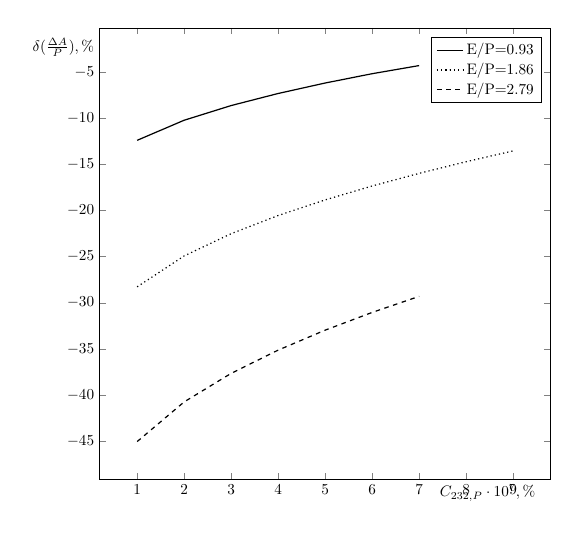
\begin{tikzpicture}[,
scale=0.55]
\begin{axis}[
  xlabel style = {{at={(axis description cs:.86,0)}}},
  ylabel = {$\delta(\frac{\Delta A}{P}), \%$},
  ylabel style = {{at={(axis description cs:-0.08,.925)},rotate=270,anchor=south}},
  xlabel = {$C_{232,P}\cdot10^{7}, \%$},
  width=12cm, height=12cm
]

\addplot+[mark=none,
  solid, black, thick
] coordinates {
  (1.0, -12.395218440946906)
  (2.0, -10.219020529323354)
  (3.0000000000000004, -8.626929870001328)
  (4.0, -7.3185844692402915)
  (5.0, -6.185264012646069)
  (6.0, -5.173768588868835)
  (7.000000000000001, -4.29293979177781)
};
\addlegendentry{{}{E/P=0.93}}

\addplot+[mark=none,
  dotted, black, thick
] coordinates {
  (1.0, -28.282242175940937)
  (2.0, -24.929077234925025)
  (3.0000000000000004, -22.516662376271356)
  (4.0, -20.550634890717415)
  (5.0, -18.85615249546271)
  (6.0, -17.34800036201673)
  (7.000000000000001, -15.978805541243855)
  (8.0, -14.71681616393461)
  (9.000000000000002, -13.541592549068923)
};
\addlegendentry{{}{E/P=1.86}}

\addplot+[mark=none,
  dashed, black, thick
] coordinates {
  (1.0, -45.057945429681226)
  (2.0, -40.758242565718376)
  (3.0000000000000004, -37.66157309459905)
  (4.0, -35.14302713983917)
  (5.0, -32.97793340752656)
  (6.0, -31.056144200883885)
  (7.000000000000001, -29.31422868906391)
};
\addlegendentry{{}{E/P=2.79}}

\end{axis}
\end{tikzpicture}


      \caption{{Зависимость экономии работы разделения от ПДК $^{232}$U в НОУ-продукте с обогащением на уровне 4,4\% для разных пропорций возврата урана.{\label{sw44}}}}
    \end{minipage}%
    \begin{minipage}{.5\textwidth}
      \centering
      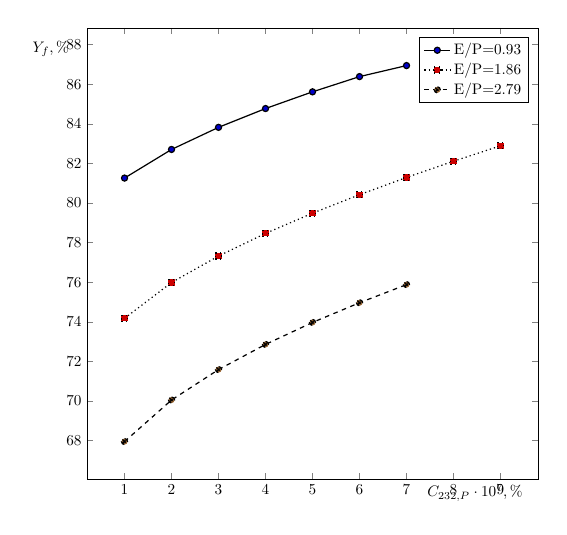
\begin{tikzpicture}[,
scale=0.55]
\begin{axis}[
  xlabel style = {{at={(axis description cs:.86,0)}}},
  ylabel = {$Y_{f}, \%$},
  ylabel style = {{at={(axis description cs:-0.08,.925)},rotate=270,anchor=south}},
  xlabel = {$C_{232,P}\cdot10^{7}, \%$},
  width=12cm, height=12cm
]

\addplot+[
  solid, black, thick
] coordinates {
  (1.0, 81.2599146274243)
  (2.0, 82.70510635581616)
  (3.0000000000000004, 83.82183689954859)
  (4.0, 84.77127401369083)
  (5.0, 85.61487919146296)
  (6.0, 86.38356067088392)
  (7.000000000000001, 86.94074198596759)
};
\addlegendentry{{}{E/P=0.93}}

\addplot+[
  dotted, black, thick
] coordinates {
  (1.0, 74.17655829999579)
  (2.0, 75.98498213201852)
  (3.0000000000000004, 77.32265969408223)
  (4.0, 78.46540402752339)
  (5.0, 79.48580928842689)
  (6.0, 80.42063662698051)
  (7.000000000000001, 81.29053109508794)
  (8.0, 82.1100269832236)
  (9.000000000000002, 82.88835691546974)
};
\addlegendentry{{}{E/P=1.86}}

\addplot+[
  dashed, black, thick
] coordinates {
  (1.0, 67.95360281561639)
  (2.0, 70.05234164130057)
  (3.0000000000000004, 71.58870177419513)
  (4.0, 72.85958391192455)
  (5.0, 73.97031718490105)
  (6.0, 74.96387446964957)
  (7.000000000000001, 75.87957963032518)
};
\addlegendentry{{}{E/P=2.79}}

\end{axis}
\end{tikzpicture}


      \caption{{Зависимость степени извлечения $^{235}$U из регенерата от ПДК $^{232}$U в НОУ-продукте с обогащением на уровне 4,4\% для разных пропорций возврата урана.{\label{exR44}}}}
    \end{minipage}
\end{figure}


\begin{figure}
    \centering
    \begin{minipage}{.5\textwidth}
      \centering
      \input{images/tex/exR_0.044}
\caption{{Зависимость степени извлечения $^{235}$U из регенерата от ПДК $^{232}$U в НОУ-продукте с обогащением на уровне 4,4\% для разных пропорций возврата урана.{\label{exR44}}}}
    \end{minipage}%
    \begin{minipage}{.5\textwidth}
      \centering
      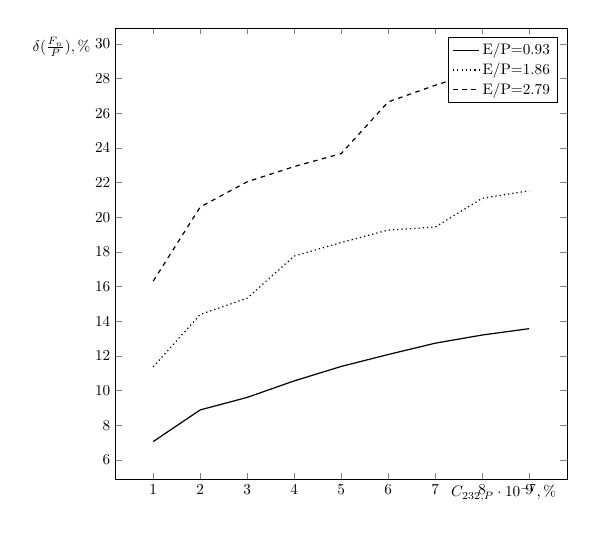
\begin{tikzpicture}[,
scale=0.55]
\begin{axis}[
  xlabel style = {{at={(axis description cs:.86,0)}}},
  ylabel = {$\delta(\frac{F_n}{P}), \%$},
  ylabel style = {{at={(axis description cs:-0.12,.925)},rotate=270,anchor=south}},
  xlabel = {$C_{232,P}\cdot10^{-7}, \%$},
  width=12cm, height=12cm
]

\addplot+[mark=none,
  solid, black, thick
] coordinates {
  (1.0, 7.057760090703368)
  (2.0, 8.883437157947327)
  (3.0000000000000004, 9.605444995054558)
  (4.0, 10.55710068193495)
  (5.0, 11.39016688359421)
  (6.0, 12.079179244566795)
  (7.000000000000001, 12.731349141503689)
  (8.0, 13.2030657848923)
  (9.000000000000002, 13.570378177156261)
};
\addlegendentry{{}{E/P=0.93}}

\addplot+[mark=none,
  dotted, black, thick
] coordinates {
  (1.0, 11.365686755446403)
  (2.0, 14.388303949542236)
  (3.0000000000000004, 15.32915753801609)
  (4.0, 17.755819239592196)
  (5.0, 18.538942955684167)
  (6.0, 19.25590180171489)
  (7.000000000000001, 19.428633887556103)
  (8.0, 21.089075670500623)
  (9.000000000000002, 21.52560986675717)
};
\addlegendentry{{}{E/P=1.86}}

\addplot+[mark=none,
  dashed, black, thick
] coordinates {
  (1.0, 16.31337535716355)
  (2.0, 20.58636758324206)
  (3.0000000000000004, 22.044054253914446)
  (4.0, 22.920132708437947)
  (5.0, 23.667999814578412)
  (6.0, 26.65031148325815)
  (7.000000000000001, 27.607494173667078)
  (8.0, 28.461707300289373)
  (9.000000000000002, 28.74364899102281)
};
\addlegendentry{{}{E/P=2.79}}

\end{axis}
\end{tikzpicture}

\caption{{Зависимость расхода природного урана от ПДК $^{232}$U в НОУ-продукте с обогащением на уровне 4,4\% для разных пропорций возврата урана.{\label{F0R44}}}}
    \end{minipage}
\end{figure}


\begin{figure}
    \centering
    \begin{minipage}{.5\textwidth}
      \centering
      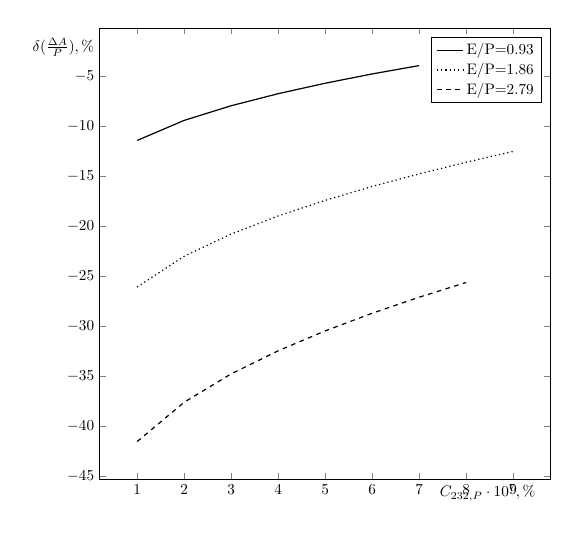
\begin{tikzpicture}[,
scale=0.55]
\begin{axis}[
  xlabel style = {{at={(axis description cs:.86,0)}}},
  ylabel = {$\delta(\frac{\Delta A}{P}), \%$},
  ylabel style = {{at={(axis description cs:-0.08,.925)},rotate=270,anchor=south}},
  xlabel = {$C_{232,P}\cdot10^{7}, \%$},
  width=12cm, height=12cm
]

\addplot+[mark=none,
  solid, black, thick
] coordinates {
  (1.0, -11.442050325962452)
  (2.0, -9.438723200431037)
  (3.0000000000000004, -7.9728246964313)
  (4.0, -6.768022196914314)
  (5.0, -5.7242794711367315)
  (6.0, -4.7922989130984135)
  (7.000000000000001, -3.956523255555432)
};
\addlegendentry{{}{E/P=0.93}}

\addplot+[mark=none,
  dotted, black, thick
] coordinates {
  (1.0, -26.09957395082424)
  (2.0, -23.022672963318332)
  (3.0000000000000004, -20.802863046158134)
  (4.0, -18.993519736891432)
  (5.0, -17.43387788617293)
  (6.0, -16.045572170953353)
  (7.000000000000001, -14.785062105867015)
  (8.0, -13.623128278493162)
  (9.000000000000002, -12.541001761914492)
};
\addlegendentry{{}{E/P=1.86}}

\addplot+[mark=none,
  dashed, black, thick
] coordinates {
  (1.0, -41.554133458995025)
  (2.0, -37.62214258113987)
  (3.0000000000000004, -34.78539667116384)
  (4.0, -32.475395453374304)
  (5.0, -30.487594682338603)
  (6.0, -28.721514147914533)
  (7.000000000000001, -27.11944341607787)
  (8.0, -25.644440494125277)
};
\addlegendentry{{}{E/P=2.79}}

\end{axis}
\end{tikzpicture}


\caption{{Зависимость экономии работы разделения от ПДК $^{232}$U в НОУ-продукте с обогащением на уровне 4,7\% для разных пропорций возврата урана.{\label{sw47}}}}
    \end{minipage}%
    \begin{minipage}{.5\textwidth}
      \centering
      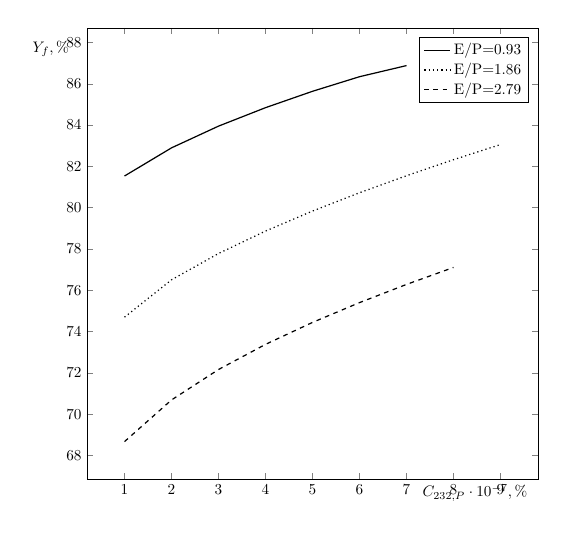
\begin{tikzpicture}[,
scale=0.55]
\begin{axis}[
  xlabel style = {{at={(axis description cs:.86,0)}}},
  ylabel = {$Y_{f}, \%$},
  ylabel style = {{at={(axis description cs:-0.08,.925)},rotate=270,anchor=south}},
  xlabel = {$C_{232,P}\cdot10^{-7}, \%$},
  width=12cm, height=12cm
]

\addplot+[mark=none,
  solid, black, thick
] coordinates {
  (1.0, 81.53156037359754)
  (2.0, 82.89545086273719)
  (3.0000000000000004, 83.9478345607235)
  (4.0, 84.84152401044177)
  (5.0, 85.63479347902604)
  (6.0, 86.3412156692256)
  (7.000000000000001, 86.88027992336104)
};
\addlegendentry{{}{E/P=0.93}}

\addplot+[mark=none,
  dotted, black, thick
] coordinates {
  (1.0, 74.69415676339759)
  (2.0, 76.50476826786495)
  (3.0000000000000004, 77.77849512744808)
  (4.0, 78.86515635925242)
  (5.0, 79.83436020530084)
  (6.0, 80.72135365193532)
  (7.000000000000001, 81.54594313296484)
  (8.0, 82.32205886834831)
  (9.000000000000002, 83.05589060957709)
};
\addlegendentry{{}{E/P=1.86}}

\addplot+[mark=none,
  dashed, black, thick
] coordinates {
  (1.0, 68.6697629941284)
  (2.0, 70.68575248489067)
  (3.0000000000000004, 72.15973261088106)
  (4.0, 73.37774759491083)
  (5.0, 74.44135268684659)
  (6.0, 75.39965734146578)
  (7.000000000000001, 76.28121651908731)
  (8.0, 77.10358771087932)
};
\addlegendentry{{}{E/P=2.79}}

\end{axis}
\end{tikzpicture}


\caption{{Зависимость степени извлечения $^{235}$U от ПДК $^{232}$U в НОУ-продукте с обогащением на уровне 4,7\% для разных пропорций возврата урана.{\label{ex47}}}}
\end{minipage}
\end{figure}

\begin{figure}
    \centering
    \begin{minipage}{.5\textwidth}
      \centering
      \input{images/tex/exR_0.047}
\caption{{Зависимость степени извлечения $^{235}$U из регенерата от ПДК $^{232}$U в НОУ-продукте с обогащением на уровне 4,7\% для разных пропорций возврата урана.{\label{exR47}}}}
    \end{minipage}%
    \begin{minipage}{.5\textwidth}
      \centering
      \begin{tikzpicture}[,
scale=0.55]
\begin{axis}[
  xlabel style = {{at={(axis description cs:.86,0)}}},
  ylabel = {$\frac{F_{NU}}{P}, \text{кг}$},
  ylabel style = {{at={(axis description cs:-0.12,.925)},rotate=270,anchor=south}},
  xlabel = {$C_{232,P}\cdot10^{7}, \%$},
  width=12cm, height=12cm
]

\addplot+[
  solid, black, thick
] coordinates {
  (1.0, 706.6354192785525)
  (2.0, 695.5705180447756)
  (3.0000000000000004, 687.235363636582)
  (4.0, 680.2789392306238)
  (5.0, 674.1924129651806)
  (6.0, 668.7266457264177)
  (7.000000000000001, 663.5511601107812)
};
\addlegendentry{{}{E/P=0.93}}

\addplot+[
  dotted, black, thick
] coordinates {
  (1.0, 677.959887355208)
  (2.0, 661.022268767328)
  (3.0000000000000004, 648.9416341028616)
  (4.0, 638.8924683215785)
  (5.0, 630.1132051976982)
  (6.0, 622.2220219123312)
  (7.000000000000001, 615.0034218929161)
  (8.0, 608.3093364348874)
  (9.000000000000002, 602.0503886358283)
};
\addlegendentry{{}{E/P=1.86}}

\addplot+[
  dashed, black, thick
] coordinates {
  (1.0, 654.2885822321769)
  (2.0, 632.4090216922981)
  (3.0000000000000004, 616.5981030031621)
  (4.0, 603.7017776368674)
  (5.0, 592.5838268649425)
  (6.0, 582.6875967531196)
  (7.000000000000001, 573.6906309431884)
  (8.0, 565.3894655334504)
};
\addlegendentry{{}{E/P=2.79}}

\end{axis}
\end{tikzpicture}


\caption{{Зависимость расхода природного урана от ПДК $^{232}$U в НОУ-продукте с обогащением на уровне 4,7\% для разных пропорций возврата урана.{\label{F0R47}}}}
\end{minipage}
\end{figure}


\begin{figure}
    \centering
    \begin{minipage}{.5\textwidth}
      \centering
      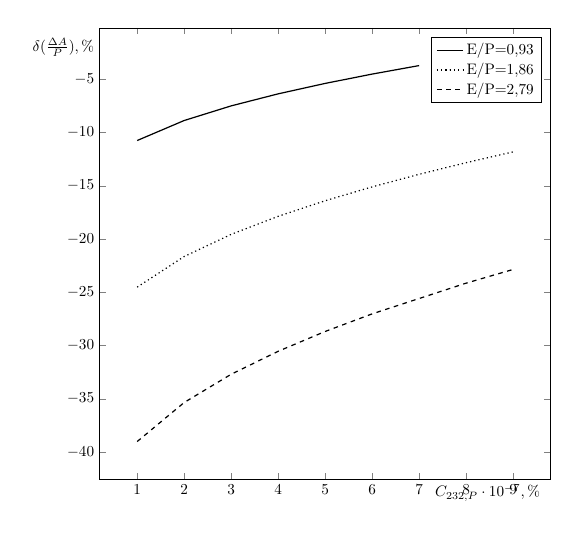
\begin{tikzpicture}[,
scale=0.55]
\begin{axis}[
  xlabel style = {{at={(axis description cs:.86,0)}}},
  ylabel = {$\delta(\frac{\Delta A}{P}), \%$},
  ylabel style = {{at={(axis description cs:-0.08,.925)},rotate=270,anchor=south}},
  xlabel = {$C_{232,P}\cdot10^{-7}, \%$},
  width=12cm, height=12cm
]

\addplot+[mark=none,
  solid, black, thick
] coordinates {
  (1.0, -10.75592874548788)
  (2.0, -8.877549872366233)
  (3.0000000000000004, -7.50289958013979)
  (4.0, -6.3729908570898814)
  (5.0, -5.39405720345885)
  (6.0, -4.517136753769094)
  (7.000000000000001, -3.717964070419745)
};
\addlegendentry{{}{E/P=0,93}}

\addplot+[mark=none,
  dotted, black, thick
] coordinates {
  (1.0, -24.523693715258393)
  (2.0, -21.64946440952475)
  (3.0000000000000004, -19.56910789260241)
  (4.0, -17.87302824962024)
  (5.0, -16.41089275400384)
  (6.0, -15.109277255129713)
  (7.000000000000001, -13.927405951747463)
  (8.0, -12.837656298351746)
  (9.000000000000002, -11.820833744285492)
};
\addlegendentry{{}{E/P=1,86}}

\addplot+[mark=none,
  dashed, black, thick
] coordinates {
  (1.0, -39.02572435708815)
  (2.0, -35.35744140949972)
  (3.0000000000000004, -32.707361682832236)
  (4.0, -30.547279725027575)
  (5.0, -28.687040100935018)
  (6.0, -27.03315569727767)
  (8.0, -24.149000859531828)
  (9.000000000000002, -22.860928202940787)
};
\addlegendentry{{}{E/P=2,79}}

\end{axis}
\end{tikzpicture}


\caption{{Зависимость экономии работы разделения от ПДК $^{232}$U в НОУ-продукте с обогащением на уровне 4,95\% для разных пропорций возврата урана.{\label{sw495}}}}
    \end{minipage}%
    \begin{minipage}{.5\textwidth}
      \centering
      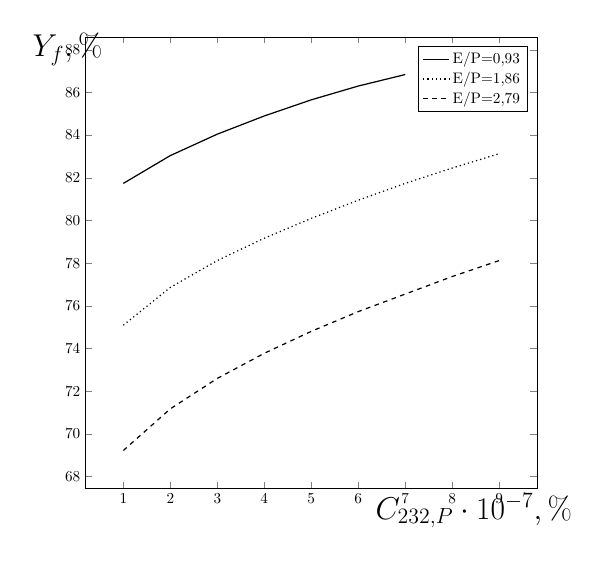
\begin{tikzpicture}[,
scale=0.55]
\begin{axis}[
  xlabel style = {{at={(axis description cs:.86,0)},font=\fontsize{22}{22}\selectfont}},
  ylabel = {$Y_{f}, \%$},
  ylabel style = {{at={(axis description cs:-0.04,.925)},rotate=270,anchor=south,font=\fontsize{22}{22}\selectfont}},
  xlabel = {$C_{232,P}\cdot10^{-7}, \%$},
  width=12cm, height=12cm
]

\addplot+[mark=none,
  solid, black, thick
] coordinates {
  (1.0, 81.73497884138504)
  (2.0, 83.03778477520555)
  (3.0000000000000004, 84.04194826713017)
  (4.0, 84.89394805905036)
  (5.0, 85.64964216184214)
  (6.0, 86.29627615264738)
  (7.000000000000001, 86.83475753524942)
};
\addlegendentry{{}{E/P=0,93}}

\addplot+[mark=none,
  dotted, black, thick
] coordinates {
  (1.0, 75.09103641667504)
  (2.0, 76.86408581728926)
  (3.0000000000000004, 78.1230950450531)
  (4.0, 79.16703478387757)
  (5.0, 80.0973214088445)
  (6.0, 80.94802830843058)
  (7.000000000000001, 81.73831087619449)
  (8.0, 82.45610633767066)
  (9.000000000000002, 83.12799096181396)
};
\addlegendentry{{}{E/P=1,86}}

\addplot+[mark=none,
  dashed, black, thick
] coordinates {
  (1.0, 69.22294832705394)
  (2.0, 71.17489372337026)
  (3.0000000000000004, 72.60072511995082)
  (4.0, 73.77803561909946)
  (5.0, 74.80542388393039)
  (6.0, 75.73053709257948)
  (8.0, 77.37433736075826)
  (9.000000000000002, 78.12192420776128)
};
\addlegendentry{{}{E/P=2,79}}

\end{axis}
\end{tikzpicture}


\caption{{Зависимость степени извлечения $^{235}$U от ПДК $^{232}$U в НОУ-продукте с обогащением на уровне 4,95\% для разных пропорций возврата урана.{\label{ex495}}}}
\end{minipage}
\end{figure}

\begin{figure}
    \centering
    \begin{minipage}{.5\textwidth}
      \centering
      \input{images/tex/exR_0.0495}
\caption{{Зависимость степени извлечения $^{235}$U из регенерата от ПДК $^{232}$U в НОУ-продукте с обогащением на уровне 4,95\% для разных пропорций возврата урана.{\label{exR495}}}}
    \end{minipage}%
    \begin{minipage}{.5\textwidth}
      \centering
      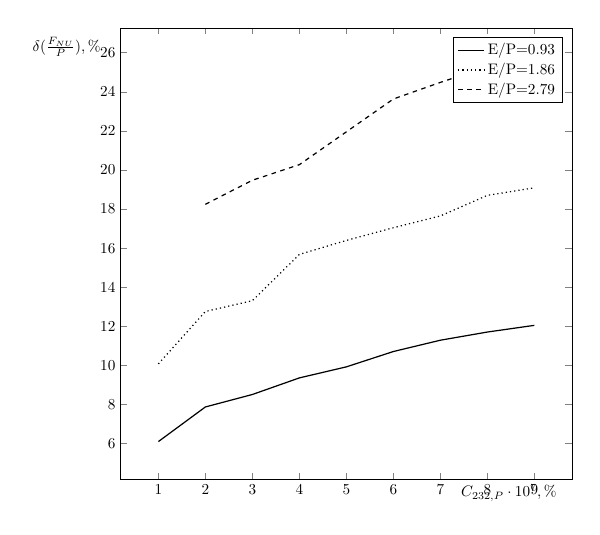
\begin{tikzpicture}[,
scale=0.55]
\begin{axis}[
  xlabel style = {{at={(axis description cs:.86,0)}}},
  ylabel = {$\delta(\frac{F_{NU}}{P}), \%$},
  ylabel style = {{at={(axis description cs:-0.12,.925)},rotate=270,anchor=south}},
  xlabel = {$C_{232,P}\cdot10^{7}, \%$},
  width=12cm, height=12cm
]

\addplot+[mark=none,
  solid, black, thick
] coordinates {
  (1.0, 6.102609628967004)
  (2.0, 7.873257521230414)
  (3.0000000000000004, 8.510982187035465)
  (4.0, 9.359903696758797)
  (5.0, 9.924557345258734)
  (6.0, 10.709375471912841)
  (7.000000000000001, 11.287587970677283)
  (8.0, 11.705810902202751)
  (9.000000000000002, 12.048111265678951)
};
\addlegendentry{{}{E/P=0.93}}

\addplot+[mark=none,
  dotted, black, thick
] coordinates {
  (1.0, 10.07679447624098)
  (2.0, 12.756640615222503)
  (3.0000000000000004, 13.309773249935485)
  (4.0, 15.676539853992955)
  (5.0, 16.39235800951654)
  (6.0, 17.041722793102686)
  (7.000000000000001, 17.64593776461374)
  (8.0, 18.69753065296348)
  (9.000000000000002, 19.08456096001587)
};
\addlegendentry{{}{E/P=1.86}}

\addplot+[mark=none,
  dashed, black, thick
] coordinates {
  (2.0, 18.241079567317232)
  (3.0000000000000004, 19.47072745723193)
  (4.0, 20.268597025731783)
  (6.0, 23.628111214220738)
  (7.000000000000001, 24.476747414958155)
  (8.0, 25.273745846887998)
  (9.000000000000002, 25.337305198229632)
};
\addlegendentry{{}{E/P=2.79}}

\end{axis}
\end{tikzpicture}

\caption{{Зависимость расхода природного урана от ПДК $^{232}$U в НОУ-продукте с обогащением на уровне 4,95\% для разных пропорций возврата урана.{\label{F0R495}}}}
\end{minipage}
\end{figure}

    
По осям ординат на графиках \ref{sw44}-\ref{F0R495} представлены основные характеристические показатели: $\delta(\frac{\Delta U}{P})$ -- экономия работы разделения по сравнению с ординарным каскадом, питаемым природным ураном, получающим продукт с эквивалентной эффективной концентрацией $^{235}$U; степени извлечения $^{235}$U в схеме $R_f$ и из регенерата $R_{RepU}$, а также удельный расход природного урана $\delta(\frac{F_{NU}}{P})$.

Анализ графиков \ref{sw44}-\ref{F0R495} позволяет сделать заключение о применимости схемы двойного каскада с НОУ-разбавителем для задачи полного возврата массы регенерата в ядерный топливный цикл в условиях многократного рецикла даже в условиях жестких ограничений на содержание $^{232}U$, чем современные требования, а также при более ограничивающем условии задействовании двух единиц облученного топлива для производства одной единицы НОУ-продукта, так как производимый конечный продукт удовлетворяет заданным ограничениям на четные изотопы.

При этом, как показывает анализ результатов, представленных на графиках \ref{sw44}-\ref{F0R495}, уменьшение допустимой концентрации $^{232}$U в продукте при фиксированном отношении исходного регенерата к товарному НОУ обусловливает ухудшение всех исследуемых ключевых показателей. Однако, из этих показателей, существенно лишь падение степени извлечения $^{235}$U из регенерата при более строго ограничении на $^{232}$U, тогда как значительного увеличения расхода природного урана, увеличения числа центрифуг в каскадной схем (работы разделения), или значимого ухудшения извлечения $^{235}$U в схеме не наблюдается.


\section{Общие выводы по результатам анализа схемы двойного каскада с НОУ-разбавителем}

В качестве обобщающих выводов по результатам анализа схемы двойного каскада с НОУ-разбавителем (рис. \ref{p2left}), обозначим следующее:
\begin{enumerate}
    \item схема применима для обогащения регенерированного урана в условиях многократного рецикла урана в топливе легководных реакторов, поскольку позволяет получать продукт, отвечающий всем требованиям на концентрации четных изотопов для регенерата различного исходного состава, включая рециклы, к которым накопилось повышенное содержание четных изотопов (на примере пятого рецикла);
    \item схема позволяет отделить участки обогащения регенерированного урана (где разделительное оборудование будет подвержено загрязнению минорными изотопами) от каскадов, обогащающих не содержащий $^{232,236}$U природный уран или ОГФУ. При этом доля разделительных мощностей, отводимых под работу с регенерированным ураном при наработке НОУ для загрузки реактора составляет не более 10\%;
    \item содержание изотопов $^{232,234}$U в отвале каскада 1 на порядки ниже предельно допустимых нормативных значений, что делает возможным долговременное хранение подобного отвала в виде гексафторида урана или его перевод в другое, более удобное химическое соединение, например, на установках дефторирования, таких как W-ЭХЗ \cite{oecdManagementDepletedUranium2001};
    \item в схеме на каждом рецикле происходит накопление побочно производимого материала -- высокоактивного отхода (отбор второго каскада), в котором к тому же происходит потеря делящегося $^{235}$U. Стратегии дальнейшего обращения с данным отходом требуют отдельного анализа. Одним из вариантов решения этой проблемы является его перемешивание с отвалом каскада 1.
    \item работа схемы связана с потерями работы разделения при двух этапах производственного процесса:
    \begin{enumerate}
        \item обеднение отбора первого каскада $P_1$ во втором каскаде;
        \item смешивание потоков $W_2$ с НОУ-разбавителем $P_0$, в которых различается содержание изотопа $^{235}$U;
    \end{enumerate}
\end{enumerate}

Отсюда, достоинствами рассматриваемой каскадной схемы являются:

\begin{enumerate}
    \item возможность полностью решить задачу возврата всей массы регенерированного урана в условиях многократного рецикла;
    \item частичное очищение регенерированного урана от четных изотопов $^{232,233,234}$U;
    \item обогащение даже загрязненного четными изотопами регенерированного урана, что делает схему применимой в условиях многократного рецикла всей массы регенерированного урана;
    \item загрязнение меньшей доли разделительных мощностей четными изотопами, чем у разбавляющих каскадов, рассмотренных в главе 1, так как занятые под получение разбавителя остаются незагрязненными четными изотопами. Вдобавок, такой подход позволяет легко переориентировать ту часть разделительных мощностей, которая не соприкасалась с регенератом (поскольку разбавление происходит вне каскадов), на решение других задач;
    \item концентрации изотопов $^{232,233,234}$U в потоке $W_1$ снижены по отношению к концентрациям в потоке $E$ более чем на порядок, что делает хранение такой фракции более безопасным, чем хранение исходного регенерированного урана. Если же смешать отвальные потоки каскадной схемы ($W_1$  и $W_3$), получившийся обедненный уран будет иметь концентрации четных изотопов на несколько порядков ниже допустимых значений, что позволяет говорить о возможности его безопасного хранения и, при необходимости, последующего прямого обогащения до уровня НОУ;
\end{enumerate}

Основными недостатками рассматриваемой каскадной схемы, также как и рассмотренных ранее двойных каскадов, являются: 
\begin{enumerate}
    \item наличие «побочного» продукта в виде относительно небольшого (до 1–3\% от общей массы входящего потока регенерата) количество отхода -- загрязненной фракции, в которой преимущественно сконцентрированы изотопы $^{232,233,234}$U, а также обогащен $^{235}$U;
    \item потери работы разделения при смешивании потоков с различным содержанием  $^{235}$U.
\end{enumerate}





\section{Рассмотрение различных возможностей утилизации легкой фракции второго каскада в схеме}

\subsection{Анализ возможности утилизации легкой фракции путем ее перемешивания с регенератом, поступающим на обогащение}

\subsubsection{Описание схемы двойного каскада с НОУ-разбавителем с возвратом потока $P_2$ в цикл}

В качестве модификации каскадной схемы, представленной на рис. \ref{P2utilizationRing} предложен способ, позволяющий вернуть поток $P_2$ в топливный цикл для производства НОУ-продукта (рис. \ref{p2left}) \cite{nevinicaToplivnyyCiklLegkovodnogo2019, nevinicaSposobIzotopnogoVosstanovleniya2019}. Принцип ее работы состоит в следующем.

\begin{figure}[ht]
    \centerfloat{\includegraphics[scale=0.6]{cascades/P2utilizationRing}}
    \caption{Схема передачи загрязненной изотопом $^{232}$U фракции гексафторида урана в двойном каскаде от первой партии дообогащенного регенерированного урана к последующей. Обозначения: $E$ -- поток регенерированного урана; $P_1$ -- поток отбора первого каскада, выступающий питанием второго каскада; $P_2$ -- поток отбора второго каскада; $W_1$ -- поток отвала первого каскада; $W_2$ -- поток тяжелой фракции (условный «отвал») второго каскада; $P_0$ -- поток НОУ-разбавителя; $P$ -- финальный продукт (товарный низкообогащенный уран (НОУ), который подается на питание последующего двойного каскада, перемешиваясь с регенератом очередного рецикла}\label{P2utilizationRing}
\end{figure}

Учитывая, что каскадная схема двойного каскада с НОУ-разбавителем (рис. \ref{p2left}) предназначена для обогащения регенерата с высоким накопившимся в ходе серии пройденных рециклов содержанием изотопа $^{232}$U, можно использовать такую каскадную схему для вовлечения ранее полученного в потоке отбора второго каскада фракции $P_2$ загрязненной изотопом $^{232}$U. Выведенный ранее из системы гексафторида урана может быть перемешан с регенератом, полученным из следующей партии отработавшего топлива, то есть с составом более загрязненным изотопами $^{232,233,234,236}$U, чем исходно использовавшийся состав, побочным продуктом которого оказался этот $P_2$. Полученная таким образом в результате смешения $P_2$ предыдущего рецикла и регенерата очередного рецикла смесь будет отправлена на последующее обогащение (рис. \ref{P2utilizationRing}).

При использовании подобной схемы удастся полностью замкнуть топливный цикл по урану, а единственным отходом производства останется ОГФУ, образующийся в отвале первого каскада, который можно считать штатным отходом обогатительного производства с отработанными технологиями хранения и переработки. При этом после завершения производственного цикла останется невостребованным только та масса обогащенного по изотопу $^{232}$U гексафторида урана (загрязненной фракции легкого конца второго каскада (рис. \ref{P2utilizationRing})), которая будет образована после обогащения последней партии регенерата. Таким образом, предложенный подход к дообогащению регенерата урана позволяет организовать полный возврат массы регенерированного урана в топливный цикл в течение всего жизненного цикла задействованного урана.

При схожем наборе достоинств и недостатков схемы двойного каскада с НОУ-разбавителем с возвратом потока $P_2$ в цикл (рис. \ref{P2utilizationRing}), достоинством схемы с возвратом $P_2$ является более глубокая выработка потенциала делящегося $^{235}$U, накапливаемого совместно с изотопами $^{232,233,234}$U в загрязненной фракции второго каскада. Это позволяет добиваться меньших потерь $^{235}$U на всем жизненном цикле используемого урана.



Как видно из данных табл. \ref{vest2019_2} предложенная схема рециклирования действительно позволяет полностью израсходовать и исходный регенерированный уран и образующийся в результате использования двойного каскада высокообогащенный отход.

Итак, опираясь на результаты расчетов, можно сделать общие выводы касаемо двойного каскада с НОУ-разбавителем с возвратом потока $P_2$ в цикл:

\begin{enumerate}
    \item схема принципиально применима для обогащения регенерированного урана в условиях многократного рецикла урана в топливе легководных реакторов, поскольку позволяет получать продукт, отвечающий всем требованиям по концентрациям четных изотопов для регенерата различного исходного состава;
    \item достоинством схемы является полное отсутствие потерь $^{235}$U (не считая потока отвала первого каскада) в процессе рециклирования, а также полное отсутствие нештатного отхода вплоть до последней перегрузки последнего рецикла; Однако, ввиду искусственного повышения содержания четных изотопов $^{232,234}$U в получаемом продукте с каждой последующей перегрузкой возрастает масса отхода  $P_2$ и, соответственно, масса концентрирующегося в нем изотопа $^{235}$U, что уменьшает эффект от возврата изотопа $^{235}$U в цикл из-за его потерь вследствие увеличения потока загрязненной фракции, которое происходит вследствие роста концентраций четных изотопов в исходной смеси.
    \item возврат фракции отхода (потока $P_2$) в схему является причиной монотонного роста концентраций четных изотопов, что приводит к необходимости увеличения уровня обогащения получаемого НОУ и, тем самым, к росту затрат работы разделения, а также повышению концентрации изотопа $^{235}$U в НОУ-разбавителе ввиду необходимости компенсации влияния $^{236}$U;
    \item в схеме присутствуют потери работы разделения из-за необходимости обеднять отбор второго ординарного каскада $P_2$ в последующей составной каскадной схеме;
\end{enumerate}


В качестве общего вывода по результатам анализа схемы двойного каскада с НОУ-разбавителем с возвратом $P_2$ в топливный цикл (рис. \ref{p2left}) представим следующее:
\begin{enumerate}
    \item схема применима для обогащения регенерированного урана в условиях многократного рецикла урана в топливе легководных реакторов, поскольку позволяет получать продукт, отвечающий всем требованиям на концентрации четных изотопов на основе состава регенерата с повышенным исходным содержанием изотопов $^{232,234}$U, который не позволяет решить проблему с помощью ординарного каскада;
    \item схема позволяет использовать поток «легкой» фракции второго каскада ($P_2$), поскольку указанный поток возвращается в топливный цикл, что снимает проблемы его долговременного хранения и связанные с ним затраты;
    \item схема c возвратом $P_2$ как и предшествующая схема без возврата $P_2$, подходит для решения задачи обогащения урана при одновременном выполнении всех сопутствующих условий, в том числе, при обогащении регенерированного урана, прошедшего несколько последовательных рециклов;
    \item схема c возвратом $P_2$ как и предшествующая схема двойного каскада с НОУ-разбавителем, позволяет задействовать для воспроизводства ядерного топлива накопленный в значительных количествах обедненный уран. Производимый ею отвал регенерированного урана ($W_1$) имеет содержание четных изотопов на уровне ниже допустимых ограничений. Это позволяет говорить о том, что такие отвалы могут безопасно длительно хранится в виде гексафторида урана или быть переработанными на установке дефторирования;
    \item в схеме на трех стадиях процесса обогащения происходят потери работы разделения:
    \begin{enumerate}
        \item обеднение отбора первого каскада $P_1$ во втором каскаде;
        \item смешивание потоков $W_2$ с НОУ-разбавителем $P_0$, в которых различается содержание изотопа $^{235}$U;
        \item смешивания потоков $P_2$ и $E$ на входе в каскады, принимающие регенерат последующих рециклов (начиная с третьего).
    \end{enumerate}
    \item в схеме, как и в предшествующей немодифицированной схеме двойного каскада с НОУ-разбавителем, физически разделены участки каскада с разделительным оборудованием, пропускающие через себя регенерированный урана (первые два каскады, принимающие на вход поток $E$ на рисунке \ref{P2utilizationRing}) и участок обогащения сырья для наработки НОУ-разбавителя -- природного или обедненного урана -- материалов, которые не загрязнены четными изотопами $^{232,236}$U. В дальнейшем это позволит задействовать оборудование каскада, использовавшегося для наработки разбавителя, в операциях обогащения природного урана или другого сырьевого материала, не загрязненного четными изотопами, а значит в менее жестконормированных условиях эксплуатации;
    \item практическая реализация представляется нецелесообразной, поскольку данная схема не дает ощутимых преимуществ с точки зрения интегральной экономии $^{235}$U в топливном цикле по отношению к схеме двойного каскада с НОУ-разбавителем (рис. \ref{p2left}), причем реализации схемы с возвратом $P_2$ возможна только в условиях непрерывной работы реактора и постоянного поступления новых партий регенерата на дообогащение.
\end{enumerate}



Заметим, что процесс возврата данного материала в воспроизводство низкообогащенного урана может быть начат также и после дообогащения регенерата уже для одной ТВС и даже для ее части (непрерывный возврат). В этом случае также удастся полностью замкнуть топливный цикл по урану, а единственным отходом производства станет обедненный гексафторид, образующийся в отвале первого каскада, который можно считать штатным отходом обогатительного производства, для которого на сегодняшний день отработаны технологии хранения и переработки.

При этом после вывода завода из эксплуатации (или остановки на планово-предупредительный ремонт) останется невостребованным только та масса обогащенного по изотопу $^{232}$U гексафторида урана, которая будет образована после обогащения последней партии регенерата на этом заводе. Таким образом, рассматриваемый подход к дообогащению регенерата урана позволяет организовать полный возврат регенерированного урана в топливный цикл в течение практически всего жизненного цикла топлива легководных реакторов, работающих в замкнутом топливном цикле.

Несмотря на очевидные достоинства рассматриваемого способа, возникает вопрос о его эффективности с точки зрения интегральных характеристик разделительного каскада, важных для экономики топливного цикла в целом. Речь идет об экономии природного урана в цикле и затратах работы разделения на единицу массы готового НОУ.
В связи с этим целью настоящей работы явилась оценка интегральных показателей для рассматриваемой схемы в условиях ее использования для обогащения регенерированного урана и наработки НОУ для обеспечения поставок для формирования топлива нескольких последовательных загрузок реактора.

Исходный регенерат второго рецикла использован для производства тепловыделяющих сборок (ТВС) c обогащением: 4,95\%. Из указанного состава изготавливают сначала топливо для первой перегрузки. Далее, загрязненную фракцию от обогащения регенерата для первой перегрузки перемешивают с регенератом исходного состава для второго рецикла и направляют на последующее обогащение для получения топлива следующей перегрузки. Всего рассмотрено 7 перегрузок. При расчете состава низкообогащенного урана после каскада при получении топлива для каждой из перегрузок решается оптимизационную задачу (метод прямого поиска) для шести выбранных критериев эффективности при шаге по концентрации в потоке отбора первого каскада и потоках отбора и отвала второго каскада равном 1\%. Для сопоставления отбирали только те варианты, для которых выполнены описанные выше условия для концентраций четных изотопов. Диапазоны варьирования концентраций в выходящих потоках каскадной схемы были следующими. Концентрацию $^{235}$U в первом каскаде варьировали в диапазоне 7-17\%, в отвале второго каскада 6-16\%, в отборе второго каскада 10-20\%.

Ввиду сложности многокритериального анализа для каждой из перегрузок был рассмотрен случай с параллельными «ветками», на каждой из которых проводили последовательный расчет изотопных составов и параметров разделительного каскада для семи перегрузок, при условии оптимизации на каждом из шагов по одному и тому же критерию эффективности. В качестве критериев эффективности выступали величины: (1) минимум расхода природного урана на единицу продукта, (2) минимум затрат работы разделения на единицу продукта, (3) минимум концентрации изотопа $^{232}$U (в диапазоне 2-$5\cdot10^{-7}$\%), (4) минимум концентрации изотопа $^{236}$U, (5) минимум массы отхода двойного каскада, (6) максимум степени извлечения $^{235}$U из поступающего в обогащение регенерата. Под степенью извлечения $^{235}$U из исходного регенерированного урана понимали отношение массы $^{235}$U в отвале второго каскада к массе $^{235}$U в исходной смеси регенерата, поступившего для обогащения.

Далее представлены результаты проведенных вычислительных экспериментов и проведен их анализ. 
На рисунке \ref{3} представлено изменение удельного расхода природного урана при получении товарного НОУ при шести различных критериях эффективности, по которым осуществляли оптимизацию для каждой перегрузки. Как следует из анализа зависимостей, показанных на указанном рисунке при оптимизации по четырем, а именно: минимуму удельного расхода природного урана, минимуму удельных затрат работы разделения, минимуму массы отхода двойного каскада, максимуму степени извлечения $^{235}$U из поступающего в обогащение регенерата, зависимости практически совпадают. Это можно объяснить тем, что данные критерии близки по своей сути. Например, максимум степени извлечения $^{235}$U из поступающего в обогащение регенерата должен приводить к необходимости использования минимальной массы $^{235}$U из природного сырья, что и выражается в уменьшении расхода природного сырья. В целом все кривые представляют собой уменьшающиеся функции, что логично, учитывая, что с каждой перегрузкой масса исходного регенерата возрастает одновременно с повышением концентрации $^{235}$U в нем. Однако при использовании в качестве критериев эффективности минимумов концентраций $^{232}$U и $^{236}$U в товарном НОУ соответствующие кривые заметно отличаются от четырех упомянутых выше случаев. Как можно видеть из рисунка \ref{3} (кривые 4 и 5) для этих случаев характерен заметно больший расход природного урана. Данный факт можно объяснить тем, что при оптимизации по минимуму концентраций четных изотопов в товарном НОУ происходит «вытеснение» четных изотопов, а вместе с ними и значительной массы $^{235}$U в отбор второго каскада. В результате заметно падает степень извлечения $^{235}$U из исходного регенерата (рисунок \ref{4}) и масса отхода, что отчетливо заметно по зависимостям на рисунке \ref{5}, в соответствии с которыми масса отхода для этих критериев на последних перегрузках превышает массу исходного регенерата и составляет величину более 30\% от массы исходного регенерата. В то время как для других критериев эта величина даже на 7-й перегрузке не превышает 10\%. Общей закономерностью для всех случаев является снижение расхода природного сырья с каждой перегрузкой (рисунок \ref{6}).


\begin{figure}[ht]
    \begin{minipage}{.5\textwidth}
      \centering
      \includegraphics[width=.8\linewidth]{images/net/3}  
      \caption{Изменение величины удельного расхода природного урана в двойном каскаде с замыканием в зависимости от номера перегрузки для обогащения 4,95\% для различных критериев эффективности.}
      \label{3}
    \end{minipage}
    \begin{minipage}{.5\textwidth}
      \centering
      \includegraphics[width=.8\linewidth]{images/net/4}  
      \caption{Степень извлечения $^{235}$U из исходного регенерата в зависимости от номера перегрузки для обогащения 4,95\% для различных критериев эффективности.}
      \label{4}
    \end{minipage}
    \begin{minipage}{.5\textwidth}
      \centering
      \includegraphics[width=.8\linewidth]{images/net/5}  
      \caption{Величину удельного отхода (на единицу исходного регенерата) в зависимости от номера перегрузки для обогащения 4,95\% для различных критериев эффективности.}
      \label{5}
    \end{minipage}
    \begin{minipage}{.5\textwidth}
      \centering
      \includegraphics[width=.8\linewidth]{images/net/6}  
      \caption{Относительное изменение величины удельного расхода природного урана в двойном каскаде с замыканием в зависимости от номера перегрузки для обогащения 4,95\% для различных критериев эффективности.}
      \label{6}
    \end{minipage}
\end{figure}


Обозначения для рис. \ref{3}–\ref{6} приняты следующие. Кривая 1: оптимумы по расходу природного урана, кривая 2: оптимумы по затратам работы разделения, кривая 3: оптимумы по массе высокообогащенной фракции, кривая 4: минимум концентрации $^{232}$U, кривая 5: минимум концентрации $^{236}$U, кривая 6: максимум степени извлечения минимум $^{235}$U из регенерата урана.

В результате описанных выше процессов увеличивается и достигает значений, близких к 2, величина отношения (исходный регенерат)/продукт (риc. \ref{7}). Анализ зависимостей концентраций $^{235}$U и четных изотопов в регенерате, поступающем на обогащение после смешивания с высокообогащенной фракцией показывает, что все они повышается с каждой перегрузкой (рисунки \ref{8}–\ref{11}). Однако при использовании в качестве критериев эффективности минимумов концентраций  $^{232}$U и  $^{236}$U в товарном НОУ концентрации всех указанных выше изотопов в исходном регенерате возрастают заметно интенсивнее. Важно при этом отметить, что на последних перегрузках концентрация $^{235}$U в исходном регенерате превышает величину, требуемую для финального продукта (рисунок \ref{11}). Это означает, что схема начинает обеднять смесь и «чистить» ее от четных, а не обогащать. Особенно сильно это проявляется при минимизации концентраций четных изотопов в продукте, поскольку в этих случаях концентрация $^{235}$U в исходном регенерате могут приближаться к 5\% (рисунок \ref{10}). Подобные результаты говорят, в первую очередь, о нецелесообразности использования схемы в таком варианте для последовательного обогащения регенерата нескольких перегрузок с использованием в качестве критериев эффективности на каждом шаге требования минимальности концентраций $^{232}$U и  $^{236}$U в товарном НОУ. Однако требуют дополнительных исследований возможности дальнейшей модификации предложенной схемы, в том числе, для более эффективного использования исходного регенерата с повышенным содержанием $^{235}$U. Одним из таких вариантов может стать расширение диапазона увеличения концентрации  $^{235}$U в схеме, например, до 90\%. Другие варианты могут быть основаны на введении дополнительных потоков для разбавления четных изотопов и снижения концентрации  $^{235}$U до нужных значений.

\begin{figure}[ht]
    \centerfloat{\includegraphics[scale=0.7]{images/net/7}}
    \caption{Зависимость отношения потоков исходного регенерата и финального продукта (товарного НОУ) от номера перегрузки для обогащения 4,95\% для различных критериев эффективности.}\label{7}
\end{figure}

\begin{figure}[ht]
    \begin{minipage}{.5\textwidth}
      \centering
      \includegraphics[width=.8\linewidth]{images/net/8}  
      \caption{Зависимость концентрации $^{232}$U в исходном регенерате от номера перегрузки для обогащения 4,95\% для различных критериев эффективности.}
      \label{8}
    \end{minipage}
    \begin{minipage}{.5\textwidth}
      \centering
      \includegraphics[width=.8\linewidth]{images/net/9}  
      \caption{Зависимость концентрации $^{234}$U в исходном регенерате от номера перегрузки для обогащения 4,95\% для различных критериев эффективности.}
      \label{9}
    \end{minipage}
    \begin{minipage}{.5\textwidth}
      \centering
      \includegraphics[width=.8\linewidth]{images/net/10}  
      \caption{Зависимость концентрации $^{235}$U в исходном регенерате от номера перегрузки для обогащения 4,95\% для различных критериев эффективности.}
      \label{10}
    \end{minipage}
    \begin{minipage}{.5\textwidth}
        \centering
        \includegraphics[width=.8\linewidth]{images/net/11}  
        \caption{Зависимость концентрации $^{236}$U в исходном регенерате от номера перегрузки для обогащения 4,95\% для различных критериев эффективности.}
        \label{11}
      \end{minipage}
\end{figure}

Обозначения для рис. \ref{7}–\ref{11} приняты следующие. Кривая 1: оптимумы по расходу природного урана, кривая 2: оптимумы по затратам работы разделения, кривая 3: оптимумы по массе высокообогащенной фракции, кривая 4: минимум концентрации $^{232}$U, кривая 5: минимум концентрации $^{236}$U, кривая 6: максимум степени извлечения минимум $^{235}$U из регенерата урана), E – поток питающего каскадную схему регенерата, P -- товарный НОУ.


Анализ изменения величины затрат работы разделения в зависимости от номера перегрузки и выбранного критерия эффективности показывает следующее. Для всех критериев, кроме случаев минимизации концентрации $^{232}$U или $^{236}$U затраты работы разделения сохраняются на определенном уровне, незначительно отличающемся от случая обогащения природного урана до соответствующей концентрации (рисунок \ref{12}). С увеличением номера перегрузки происходит незначительное снижение потерь работы разделения для этих случаев: с $\approx$5\% до $\approx$10\% (рисунок \ref{13}). При этом в случае минимизации концентраций изотопов $^{232}$U или $^{236}$U затраты работы разделения значительно выше и  могут на десятки процентов превосходить аналогичные затраты для случая обогащения природного урана для получения эквивалентного количества требуемого НОУ.

\begin{figure}[ht]
    \begin{minipage}{.5\textwidth}
      \centering
      \includegraphics[width=.8\linewidth]{images/net/12}  
      \caption{Изменение величины удельных затрат работы разделения в двойном каскаде с замыканием в зависимости от номера перегрузки для обогащения 4,95\% для различных критериев эффективности.}
      \label{12}
    \end{minipage}
    \begin{minipage}{.5\textwidth}
      \centering
      \includegraphics[width=.8\linewidth]{images/net/13}  
      \caption{Относительное изменение величины удельных затрат работы разделения в двойном каскаде с замыканием в зависимости от номера перегрузки для обогащения 4,95\% для различных критериев эффективности.}
      \label{13}
    \end{minipage}
\end{figure}

Обозначения для рис. \ref{12}–\ref{13} приняты следующие. Кривая 1: оптимумы по расходу природного урана, кривая 2: оптимумы по затратам работы разделения, кривая 3: оптимумы по массе высокообогащенной фракции, кривая 4: минимум концентрации $^{232}$U, кривая 5: минимум концентрации $^{236}$U, кривая 6: максимум степени извлечения минимум $^{235}$U из регенерата урана.

Рассматриваемая каскадная схема может работать в широком диапазоне изменения концентраций компонентов, в первую очередь, четных изотопов и $^{235}$U в исходном регенерате. Данный факт открывает возможности для применения схемы в условиях топливных циклов с увеличенной длительностью топливного цикла, а также в условиях многократного рецикла урана.

В зависимости от выбранного критерия эффективности для оптимизации схемы при расчете изотопного состава НОУ для каждой новой перегрузки, возможно обеспечить широкую вариативность параметров рассматриваемой каскадной схемы. При этом в случае выбора в качестве критериев эффективности величин удельного расхода природного урана, удельных затрат работы разделения, массы получаемого отхода или величины степени извлечения $^{235}$U из исходного регенерата оптимальные параметры схемы меняются незначительно. В то время, как при использовании в качестве критериев эффективности условий минимума концентраций $^{232}$U и $^{236}$U в товарном НОУ ключевые характеристики каскадов значительно отличаются от других критериев.

С ростом номера перегрузки происходит последовательно уменьшение расхода природного урана и затрат работы разделения. При этом на последних перегрузках экономия природного урана достигает величины 20\% и более. Это означает, что экономия природного урана в цикле в среднем будет примерно на треть выше типичного значения в 15\%. Причиной этому более эффективное использование $^{235}$U из регенерата.




\subsection{Анализ возможности утилизации легкой фракции путем ее перемешивания с обедненным ураном и последующим обогащением}

\subsubsection{Схема составного каскада с НОУ-разбавителем и дополнительным разбавителем потока $P_2$, возвращаемого в цикл}

Другим способом утилизации загрязненной фракции стала многокаскадная схема, названная <<тройным>> каскадом \cite{smirnovApplyingEnrichmentCapacities2018}. Принцип ее работы состоит в следующем.

\begin{figure}[ht]
    \centerfloat{\includegraphics[scale=0.9]{cascades/p2_withDepU}}
    \caption{Тройной каскад для обогащения регенерированного урана. Обозначения: $E$ -- поток регенерированного урана; $P_1$ -- поток отбора первого каскада, выступающий питанием второго каскада; $P_2$ -- поток отбора второго каскада; $F_{du}$ -- поток ОГФУ-разбавителя, смешиваемого с $P_2$ перед подачей на вход третьего каскада; $W_1$ -- поток отвала первого каскада; $W_2$ -- поток тяжелой фракции (условный «отвал») второго каскада; $P_0$ -- поток НОУ-разбавителя; $P$ -- финальный продукт (товарный низкообогащенный уран (НОУ)), полученный смешиванием потоков $W_2$, $P_0$ и $P_3$, где $P_3$ -- отбор третьего каскада; $W_3$ -- отвал третьего каскада.}\label{p2_withDepU}
\end{figure}

В реализации такой схемы поток легкой фракции второго каскада $P_2$ c концентрацией изотопа $^{235}$U на уровне 20\% перемешивается со складским ОГФУ и направляется на последующее обогащение в третий каскад (рис. \ref{p2_withDepU}). Пропорцию смешивания $P_2$ с ОГФУ определяют исходя из возможности получить НОУ надлежащего качества при обогащении их смеси (оставаясь в рамках ограничений по четным изотопам). Остальные параметры схемы тройного каскада следует подбирать исходя из того, что финальный продукт будет получен смешиванием трех потоков: низкообогащенного <<чистого>> разбавителя $P_0$, тяжелой <<очищенной>> фракции $W_2$ второго каскада и, полученного при обогащении потока $P_2$ и обедненного урана, изотопного состава $P_3$. Управляющими параметрами являются: концентрации на выходах $P_1$ первого и $P_2$ второго каскадов, а также в потоке НОУ-разбавителя $P_0$. При детерминированной их комбинации обеспечивается соответствие предзаданному отношению масс конечного продукта и исходного регенерата, за счет чего выполняется условие полного возврата. При этом проблема высокоактивного отхода решается без выхода за пределы концентрации допустимой для обогащения регенерата (20\%). Также устраняется необходимость обращения с $P_2$, которое в схеме двойного каскада с НОУ-разбавителем с возвратом потока $P_2$ в цикл (рис. \ref{P2utilizationRing}) связано с его отложенным вовлечением из-за зависимости от последующих поступлений на обогащение новых партий (последующих рециклов) регенерата.

Таким образом, решение проблемы накопления нештатного отхода, характерной для двойного каскада с НОУ-разбавителем, состоит в том, что поток легкой фракции второго каскада ($P_2$) перемешивают с обедненным ураном и направляют на последующее обогащение в еще один каскад (крайний правый каскад на рисунке \ref{p2_withDepU}).


Для расчета двойного каскада с НОУ-разбавителем, результатом которого будет нахождение параметров схемы, необходимых для задания при требуемых концентрациях в выходных потоках, выбираются переменные $C_{W_2}^{235}$ и $C_{P_0}^{235}$ при невязках, связанными с достижением требуемой концентрации $^{235}$U в продукте, с учетом поправки на $^{236}$U: $C_{235 экв.}^{P}=C_{235 прир.}^{P}+\Delta C_{235}$, а также с выполнением ограничения на концентрацию $^{232}$U, задавая содержание этого изотопа в продукте равным предельно допустимому значению, что необходимо для решения получившейся системы нелинейных уравнений (СНАУ). Такая постановка задачи, реализованная, например, в \cite{gusevMultycascadeEnrichmentSchemes2020}, позволила показать возможность решения задачи полного возврата массы регенерата в цикл для состава пятого рецикла при заданной пропорции регенерата к конечному продукту, соответствующей использованию всего выделенного из ОЯТ урана. Как показывают результаты анализа повторного обогащения регенерата пятого рецикла с помощью такой схемы, это операция ценой расхода дополнительных 25\% работы разделения, удается вернуть заданное количество переработанного урана, прошедшего пятикратное (5 топливных кампаний) облучение, сэкономив $\approx$15\% природного урана, сравнивая приведенные показатели со схемой ординарного каскада для обогащения природного урана, получающего на выходах в продукте и отвале такие же концентрации $^{235}$U (соответствующую $C_{235 экв.}$ в продукте). В другом варианте реализации схемыценой расхода дополнительных 25\% работы разделения, удается вернуть заданное количество переработанного урана, прошедшего пятикратное (5 топливных кампаний) облучение, сэкономив $\approx$15\% природного урана, сравнивая приведенные показатели со схемой ординарного каскада для обогащения природного урана, получающего на выходах в продукте и отвале такие же концентрации $^{235}$U (соответствующую $C_{235 экв.}$ в продукте) тройного каскада ценой расхода дополнительных 50\% работы разделения, удается вернуть заданное количество переработанного урана, прошедшего пятикратное (5 топливных кампаний) облучение, сэкономив $\approx$23\% природного урана \cite{gusevMultycascadeEnrichmentSchemes2020}.


Для анализа возможностей схемы тройного каскада с НОУ-разбавителем, представим расчет, оценивающий издержки ее применения для возврата регенерата пятого рецикла. 
В качестве ключевых оцениваемых характеристик будем опираться на экономию природного урана, а также долю дополнительно задействуемых в каскаде центрифуг, по сравнению с ординарным каскадом для обогащения природного урана. Проведем сравнение со схемой с разбавлением регенерата природным ураном перед подачей в ординарный трехпоточный каскад \ref{o3} \cite{smirnovMethodEnrichReprocessed2019}. Обе сравниваемые схемы должны обеспечить производство НОУ коммерческого качества, то есть удовлетворяющего всем заданным условиям.

В таблице \ref{tr_ch} представлены величина экономии природного урана, потребление регенерированного урана на единицу продукта, а также количество центрифуг для предложенной трехкаскадной схемы и модифицированного ординарного каскада, по сравнению с базовым вариантом -- ординарным  каскадом, обогащающим природный уран. Количество центрифуг для всех вариантов приводится к количеству центрифуг в ординарном каскаде для обогащения природного урана.

\begin{table}[h]
\centering
\normalsize\begin{tabulary}{1.0\textwidth}{CCCCCCC}
    Каскад & Экономия природного урана, \% & Доп. разделительные мощности, \% & Расход регенерата на ед. продукта \\
    Ординарный модифицированный & 7.1 & 3.6 & 49.2 \\
        &  &  &   \\
    Двойной каскад с НОУ-разбавителем & 38.3 & 97.3 &  92.4 \\
        &  &  &   \\
\end{tabulary}
\caption{{Оцениваемые параметры рассматриваемых схем{\label{tr_ch}}}}
\end{table}

В табл. \ref{tr_prod} показан изотопный состав НОУ коммерческого уровня, полученного в предлагаемом тройном каскаде.

\begin{table}[h]
    \centering
    \normalsize\begin{tabulary}{1.0\textwidth}{ccccccc}
        Массовое число & 232 & 233 & 234 & 235 & 236 \\
        C, \% & 5.00e-7 & 6.88e-7 & 5.31e-2 & 5.11 & 0.57 \\
\end{tabulary}
\caption{{Изотопный состав НОУ-продукта схемы двойного каскада с НОУ-разбавителем и дополнительным разбавителем потока $P_2$, возвращаемого в цикл{\label{tr_prod}}}}
\end{table}

Эти результаты показывают, что предложенная схема решает поставленную задачу. Сравнение с ординарным каскадом показывает, что даже при выбранном «грязном» составе регенерированного урана -- составе пятого рецикла -- можно сэкономить более трети природного урана, что намного больше, чем достижимо при использовании более простых модификаций. Однако, такие преимущества влекут за собой увеличение затрат разделительной работы, а следовательно, и количества центрифуг по сравнению с ординарным трехпоточным каскадом, который обогащает природный уран (примерно на 97\%). Схема также позволяет производить НОУ товарного качества, расходуя заранее определенное количество переработанного урана без нежелательных нештатных побочных продуктов, за исключением стандартных т.н. хвостов разделительного производства (потоков отходов) разделительных каскадов в виде обедненного урана.

Рассчитывая материальные балансы в этой схеме, исходя из предположения, что будет произведена ровно 21 тонна НОУ. Примерно такая масса урана требуется для загрузки реактора ВВЭР-1200 твэлами с обогащением 4,95\%. Имея заданное отношение регенерата к конечному продукте 0,93, регенерированный уран будет израсходован из расчета 19,53 тонны на 21 тонну конечного продукта НОУ. В нашем случае первый каскад производит 17,5 т обедненного урана в потоке $W_1$, что дает $\approx$2,03 т $P_1$ с концентрацией $^{235}$U, равной 9,41\%. Поток $P_1$ запитывает второй каскад, который, в свою очередь, производит «очищенную» смесь $W_2$ (1,7 тонны, которая содержит 7,34\% $^{235}$U) и загрязненный $P_2$ ($\approx$332 кг), который содержит 20\% $^{235}$U. $P_2$ поступает в третий каскад и там разбавляется 3298,88 т. обедненного урана с концентрацией $^{235}$U 0,1\%. В третьем каскаде обедняющая часть состоит всего из 1 ступени, выдает $\approx$3293,1 тонны отходов $W_3$  с 0,093\% $^{235}$U. НОУ-разбавитель $P_0$ $\approx$13,2 тонны смешивается с 1,7 тоннами $W_2$, образуя $\approx$14,9 тонны материала, которые затем, смешавшись с 6,1 тонны $P_3$, образуют 21 тонну конечного НОУ-продукта. Каскад, производящий НОУ-разбавитель $P_0$ (с концентрацией $^{235}$U 4,9\%), потребляет $\approx$103,6 тонны природного урана, отправляя в отвал $W_0$ 90,4 тонны (с концентрацией 0,1\% $^{235}$U). В результате схема производит (90,4 + 17,5 + 3293) $\approx$3401 тонну обедненного урана. При этом на схему уходит $\approx$3300 тонн складских запасов обедненного урана. Следовательно, фактический выход обедненного урана составляет $\approx$100 тонн, при том что ординарный каскад для обогащения природного урана при производстве такого же количества продукта (21 тонна) производит $\approx$146 тонн, то есть схема тройного каскада с НОУ-разбавителем и дополнительным разбавителем потока $P_2$, возвращаемого в цикл позволяет в полтора раза уменьшить накопление ОГФУ.

Также была предложена реализация поставленной задачи с помощью рассматриваемой схемы, в \cite{gusevMultycascadeEnrichmentSchemes2020}, демонстрирующей споcоб решения задачи полного возврата массы регенерата в цикл для состава пятого рецикла при заданной пропорции регенерата к конечному продукту, соответствующей использованию всего выделенного из ОЯТ урана, а также исключающий накопление нештатного отхода за счет разбавления $P_2$ обедненным гексафторидом с последующим обогащением. Как показывают результаты анализа повторного обогащения регенерата пятого рецикла с помощью такой схемы, осуществлять такую операцию можно с различными показателями затрат работы разделения, экономии природного урана, а также вовлечения ОГФУ. Например, ценой расхода дополнительных $\approx$25\% работы разделения, удается вернуть заданное количество переработанного урана, прошедшего пятикратное (5 топливных кампаний) облучение, сэкономив $\approx$15\% природного урана, при этом вовлекая в производство единицы конечного продукта $\approx$31 единицы смеси обедненного урана. Для экономии же природного урана на уровне $\approx$23\%, необходимо, использовав $\approx$74,5 единиц ОГФУ на единицу продукта, допустив перерасход работы разделения на уровне $\approx$50\%. Показатели приведены в соотношении с аналогичными для схемы ординарного каскада для обогащения природного урана, получающего на выходах в продукте и отвале такие же концентрации $^{235}$U (соответствующую $C_{235 экв.}$ в продукте).


Стоит отметить, что представленные примеры приведены только в иллюстративных целях. Чтобы применить эту схему на практике, в первую очередь необходимо оптимизировать ее по выбранному критерию эффективности.

Рассматривая возможность постановки оптимизационной задачи для тройного каскада, в качестве управляющих оптимизационных переменных можно рассматривать: концентрации $^{235}$U в потоках $P_1$, $P_2$ и $W_3$ и отношение потоков $F_{du}$/$P_2$.
Цель решения оптимизационной задачи: при заданных внешних условиях и выполнении заданных ограничений определить наилучшее значение критерия эффективности -- расхода работы разделения каскадной схемы, в зависимости от варьируемых переменных.

Также, помимо минимума расхода работы разделения, оптимизационным критерием может выступать минимизация расхода природного урана, а также максимум суммарной степени извлечения $^{235}$U в схеме \ref{Rec3} и из регенерата \ref{RecR3} для тройного каскада, где $RepU$ -- это поток регенерата, а $DepU_{3}$ -- поток разбавляющего $P_2$ ОГФУ.


\begin{equation} \label{Rec3} 
    U^{235}_{Rec} = \frac{LEU Product \cdot C_np}{F_0 \cdot C_{NatU}^{235} + RepU \cdot C_{RepU}^{235} + {DepU}_3 \cdot C_{DepU}^{235}}, 
\end{equation} 
\begin{equation} \label{RecR3} 
    RepU^{235}_{Rec} = \frac{W_2\cdot C_{W_2}^{235}+P_3\cdot C_{P_3}^{235}\cdot \frac{P_2\cdot C_{P_2}^{235}}{P_2\cdot C_{P_2}^{235}+ {DepU}_3 \cdot C_{DepU}^{235}}}{RepU \cdot C_{RepU}^{235}}        
\end{equation} 

Такой тип оптимизационной задачи также как и для предыдущих составных схем представляет собой задачу условной оптимизации функции многих переменных. В диссертационной работе предложена оригинальная методика, основанная на использовании современных методов условной оптимизации и реализованная в виде разработанного программного кода.
Следует отметить, что в литературе по данной тематике отсутствуют методики оптимизации трех- и четырехкаскадных схем в случае разделения многокомпонентных смесей. Фактически подобные задачи решены впервые.



\subsubsection{Оптимизация схемы тройного каскада с НОУ-разбавителем при различных критериях}


Рассмотрим предложенный в данной работе алгоритм подбора параметров каскадной схемы, который позволяет осуществить расчет двойного каскада с НОУ-разбавителем.

\begin{enumerate}
    \item варьируется (с шагом в 1\%) концентрация $^{235}$U, задаваемая в потоке отбора $P_2$ второго каскада. В качестве начальной точки задается значение 7\%, а финальной -- верхний порог ограничения ан обогащение $^{235}$U: 20\% или 90\%;
    \item внутри приведенного выше цикла со счётчиком, в котором переменная концентрации $^{235}$U изменяет своё значение от заданного начального значения (7\%) до конечного значения (20\% или 90\%) с шагом 1\%, для каждого значения этой выполняется тело цикла, в котором осуществляется подбор концентрации $^{235}$U в потоке отбора $P_1$ первого каскада. Они представляет собой цикл со счетчиком с шагом в 1\%, где варьируется концентрация $^{235}$U, задаваемая в потоке отбора $P_1$ первого каскада, начиная с 5\% до текущего значения концентрации $^{235}$U в $P_2$ минус 2\%.
    \item при определенных этими двумя циклами (варьирования $^{235}$U в $P_2$ и вложенным циклом варьирования $^{235}$U в $P_1$) концентрациях $^{235}$U в потоках отбора первого и второго каскада, осуществляется расчет системы нелинейных алгебраических уравнений с помощью вычислительного пакета MINPACK \cite{moreMINPACK}, переменными в которой выступают концентрации $^{235}$U в потоке отвала второго каскада, в потоке отбора третьего каскада, а также в потоке, полученном при смешении потоков $P_0$ и $W_2$  нарабатывающего НОУ-разбавитель. Невязками для этой системы служат расхождения, заданные условием задачи:
    \begin{enumerate}
        \item концентрации $^{235}$U в  конечном НОУ-продукте, с учетом поправки на $^{236}$U: $C_{235 экв.}^{P}=C_{235 прир.}^{P}+\Delta C_{235}$ от расчетного значения;
        \item концентрации $^{232}$U в конечном продукте от расчетного значения этой концентрации.
    \end{enumerate}
    При решении заданной СНАУ, сходимость достигается с помощью квазиньютоновского численного алгоритма trust-region, для которого якобиан вычисляется методом автодифференциации;
    \item для каждой итерации цикла со счетчиком выполняется оптимизационный алгоритм поиска глобального оптимума для заданного критерия эффективности, с помощью которого подбираются такие параметры схемы как: пропорция потока $P_2$ в питании третьего каскада; концентрации $^{235}$U в потоке отвала третьего каскада в интервалах [0.00001, 0.5] и [0.08\%, 0.13\%] соответственно. Для этого используется алгоритм оптимизации SHGO (simplicial homology global optimization) вычислительного пакета SciPy для Python  \cite{virtanenSciPyFundamentalAlgorithms2020a}.
    \item  на каждой итерации с помощью подбираемых значений переменных расчитываются основный параметры входящих в схему ординарных каскадов;
    \item  затем, на их основании необходимо расчитать пропорции потоков $W_2$, $P_3$ и $P_0$ в конечном продукте, для того чтобы получить массив значений изотопных концентраций для этого состава. Для этого, на основе вычисленных отношений потоков $\frac{P_{1}}{RepU}$, $\frac{W_{2}}{P_{1}}$ и $\frac{P_{3}}{F_{3}}$ для первого, второго и третьего каскадов, а также заданной условиями задачи пропорции $\frac{RepU}{P}$, где $RepU$ -- это поток регенерата, а $P$ -- поток финального НОУ-продукта, вычисляется необходимые параметры каскада;
    \item поочередно складывая покомпонентно умноженные доли $\frac{W_{2}}{P}$, $\frac{P_{3}}{P}$ и $\frac{P_{0}}{P}$ на соответствующие изотопные концентрации потоков $W_2$, $P_3$ и $P_0$, получается массив изотопных концентраций конечного НОУ-продукта. Для полученных в этом массиве значений концентраций $^{232}$U,$^{235}$U и $^{236}$U, расчитываются текущие величины расхождения (невязки) для двух равенств в СНАУ. Для каждой из них относительная ошибка (отклонение от единицы отношений левой и правой частей равенства) не должна превышать $10^{-8}$;
    \item соответствие выполненных условий для невязок означает схождение численного метода -- завершение вычислительных итераций и сохранением полученного решения для заданных внешними циклами значений концентраций $^{235}$U в $P_1$ и $P_2$, а также переменных (1) пропорция потока $P_2$ в питании третьего каскада и (2)концентрации $^{235}$U в потоке отвала третьего каскада, при которых достигается оптимум для заданного критерия;
    \item для полученного решения затем вычисляются основные характеристики схемы двойного каскада с НОУ-разбавителем, такие как расход работы разделения схемы или расход дополнительного сырья, которые позволяют оценить критерии эффективности каскадной схемы. Их значения также сохраняются для возможности последующего выбора решения исходя из выбора критерия эффективности.
\end{enumerate}



Для демонстрации возможностей, получаемых применением предложенных в диссертации методик оптимизации, представим серию расчетов тройного каскада с НОУ-разбавителем, получив интегральные показатели для различных оптимизационных критериев.


\begin{table}
    \begin{tabular}{ccccc}
        $\cdot$ & $(R_f)_\text{max}$ & $(R_{RepU})_\text{max}$ & $(\delta(\frac{\Delta U}{P}))_\text{max}$ & $(\delta(\frac{F_{NU}}{P}))_\text{max}$\\ \hline
        $\text{Сумм. степень изв-я}$ & $0.778$ & $0.07535$ & $0.07535$ & $0.03058$\\ \hline
        $\text{Степень изв-я из рег-та}$ & $0.7976$ & $0.8765$ & $0.8765$ & $0.7504$\\ \hline
        $\text{Потери РР, \%}$ & $6.814$ & $-1.127$ & $-1.127$ & $137.4$\\ \hline
        $\text{Расх. пр. U на ед. прод.}$ & $6.217$ & $6.246$ & $6.246$ & $0.922$\\ \hline
        $\text{Эк. пр. U, \%}$ & $21.62$ & $21.24$ & $21.24$ & $88.38$\\ \hline
        $C_{235,P_1, \%}$ & $5.0$ & $5.0$ & $5.0$ & $15.0$\\ \hline
        $C_{235,W_2, \%}$ & $4.227$ & $4.708$ & $4.708$ & $14.1$\\ \hline
        $C_{235,P_0, \%}$ & $5.425$ & $5.321$ & $5.321$ & $5.456$\\ \hline
        $C_{235,P_2, \%}$ & $16.0$ & $20.0$ & $20.0$ & $20.0$\\ \hline
        $C_{232,P_1, \%}$ & $2.443e-6$ & $2.443e-6$ & $2.443e-6$ & $7.431e-6$\\ \hline
        $C_{232,W_2, \%}$ & $1.515e-6$ & $1.998e-6$ & $1.998e-6$ & $6.329e-6$\\ \hline
        $C_{232,P_2, \%}$ & $1.564e-5$ & $2.526e-5$ & $2.526e-5$ & $1.357e-5$\\ \hline
        $C_{234,P_1, \%}$ & $0.1198$ & $0.1198$ & $0.1198$ & $0.3672$\\ \hline
        $C_{234,W_2, \%}$ & $0.09223$ & $0.1084$ & $0.1084$ & $0.3349$\\ \hline
        $C_{234,P_2, \%}$ & $0.512$ & $0.7049$ & $0.7049$ & $0.5472$\\ \hline
        $C_{236,P_1, \%}$ & $2.942$ & $2.942$ & $2.942$ & $6.159$\\ \hline
        $C_{236,W_2, \%}$ & $2.69$ & $2.856$ & $2.856$ & $5.955$\\ \hline
        $\text{Уд. сумм. поток к-а 2}$ & $6.009$ & $2.627$ & $2.627$ & $0.2777$\\ \hline
        $\text{Уд. сумм. поток доп. к-а}$ & $2285.0$ & $2285.0$ & $2285.0$ & $339.3$\\ \hline
        $\text{Доля P2 в F3}$ & $0.002519$ & $1.0e-5$ & $1.0e-5$ & $1.0e-5$\\ \hline
        $\text{U-235 в W3, \%}$ & $0.13$ & $0.13$ & $0.13$ & $0.1275$\\ \hline
        $\text{U-235 в P3, \%}$ & $5.319$ & $4.617$ & $4.617$ & $4.253$\\ \hline
        $\text{Р3, кг}$ & $74.86$ & $31.42$ & $31.42$ & $1219.0$\\ \hline
        $\text{U-232, \%}$ & $5.0e-7$ & $4.945e-7$ & $4.945e-7$ & $4.552e-7$\\ \hline
        $\text{U-234, \%}$ & $0.05795$ & $0.05973$ & $0.05973$ & $0.04356$\\ \hline
        $\text{U-235, \%}$ & $5.137$ & $5.155$ & $5.155$ & $5.072$\\ \hline
        $\text{U-236, \%}$ & $0.6463$ & $0.706$ & $0.706$ & $0.4194$\\ \hline
        $F_{P_1}, \text{кг}$ & $372.8$ & $372.8$ & $372.8$ & $122.6$\\ \hline
        $F_{W_2}, \text{кг}$ & $348.3$ & $365.6$ & $365.6$ & $103.9$\\ \hline
        $F_{P_0}, \text{кг}$ & $1056.0$ & $1082.0$ & $1082.0$ & $155.7$\\ \hline
        $F_{P_2}, \text{кг}$ & $24.48$ & $7.127$ & $7.127$ & $18.64$\\ \hline
        \end{tabular}        
\caption{Параметры схемы тройного каскада с НОУ-разбавителем при различных критериях оптимизации для обогащения регенерата второго рецикла.{\label{3opt2}}}
\end{table}

Анализируя результаты, представленные в \ref{3opt2}, заметим, что для оптимумов извлечения  $^{235}$U из регенерата и расхода работы разделения полученые решения идентичны. Эти решения позволяют вовлечь регенерат второго рецикла в ЯТЦ, оптимальным образом извлекая  $^{235}$U, выигрывая по этому показателю двойную схему, где $P_2$ не используется в производстве НОУ-продукта, не затрачивая дополнительную работу разделения по сравнению со схемой ординарного каскада для обогащения природного урана.
Схема также позволяет найти решения, минимизирующие расход природного урана, в которых его затраты на единицу продукта будут на порядок меньше, однако это достигается за счет высокого расхода ОГФУ, и как следствие, больших потерь работы разделения (>100\%), а также ухудшения извлечения  $^{235}$U. 

\begin{table}
    \begin{tabular}{ccccc}
        $\cdot$ & $(R_f)_\text{max}$ & $(R_{RepU})_\text{max}$ & $(\delta(\frac{\Delta U}{P}))_\text{max}$ & $(\delta(\frac{F_{NU}}{P}))_\text{max}$\\ \hline
        $\text{Сумм. степень изв-я}$ & $0.7531$ & $0.04262$ & $0.7531$ & $0.02461$\\ \hline
        $\text{Степень изв-я из рег-та}$ & $0.05408$ & $0.7628$ & $0.05408$ & $0.648$\\ \hline
        $\text{Потери РР, \%}$ & $-0.4811$ & $11.38$ & $-0.4811$ & $173.3$\\ \hline
        $\text{Расх. пр. U на ед. прод.}$ & $7.866$ & $6.882$ & $7.866$ & $0.2052$\\ \hline
        $\text{Эк. пр. U, \%}$ & $0.8189$ & $13.23$ & $0.8189$ & $97.41$\\ \hline
        $C_{235,P_1, \%}$ & $5.095$ & $5.0$ & $5.095$ & $9.0$\\ \hline
        $C_{235,W_2, \%}$ & $4.923$ & $4.334$ & $4.923$ & $7.583$\\ \hline
        $C_{235,P_0, \%}$ & $4.963$ & $5.428$ & $4.963$ & $4.736$\\ \hline
        $C_{235,P_2, \%}$ & $16.0$ & $18.0$ & $16.0$ & $16.0$\\ \hline
        $C_{232,P_1, \%}$ & $1.425e-5$ & $5.191e-6$ & $1.425e-5$ & $9.429e-6$\\ \hline
        $C_{232,W_2, \%}$ & $1.257e-5$ & $2.852e-6$ & $1.257e-5$ & $5.601e-6$\\ \hline
        $C_{232,P_2, \%}$ & $0.0001205$ & $5.087e-5$ & $0.0001205$ & $2.834e-5$\\ \hline
        $C_{234,P_1, \%}$ & $0.2841$ & $0.1944$ & $0.2841$ & $0.3528$\\ \hline
        $C_{234,W_2, \%}$ & $0.2681$ & $0.1507$ & $0.2681$ & $0.2694$\\ \hline
        $C_{234,P_2, \%}$ & $1.295$ & $1.048$ & $1.295$ & $0.765$\\ \hline
        $C_{236,P_1, \%}$ & $4.239$ & $5.446$ & $4.239$ & $9.226$\\ \hline
        $C_{236,W_2, \%}$ & $4.167$ & $5.095$ & $4.167$ & $8.432$\\ \hline
        $C_{236,P_2, \%}$ & $8.804$ & $12.3$ & $8.804$ & $13.14$\\ \hline
        $M_{k1}$ & $234$ & $238$ & $234$ & $238$\\ \hline
        $M_{k2}$ & $232$ & $232$ & $232$ & $232$\\ \hline
        $\text{Уд. сумм. поток к-а 1}$ & $7.501$ & $371.5$ & $7.501$ & $441.2$\\ \hline
        $\text{Уд. сумм. поток к-а 2}$ & $0.06838$ & $6.21$ & $0.06838$ & $1.869$\\ \hline
        $\text{Уд. сумм. поток доп. к-а}$ & $2828.0$ & $2530.0$ & $2828.0$ & $72.87$\\ \hline
        $\text{Доля P2 в F3}$ & $0.25$ & $1.0e-5$ & $0.25$ & $1.062e-5$\\ \hline
        $\text{U-235 в W3, \%}$ & $0.105$ & $0.13$ & $0.105$ & $0.1275$\\ \hline
        $\text{U-235 в P3, \%}$ & $4.896$ & $4.616$ & $4.896$ & $4.939$\\ \hline
        $\text{Р3, кг}$ & $0.8097$ & $52.46$ & $0.8097$ & $1315.0$\\ \hline
        $\text{U-232, \%}$ & $1.502e-7$ & $5.0e-7$ & $1.502e-7$ & $5.0e-7$\\ \hline
        $\text{U-234, \%}$ & $0.04393$ & $0.06286$ & $0.04393$ & $0.04301$\\ \hline
        $\text{U-235, \%}$ & $4.963$ & $5.208$ & $4.963$ & $5.156$\\ \hline
        $\text{U-236, \%}$ & $0.04464$ & $0.89$ & $0.04464$ & $0.7112$\\ \hline
        $F_{P_1}, \text{кг}$ & $15.59$ & $271.6$ & $15.59$ & $149.5$\\ \hline
        $F_{W_2}, \text{кг}$ & $15.35$ & $258.4$ & $15.35$ & $124.4$\\ \hline
        $F_{P_0}, \text{кг}$ & $1463.0$ & $1168.0$ & $1463.0$ & $40.04$\\ \hline
        $F_{P_2}, \text{кг}$ & $0.2429$ & $13.23$ & $0.2429$ & $25.17$\\ \hline
        \end{tabular}
\caption{Параметры схемы тройного каскада с НОУ-разбавителем при различных критериях оптимизации для обогащения регенерата пятого рецикла.{\label{3opt5}}}
\end{table}


Анализируя результаты, представленные в \ref{3opt5}, заметим, что для оптимумов суммарной степени извлечения $^{235}$U из регенерата и расхода работы разделения полученые решения идентичны. Однако для них наблюдается низкая степень извлечения $^{235}$U из регенерата $\approx$5\%. При этом в решении с оптимумом извлечения $^{235}$U из регенерата, очень низка интегральная степень извлечения $^{235}$U  и составляет $\approx$5\%. 



Как результат, схема тройного каскада с НОУ-разбавителем и дополнительным разбавителем потока $P_2$, возвращаемого в цикл, позволяя в полноте решить поставленную задачу, не оставляет никакого нештатного отхода, требующего особых мер обращения. В конечном итоге образуется только штатный отход в виде отвалов $W_1$ и $W_3$ , процедуры обращения с которыми на разделительном производстве технологически отработаны. Если получить их смешением ($W_1$ и $W_3$) обедненный уран, он будет содержать изотопы $^{232,234}$U в количествах в десятки/сотни раз сниженных, относительно исходного регенерата. Следовательно, полученный в такой схеме обедненный уран может быть переведен в двуокись урана, например, при помощи установки «W-ЭХЗ». Отсутствие нештатных отходов, загрязненных четными изотопами и является отличительным достоинством рассмотренной схемы, тогда как недостатком выступают дополнительные потери работы разделения, возникающие при перемешивании потока $P_2$ и подмешиваемого к нему в качестве разбавителя ОГФУ.


В качестве итогового списка характеристических особенностей схемы тройного каскада следует обозначить следующие:

\begin{enumerate}
    \item применима для обогащения регенерированного урана в условиях многократного рецикла и позволяет получать продукт, отвечающий всем требованиям по концентрациям четных изотопов для регенерата различного исходного состава как показано на рассматриваемых входных изотопных составах;
    \item достоинством схемы является полное отсутствие нештатных отходов, требующих специального обращения, поскольку на выходе из схемы, помимо основного продукта, возникают только потоки обедненного урана в виде отвалов каскадов схемы. Причем, в отличие от схемы двойного каскада с НОУ-разбавителем, отход отсутствует при любом варианте использования: как для однократного обогащения регенерированного урана, так и в условиях постоянных поступлений партий регенерированного урана последовательных перегрузок реактора;
    \item как и предшествующие схемы, схема позволяет задействовать для воспроизводства ядерного топлива накопленный в значительных количествах обедненный уран;
    \item в схеме отделены участки обогащения регенерированного урана и участок обогащения обедненного или природного урана (каскад, расположенный на схеме слева (рис. 
    \ref{p2_withDepU})), не загрязненного четными изотопами. В дальнейшем это позволит использовать оборудование этого каскада для обогащения природного урана или другого сырьевого материала, не загрязненного четными изотопами;
    \item получаемый в схеме отвал регенерированного урана в потока $W_1$ и $W_3$ имеет содержание изотопа $^{232}$U ниже, чем исходный регенерат. Подобный материал можно длительно хранить или отправить на переработку в установке дефторирования. В случае же необходимости дополнительного понижения концентраций четных изотопов данный поток может быть дополнительно разбавлен конечными отвалами с обогащением ниже 0,13\%. 
    \item недостатком схемы являются потери работы разделения из-за необходимости:
    \begin{enumerate}
        \item обеднять отбор первого каскада в последующем втором каскаде;
        \item смешивание потоков $W_2$ с НОУ-разбавителем $P_0$, а затем и с $P_3$ в которых различается содержание изотопа $^{235}$U;
        \item смешивания потоков $P_2$ и $F_{du}$ на входе в третий каскад.
    \end{enumerate}
\end{enumerate}


% Слабое изменение параметров каскадной схемы в условиях многократного рецикла позволяет говорить о возможности «настройки» данной каскадной схемы на возможность работы с регенератом различных рециклов при минимальных изменениях параметров. В частности, для данной схемы возможно подобрать «унифицированный» разбавитель с фиксированным содержанием 235U, что могло бы позволить не привязывать напрямую мощности по получению разбавителя из обедненного урана (каскад 3) к каскадам, работающим с регенератом. Иными словами, в этом случае разбавитель мог бы нарабатываться независимо от поступлений конкретных партий регенерата.


\subsection{Анализ возможности независимой утилизации побочного продукта легкой фракции второго каскада схемы двойного каскада с НОУ-разбавителем}

В диссертационной работе также предложен способ обращения с $P_2$ с содержанием $^{235}$U на уровне 20\%, который позволяет вовлечь выведенный из системы схемой двойного каскада с НОУ-разбавителем изотоп (рис. \ref{p2left}) $^{235}$U. Предлагаемая схема направлена на решение следующих задач.

\begin{enumerate}
  \item Сокращение доли потребляемого обедненного урана при сохранении возможности использования высокообогащенного побочного продукта;
  \item Обеспечение полного возврата массы регенерированного урана в топливный цикл;
  \item Повышение эффективности использования делящегося изотопа $^{235}$U из регенерата;
  \item Увеличение экономии природного урана на производство единицы свежего топлива для загрузки легководного реактора.
\end{enumerate}

Принцип схемы, изображенной на рис. \ref{P2utilization}, представляющей из себя модификацию схемы двойного каскада с НОУ-разбавителей (рис. \ref{p2left}) состоит в следующем.
Образовавшаяся на легком конце второго каскада изотопная легкая фракция $P_2$  разбавляется потоком складского ОГФУ ($F_{du}$) до такого уровня $^{235}$U в их смеси, который соответствует концентрации $^{235}$U в потоке дополнительного разбавителя в виду низкообогащенного урана ($F_{leu}$), изготавливаемого из из природного урана. необходимого в продукте, с добавкой, которая учитывает компенсацию $^{236}$U. Пропорцию этого НОУ-разбавителя подбирают таким образом, чтобы при обогащении полученной из этих трех компонентов смеси в ординарном каскаде, при достижении обогащаемой смесью на легком конце каскада (в  $P_{add}$) концентрации $^{235}$U требуемой в конечном НОУ-продукте, рассчитываемой с поправкой на компенсацию $^{236}$U, достигалось соответствие содержания $^{232}$U заданному предельному значению.

\begin{figure}[ht]
  \centerfloat{\includegraphics[scale=0.7]{cascades/P2utilization}}
  \caption{Схема независимого вовлечения загрязненногой изотопом $^{232}$U фракции с разбавлением обедненным и природным ураном}\label{P2utilization}
\end{figure}

Расчет целевых показателей схемы -- доли дополнительного НОУ-продукта, полученного из $P_2$, от новой ТВС (469 кг), а также экономии природного урана, производился на основе данных составов второго и пятого рециклов (см.постановку задачи), а также предположения двукратного увеличения предела содержания $^{232}$U в продукте, дополнительно произведенном из $P_2$ ($1\cdot10^{-7}$\% вместо $5\cdot10^{-7}$\%). Результаты вычислений представлены в таблице \ref{independent}.


\begin{table}[h]
  \centering
  \normalsize\begin{tabulary}{1.0\textwidth}{CCCCC}
  ПДК $^{232}$U & Цикл № & $P_2$, кг & Дополнительный продукт из $P_2$, доля новой ТВС, \% & Экономия природного урана, \% \\
  1.e-6\% & 2 & 1.09 & 7.11 & 14.6 \\
   & 5 & 0.92 & 10.21 & 6.3 \\
  5.e-7\% & 2 & 1.33 & 14.22 & 7.3 \\
   & 5 & 0.92 & 20.42 & 3.1 \\
  \end{tabulary}
  \caption{Результаты вовлечения $P_2$ в производство дополнительного НОУ-продукта. Обозначения: ПДК $^{232}$U -- предельно допустимая концентрация $^{232}$U в дополнительно производимом на основе $P_2$ продукте. {\label{independent}}}
\end{table}

Проведем анализ численных результатов расчета. Значения в столбце <<Дополнительный продукт из $P_2$, доля новой ТВС \%>> соответствуют доле дополнительно произведенного НОУ из побочного $P_2$, образовавшегося в процессе обогащения топлива из регенерата для одной ТВС (469 кг), а экономия природного урана приведена относительно схемы ординарного каскада для обогащения природного урана.

Как можно заключить из результатов, представленных в таблице \ref{independent}, предлагаемый способ использования $P_2$ через модификацию схемы двойного каскада с НОУ-разбавителем позволяет экономить дополнительное количество природного урана относительно двойного модифицированного каскада, в котором не предполагается задействование потока легкой фракции второго каскада. А эффект более значителен для случаев, когда задействуется побочный продукт $P_2$ двойного каскада, образующийся на начальных стадиях рециклирования уранового топлива. В рассматриваемом случае -- это второй рецикл (табл. \ref{independent}). Схема рис. \ref{P2utilization} также показывает себя как более предпочтительная в экономии природного урана (вдвое выигрышнее, согласно табл. \ref{independent}), когда предельно допустимая концентрация $^{232}$U в получаемом из $P_2$ конечном продукте допускается на уровне в два раза выше ($1\cdot10^{-7}$\% вместо $5\cdot10^{-7}$\%).  Значение экономии природного урана соответствует доле $P_2$, смешанной с обедненным ураном $F_{du}$, до того, как он будет смешан с НОУ-разбавителем $F_{leu}$, полученным из природного урана. Важно заметить, что значение этой доли соответствует экономии работы разделения, которая, в случае отказа от использования $P_2$, была бы затрачена на прямое обогащение природного урана в ординарном каскада для производства аналогичного замещающего количества свежего НОУ-продукта.

Итак, накопленный в ходе производства одной ТВС из регенерата побочный продукт $P_2$ можно использовать для производства дополнительных $\approx$7\% свежего НОУ-продукта от дополнительной топливной сборки. Это соответствует возможности произвести дополнительную 15-ю тепловыделяющую сборку из накопленного $P_2$, образовавшегося при производстве предыдущих четырнадцати ТВС. Таким образом, для современного легководного реактора, такого как, например, российский ВВЭР-1200 или европейский PWR, где активная зона состоит из более чем 150 тепловыделяющих сборок, взяв за основу предложенную схему, можно изготовить дополнительно более 10 ТВС. 



В качестве выводов, относящихся ко всем рассмотренным схемам, приведем следующие:
\begin{enumerate}
    \item схемы на основе двойного каскада, использующие НОУ-разбавитель, принципиально пригодны для решения задачи обогащения регенерированного урана в рамках многократного рецикла урановой составляющей топлива легководных реакторов. При этом каждая из схем имеет собственные достоинства и недостатки;
    \item характерным недостатком схемы, не предполагающей утилизацию нештатного отхода, образующегося в потоке $P_2$, является проблема с обращением с этим материалом, с высоким содержанием как четных изотопов (на 1-2 порядка выше, чем пределы для товарного НОУ) и $^{235}$U (до 20\% или, в некоторых случаях, до 90\%, в зависимости от выбранного режима работы каскадной схемы). Одним из вариантом обращения с ним, помимо схемы независимой утилизации побочного продукта легкой фракции второго каскада схемы двойного каскада с НОУ-разбавителем (рис. \ref{P2utilization}), может стать его перемешивание с отвалом первого каскада при обогащении регенерата. Оценки показали, что в этом случае возможно получить обедненный уран с приемлемым содержанием $^{232}$U (не выше $5\cdot10^{-7}$\%);
    \item характерными недостатком схемы двойного каскада с НОУ-разбавителем с возвратом потока $P_2$ в цикл (рис. \ref{P2utilizationRing}) является возврат значительной части четных изотопов на вход каскадной схемы;
    \item характерным недостатком схемы тройного каскада (рис. \ref{p2_withDepU}) являются дополнительные затраты работы разделения по отношению к схемам двойного каскада с НОУ-разбавителем, возникающие при обогащении разбавленного обедненным ураном отхода второго каскада схемы, загрязненного четными изотопами.
  \end{enumerate}

Анализ эффективности предложенных каскадных схем с точки зрения потерь $^{235}$U показал, что перспективными вариантами для дальнейшей технико-экономической проработки являются каскадные схемы двойного каскада с НОУ-разбавителем (рис. \ref{p2left}) и тройного каскада (рис. \ref{p2_withDepU}). Cхема двойного каскада с НОУ-разбавителем на каждом из рассмотренных рециклах позволяет извлечь более 80\% от массы $^{235}$U из исходного регенерированного урана, поступившего на обогащение.

Для каждой из предложенных схем разработаны оригинальные методики расчета и оптимизации ее переменных по критерию минимума расхода работы разделения каскадной схемы, основанная на использовании современных методов условной оптимизации функций многих переменных. С использованием разработанных методик расчета и оптимизации предложенных каскадных схем продемонстрирована возможность их использования для обогащения регенерированного урана в условиях многократного рецикла на примере взятого из литературы изотопного состава регенерата урана с повышенным содержанием четных изотопов и отвечающего пятому рециклу в топливе ВВЭР.

Для выбора конкретного варианта каскадной схемы для организации производственного процесса, необходим детальный технико-экономический анализ каждой из схем на основе их интегральных показателей, таких как расход сырьевых материалов и работы разделения, в контексте всей цепочки ядерного топливного цикла, а также с учетом возникающих в этой цепочке изменений при использовании регенерата урана по отношению к открытому топливному циклу. Помимо этого, необходима проработка технологических проблем каждой из схем, в частности, с точки зрения возможности эксплуатации и обслуживания оборудования в условиях работы с материалами, имеющими более высокую, чем природный уран удельную активность. Например, подобные условия возникают в каскадах, концентрирующие в легкой фракции $\alpha$-активные изотопы $^{232,234}$U.

\clearpage

           % Глава 2.5

% \chapter{Новые результаты}


\begin{enumerate}
    \item ординарный каскад с прямым обогащением регенерата (не выполняется огр-е на $C^{232}_{\text{P}}$ и отсутствует компенсация $^{236}$U)
    \item каскад с разбавлением регенерата на входе
    \item каскад с разбавлением регенератом предварительно обогащенного природного урана;
    \item каскад с двумя потоками питания (R-каскад) без компенсации $^{236}$U
    \item двойной каскад с компенсацией $^{236}$U
    \item Двойной модифицированный аскад
\end{enumerate}


\begin{table}
    \begin{tabular}{c|cccccc}
        $\text{П-р | Схема}$ & $\text{1}$ & $\text{2}$ & $\text{3}$ & $\text{4}$ & $\text{5}$ & $\text{6}$\\ \hline
        $\text{$Y_{f}$}$ & $0.95$ & $5.5e-6$ & $0.87$ & $1.0$ & $0.65$ & $0.87$\\ \hline
        $\text{$Y_{E}$}$ & $0.95$ & $2.1$ & $1.0$ & $5.1$ & $0.65$ & $0.84$\\ \hline
        $\text{$\delta(\frac{\Delta A}{P}), \%$}$ & $5.9$ & $4.1$ & $12.0$ & $11.0$ & $23.0$ & $11.0$\\ \hline
        $\text{$\delta(\frac{F_{NU}}{P}), \%$}$ & $100.0$ & $710.0$ & $0.21$ & $21.0$ & $100.0$ & $19.0$\\ \hline
        $\frac{P_{2}}{P}$ & $0$ & $0$ & $0$ & $0$ & $0$ & $0.011$\\ \hline
        $\text{$C^{232}_{\text{P}}, \%$}$ & $2.4e-6$ & $5.0e-7$ & $6.6e-9$ & $5.0e-7$ & $5.0e-7$ & $4.9e-7$\\ \hline
        $\text{$C^{234}_{\text{P}}, \%$}$ & $0.12$ & $0.065$ & $0.042$ & $0.057$ & $0.19$ & $0.06$\\ \hline
        $\text{$C^{235}_{\text{P}}, \%$}$ & $4.95$ & $5.0$ & $4.95$ & $4.95$ & $7.72$ & $5.1$\\ \hline
        $\text{$C^{236}_{\text{P}}, \%$}$ & $2.9$ & $0.19$ & $0.0099$ & $0.61$ & $9.5$ & $0.66$
        \end{tabular}        
\caption{Сравнение интегральных показателей схем.{\label{55555}}}
\end{table}

% Попробовал посчитать с перебором $M_{k1}$ и $M_{k2}$, так как для  всех 4 критериев кривые почти сливаются, как и в ваших расчетах, где отдельно отстоят кривая 3 (оптимумы по массе высокообогащенной фракции) и кривая 5: минимум концентрации $^{236}$U\dots




% \begin{figure}
%     \centerfloat{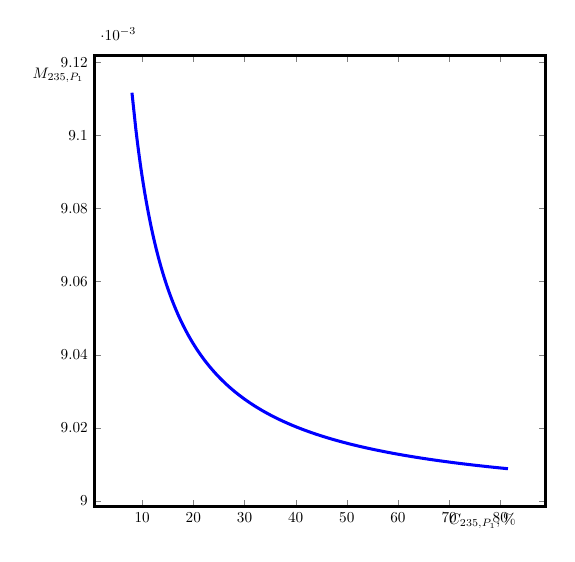
\begin{tikzpicture}[,
scale=0.55]
\begin{axis}[
  xlabel style = {{at={(axis description cs:.86,0)}}},
  ylabel = {$M_{235,P_1}$},
  ylabel style = {{at={(axis description cs:-0.08,.925)},rotate=270,anchor=south}},
  xlabel = {$C_{235,P_1}, \%$},
  width=12cm, height=12cm, line width=2pt
]

\addplot+[
  mark = {none}
] coordinates {
  (8.0, 0.009111645553414241)
  (8.75, 0.0091017702125065)
  (9.0, 0.009098848295071484)
  (9.25, 0.009096086045214)
  (9.5, 0.009093470723500143)
  (9.75, 0.009090990910644607)
  (10.0, 0.00908863634082525)
  (10.25, 0.009086397759630997)
  (10.5, 0.009084266802498001)
  (10.75, 0.009082235890267501)
  (11.0, 0.00908029813911642)
  (11.25, 0.009078447282604948)
  (11.5, 0.009076677603981013)
  (11.75, 0.009074983877200895)
  (12.0, 0.009073361315384259)
  (12.25, 0.00907180552563272)
  (12.5, 0.009070312469313927)
  (12.75, 0.009068878458541407)
  (13.0, 0.009067500000042155)
  (13.25, 0.009066173954411696)
  (13.5, 0.00906489728787538)
  (13.750000000000002, 0.009063667581395724)
  (14.000000000000002, 0.009062482014421195)
  (14.249999999999998, 0.009061338339251261)
  (14.499999999999998, 0.009060234375023613)
  (14.75, 0.009059168051505043)
  (15.0, 0.009058137545975231)
  (15.25, 0.00905714105051603)
  (15.5, 0.00905617690879367)
  (15.75, 0.009055243570310421)
  (16.0, 0.009054339582084164)
  (16.25, 0.00905346358110072)
  (16.5, 0.009052614287456559)
  (16.75, 0.009051790498119234)
  (17.0, 0.009050991081241673)
  (17.25, 0.00905021497097372)
  (17.5, 0.009049461162720995)
  (17.75, 0.009048728708806643)
  (18.0, 0.00904801671449666)
  (18.25, 0.009047324334353698)
  (18.5, 0.00904665076888807)
  (18.75, 0.009045995261478194)
  (19.0, 0.009045357095535361)
  (19.25, 0.009044735639730662)
  (19.5, 0.009044130154683458)
  (19.75, 0.009043540060440437)
  (20.0, 0.00904296481221043)
  (20.25, 0.009042403834595814)
  (20.5, 0.009041856609191412)
  (20.75, 0.00904132263216406)
  (21.0, 0.00904080143545228)
  (21.25, 0.009040292553237213)
  (21.5, 0.00903979550937721)
  (21.75, 0.009039309994501544)
  (22.0, 0.009038835564449479)
  (22.25, 0.009038371843888997)
  (22.5, 0.009037918474243971)
  (22.75, 0.009037475112769424)
  (23.0, 0.009037041431687414)
  (23.25, 0.009036617117378845)
  (23.5, 0.009036201869627142)
  (23.75, 0.009035795400909865)
  (24.0, 0.009035397435734786)
  (24.25, 0.009035007710017202)
  (24.5, 0.009034625970495555)
  (24.75, 0.00903425197418256)
  (25.0, 0.009033885487849455)
  (25.25, 0.009033526287540965)
  (25.5, 0.009033174158118945)
  (25.75, 0.009032828892832686)
  (26.0, 0.009032490292914117)
  (26.25, 0.009032158167196222)
  (26.5, 0.009031832331753151)
  (26.75, 0.009031512609560576)
  (27.0, 0.009031198830174978)
  (27.250000000000004, 0.009030890829430675)
  (27.500000000000004, 0.009030588449153424)
  (27.750000000000004, 0.009030291536889548)
  (28.000000000000004, 0.009029999945649653)
  (28.249999999999996, 0.009029713533665974)
  (28.499999999999996, 0.00902943216416257)
  (28.749999999999996, 0.009029155705137498)
  (28.999999999999996, 0.009028884029156364)
  (29.25, 0.009028617013156427)
  (29.5, 0.009028354538260753)
  (29.75, 0.009028096489601721)
  (30.0, 0.00902784275615345)
  (30.25, 0.009027593230572475)
  (30.5, 0.009027347809046375)
  (30.75, 0.009027106391149743)
  (31.0, 0.00902686887970717)
  (31.25, 0.009026635180662839)
  (31.5, 0.009026405202956339)
  (31.75, 0.009026178858404345)
  (32.0, 0.009025956061587903)
  (32.25, 0.009025736729744938)
  (32.5, 0.009025520782667745)
  (32.75, 0.009025308142605212)
  (33.0, 0.009025098734169474)
  (33.25, 0.009024892484246807)
  (33.5, 0.009024689321912506)
  (33.75, 0.009024489178349589)
  (34.0, 0.009024291986771057)
  (34.25, 0.009024097682345614)
  (34.5, 0.009023906202126574)
  (34.75, 0.009023717484983906)
  (35.0, 0.009023531471539137)
  (35.25, 0.009023348104103083)
  (35.5, 0.009023167326616195)
  (35.75, 0.009022989084591409)
  (36.0, 0.009022813325059406)
  (36.25, 0.009022639996516136)
  (36.5, 0.009022469048872474)
  (36.75, 0.009022300433405987)
  (37.0, 0.009022134102714624)
  (37.25, 0.0090219700106723)
  (37.5, 0.009021808112386228)
  (37.75, 0.009021648364155999)
  (38.0, 0.009021490723434238)
  (38.25, 0.009021335148788823)
  (38.5, 0.009021181599866602)
  (38.75, 0.009021030037358468)
  (39.0, 0.009020880422965822)
  (39.25, 0.009020732719368324)
  (39.5, 0.009020586890192831)
  (39.75, 0.00902044289998355)
  (40.0, 0.009020300714173297)
  (40.25, 0.009020160295716685)
  (40.5, 0.009020021613513425)
  (40.75, 0.009019884636650533)
  (41.0, 0.009019749333815445)
  (41.25, 0.009019615674453465)
  (41.5, 0.009019483628744707)
  (41.75, 0.009019353167581854)
  (42.0, 0.009019224262548657)
  (42.25, 0.009019096885899256)
  (42.5, 0.009018971010538156)
  (42.75, 0.009018846610000958)
  (43.0, 0.009018723658435686)
  (43.25, 0.009018602130584792)
  (43.5, 0.009018482001767763)
  (43.75, 0.009018363247864284)
  (44.0, 0.00901824584529798)
  (44.25, 0.009018129771020695)
  (44.5, 0.009018015002497262)
  (44.75, 0.00901790151769078)
  (45.0, 0.009017789295048354)
  (45.25, 0.009017678313487286)
  (45.5, 0.009017568552381682)
  (45.75, 0.009017459991549497)
  (46.0, 0.009017352611239942)
  (46.25, 0.009017246392121295)
  (46.5, 0.00901714131526906)
  (46.75, 0.009017037362154458)
  (47.0, 0.009016934514633253)
  (47.25, 0.009016832754934914)
  (47.5, 0.009016732065652023)
  (47.75, 0.009016633001095729)
  (48.0, 0.009016534446810474)
  (48.25, 0.009016436915934194)
  (48.5, 0.009016340392608286)
  (48.75, 0.009016244861300112)
  (49.0, 0.009016150306794668)
  (49.25, 0.009016056714186524)
  (49.5, 0.009015964068871979)
  (49.75, 0.009015872356541454)
  (50.0, 0.009015781563172147)
  (50.24999999999999, 0.00901569167502086)
  (50.5, 0.009015602678617089)
  (50.74999999999999, 0.009015514560756284)
  (51.0, 0.009015427308493298)
  (51.24999999999999, 0.009015340909136091)
  (51.5, 0.009015255350239526)
  (51.74999999999999, 0.009015170619599432)
  (52.0, 0.009015086705246778)
  (52.25, 0.009015003595442049)
  (52.5, 0.009014921278669761)
  (52.75, 0.00901483974363315)
  (53.0, 0.009014758979249004)
  (53.25, 0.009014678974642627)
  (53.5, 0.009014599719142978)
  (53.75, 0.009014521202277909)
  (54.0, 0.009014443413769559)
  (54.25, 0.009014366343529881)
  (54.50000000000001, 0.00901428998165625)
  (54.75, 0.009014214318427251)
  (55.00000000000001, 0.00901413934429854)
  (55.25, 0.009014065049898833)
  (55.50000000000001, 0.009013991426025996)
  (55.75, 0.009013918463643251)
  (56.00000000000001, 0.009013846153875479)
  (56.25, 0.009013774488005614)
  (56.49999999999999, 0.00901370345747114)
  (56.75, 0.009013633053860692)
  (56.99999999999999, 0.009013563268910726)
  (57.25, 0.009013494094502271)
  (57.49999999999999, 0.009013425522657811)
  (57.75, 0.00901335754553819)
  (57.99999999999999, 0.009013290155439639)
  (58.25, 0.009013223344790855)
  (58.5, 0.00901315710615017)
  (58.75, 0.009013091432202788)
  (59.0, 0.009013026315758083)
  (59.25, 0.00901296174974698)
  (59.5, 0.009012897727219393)
  (59.75, 0.009012834241341723)
  (60.0, 0.009012771285394442)
  (60.25, 0.009012708852769698)
  (60.5, 0.00901264693696901)
  (60.75000000000001, 0.009012585531601018)
  (61.0, 0.00901252463037926)
  (61.25000000000001, 0.009012464227120046)
  (61.5, 0.009012404315740343)
  (61.75000000000001, 0.009012344890255737)
  (62.0, 0.009012285944778433)
  (62.25000000000001, 0.009012227473515303)
  (62.5, 0.009012169470765989)
  (62.74999999999999, 0.009012111930921026)
  (63.0, 0.009012054848460052)
  (63.24999999999999, 0.00901199821795001)
  (63.5, 0.009011942034043426)
  (63.74999999999999, 0.009011886291476714)
  (64.0, 0.009011830985068525)
  (64.25, 0.009011776109718119)
  (64.5, 0.009011721660403788)
  (64.75, 0.009011667632181317)
  (65.0, 0.009011614020182456)
  (65.25, 0.009011560819613454)
  (65.5, 0.009011508025753606)
  (65.75, 0.00901145563395382)
  (66.0, 0.009011403639635264)
  (66.25, 0.009011352038287967)
  (66.5, 0.009011300825469516)
  (66.75, 0.00901124999680374)
  (67.0, 0.009011199547979423)
  (67.25, 0.00901114947474907)
  (67.5, 0.009011099772927661)
  (67.75, 0.009011050438391446)
  (68.0, 0.009011001467076764)
  (68.25, 0.00901095285497887)
  (68.5, 0.0090109045981508)
  (68.75, 0.009010856692702247)
  (69.0, 0.00901080913479844)
  (69.25, 0.009010761920659067)
  (69.5, 0.009010715046557203)
  (69.75, 0.009010668508818246)
  (70.0, 0.009010622303818869)
  (70.25, 0.00901057642798601)
  (70.5, 0.009010530877795835)
  (70.75, 0.00901048564977274)
  (71.0, 0.009010440740488368)
  (71.25, 0.009010396146560597)
  (71.5, 0.009010351864652596)
  (71.75, 0.009010307891471833)
  (72.0, 0.009010264223769117)
  (72.25, 0.009010220858337654)
  (72.5, 0.009010177792012079)
  (72.75, 0.00901013502166751)
  (73.0, 0.00901009254421861)
  (73.25, 0.009010050356618626)
  (73.5, 0.009010008455858446)
  (73.75, 0.009009966838965653)
  (74.0, 0.009009925503003568)
  (74.25, 0.009009884445070285)
  (74.5, 0.009009843662297713)
  (74.75, 0.009009803151850605)
  (75.0, 0.009009762910925562)
  (75.25, 0.00900972293675004)
  (75.5, 0.009009683226581354)
  (75.75, 0.009009643777705635)
  (76.0, 0.009009604587436796)
  (76.25, 0.009009565653115467)
  (76.5, 0.009009526972107914)
  (76.75, 0.00900948854180492)
  (77.0, 0.009009450359620655)
  (77.25, 0.009009412422991511)
  (77.5, 0.0090093747293749)
  (77.75, 0.009009337276248005)
  (78.0, 0.009009300061106531)
  (78.25, 0.009009263431930687)
  (78.5, 0.009009226717816872)
  (78.75, 0.009009190241608116)
  (79.0, 0.009009153717338046)
  (79.25, 0.009009117547127953)
  (79.5, 0.009009081533171134)
  (79.75, 0.009009046608607772)
  (80.0, 0.009009011263082943)
  (80.25, 0.009008976130382018)
  (80.5, 0.009008941231325876)
  (80.75, 0.009008905699671515)
  (81.0, 0.009008871149798441)
  (81.25, 0.009008836806363333)
  (81.5, 0.009008802666955288)
};

\end{axis}
\end{tikzpicture}

}
%     \caption{{Зависимость массы $^{235}$U в потоке обогащенной фракции первого каскада $P_1$ от концентрации $^{235}$U в потоке легкой фракции первого каскада{\label{M235P1}}}}
% \end{figure}



% \begin{figure}
%     \centering
%     \begin{minipage}{.5\textwidth}
%       \centering
%       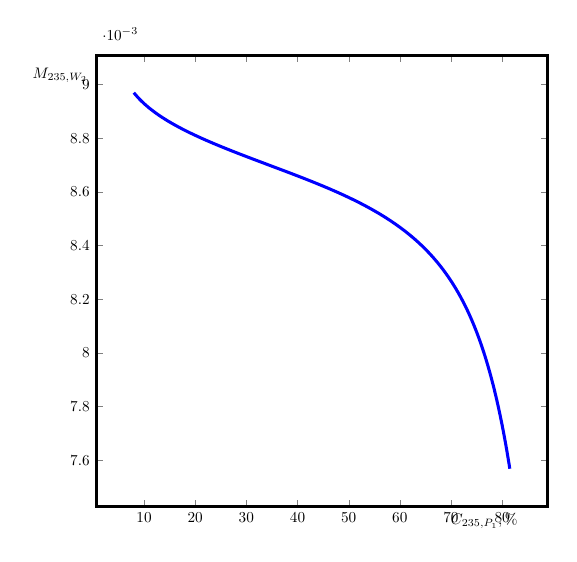
\begin{tikzpicture}[,
scale=0.55]
\begin{axis}[
  xlabel style = {{at={(axis description cs:.86,0)}}},
  ylabel = {$M_{235,W_2}$},
  ylabel style = {{at={(axis description cs:-0.08,.925)},rotate=270,anchor=south}},
  xlabel = {$C_{235,P_1}, \%$},
  width=12cm, height=12cm, line width=2pt
]

\addplot+[
  mark = {none}
] coordinates {
  (8.0, 0.008969582934887354)
  (8.75, 0.008953050957470687)
  (9.0, 0.008947961457989935)
  (9.25, 0.008943055236043482)
  (9.5, 0.008938318351511982)
  (9.75, 0.008933738550573236)
  (10.0, 0.008929304579336527)
  (10.25, 0.00892500600276735)
  (10.5, 0.008920834068883481)
  (10.75, 0.008916780111045451)
  (11.0, 0.008912836522459945)
  (11.25, 0.00890899638778039)
  (11.5, 0.008905253328491191)
  (11.75, 0.00890160156292447)
  (12.0, 0.008898035595833407)
  (12.25, 0.008894550529189556)
  (12.5, 0.008891142055842764)
  (12.75, 0.008887805346784065)
  (13.0, 0.00888453702453666)
  (13.25, 0.00888133327101651)
  (13.5, 0.008878190722767425)
  (13.750000000000002, 0.008875106482081157)
  (14.000000000000002, 0.008872077308430648)
  (14.249999999999998, 0.008869100608211533)
  (14.499999999999998, 0.008866173925463825)
  (14.75, 0.008863294824375137)
  (15.0, 0.00886046103386761)
  (15.25, 0.008857670643016527)
  (15.5, 0.0088549215481551)
  (15.75, 0.008852211964820795)
  (16.0, 0.008849540023391618)
  (16.25, 0.00884690431436794)
  (16.5, 0.008844303237468832)
  (16.75, 0.008841735275167406)
  (17.0, 0.008839199039822518)
  (17.25, 0.008836693480195931)
  (17.5, 0.00883421697699065)
  (17.75, 0.0088317687332981)
  (18.0, 0.00882934748342718)
  (18.25, 0.00882695214685525)
  (18.5, 0.008824581764264412)
  (18.75, 0.008822235354809235)
  (19.0, 0.008819912216795097)
  (19.25, 0.00881761123796545)
  (19.5, 0.008815331753722773)
  (19.75, 0.00881307281029624)
  (20.0, 0.008810833888339926)
  (20.25, 0.008808614074903603)
  (20.5, 0.008806412834731561)
  (20.75, 0.008804229443483637)
  (21.0, 0.008802063270662694)
  (21.25, 0.008799913744817398)
  (21.5, 0.00879778027046047)
  (21.75, 0.008795662265158915)
  (22.0, 0.008793559276179001)
  (22.25, 0.00879147051686481)
  (22.5, 0.008789395993835127)
  (22.75, 0.008787334812847844)
  (23.0, 0.008785286700981111)
  (23.25, 0.008783251073485748)
  (23.5, 0.008781227661490464)
  (23.75, 0.008779215933748342)
  (24.0, 0.008777215454272918)
  (24.25, 0.008775225876559527)
  (24.5, 0.008773246979830614)
  (24.75, 0.008771278510945961)
  (25.0, 0.008769319200942987)
  (25.25, 0.008767369764545823)
  (25.5, 0.008765429352778268)
  (25.75, 0.008763497724964686)
  (26.0, 0.00876157460680785)
  (26.25, 0.008759659733538669)
  (26.5, 0.008757752721138398)
  (26.75, 0.008755853183943181)
  (27.0, 0.008753960981176848)
  (27.250000000000004, 0.008752075704564152)
  (27.500000000000004, 0.008750197251064693)
  (27.750000000000004, 0.008748325098700112)
  (28.000000000000004, 0.008746459143606207)
  (28.249999999999996, 0.008744599156599683)
  (28.499999999999996, 0.00874274475756152)
  (28.749999999999996, 0.00874089570432083)
  (28.999999999999996, 0.008739051758361226)
  (29.25, 0.008737212859217611)
  (29.5, 0.008735378568265433)
  (29.75, 0.008733548658001515)
  (30.0, 0.008731722851187139)
  (30.25, 0.008729901060330605)
  (30.5, 0.008728082992807404)
  (30.75, 0.008726268277156625)
  (31.0, 0.008724456956166039)
  (31.25, 0.008722648537674339)
  (31.5, 0.00872084298824132)
  (31.75, 0.008719039917813124)
  (32.0, 0.008717239389980553)
  (32.25, 0.008715440946923838)
  (32.5, 0.008713644358357074)
  (32.75, 0.008711849635932507)
  (33.0, 0.00871005612709628)
  (33.25, 0.008708264214899087)
  (33.5, 0.00870647327897643)
  (33.75, 0.008704683167840163)
  (34.0, 0.008702893749631745)
  (34.25, 0.008701104753714752)
  (34.5, 0.008699315918146305)
  (34.75, 0.008697527280060588)
  (35.0, 0.008695738295444984)
  (35.25, 0.008693949011086596)
  (35.5, 0.008692159067325417)
  (35.75, 0.008690368279467689)
  (36.0, 0.008688576444007815)
  (36.25, 0.008686783394698666)
  (36.5, 0.008684988871695434)
  (36.75, 0.008683192626879025)
  (37.0, 0.008681394560566527)
  (37.25, 0.008679594405661325)
  (37.5, 0.008677791839637863)
  (37.75, 0.00867598678009571)
  (38.0, 0.008674178926183503)
  (38.25, 0.008672368153057894)
  (38.5, 0.008670554088754482)
  (38.75, 0.0086687365946658)
  (39.0, 0.008666915421462824)
  (39.25, 0.008665090385095373)
  (39.5, 0.008663261262198822)
  (39.75, 0.008661427825532907)
  (40.0, 0.008659589749934544)
  (40.25, 0.008657746844634986)
  (40.5, 0.008655898846421654)
  (40.75, 0.00865404564337099)
  (41.0, 0.008652186658828356)
  (41.25, 0.008650322200803322)
  (41.5, 0.008648451545630592)
  (41.75, 0.008646574533356776)
  (42.0, 0.008644690955891309)
  (42.25, 0.008642800636894704)
  (42.5, 0.008640903224070825)
  (42.75, 0.00863899844671149)
  (43.0, 0.008637085957510716)
  (43.25, 0.00863516575727924)
  (43.5, 0.008633237218089401)
  (43.75, 0.008631300408230349)
  (44.0, 0.008629354764905747)
  (44.25, 0.008627400106242656)
  (44.5, 0.008625436177556048)
  (44.75, 0.0086234625877378)
  (45.0, 0.00862147908941806)
  (45.25, 0.008619485381956294)
  (45.5, 0.008617481036809113)
  (45.75, 0.008615465921339726)
  (46.0, 0.008613439478955834)
  (46.25, 0.008611401795773408)
  (46.5, 0.008609352102023984)
  (46.75, 0.008607290031975672)
  (47.0, 0.008605215642082472)
  (47.25, 0.008603128259590765)
  (47.5, 0.008601027675848224)
  (47.75, 0.008598913983259165)
  (48.0, 0.008596785691386668)
  (48.25, 0.008594643293756862)
  (48.5, 0.008592485759095589)
  (48.75, 0.008590313355086041)
  (49.0, 0.0085881251954436)
  (49.25, 0.008585921074581795)
  (49.5, 0.008583700611067892)
  (49.75, 0.008581463263063322)
  (50.0, 0.008579208603379272)
  (50.24999999999999, 0.008576936252814263)
  (50.5, 0.008574645722361236)
  (50.74999999999999, 0.008572336531763418)
  (51.0, 0.008570008133297382)
  (51.24999999999999, 0.00856766010981354)
  (51.5, 0.008565291973522108)
  (51.74999999999999, 0.008562903220451633)
  (52.0, 0.008560493278454286)
  (52.25, 0.00855806152083667)
  (52.5, 0.0085556076484768)
  (52.75, 0.008553130961714709)
  (53.0, 0.008550630846209386)
  (53.25, 0.00854810706771584)
  (53.5, 0.00854555774925702)
  (53.75, 0.0085429838369619)
  (54.0, 0.008540383924706487)
  (54.25, 0.008537757588306388)
  (54.50000000000001, 0.008535104091081134)
  (54.75, 0.008532422651702221)
  (55.00000000000001, 0.008529712611513763)
  (55.25, 0.008526973112919355)
  (55.50000000000001, 0.008524203723571044)
  (55.75, 0.008521403545945452)
  (56.00000000000001, 0.008518571606366723)
  (56.25, 0.00851570727763321)
  (56.49999999999999, 0.008512809808569574)
  (56.75, 0.008509878155889035)
  (56.99999999999999, 0.008506911456068385)
  (57.25, 0.008503908792779345)
  (57.49999999999999, 0.00850086938251702)
  (57.75, 0.008497792179323343)
  (57.99999999999999, 0.008494676202933862)
  (58.25, 0.008491520141475806)
  (58.5, 0.008488323553930758)
  (58.75, 0.008485084979440822)
  (59.0, 0.008481803250545655)
  (59.25, 0.008478477351644427)
  (59.5, 0.008475105879196487)
  (59.75, 0.008471688048711791)
  (60.0, 0.008468222192560626)
  (60.25, 0.008464707099481916)
  (60.5, 0.00846114133577974)
  (60.75000000000001, 0.008457523922427972)
  (61.0, 0.008453852639556711)
  (61.25000000000001, 0.00845012688494179)
  (61.5, 0.008446344688200533)
  (61.75000000000001, 0.008442504246032677)
  (62.0, 0.008438604167544233)
  (62.25000000000001, 0.008434642701742214)
  (62.5, 0.00843061819667875)
  (62.74999999999999, 0.008426528551434788)
  (63.0, 0.008422371991251038)
  (63.24999999999999, 0.008418146665359498)
  (63.5, 0.008413850388432755)
  (63.74999999999999, 0.008409481193270963)
  (64.0, 0.00840503667489769)
  (64.25, 0.008400514684896585)
  (64.5, 0.00839591280165317)
  (64.75, 0.008391228646229737)
  (65.0, 0.008386459646753221)
  (65.25, 0.008381602891968784)
  (65.5, 0.008376656246177845)
  (65.75, 0.008371616339520984)
  (66.0, 0.008366480231628762)
  (66.25, 0.008361245162791847)
  (66.5, 0.008355907301054039)
  (66.75, 0.00835046404896195)
  (67.0, 0.008344911421099945)
  (67.25, 0.008339246074549682)
  (67.5, 0.008333463823960592)
  (67.75, 0.008327561384019997)
  (68.0, 0.008321533879538923)
  (68.25, 0.00831537758511544)
  (68.5, 0.00830908814223659)
  (68.75, 0.008302660204893444)
  (69.0, 0.008296089646192446)
  (69.25, 0.00828937113819764)
  (69.5, 0.008282499224605326)
  (69.75, 0.008275468531667402)
  (70.0, 0.00826827347415231)
  (70.25, 0.008260908009095722)
  (70.5, 0.00825336596088543)
  (70.75, 0.008245640203393603)
  (71.0, 0.008237724568319199)
  (71.25, 0.00822961154384384)
  (71.5, 0.008221293669866929)
  (71.75, 0.00821276338124383)
  (72.0, 0.008204012187817605)
  (72.25, 0.00819503168306494)
  (72.5, 0.008185813088394164)
  (72.75, 0.008176346645735303)
  (73.0, 0.00816662305461966)
  (73.25, 0.008156631890100853)
  (73.5, 0.008146362682047308)
  (73.75, 0.008135803206441633)
  (74.0, 0.008124942750070615)
  (74.25, 0.008113768797907307)
  (74.5, 0.008102268366638297)
  (74.75, 0.00809042809718903)
  (75.0, 0.008078233643784233)
  (75.25, 0.008065670407119764)
  (75.5, 0.008052722827568548)
  (75.75, 0.008039374511333873)
  (76.0, 0.00802560836493737)
  (76.25, 0.008011406404869104)
  (76.5, 0.007996750206473837)
  (76.75, 0.00798161953598353)
  (77.0, 0.007965994104478175)
  (77.25, 0.007949851853015227)
  (77.5, 0.007933169944668625)
  (77.75, 0.007915923760480153)
  (78.0, 0.007898088701745708)
  (78.25, 0.007879637419106009)
  (78.5, 0.00786054173728438)
  (78.75, 0.007840771975822277)
  (79.0, 0.00782029584895143)
  (79.25, 0.0077990811576082175)
  (79.5, 0.007777091914924569)
  (79.75, 0.00775429154132833)
  (80.0, 0.007730640361314449)
  (80.25, 0.007706093308217856)
  (80.5, 0.00768060886945932)
  (80.75, 0.007654137404335572)
  (81.0, 0.007626629210857389)
  (81.25, 0.007598029377462495)
  (81.5, 0.00756827981297914)
};

\end{axis}
\end{tikzpicture}


% \caption{{Зависимость массы $^{235}$U в потоке тяжелой фракции второго каскада $W_2$ от концентрации $^{235}$U в потоке легкой фракции первого каскада{\label{M235W2}}}}
%     \end{minipage}%
%     \begin{minipage}{.5\textwidth}
%       \centering
%       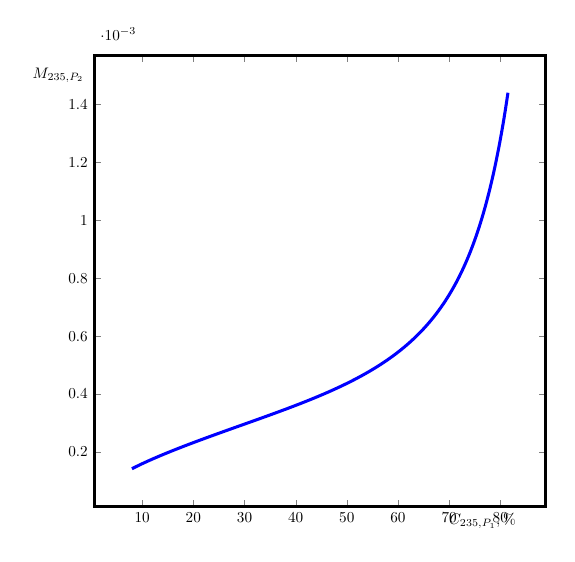
\begin{tikzpicture}[,
scale=0.55]
\begin{axis}[
  xlabel style = {{at={(axis description cs:.86,0)}}},
  ylabel = {$M_{235,P_2}$},
  ylabel style = {{at={(axis description cs:-0.08,.925)},rotate=270,anchor=south}},
  xlabel = {$C_{235,P_1}, \%$},
  width=12cm, height=12cm, line width=2pt
]

\addplot+[
  mark = {none}
] coordinates {
  (8.0, 0.00014206261852688643)
  (8.75, 0.0001487192550358152)
  (9.0, 0.00015088683708154766)
  (9.25, 0.00015303080917051723)
  (9.5, 0.0001551523719881621)
  (9.75, 0.00015725236007136956)
  (10.0, 0.0001593317614887236)
  (10.25, 0.00016139175686364607)
  (10.5, 0.00016343273361451926)
  (10.75, 0.0001654557792220484)
  (11.0, 0.0001674616166564755)
  (11.25, 0.00016945089482455766)
  (11.5, 0.00017142427548982213)
  (11.75, 0.00017338231427642395)
  (12.0, 0.00017532571955085064)
  (12.25, 0.00017725499644316329)
  (12.5, 0.00017917041347116197)
  (12.75, 0.00018107311175734472)
  (13.0, 0.00018296297550549672)
  (13.25, 0.00018484068339518633)
  (13.5, 0.00018670656510795378)
  (13.750000000000002, 0.00018856109931456714)
  (14.000000000000002, 0.00019040470599054806)
  (14.249999999999998, 0.00019223773103972837)
  (14.499999999999998, 0.00019406044955978683)
  (14.75, 0.00019587322712990587)
  (15.0, 0.00019767651210762089)
  (15.25, 0.00019947040749950323)
  (15.5, 0.0002012553606385691)
  (15.75, 0.000203031605489627)
  (16.0, 0.0002047995586925459)
  (16.25, 0.00020655926673278035)
  (16.5, 0.00020831104998772658)
  (16.75, 0.00021005522295182956)
  (17.0, 0.00021179204141915403)
  (17.25, 0.00021352149077778944)
  (17.5, 0.00021524418573034358)
  (17.75, 0.00021695997550854248)
  (18.0, 0.00021866923106948102)
  (18.25, 0.00022037218749844817)
  (18.5, 0.0002220690046236574)
  (18.75, 0.00022375990666895904)
  (19.0, 0.00022544487874026487)
  (19.25, 0.00022712440176520985)
  (19.5, 0.000228798400960687)
  (19.75, 0.0002304672501441958)
  (20.0, 0.00023213092387050163)
  (20.25, 0.00023378975969221073)
  (20.5, 0.00023544377445984787)
  (20.75, 0.00023709318868042308)
  (21.0, 0.00023873816478958473)
  (21.25, 0.00024037880841981435)
  (21.5, 0.0002420152389167409)
  (21.75, 0.0002436477293426275)
  (22.0, 0.00024527628827047715)
  (22.25, 0.00024690132702418757)
  (22.5, 0.000248522480408844)
  (22.75, 0.0002501402999215804)
  (23.0, 0.00025175473070630355)
  (23.25, 0.00025336604389309693)
  (23.5, 0.00025497420813668046)
  (23.75, 0.0002565794671615227)
  (24.0, 0.00025818198146186926)
  (24.25, 0.00025978183345767603)
  (24.5, 0.00026137899066494216)
  (24.75, 0.00026297346323659904)
  (25.0, 0.00026456628690646705)
  (25.25, 0.0002661565229951418)
  (25.5, 0.0002677448053406744)
  (25.75, 0.000269331167867999)
  (26.0, 0.0002709156861062661)
  (26.25, 0.00027249843365755483)
  (26.5, 0.0002740796106147544)
  (26.75, 0.00027565942561739483)
  (27.0, 0.00027723784899813124)
  (27.250000000000004, 0.0002788151248665254)
  (27.500000000000004, 0.0002803911980887289)
  (27.750000000000004, 0.0002819664381894382)
  (28.000000000000004, 0.00028354080204344467)
  (28.249999999999996, 0.00028511437706629176)
  (28.499999999999996, 0.0002866874066010505)
  (28.749999999999996, 0.00028826000081666806)
  (28.999999999999996, 0.00028983227079514023)
  (29.25, 0.00029140415393881665)
  (29.5, 0.00029297596999531867)
  (29.75, 0.0002945478316002078)
  (30.0, 0.00029611990496630937)
  (30.25, 0.0002976921702418694)
  (30.5, 0.00029926481623896936)
  (30.75, 0.00030083811399311594)
  (31.0, 0.0003024119235411315)
  (31.25, 0.0003039866429885015)
  (31.5, 0.00030556221471501877)
  (31.75, 0.0003071389405912217)
  (32.0, 0.00030871667160734965)
  (32.25, 0.0003102957828210971)
  (32.5, 0.00031187642431066976)
  (32.75, 0.00031345850667270484)
  (33.0, 0.0003150426070731949)
  (33.25, 0.0003166282693477201)
  (33.5, 0.00031821604293607675)
  (33.75, 0.00031980601050942775)
  (34.0, 0.0003213982371393116)
  (34.25, 0.00032299292863086315)
  (34.5, 0.00032459028398027255)
  (34.75, 0.0003261902049233192)
  (35.0, 0.0003277931760941529)
  (35.25, 0.0003293990930164905)
  (35.5, 0.0003310082592907783)
  (35.75, 0.00033262080512371883)
  (36.0, 0.0003342368810515949)
  (36.25, 0.00033585660181746966)
  (36.5, 0.0003374801771770407)
  (36.75, 0.00033910780652696257)
  (37.0, 0.0003407395421480962)
  (37.25, 0.0003423756050109775)
  (37.5, 0.0003440162727483667)
  (37.75, 0.0003456615840602884)
  (38.0, 0.00034731179725073575)
  (38.25, 0.00034896699573092933)
  (38.5, 0.0003506275111121188)
  (38.75, 0.0003522934426926643)
  (39.0, 0.00035396500150299795)
  (39.25, 0.0003556423342729505)
  (39.5, 0.0003573256279940082)
  (39.75, 0.00035901507445064196)
  (40.0, 0.0003607109642387537)
  (40.25, 0.0003624134510816995)
  (40.5, 0.00036412276709177246)
  (40.75, 0.0003658389932795444)
  (41.0, 0.0003675626749870876)
  (41.25, 0.00036929347365014225)
  (41.5, 0.00037103208311411453)
  (41.75, 0.00037277863422507766)
  (42.0, 0.00037453330665735036)
  (42.25, 0.0003762962490045512)
  (42.5, 0.00037806778646733223)
  (42.75, 0.00037984816328946784)
  (43.0, 0.0003816377009249703)
  (43.25, 0.00038343637330555364)
  (43.5, 0.0003852447836783621)
  (43.75, 0.0003870628396339368)
  (44.0, 0.0003888910803922337)
  (44.25, 0.00039072966477804054)
  (44.5, 0.0003925788249412114)
  (44.75, 0.0003944389299529779)
  (45.0, 0.000396310205630296)
  (45.25, 0.00039819293153099146)
  (45.5, 0.00040008751557256785)
  (45.75, 0.00040199407020977)
  (46.0, 0.00040391313228410814)
  (46.25, 0.0004058445963478875)
  (46.5, 0.000407789213245078)
  (46.75, 0.00040974733017878527)
  (47.0, 0.00041171887255078395)
  (47.25, 0.00041370449534414876)
  (47.5, 0.00041570438980380016)
  (47.75, 0.0004177190178365665)
  (48.0, 0.00041974875542380533)
  (48.25, 0.00042179362217733245)
  (48.5, 0.00042385463351269574)
  (48.75, 0.0004259315062140724)
  (49.0, 0.00042802511135106775)
  (49.25, 0.0004301356396047288)
  (49.5, 0.0004322634578040857)
  (49.75, 0.00043440909347813053)
  (50.0, 0.0004365729597928729)
  (50.24999999999999, 0.00043875542220659535)
  (50.5, 0.00044095695625585315)
  (50.74999999999999, 0.0004431780289928668)
  (51.0, 0.00044541917519591665)
  (51.24999999999999, 0.00044768079932255096)
  (51.5, 0.0004499633767174201)
  (51.74999999999999, 0.0004522673991477988)
  (52.0, 0.00045459342679249256)
  (52.25, 0.00045694207460538074)
  (52.5, 0.00045931363019295965)
  (52.75, 0.0004617087819184397)
  (53.0, 0.0004641281330396219)
  (53.25, 0.00046657190692678724)
  (53.5, 0.0004690419698859583)
  (53.75, 0.00047153736531601004)
  (54.0, 0.00047405948906307284)
  (54.25, 0.00047660875522349496)
  (54.50000000000001, 0.0004791858905751159)
  (54.75, 0.00048179166672502986)
  (55.00000000000001, 0.00048442673278477555)
  (55.25, 0.00048709193697948)
  (55.50000000000001, 0.0004897877024549516)
  (55.75, 0.0004925149176977991)
  (56.00000000000001, 0.0004952745475087547)
  (56.25, 0.000498067210372404)
  (56.49999999999999, 0.0005008936489015665)
  (56.75, 0.0005037548979716578)
  (56.99999999999999, 0.0005066518128423399)
  (57.25, 0.0005095853017229255)
  (57.49999999999999, 0.0005125561401407897)
  (57.75, 0.0005155653662148463)
  (57.99999999999999, 0.0005186139525057761)
  (58.25, 0.0005217032033150501)
  (58.5, 0.0005248335522194126)
  (58.75, 0.0005280064527619661)
  (59.0, 0.0005312230652124307)
  (59.25, 0.0005344843981025534)
  (59.5, 0.000537791848022905)
  (59.75, 0.0005411461926299319)
  (60.0, 0.0005445490928338145)
  (60.25, 0.0005480017532877826)
  (60.5, 0.0005515056011892717)
  (60.75000000000001, 0.0005550616091730453)
  (61.0, 0.0005586719908225494)
  (61.25000000000001, 0.0005623373421782563)
  (61.5, 0.0005660596275398105)
  (61.75000000000001, 0.0005698406442230616)
  (62.0, 0.0005736817772341985)
  (62.25000000000001, 0.0005775847717730899)
  (62.5, 0.0005815512740872374)
  (62.74999999999999, 0.000585583379486238)
  (63.0, 0.000589682857209016)
  (63.24999999999999, 0.0005938515525905125)
  (63.5, 0.0005980916456106702)
  (63.74999999999999, 0.00060240509820575)
  (64.0, 0.0006067943101708379)
  (64.25, 0.0006112614248215335)
  (64.5, 0.0006158088587506189)
  (64.75, 0.0006204389859515801)
  (65.0, 0.0006251543734292362)
  (65.25, 0.0006299579276446713)
  (65.5, 0.000634851779575759)
  (65.75, 0.0006398392944328368)
  (66.0, 0.0006449234080065024)
  (66.25, 0.0006501068754961208)
  (66.5, 0.0006553935244154773)
  (66.75, 0.0006607859478417916)
  (67.0, 0.0006662881268794789)
  (67.25, 0.0006719034001993863)
  (67.5, 0.0006776359489670697)
  (67.75, 0.0006834890543714472)
  (68.0, 0.0006894675875378399)
  (68.25, 0.000695575269863432)
  (68.5, 0.0007018164559142097)
  (68.75, 0.000708196487808803)
  (69.0, 0.0007147194886059934)
  (69.25, 0.0007213907824614268)
  (69.5, 0.0007282158219518746)
  (69.75, 0.0007351999771508405)
  (70.0, 0.0007423488296665546)
  (70.25, 0.0007496684188902872)
  (70.5, 0.0007571649169104045)
  (70.75, 0.0007648454463791348)
  (71.0, 0.0007727161721691653)
  (71.25, 0.0007807846027167577)
  (71.5, 0.0007890581947856685)
  (71.75, 0.0007975445102280024)
  (72.0, 0.0008062520359515104)
  (72.25, 0.000815189175272715)
  (72.5, 0.0008243647036179145)
  (72.75, 0.0008337883759322068)
  (73.0, 0.0008434694895989494)
  (73.25, 0.0008534184665177729)
  (73.5, 0.000863645773811138)
  (73.75, 0.0008741636325240199)
  (74.0, 0.0008849827529329532)
  (74.25, 0.0008961156471629762)
  (74.5, 0.0009075752956594171)
  (74.75, 0.0009193750546615769)
  (75.0, 0.0009315292671413294)
  (75.25, 0.0009440525296302777)
  (75.5, 0.0009569603990128037)
  (75.75, 0.0009702692663717642)
  (76.0, 0.000983996222499424)
  (76.25, 0.0009981592482463631)
  (76.5, 0.001012776765634078)
  (76.75, 0.0010278690058213892)
  (77.0, 0.0010434562551424789)
  (77.25, 0.0010595605699762838)
  (77.5, 0.0010762047847062738)
  (77.75, 0.0010934135157678515)
  (78.0, 0.0011112113593608204)
  (78.25, 0.0011296260128246794)
  (78.5, 0.0011486849805324923)
  (78.75, 0.0011684182657858363)
  (79.0, 0.0011888578683866158)
  (79.25, 0.001210036389519737)
  (79.5, 0.0012319896182465644)
  (79.75, 0.0012547550672794418)
  (80.0, 0.0012783709017684958)
  (80.25, 0.001302882822164161)
  (80.5, 0.0013283323618665562)
  (80.75, 0.0013547682953359422)
  (81.0, 0.0013822419389410525)
  (81.25, 0.0014108074289008383)
  (81.5, 0.0014405228539761475)
};

\end{axis}
\end{tikzpicture}


% \caption{{Зависимость массы $^{235}$U в потоке легкой фракции второго каскада $P_2$ от концентрации $^{235}$U в потоке легкой фракции первого каскада{\label{M235P2}}}}
% \end{minipage}
% \end{figure}





% \begin{figure}
%     \centering
%     \begin{minipage}{.5\textwidth}
%       \centering
%       \input{images/tex/loop_0.0495}
% \caption{{Зависимость массы $^{235}$U в потоке тяжелой фракции второго каскада $W_2$ от концентрации $^{235}$U в потоке легкой фракции первого каскада{\label{M235W2}}}}
%     \end{minipage}%
%     \begin{minipage}{.5\textwidth}
%       \centering
%       \input{images/tex/loop_0.0495}
% \caption{{Зависимость массы $^{235}$U в потоке легкой фракции второго каскада $P_2$ от концентрации $^{235}$U в потоке легкой фракции первого каскада{\label{M235P2}}}}
% \end{minipage}
% \end{figure}



% \clearpage


% \begin{figure}
%     \centerfloat{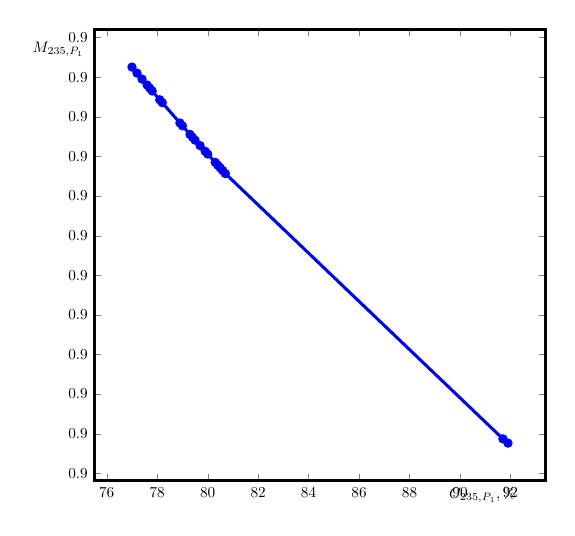
\begin{tikzpicture}[,
scale=0.55]
\begin{axis}[
  xlabel style = {{at={(axis description cs:.86,0)}}},
  ylabel = {$M_{235,P_1}$},
  ylabel style = {{at={(axis description cs:-0.08,.925)},rotate=270,anchor=south}},
  xlabel = {$C_{235,P_1}, \%$},
  width=12cm, height=12cm, line width=2pt
]

\addplot+ coordinates {
  (77.0, 0.9009450359620654)
  (77.2, 0.9009419990795269)
  (77.4, 0.9009389777821928)
  (77.60000000000001, 0.9009359719406014)
  (77.7, 0.9009344747754668)
  (77.8, 0.90093298142607)
  (78.10000000000001, 0.9009285241128198)
  (78.2, 0.9009270802954181)
  (78.9, 0.9009168234481284)
  (79.0, 0.9009153717338045)
  (79.3, 0.9009110332650255)
  (79.4, 0.9009095921620832)
  (79.5, 0.9009081533171134)
  (79.7, 0.9009053704589045)
  (79.9, 0.9009025375084988)
  (80.0, 0.9009011263082943)
  (80.30000000000001, 0.9008969131373471)
  (80.4, 0.9008955159491712)
  (80.5, 0.9008941231325875)
  (80.60000000000001, 0.9008927329166118)
  (80.7, 0.9008912634630402)
  (91.7, 0.9007572870913582)
  (91.9, 0.9007551470285345)
};


\end{axis}
\end{tikzpicture}

}
%     \caption{{Зависимость массы $^{235}$U в потоке обогащенной фракции первого каскада $P_1$ от концентрации $^{235}$U в потоке легкой фракции первого каскада{\label{M235P1}}}}
% \end{figure}



% \begin{figure}
%     \centering
%     \begin{minipage}{.5\textwidth}
%       \centering
%       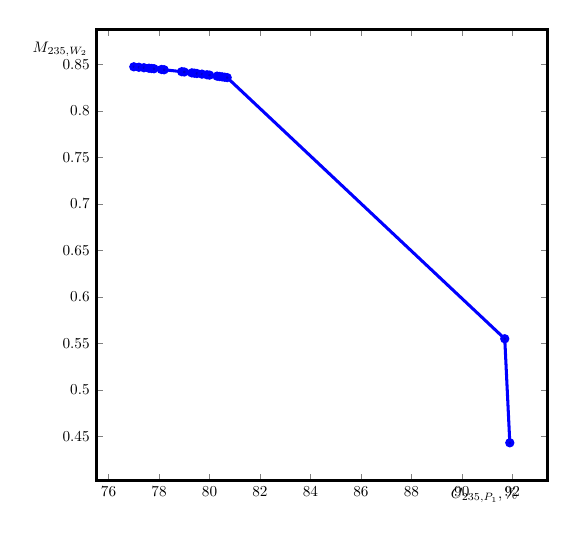
\begin{tikzpicture}[,
scale=0.55]
\begin{axis}[
  xlabel style = {{at={(axis description cs:.86,0)}}},
  ylabel = {$M_{235,W_2}$},
  ylabel style = {{at={(axis description cs:-0.08,.925)},rotate=270,anchor=south}},
  xlabel = {$C_{235,P_1}, \%$},
  width=12cm, height=12cm, line width=2pt
]

\addplot+ coordinates {
  (77.0, 0.847255489119533)
  (77.2, 0.8467603241080492)
  (77.4, 0.8462531188165721)
  (77.60000000000001, 0.8457329675283174)
  (77.7, 0.8454679156671182)
  (77.8, 0.8451994563533017)
  (78.10000000000001, 0.844373436959269)
  (78.2, 0.8440912014568814)
  (78.9, 0.8420078814549162)
  (79.0, 0.8416940899299918)
  (79.3, 0.8407279531588767)
  (79.4, 0.8403970353687986)
  (79.5, 0.8400617608739249)
  (79.7, 0.8393771028845441)
  (79.9, 0.8386732864869232)
  (80.0, 0.8383142216959854)
  (80.30000000000001, 0.8372059387814224)
  (80.4, 0.8368260037593748)
  (80.5, 0.8364406357319992)
  (80.60000000000001, 0.8360497907477974)
  (80.7, 0.8356532251113954)
  (91.7, 0.5548271981035123)
  (91.9, 0.44298000135762333)
};

\end{axis}
\end{tikzpicture}


% \caption{{Зависимость массы $^{235}$U в потоке тяжелой фракции второго каскада $W_2$ от концентрации $^{235}$U в потоке легкой фракции первого каскада{\label{M235W2}}}}
%     \end{minipage}%
%     \begin{minipage}{.5\textwidth}
%       \centering
%       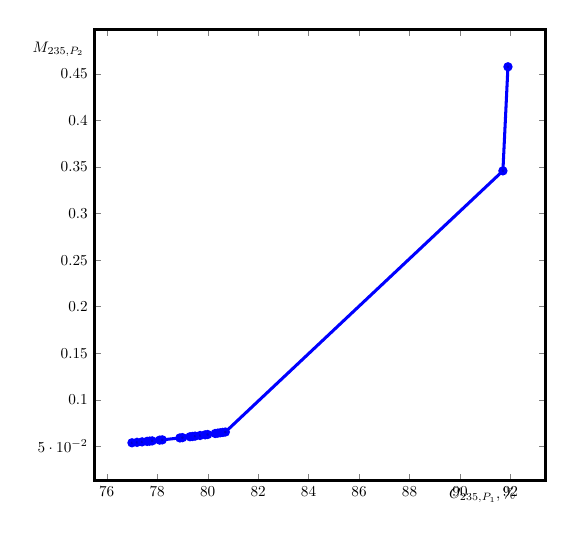
\begin{tikzpicture}[,
scale=0.55]
\begin{axis}[
  xlabel style = {{at={(axis description cs:.86,0)}}},
  ylabel = {$M_{235,P_2}$},
  ylabel style = {{at={(axis description cs:-0.08,.925)},rotate=270,anchor=south}},
  xlabel = {$C_{235,P_1}, \%$},
  width=12cm, height=12cm, line width=2pt
]

\addplot+ coordinates {
  (77.0, 0.05368954684253237)
  (77.2, 0.054181674971477814)
  (77.4, 0.054685858965620754)
  (77.60000000000001, 0.05520300441228407)
  (77.7, 0.0554665591083487)
  (77.8, 0.055733525072768485)
  (78.10000000000001, 0.05655508715355083)
  (78.2, 0.05683587883853662)
  (78.9, 0.058908941993212095)
  (79.0, 0.05922128180381264)
  (79.3, 0.06018308010614907)
  (79.4, 0.06051255679328454)
  (79.5, 0.060846392443188346)
  (79.7, 0.061528267574360626)
  (79.9, 0.06222925102157568)
  (80.0, 0.06258690461230906)
  (80.30000000000001, 0.06369097435592486)
  (80.4, 0.06406951218979642)
  (80.5, 0.06445348740058837)
  (80.60000000000001, 0.06484294216881445)
  (80.7, 0.06523803835164485)
  (91.7, 0.3459300889878457)
  (91.9, 0.4577751456709111)
};

\end{axis}
\end{tikzpicture}


% \caption{{Зависимость массы $^{235}$U в потоке легкой фракции второго каскада $P_2$ от концентрации $^{235}$U в потоке легкой фракции первого каскада{\label{M235P2}}}}
% \end{minipage}
% \end{figure}


% \begin{figure}
%     \centering
%     \begin{minipage}{.5\textwidth}
%       \centering
%       \begin{tikzpicture}[,
scale=0.55]
\begin{axis}[
  xlabel style = {{at={(axis description cs:.86,0)}}},
  ylabel = {$\textit{Потери РР}, \%$},
  ylabel style = {{at={(axis description cs:-0.13,.925)},rotate=270,anchor=south}},
  xlabel = {$C_{235,P_1}, \%$},
  width=12cm, height=12cm, line width=2pt
]

\addplot+ coordinates {
  (77.0, 13.181953313259436)
  (77.2, 13.217661797440005)
  (77.4, 13.253851411602069)
  (77.60000000000001, 13.290533396719301)
  (77.7, 13.309068077406137)
  (77.8, 13.327721487978986)
  (78.10000000000001, 13.38446777875146)
  (78.2, 13.40364934025208)
  (78.9, 13.541764785608363)
  (79.0, 13.562057422701635)
  (79.3, 13.623849319506029)
  (79.4, 13.644747270222124)
  (79.5, 13.665799543856917)
  (79.7, 13.708387512883169)
  (79.9, 13.75160756279821)
  (80.0, 13.773465106332289)
  (80.30000000000001, 13.840044982764322)
  (80.4, 13.862582937447154)
  (80.5, 13.885293367205396)
  (80.60000000000001, 13.908189489211376)
  (80.7, 13.931252115605178)
  (91.7, 22.774561853717792)
  (91.9, 25.642590663041908)
};

\end{axis}
\end{tikzpicture}


% \caption{{Зависимость перерасхода работы разделения от концентрации $^{235}$U в потоке легкой фракции первого каскада от концентрации $^{235}$U в потоке легкой фракции первого каскада{\label{SW_l}}}}
%     \end{minipage}%
%     \begin{minipage}{.5\textwidth}
%       \centering
%       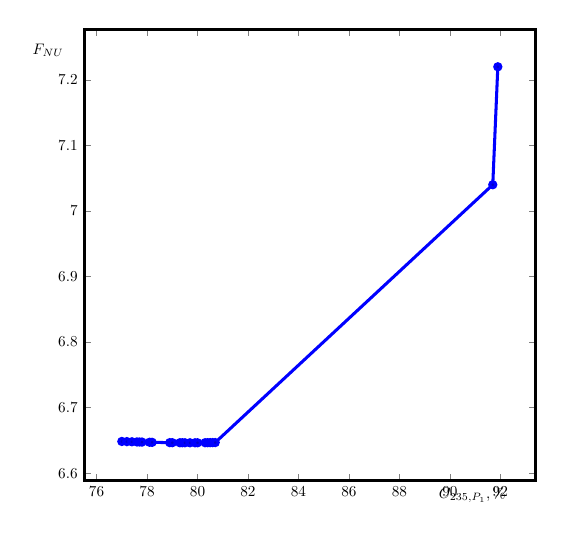
\begin{tikzpicture}[,
scale=0.55]
\begin{axis}[
  xlabel style = {{at={(axis description cs:.86,0)}}},
  ylabel = {$F_{NU}$},
  ylabel style = {{at={(axis description cs:-0.08,.925)},rotate=270,anchor=south}},
  xlabel = {$C_{235,P_1}, \%$},
  width=12cm, height=12cm, line width=2pt
]

\addplot+ coordinates {
  (77.0, 6.648369301601674)
  (77.2, 6.6481081422427755)
  (77.4, 6.6478609680670795)
  (77.60000000000001, 6.647628620667707)
  (77.7, 6.647518634806713)
  (77.8, 6.647412135764082)
  (78.10000000000001, 6.647118512130983)
  (78.2, 6.64702925961305)
  (78.9, 6.6465428786148735)
  (79.0, 6.646493966987278)
  (79.3, 6.646383406485429)
  (79.4, 6.646358460860561)
  (79.5, 6.646339791250357)
  (79.7, 6.646321811441468)
  (79.9, 6.646330897249658)
  (80.0, 6.646346113745254)
  (80.30000000000001, 6.64643598238657)
  (80.4, 6.646481376154359)
  (80.5, 6.646534553797508)
  (80.60000000000001, 6.646596419821)
  (80.7, 6.646666619197229)
  (91.7, 7.040023902346512)
  (91.9, 7.219931649864452)
};

\end{axis}
\end{tikzpicture}


% \caption{{Зависимость удельного расхода природного урана от концентрации $^{235}$U в потоке легкой фракции первого каскада от концентрации $^{235}$U в потоке легкой фракции первого каскада{\label{Fnu}}}}
% \end{minipage}
% \end{figure}


% \begin{figure}
%     \centering
%     \begin{minipage}{.5\textwidth}
%       \centering
%       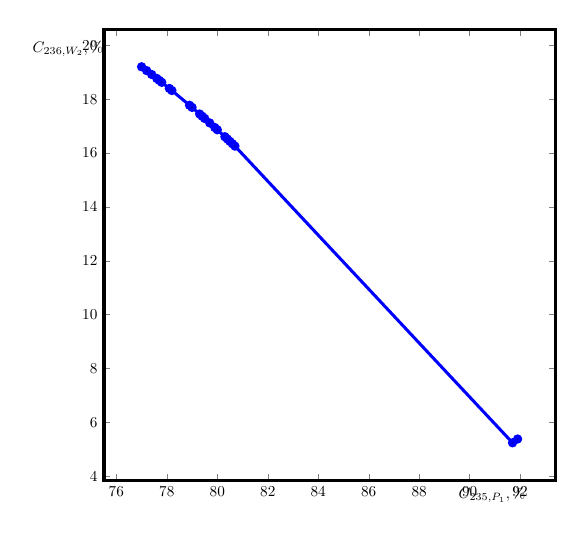
\begin{tikzpicture}[,
scale=0.55]
\begin{axis}[
  xlabel style = {{at={(axis description cs:.86,0)}}},
  ylabel = {$C_{236,W_2}, \%$},
  ylabel style = {{at={(axis description cs:-0.08,.925)},rotate=270,anchor=south}},
  xlabel = {$C_{235,P_1}, \%$},
  width=12cm, height=12cm, line width=2pt
]

\addplot+ coordinates {
  (77.0, 19.20354995742973)
  (77.2, 19.062157204472125)
  (77.4, 18.918608578311712)
  (77.60000000000001, 18.77292307609964)
  (77.7, 18.69928324668024)
  (77.8, 18.62511484136794)
  (78.10000000000001, 18.39945499658532)
  (78.2, 18.323189450313432)
  (78.9, 17.7750211540419)
  (79.0, 17.69470419345584)
  (79.3, 17.450804234311285)
  (79.4, 17.368538182322084)
  (79.5, 17.28579302654852)
  (79.7, 17.118891391179204)
  (79.9, 16.95013137456677)
  (80.0, 16.865062761747023)
  (80.30000000000001, 16.607172887205294)
  (80.4, 16.52032848882317)
  (80.5, 16.433051693388173)
  (80.60000000000001, 16.345346694722917)
  (80.7, 16.257219150399703)
  (91.7, 5.237747790489424)
  (91.9, 5.378427324120691)
};

\end{axis}
\end{tikzpicture}


% \caption{{Зависимость  концентрации $^{236}$U в потоке тяжелой фракции второго каскада $W_2$ от концентрации $^{235}$U в потоке легкой фракции первого каскада{\label{SW_l}}}}
%     \end{minipage}%
%     \begin{minipage}{.5\textwidth}
%       \centering
%       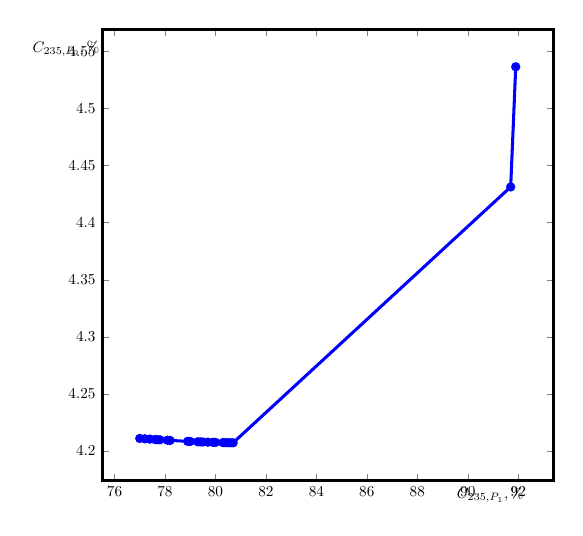
\begin{tikzpicture}[,
scale=0.55]
\begin{axis}[
  xlabel style = {{at={(axis description cs:.86,0)}}},
  ylabel = {$C_{235,P_0}, \%$},
  ylabel style = {{at={(axis description cs:-0.08,.925)},rotate=270,anchor=south}},
  xlabel = {$C_{235,P_1}, \%$},
  width=12cm, height=12cm, line width=2pt
]

\addplot+ coordinates {
  (77.0, 4.21096972553198)
  (77.2, 4.210659839435366)
  (77.4, 4.210358740398204)
  (77.60000000000001, 4.21006690040276)
  (77.7, 4.209924833527194)
  (77.8, 4.2097849356492505)
  (78.10000000000001, 4.209381303630404)
  (78.2, 4.209252109719451)
  (78.9, 4.208432990894553)
  (79.0, 4.208328602741027)
  (79.3, 4.208037634529696)
  (79.4, 4.207947919570074)
  (79.5, 4.207862044083126)
  (79.7, 4.207702088087786)
  (79.9, 4.207558613523564)
  (80.0, 4.207493381041667)
  (80.30000000000001, 4.207324521438157)
  (80.4, 4.207277603916635)
  (80.5, 4.2072354018766385)
  (80.60000000000001, 4.207198471785372)
  (80.7, 4.207166582032032)
  (91.7, 4.431200154395044)
  (91.9, 4.53639624850586)
};

\end{axis}
\end{tikzpicture}


% \caption{{Зависимость концентрации $^{235}$U в НОУ-разбавителе от концентрации $^{235}$U в потоке легкой фракции первого каскада{\label{Fnu}}}}
% \end{minipage}
% \end{figure}


\include{semestr_report/conclusion}      % Заключение
\chapter*{Список сокращений и условных обозначений} % Заголовок
\addcontentsline{toc}{chapter}{Список сокращений и условных обозначений}  % Добавляем его в оглавление
\noindent
%\begin{longtabu} to \dimexpr \textwidth-5\tabcolsep {r X}
\begin{longtabu} to \textwidth {r X}
% Жирное начертание для математических символов может иметь
% дополнительный смысл, поэтому они приводятся как в тексте
% диссертации

\(q_0\) & коэффициент разделения\\
\(N\) & длина каскада (число ступеней)\\

\(\begin{rcases}
f\\
N+1-f
\end{rcases}\)  &
число ступеней в обеднительной и обогатительной частях.
\\

\(\begin{rcases}
    n\\
    k
    \end{rcases}\)  &
    индексы целевого ($^{235}$U) и опорного компонент.
\\

\(\begin{rcases}
    F_i\\
    P_i\\
    W_i
    \end{rcases}\)  &
    потоки питания, отбора и отвала, где \textit{i} -- индекс каскада.
\\



\textbf{ЛВР} & легководный реактор \\
\textbf{ВВЭР} & водо-водяной энергетический реактор \\
\textbf{PWR} & водо-водяной энергетический реактор западного дизайна (Pressurized water reactor)\\
\textbf{ЯТЦ} & ядерный топливный цикл \\
\textbf{ЗЯТЦ} & замкнутый ядерный топливный цикл \\
\textbf{ТВС} & тепловыделяющая сборка \\
\textbf{ОТВС} & облученная тепловыделяющая сборка \\
\textbf{MOX-топливо} & ядерное топливо, состоящее из смеси диоксидов урана и плутония \\
\textbf{ОЯТ} & Облученное ядерное топливо, извлеченное из ядерного реактора после использования и для этой цели в имеющейся форме более непригодноe \\

\textbf{РАО} & Радиоактивные отходы. Существуют подклассы радиоактивных отходов: высокоактивные (ВАО), среднеактивные (САО), низкоактивные (НАО) \\




\textbf{НОУ} & низкообогащенный уран \\
\textbf{ВОУ} & высокообогащенный уран\\
%\textbf{RepU} & регенерированный уран \\
\textbf{ОГФУ} & обедненный гексафторид урана\\

\textbf{РР} & работа разделения\\
\textbf{ЕРР} & 1 кг работы разделения, единица работы по разделению изотопов. Мера усилий, затрачиваемых на разделение материала определённого изотопного состава на две фракции с отличными изотопными составами; не зависит от применяемого процесса разделения. \\

\textbf{$UF_6$} & гексафторид урана\\
\textbf{$C_{8}H_{3}F_{13}$} & фреон-346\\

\textbf{ASTM} & международное общество по испытаниям и материалам\\


\textbf{СНАУ} & система нелинейных алгебраических уравнений \\

%\textbf{Toxic Waste} & смесь с высоким содержанием минорных изотопов, классифицируемая как токсичный отход, требующий дорогостоящего хранения\\
%\textbf{mix} & смешение изотопных композиций\\


\end{longtabu}

Критерии эффективности каскадной схемы:
\begin{itemize}
    \item $(Y_f)_\text{max}$ -- максимум суммарной степени извлечения схемы (\ref{Rec2}) , соответствующий минимуму потерь $^{235}$U в схеме;
    \item $(Y_{RepU})_\text{max}$ -- максимум степени извлечения из регенерата (\ref{RecR2}), соответствующий минимуму потерь $^{235}$U регенерата;
    \item $(\delta(\frac{\Delta A}{P}))_\text{min}$ -- максимум экономии работы разделения, относительно референтной схемы трехпоточного каскада для обогащения природного урана, соответствующая минимуму удельного расхода работы разделения; 
    \item $(\delta(\frac{F_{NU}}{P}))_\text{min}$\ -- максимальная экономия природного урана относительно референтной схемы трехпоточного каскада для обогащения природного урана, соответствующая минимуму удельного расхода природного урана.
\end{itemize}\label{criteria_list}

Обозначения параметров каскадных схем:
\begin{itemize}
    \item $Y_f$ -- суммарная степень извлечения $^{235}$U в схеме \ref{Rec2};
    \item $Y_{RepU}$ -- степень извлечения $^{235}$U схемой из регенерированного урана \ref{RecR2};
    \item $\delta(\frac{\Delta A}{P})$ -- экономия работы разделения относительно референтной схемы трехпоточного каскада для обогащения природного урана. Наибольшая экономия соответствует минимуму суммарного потока схемы \ref{GrindEQ__1_73_}. Если величина отрицательная, абсолютное значение соответствует потерям работы разделения, по сравнению с референтной схемы трехпоточного каскада для обогащения природного урана.
    \item  $\frac{F_{NU}}{P}$ -- удельный расход природного урана на единицу производимого товарного НОУ;
    \item  $\delta(\frac{F_{NU}}{P})$ -- экономия природного урана относительно референтной схемы трехпоточного каскада для обогащения природного урана.  Наибольшая экономия соответствует минимуму удельного расхода природного урана схемы. Если величина отрицательная, абсолютное значение соответствует перерасходу природного урана, по сравнению с референтной схемы трехпоточного каскада для обогащения природного урана;
    \item $M_{k1}$ -- масса изотопа, выбранного в качестве опорного компонента при расчете R-каскада (\ref{GrindEQ__1_75_})--(\ref{GrindEQ__1_76_}), для первого каскада в схеме, в который поступает регенерат;
    \item $M_{k2}$ -- масса изотопа, выбранного в качестве опорного компонента при расчете R-каскада (\ref{GrindEQ__1_75_})--(\ref{GrindEQ__1_76_}), для второго каскада в схеме, на питание которого поступает поток легкой фракции первого каскада;
    \item $C_{232,\text{P}},C_{234,\text{P}},C_{235,\text{P}},C_{236,\text{P}}$ -- концентрации изотопов урана в конечном НОУ-продукте $P$;
    \item $C_{232,\text{x}},C_{234,\text{x}},C_{235,\text{x}},C_{236,\text{x}}$ -- концентрации изотопов урана в потоках $x$;
    \item $F_{x}$ -- выходные потоки, выраженные в килограммах гексафторида урана ($UF_6$), получаемые в схеме при производстве 1 тонны металического урана НОУ-продукта.
  \end{itemize}
  
\addtocounter{table}{-1}% Нужно откатить на единицу счетчик номеров таблиц, так как предыдущая таблица сделана для удобства представления информации по ГОСТ
        % Список сокращений и условных обозначений


\include{semestr_report/references}      % Список литературы


%%% Настройки для приложений
\appendix
% Оформление заголовков приложений ближе к ГОСТ:
\setlength{\midchapskip}{20pt}
\renewcommand*{\afterchapternum}{\par\nobreak\vskip \midchapskip}
\renewcommand\thechapter{\Asbuk{chapter}} % Чтобы приложения русскими буквами нумеровались

\chapter*{Приложение А}             % Заголовок
\addcontentsline{toc}{chapter}{Приложение А. Референтный ординарный трехпоточный каскад.}  % Добавляем его в оглавление
\noindent

% \counterwithin{figure}{chapter}
% \counterwithin{table}{chapter}
\renewcommand{\thefigure}{A\arabic{figure}}
\setcounter{figure}{0}
\renewcommand{\thetable}{A\arabic{table}}
\setcounter{table}{0}

\textbf{Референтный ординарный трехпоточный каскад.}

\begin{figure}[ht]
  \centerfloat{\includegraphics[scale=0.3]{cascades/ordinary/uranfN}}
  \caption{Схема ординарного каскада для обогащения природного урана}\label{uranfN}
\end{figure}

Параметры ординарного каскада для обогащения природного урана (рис. \ref{uranfN}) до 4,95\% с 0,1\% в отвале при $q_0$=1,0626586.

\begin{table}[ht]
    \centering
    \caption{Параметры схемы ординарного каскада}\label{ordninary495}
    \normalsize\begin{tabulary}{1.0\textwidth}{|c|c|c|c|c|c|}
        \hline $\frac{F}{P}$ & $\frac{P}{F}$ & $\frac{W}{F}$ & $f$ & $N$ & $\frac{\Delta A}{P}, EPP$\\
        \hline $7,93$ & $0,126$ & $0,874$ & 21,59 & 42,35 & 11,82\\\hline
    \end{tabulary}
\end{table}

\chapter*{Приложение Б}             % Заголовок
\addcontentsline{toc}{chapter}{Приложение Б. Оценка эффективности модифицированного двойного каскада по различным критериям. Дополнительные результаты.}  % Добавляем его в оглавление
\noindent

% \counterwithin{figure}{chapter}
% \counterwithin{table}{chapter}
\renewcommand{\thefigure}{Б\arabic{figure}}
\setcounter{figure}{0}
\renewcommand{\thetable}{Б\arabic{table}}
\setcounter{table}{0}

\textbf{Оценка эффективности модифицированного двойного каскада по различным критериям. Дополнительные результаты: состав 2}\label{dop2_2}

\begin{table}[ht]
  \centering
  \caption{Интегральные параметры модифицированного двойного каскада, оптимизированного по различных критериям эффективности при обогащении регенерата состава 2. Сокращения: П -- параметр; К -- критерий.{\label{2opt2_int}}}
  \begin{tabular}{|r|r||c|c|c|c|}
      \Xhline{2\arrayrulewidth}
          \diagbox{П}{К} & $({C_{235,{P_2}}})_{lim}, \%$
          & $(Y_f)_\text{max}$ & $(Y_{E})_\text{max}$ & $(\delta(\frac{\Delta A}{P}))_\text{min}$ & $(\delta(\frac{F_{NU}}{P}))_\text{min}$ \\ \Xhline{2\arrayrulewidth}
      \multirow{2}{*}{$Y_f, \%$}
          & 20 & 85.51 & 85.51 & 75.5 & 85.49 \\\cline{2-6} 
          & 90 & 88.21 & 88.21 & 75.5 & 87.27 \\
      \Xhline{2\arrayrulewidth}
      \multirow{2}{*}{$Y_{E}, \%$}
          & 20 &  74.53 & 74.53 & 6.83 & 74.46 \\\cline{2-6} 
          & 90 &  90.88 & 90.88 & 6.81 & 83.6 \\
      \Xhline{2\arrayrulewidth}
      \multirow{2}{*}{$\delta(\frac{\Delta A}{P}), \%$}
          & 20 & -5.311 & -5.311 & 0.487 & -8.702 \\\cline{2-6} 
          & 90 & -5.571 & -5.571 & 0.509 & -14.15 \\
      \Xhline{2\arrayrulewidth}
      \multirow{2}{*}{$\delta(\frac{F_{NU}}{P}), \%$}
          & 20 & 9.925 & 9.925 & 0.9767 & 10.62 \\\cline{2-6} 
          & 90 & 13.22 & 13.22 & 0.9801 & 16.11\\
\Xhline{2\arrayrulewidth}
      \end{tabular}
\end{table}

\begin{table}[ht]
  \centering
  \caption{Параметры модифицированного двойного каскада, оптимизированного по различных критериям эффективности при обогащении регенерата состава 2. Сокращения: П -- параметр; К -- критерий.{\label{2opt2}}}
  \begin{tabular}{|r|r||c|c|c|c|}
      \Xhline{2\arrayrulewidth}
          \diagbox{П}{К} & $({C_{235,{P_2}}})_{lim}, \%$
          & $(Y_f)_\text{max}$ & $(Y_{E})_\text{max}$ & $(\delta(\frac{\Delta A}{P}))_\text{min}$ & $(\delta(\frac{F_{NU}}{P}))_\text{min}$ \\ \Xhline{2\arrayrulewidth}
      \multirow{2}{*}{$C_{232,P}, \%$}
          & 20 & $5,0\cdot10^{-7}$ & $5,0\cdot10^{-7}$ & $1,424\cdot10^{-7}$ & $5,0\cdot10^{-7}$ \\\cline{2-6} 
          & 90 & $5,0\cdot10^{-7}$ & $5,0\cdot10^{-7}$  & $1,369\cdot10^{-7}$ & $5,0\cdot10^{-7}$  \\\Xhline{2\arrayrulewidth}
      \multirow{2}{*}{$C_{235,P}, \%$}
          & 20 &  5,10 & 5,137 & 5,147 & 5,025 \\\cline{2-6} 
          & 90 &  5,195 & 5,195 & 4,969 & 5,161 \\
      \Xhline{2\arrayrulewidth}
      \multirow{2}{*}{$C_{236,P}, \%$}
          & 20 & 0,5165 & 0,6444 & 0,68 & 0,2597 \\\cline{2-6} 
          & 90 & 0,8463 & 0,8463 & 0,06389 & 0,7265 \\
      \Xhline{2\arrayrulewidth}
      \multirow{2}{*}{$M_{k1}, M_{k2}$}
          & 20 & 6  6 & 6  6 & 8  6 & 6  2 \\\cline{2-6} 
          & 90 & 8   2 & 8   2 & 4   2 & 6   2\\
      \Xhline{2\arrayrulewidth}
      \multirow{2}{*}{$C_{232,P_{1}}, \%$}
          & 20 & $6,80\cdot10^{-6}$ & $6,80\cdot10^{-6}$ & $8,17\cdot10^{-6}$ & $6,74\cdot10^{-6}$ \\\cline{2-6} 
          & 90 & $6,19\cdot10^{-5}$ & $6,19\cdot10^{-5}$ & $8,55\cdot10^{-6}$ & $8,60\cdot10^{-5}$\\
      \Xhline{2\arrayrulewidth}
      \multirow{2}{*}{$C_{232,P_{2}}, \%$}
          & 20 & $5,15\cdot10^{-5}$ & $5,15\cdot10^{-5}$ & $1,83\cdot10^{-4}$ & $5,13\cdot10^{-5}$ \\\cline{2-6}
          & 90 & $2,57\cdot10^{-3}$ & $2,57\cdot10^{-3}$ & $2,67\cdot10^{-3}$ & $5,548\cdot10^{-4}$\\
      \Xhline{2\arrayrulewidth}
      \multirow{2}{*}{$C_{235,P_{1}}, \%$}
          & 20 & 6,516 & 6,516 & 3,554 & 6,456 \\\cline{2-6} 
          & 90 & 5,943 & 5,943 & 3,657 & 81,19\\
      \Xhline{2\arrayrulewidth}
      \multirow{2}{*}{$C_{235,W_{2}}, \%$}
          & 20 & 5,629 & 5,629 & 3,472 & 5,569 \\\cline{2-6} 
          & 90 & 5,866 & 5,866 & 3,625 & 80,75\\
  \Xhline{2\arrayrulewidth}
      \multirow{2}{*}{$C_{235,P_{2}}, \%$}
          & 20 & 19,76 & 19,76 & 19,76 & 19,76 \\\cline{2-6} 
          & 90 & 73,3 & 73,3 & 73,76 & 86,65\\
      \Xhline{2\arrayrulewidth}
      \multirow{2}{*}{$C_{235,P_{n}}, \%$}
          & 20 & 5,13 & 5,13 & 4,998 & 5,098 \\\cline{2-6} 
          & 90 & 5,074 & 5,074 & 4,994 & 4,211\\
      \Xhline{2\arrayrulewidth}           
      \multirow{2}{*}{$P_2$, кг}
        & 20 & 13,01 & 13,01 & 0,1463 & 13,08 \\\cline{2-6} 
        & 90 & 0,2607 & 0,2607 & 0,01245 & 1,21\\
\Xhline{2\arrayrulewidth}
      \end{tabular}
\end{table}


\newpage

\chapter*{Приложение В}             % Заголовок
\addcontentsline{toc}{chapter}{Приложение В. Анализ <<устойчивости>> схемы двойного каскада с НОУ-разбавителем к изменению внешних условий. Дополнительные результаты.}  % Добавляем его в оглавление
\noindent

% \counterwithin{figure}{chapter}
% \counterwithin{table}{chapter}
\renewcommand{\thefigure}{В\arabic{figure}}
\setcounter{figure}{0}
\renewcommand{\thetable}{В\arabic{table}}
\setcounter{table}{0}

\textbf{Анализ <<устойчивости>> схемы двойного каскада с НОУ-разбавителем к изменению внешних условий. Дополнительные результаты.}

\begin{figure}
    \centering
    \begin{minipage}{.5\textwidth}
      \centering
      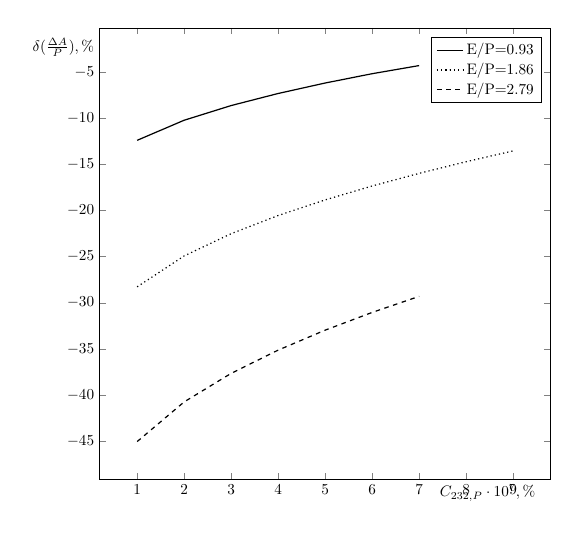
\begin{tikzpicture}[,
scale=0.55]
\begin{axis}[
  xlabel style = {{at={(axis description cs:.86,0)}}},
  ylabel = {$\delta(\frac{\Delta A}{P}), \%$},
  ylabel style = {{at={(axis description cs:-0.08,.925)},rotate=270,anchor=south}},
  xlabel = {$C_{232,P}\cdot10^{7}, \%$},
  width=12cm, height=12cm
]

\addplot+[mark=none,
  solid, black, thick
] coordinates {
  (1.0, -12.395218440946906)
  (2.0, -10.219020529323354)
  (3.0000000000000004, -8.626929870001328)
  (4.0, -7.3185844692402915)
  (5.0, -6.185264012646069)
  (6.0, -5.173768588868835)
  (7.000000000000001, -4.29293979177781)
};
\addlegendentry{{}{E/P=0.93}}

\addplot+[mark=none,
  dotted, black, thick
] coordinates {
  (1.0, -28.282242175940937)
  (2.0, -24.929077234925025)
  (3.0000000000000004, -22.516662376271356)
  (4.0, -20.550634890717415)
  (5.0, -18.85615249546271)
  (6.0, -17.34800036201673)
  (7.000000000000001, -15.978805541243855)
  (8.0, -14.71681616393461)
  (9.000000000000002, -13.541592549068923)
};
\addlegendentry{{}{E/P=1.86}}

\addplot+[mark=none,
  dashed, black, thick
] coordinates {
  (1.0, -45.057945429681226)
  (2.0, -40.758242565718376)
  (3.0000000000000004, -37.66157309459905)
  (4.0, -35.14302713983917)
  (5.0, -32.97793340752656)
  (6.0, -31.056144200883885)
  (7.000000000000001, -29.31422868906391)
};
\addlegendentry{{}{E/P=2.79}}

\end{axis}
\end{tikzpicture}


      \caption{{Зависимость экономии работы разделения от ПДК $^{232}$U в НОУ-продукте с обогащением до уровня 4,4\% для различных $\frac{E}{P}$.{\label{sw44}}}}
    \end{minipage}%
    \begin{minipage}{.5\textwidth}
      \centering
      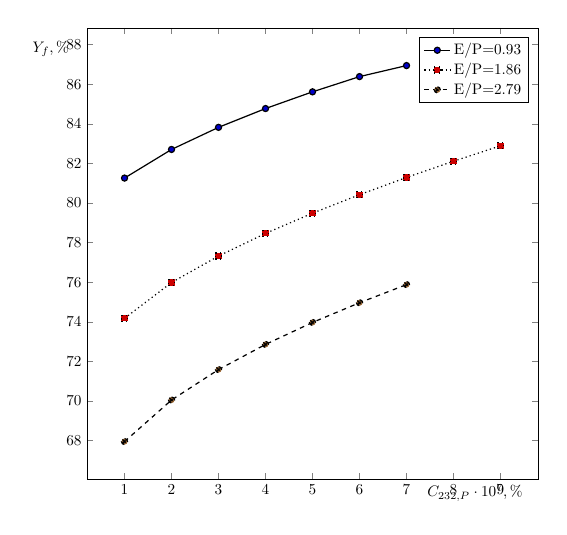
\begin{tikzpicture}[,
scale=0.55]
\begin{axis}[
  xlabel style = {{at={(axis description cs:.86,0)}}},
  ylabel = {$Y_{f}, \%$},
  ylabel style = {{at={(axis description cs:-0.08,.925)},rotate=270,anchor=south}},
  xlabel = {$C_{232,P}\cdot10^{7}, \%$},
  width=12cm, height=12cm
]

\addplot+[
  solid, black, thick
] coordinates {
  (1.0, 81.2599146274243)
  (2.0, 82.70510635581616)
  (3.0000000000000004, 83.82183689954859)
  (4.0, 84.77127401369083)
  (5.0, 85.61487919146296)
  (6.0, 86.38356067088392)
  (7.000000000000001, 86.94074198596759)
};
\addlegendentry{{}{E/P=0.93}}

\addplot+[
  dotted, black, thick
] coordinates {
  (1.0, 74.17655829999579)
  (2.0, 75.98498213201852)
  (3.0000000000000004, 77.32265969408223)
  (4.0, 78.46540402752339)
  (5.0, 79.48580928842689)
  (6.0, 80.42063662698051)
  (7.000000000000001, 81.29053109508794)
  (8.0, 82.1100269832236)
  (9.000000000000002, 82.88835691546974)
};
\addlegendentry{{}{E/P=1.86}}

\addplot+[
  dashed, black, thick
] coordinates {
  (1.0, 67.95360281561639)
  (2.0, 70.05234164130057)
  (3.0000000000000004, 71.58870177419513)
  (4.0, 72.85958391192455)
  (5.0, 73.97031718490105)
  (6.0, 74.96387446964957)
  (7.000000000000001, 75.87957963032518)
};
\addlegendentry{{}{E/P=2.79}}

\end{axis}
\end{tikzpicture}


      \caption{{Зависимость степени извлечения $^{235}$U из регенерата от ПДК $^{232}$U в НОУ-продукте с обогащением до уровня 4,4\% для различных $\frac{E}{P}$.{\label{exR44}}}}
    \end{minipage}
\end{figure}

\begin{figure}
    \centering
    \begin{minipage}{.5\textwidth}
      \centering
      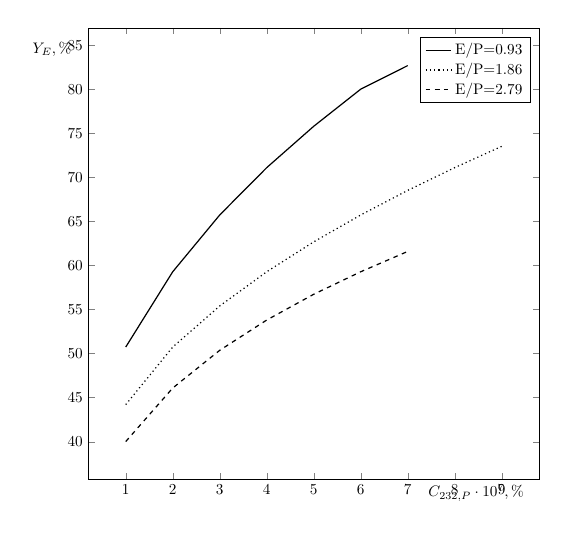
\begin{tikzpicture}[,
scale=0.55]
\begin{axis}[
  xlabel style = {{at={(axis description cs:.86,0)}}},
  ylabel = {$Y_{E}, \%$},
  ylabel style = {{at={(axis description cs:-0.08,.925)},rotate=270,anchor=south}},
  xlabel = {$C_{232,P}\cdot10^{7}, \%$},
  width=12cm, height=12cm
]

\addplot+[mark=none,
  solid, black, thick
] coordinates {
  (1.0, 50.745320366220234)
  (2.0, 59.30149726322195)
  (3.0000000000000004, 65.7519664106782)
  (4.0, 71.12954522207235)
  (5.0, 75.82763880377072)
  (6.0, 80.04430359281832)
  (7.000000000000001, 82.72459665893969)
};
\addlegendentry{{}{E/P=0.93}}

\addplot+[mark=none,
  dotted, black, thick
] coordinates {
  (1.0, 44.20353110984807)
  (2.0, 50.745320366220234)
  (3.0000000000000004, 55.41327633341921)
  (4.0, 59.30149726322195)
  (5.0, 62.69903149138577)
  (6.0, 65.75196641067834)
  (7.000000000000001, 68.5430309981216)
  (8.0, 71.12954522207235)
  (9.000000000000002, 73.54852477832327)
};
\addlegendentry{{}{E/P=1.86}}

\addplot+[mark=none,
  dashed, black, thick
] coordinates {
  (1.0, 40.009414250517715)
  (2.0, 46.09394772079198)
  (3.0000000000000004, 50.37816062607195)
  (4.0, 53.81590263606467)
  (5.0, 56.74369030977263)
  (6.0, 59.30149726322191)
  (7.000000000000001, 61.61037730716592)
};
\addlegendentry{{}{E/P=2.79}}

\end{axis}
\end{tikzpicture}


\caption{{Зависимость степени извлечения $^{235}$U из регенерата от ПДК $^{232}$U в НОУ-продукте с обогащением до уровня 4,4\% для различных $\frac{E}{P}$.{\label{exR44}}}}
    \end{minipage}%
    \begin{minipage}{.5\textwidth}
      \centering
      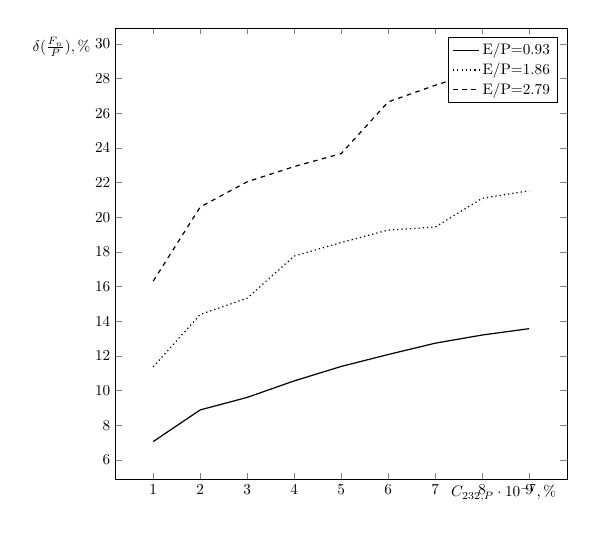
\begin{tikzpicture}[,
scale=0.55]
\begin{axis}[
  xlabel style = {{at={(axis description cs:.86,0)}}},
  ylabel = {$\delta(\frac{F_n}{P}), \%$},
  ylabel style = {{at={(axis description cs:-0.12,.925)},rotate=270,anchor=south}},
  xlabel = {$C_{232,P}\cdot10^{-7}, \%$},
  width=12cm, height=12cm
]

\addplot+[mark=none,
  solid, black, thick
] coordinates {
  (1.0, 7.057760090703368)
  (2.0, 8.883437157947327)
  (3.0000000000000004, 9.605444995054558)
  (4.0, 10.55710068193495)
  (5.0, 11.39016688359421)
  (6.0, 12.079179244566795)
  (7.000000000000001, 12.731349141503689)
  (8.0, 13.2030657848923)
  (9.000000000000002, 13.570378177156261)
};
\addlegendentry{{}{E/P=0.93}}

\addplot+[mark=none,
  dotted, black, thick
] coordinates {
  (1.0, 11.365686755446403)
  (2.0, 14.388303949542236)
  (3.0000000000000004, 15.32915753801609)
  (4.0, 17.755819239592196)
  (5.0, 18.538942955684167)
  (6.0, 19.25590180171489)
  (7.000000000000001, 19.428633887556103)
  (8.0, 21.089075670500623)
  (9.000000000000002, 21.52560986675717)
};
\addlegendentry{{}{E/P=1.86}}

\addplot+[mark=none,
  dashed, black, thick
] coordinates {
  (1.0, 16.31337535716355)
  (2.0, 20.58636758324206)
  (3.0000000000000004, 22.044054253914446)
  (4.0, 22.920132708437947)
  (5.0, 23.667999814578412)
  (6.0, 26.65031148325815)
  (7.000000000000001, 27.607494173667078)
  (8.0, 28.461707300289373)
  (9.000000000000002, 28.74364899102281)
};
\addlegendentry{{}{E/P=2.79}}

\end{axis}
\end{tikzpicture}

\caption{{Зависимость расхода природного урана от ПДК $^{232}$U в НОУ-продукте с обогащением до уровня 4,4\% для различных $\frac{E}{P}$.{\label{F0R44}}}}
    \end{minipage}
\end{figure}

\begin{figure}
    \centering
    \begin{minipage}{.5\textwidth}
      \centering
      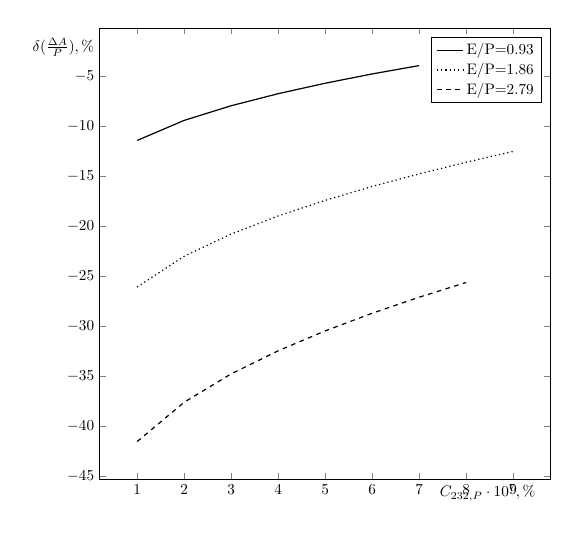
\begin{tikzpicture}[,
scale=0.55]
\begin{axis}[
  xlabel style = {{at={(axis description cs:.86,0)}}},
  ylabel = {$\delta(\frac{\Delta A}{P}), \%$},
  ylabel style = {{at={(axis description cs:-0.08,.925)},rotate=270,anchor=south}},
  xlabel = {$C_{232,P}\cdot10^{7}, \%$},
  width=12cm, height=12cm
]

\addplot+[mark=none,
  solid, black, thick
] coordinates {
  (1.0, -11.442050325962452)
  (2.0, -9.438723200431037)
  (3.0000000000000004, -7.9728246964313)
  (4.0, -6.768022196914314)
  (5.0, -5.7242794711367315)
  (6.0, -4.7922989130984135)
  (7.000000000000001, -3.956523255555432)
};
\addlegendentry{{}{E/P=0.93}}

\addplot+[mark=none,
  dotted, black, thick
] coordinates {
  (1.0, -26.09957395082424)
  (2.0, -23.022672963318332)
  (3.0000000000000004, -20.802863046158134)
  (4.0, -18.993519736891432)
  (5.0, -17.43387788617293)
  (6.0, -16.045572170953353)
  (7.000000000000001, -14.785062105867015)
  (8.0, -13.623128278493162)
  (9.000000000000002, -12.541001761914492)
};
\addlegendentry{{}{E/P=1.86}}

\addplot+[mark=none,
  dashed, black, thick
] coordinates {
  (1.0, -41.554133458995025)
  (2.0, -37.62214258113987)
  (3.0000000000000004, -34.78539667116384)
  (4.0, -32.475395453374304)
  (5.0, -30.487594682338603)
  (6.0, -28.721514147914533)
  (7.000000000000001, -27.11944341607787)
  (8.0, -25.644440494125277)
};
\addlegendentry{{}{E/P=2.79}}

\end{axis}
\end{tikzpicture}


\caption{{Зависимость экономии работы разделения от ПДК $^{232}$U в НОУ-продукте с обогащением до уровня 4,7\% для различных $\frac{E}{P}$.{\label{sw47}}}}
    \end{minipage}%
    \begin{minipage}{.5\textwidth}
      \centering
      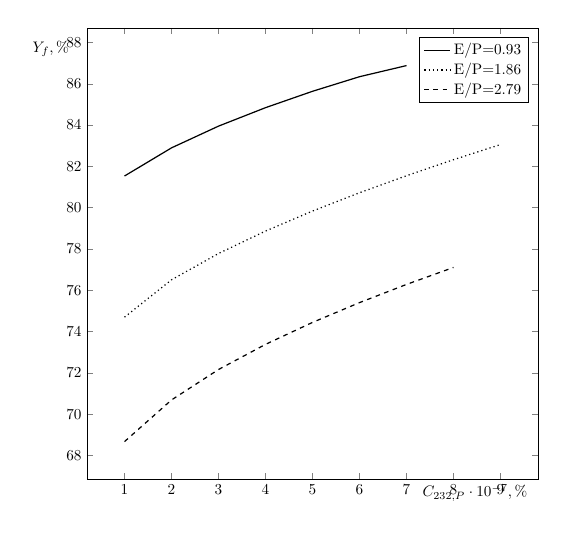
\begin{tikzpicture}[,
scale=0.55]
\begin{axis}[
  xlabel style = {{at={(axis description cs:.86,0)}}},
  ylabel = {$Y_{f}, \%$},
  ylabel style = {{at={(axis description cs:-0.08,.925)},rotate=270,anchor=south}},
  xlabel = {$C_{232,P}\cdot10^{-7}, \%$},
  width=12cm, height=12cm
]

\addplot+[mark=none,
  solid, black, thick
] coordinates {
  (1.0, 81.53156037359754)
  (2.0, 82.89545086273719)
  (3.0000000000000004, 83.9478345607235)
  (4.0, 84.84152401044177)
  (5.0, 85.63479347902604)
  (6.0, 86.3412156692256)
  (7.000000000000001, 86.88027992336104)
};
\addlegendentry{{}{E/P=0.93}}

\addplot+[mark=none,
  dotted, black, thick
] coordinates {
  (1.0, 74.69415676339759)
  (2.0, 76.50476826786495)
  (3.0000000000000004, 77.77849512744808)
  (4.0, 78.86515635925242)
  (5.0, 79.83436020530084)
  (6.0, 80.72135365193532)
  (7.000000000000001, 81.54594313296484)
  (8.0, 82.32205886834831)
  (9.000000000000002, 83.05589060957709)
};
\addlegendentry{{}{E/P=1.86}}

\addplot+[mark=none,
  dashed, black, thick
] coordinates {
  (1.0, 68.6697629941284)
  (2.0, 70.68575248489067)
  (3.0000000000000004, 72.15973261088106)
  (4.0, 73.37774759491083)
  (5.0, 74.44135268684659)
  (6.0, 75.39965734146578)
  (7.000000000000001, 76.28121651908731)
  (8.0, 77.10358771087932)
};
\addlegendentry{{}{E/P=2.79}}

\end{axis}
\end{tikzpicture}


\caption{{Зависимость степени извлечения $^{235}$U от ПДК $^{232}$U в НОУ-продукте с обогащением до уровня 4,7\% для различных $\frac{E}{P}$.{\label{ex47}}}}
\end{minipage}
\end{figure}

\begin{figure}
    \centering
    \begin{minipage}{.5\textwidth}
      \centering
      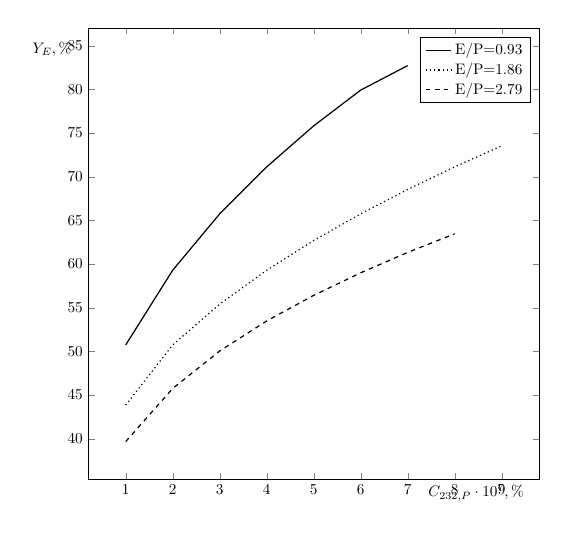
\begin{tikzpicture}[,
scale=0.55]
\begin{axis}[
  xlabel style = {{at={(axis description cs:.86,0)}}},
  ylabel = {$Y_{E}, \%$},
  ylabel style = {{at={(axis description cs:-0.08,.925)},rotate=270,anchor=south}},
  xlabel = {$C_{232,P}\cdot10^{7}, \%$},
  width=12cm, height=12cm
]

\addplot+[mark=none,
  solid, black, thick
] coordinates {
  (1.0, 50.74532036622023)
  (2.0, 59.30149726322195)
  (3.0000000000000004, 65.75196641067834)
  (4.0, 71.12954522207235)
  (5.0, 75.82763880377072)
  (6.0, 79.9222355420343)
  (7.000000000000001, 82.72736369212772)
};
\addlegendentry{{}{E/P=0.93}}

\addplot+[mark=none,
  dotted, black, thick
] coordinates {
  (1.0, 43.8508093556669)
  (2.0, 50.745320366220234)
  (3.0000000000000004, 55.41327633341921)
  (4.0, 59.30149726322195)
  (5.0, 62.699031491385725)
  (6.0, 65.75196641067818)
  (7.000000000000001, 68.5430309981216)
  (8.0, 71.12954522207235)
  (9.000000000000002, 73.53797277442622)
};
\addlegendentry{{}{E/P=1.86}}

\addplot+[mark=none,
  dashed, black, thick
] coordinates {
  (1.0, 39.675583995839325)
  (2.0, 45.761133085161255)
  (3.0000000000000004, 50.047914553011395)
  (4.0, 53.488618646439654)
  (5.0, 56.419645475250455)
  (6.0, 59.003049808125226)
  (7.000000000000001, 61.33254693680554)
  (8.0, 63.465686451699256)
};
\addlegendentry{{}{E/P=2.79}}

\end{axis}
\end{tikzpicture}


\caption{{Зависимость степени извлечения $^{235}$U из регенерата от ПДК $^{232}$U в НОУ-продукте с обогащением до уровня 4,7\% для различных $\frac{E}{P}$.{\label{exR47}}}}
    \end{minipage}%
    \begin{minipage}{.5\textwidth}
      \centering
      \begin{tikzpicture}[,
scale=0.55]
\begin{axis}[
  xlabel style = {{at={(axis description cs:.86,0)}}},
  ylabel = {$\frac{F_{NU}}{P}, \text{кг}$},
  ylabel style = {{at={(axis description cs:-0.12,.925)},rotate=270,anchor=south}},
  xlabel = {$C_{232,P}\cdot10^{7}, \%$},
  width=12cm, height=12cm
]

\addplot+[
  solid, black, thick
] coordinates {
  (1.0, 706.6354192785525)
  (2.0, 695.5705180447756)
  (3.0000000000000004, 687.235363636582)
  (4.0, 680.2789392306238)
  (5.0, 674.1924129651806)
  (6.0, 668.7266457264177)
  (7.000000000000001, 663.5511601107812)
};
\addlegendentry{{}{E/P=0.93}}

\addplot+[
  dotted, black, thick
] coordinates {
  (1.0, 677.959887355208)
  (2.0, 661.022268767328)
  (3.0000000000000004, 648.9416341028616)
  (4.0, 638.8924683215785)
  (5.0, 630.1132051976982)
  (6.0, 622.2220219123312)
  (7.000000000000001, 615.0034218929161)
  (8.0, 608.3093364348874)
  (9.000000000000002, 602.0503886358283)
};
\addlegendentry{{}{E/P=1.86}}

\addplot+[
  dashed, black, thick
] coordinates {
  (1.0, 654.2885822321769)
  (2.0, 632.4090216922981)
  (3.0000000000000004, 616.5981030031621)
  (4.0, 603.7017776368674)
  (5.0, 592.5838268649425)
  (6.0, 582.6875967531196)
  (7.000000000000001, 573.6906309431884)
  (8.0, 565.3894655334504)
};
\addlegendentry{{}{E/P=2.79}}

\end{axis}
\end{tikzpicture}


\caption{{Зависимость расхода природного урана от ПДК $^{232}$U в НОУ-продукте с обогащением до уровня 4,7\% для различных $\frac{E}{P}$.{\label{F0R47}}}}
\end{minipage}
\end{figure}

\begin{figure}
    \centering
    \begin{minipage}{.5\textwidth}
      \centering
      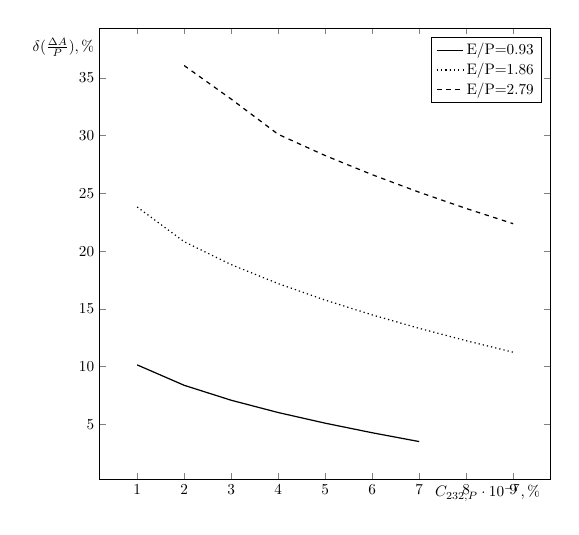
\begin{tikzpicture}[,
scale=0.55]
\begin{axis}[
  xlabel style = {{at={(axis description cs:.86,0)}}},
  ylabel = {$\delta(\frac{\Delta A}{P}), \%$},
  ylabel style = {{at={(axis description cs:-0.08,.925)},rotate=270,anchor=south}},
  xlabel = {$C_{232,P}\cdot10^{-7}, \%$},
  width=12cm, height=12cm
]

\addplot+[mark=none,
  solid, black, thick
] coordinates {
  (1.0, 10.149838341711135)
  (2.0, 8.382155711990722)
  (3.0000000000000004, 7.088371632908093)
  (4.0, 6.0248508842357245)
  (5.0, 5.102882323296978)
  (6.0, 4.273113201042603)
  (7.000000000000001, 3.509602428442813)
};
\addlegendentry{{}{E/P=0.93}}

\addplot+[mark=none,
  dotted, black, thick
] coordinates {
  (1.0, 23.823133024898677)
  (2.0, 20.815838403670245)
  (3.0000000000000004, 18.832982700086603)
  (4.0, 17.18881625250314)
  (5.0, 15.758547005316414)
  (6.0, 14.479894930684239)
  (7.000000000000001, 13.316185752259024)
  (8.0, 12.243723663525396)
  (9.000000000000002, 11.246222146183511)
};
\addlegendentry{{}{E/P=1.86}}

\addplot+[mark=none,
  dashed, black, thick
] coordinates {
  (2.0, 36.066525267783106)
  (3.0000000000000004, 33.16682579758896)
  (4.0, 30.115313378877072)
  (5.0, 28.275805724474395)
  (6.0, 26.618567158713446)
  (7.000000000000001, 25.10030828410702)
  (8.0, 23.692935156588334)
  (9.000000000000002, 22.376908192213214)
};
\addlegendentry{{}{E/P=2.79}}

\end{axis}
\end{tikzpicture}


      \caption{{Зависимость экономии работы разделения от ПДК $^{232}$U в НОУ-продукте с обогащением до уровня 5,2\% для различных $\frac{E}{P}$.{\label{sw52}}}}
    \end{minipage}%
    \begin{minipage}{.5\textwidth}
      \centering
      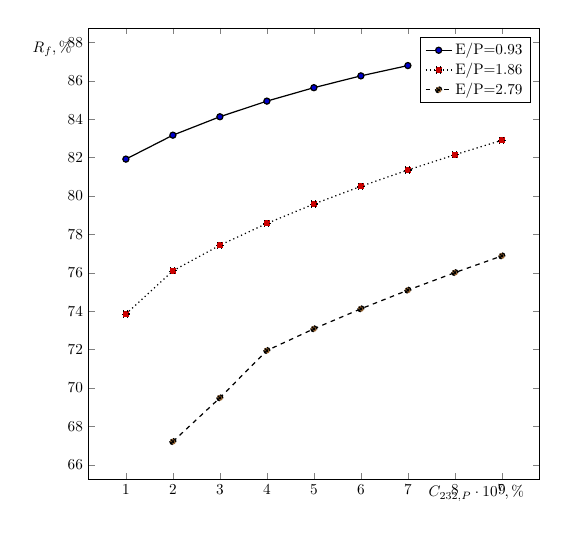
\begin{tikzpicture}[,
scale=0.55]
\begin{axis}[
  xlabel style = {{at={(axis description cs:.86,0)}}},
  ylabel = {$R_{f}, \%$},
  ylabel style = {{at={(axis description cs:-0.08,.925)},rotate=270,anchor=south}},
  xlabel = {$C_{232,P}\cdot10^{7}, \%$},
  width=12cm, height=12cm
]

\addplot+[
  solid, black, thick
] coordinates {
  (1.0, 81.92047282281692)
  (2.0, 83.16742538966415)
  (3.0000000000000004, 84.12759194071681)
  (4.0, 84.94161765082885)
  (5.0, 85.64166453585005)
  (6.0, 86.25729994352187)
  (7.000000000000001, 86.79329916754914)
};
\addlegendentry{{}{E/P=0.93}}

\addplot+[
  dotted, black, thick
] coordinates {
  (1.0, 73.84598056878988)
  (2.0, 76.10056358211024)
  (3.0000000000000004, 77.43294968555689)
  (4.0, 78.56987165120975)
  (5.0, 79.5809470624556)
  (6.0, 80.50160145898167)
  (7.000000000000001, 81.35303037639089)
  (8.0, 82.14905252951476)
  (9.000000000000002, 82.89921358322908)
};
\addlegendentry{{}{E/P=1.86}}

\addplot+[
  dashed, black, thick
] coordinates {
  (2.0, 67.20594201450372)
  (3.0000000000000004, 69.48318645671289)
  (4.0, 71.94804280408532)
  (5.0, 73.08027680473819)
  (6.0, 74.12135493795347)
  (7.000000000000001, 75.09259182720001)
  (8.0, 76.00791338569806)
  (9.000000000000002, 76.87705901175764)
};
\addlegendentry{{}{E/P=2.79}}

\end{axis}
\end{tikzpicture}


      \caption{{Зависимость степени извлечения $^{235}$U из регенерата от ПДК $^{232}$U в НОУ-продукте с обогащением до уровня 5,2\% для различных $\frac{E}{P}$.{\label{exR52}}}}
    \end{minipage}
\end{figure}

\begin{figure}
    \centering
    \begin{minipage}{.5\textwidth}
      \centering
      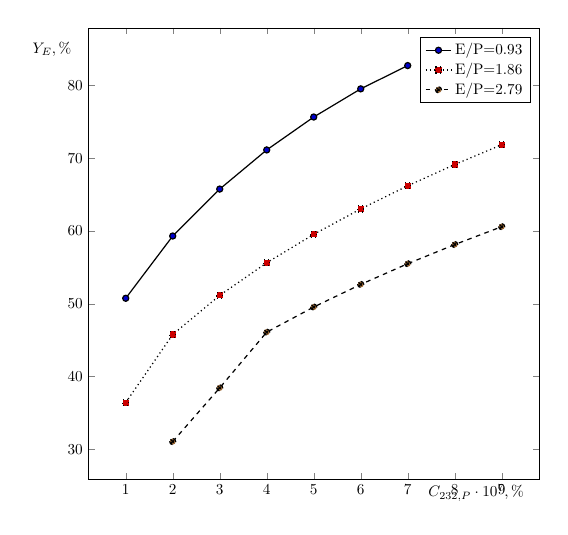
\begin{tikzpicture}[,
scale=0.55]
\begin{axis}[
  xlabel style = {{at={(axis description cs:.86,0)}}},
  ylabel = {$Y_{E}, \%$},
  ylabel style = {{at={(axis description cs:-0.08,.925)},rotate=270,anchor=south}},
  xlabel = {$C_{232,P}\cdot10^{7}, \%$},
  width=12cm, height=12cm
]

\addplot+[
  solid, black, thick
] coordinates {
  (1.0, 50.745320366220206)
  (2.0, 59.30149726322206)
  (3.0000000000000004, 65.75196641067834)
  (4.0, 71.1295452220723)
  (5.0, 75.6532981285366)
  (6.0, 79.52272196391077)
  (7.000000000000001, 82.72253492281729)
};
\addlegendentry{{}{E/P=0.93}}

\addplot+[
  dotted, black, thick
] coordinates {
  (1.0, 36.4111106586823)
  (2.0, 45.76462199063639)
  (3.0000000000000004, 51.14102895339182)
  (4.0, 55.622818080555916)
  (5.0, 59.52901295979165)
  (6.0, 63.02235936849755)
  (7.000000000000001, 66.20030038850088)
  (8.0, 69.12649182519807)
  (9.000000000000002, 71.84506168392848)
};
\addlegendentry{{}{E/P=1.86}}

\addplot+[
  dashed, black, thick
] coordinates {
  (2.0, 31.052928837106435)
  (3.0000000000000004, 38.434804849560365)
  (4.0, 46.09143609388377)
  (5.0, 49.541981912692776)
  (6.0, 52.64930445174624)
  (7.000000000000001, 55.493065127672466)
  (8.0, 58.12552740420125)
  (9.000000000000002, 60.58336009265791)
};
\addlegendentry{{}{E/P=2.79}}

\end{axis}
\end{tikzpicture}


\caption{{Зависимость степени извлечения $^{235}$U из регенерата от ПДК $^{232}$U в НОУ-продукте с обогащением до уровня 5,2\% для различных $\frac{E}{P}$.{\label{exR52}}}}
    \end{minipage}%
    \begin{minipage}{.5\textwidth}
      \centering
      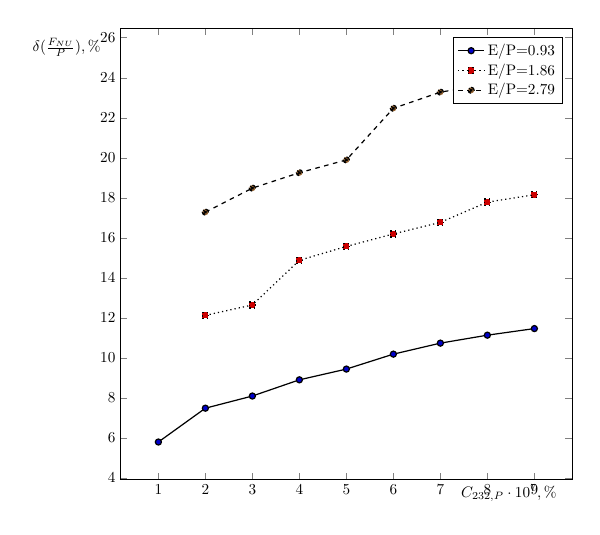
\begin{tikzpicture}[,
scale=0.55]
\begin{axis}[
  xlabel style = {{at={(axis description cs:.86,0)}}},
  ylabel = {$\delta(\frac{F_{NU}}{P}), \%$},
  ylabel style = {{at={(axis description cs:-0.12,.925)},rotate=270,anchor=south}},
  xlabel = {$C_{232,P}\cdot10^{7}, \%$},
  width=12cm, height=12cm
]

\addplot+[
  solid, black, thick
] coordinates {
  (1.0, 5.793046394428947)
  (2.0, 7.4830576011553855)
  (3.0000000000000004, 8.091358069070598)
  (4.0, 8.901084905310231)
  (5.0, 9.438059464830372)
  (6.0, 10.18430556091351)
  (7.000000000000001, 10.734274883113482)
  (8.0, 11.131996659369692)
  (9.000000000000002, 11.461858128710666)
};
\addlegendentry{{}{E/P=0.93}}

\addplot+[
  dotted, black, thick
] coordinates {
  (2.0, 12.123287852615794)
  (3.0000000000000004, 12.641245614364582)
  (4.0, 14.874069679925771)
  (5.0, 15.566658207311013)
  (6.0, 16.191082381194388)
  (7.000000000000001, 16.769702434887257)
  (8.0, 17.780984910214105)
  (9.000000000000002, 18.14904312365678)
};
\addlegendentry{{}{E/P=1.86}}

\addplot+[
  dashed, black, thick
] coordinates {
  (2.0, 17.28090551539224)
  (3.0000000000000004, 18.480641817808085)
  (4.0, 19.250290190147645)
  (5.0, 19.889420973493365)
  (6.0, 22.4698704842767)
  (7.000000000000001, 23.276906871527515)
  (8.0, 23.66795997375587)
  (9.000000000000002, 24.581976879770806)
};
\addlegendentry{{}{E/P=2.79}}

\end{axis}
\end{tikzpicture}


\caption{{Зависимость расхода природного урана от ПДК $^{232}$U в НОУ-продукте с обогащением до уровня 5,2\% для различных $\frac{E}{P}$.{\label{F0R52}}}}
    \end{minipage}
\end{figure}

\begin{figure}
    \centering
    \begin{minipage}{.5\textwidth}
      \centering
      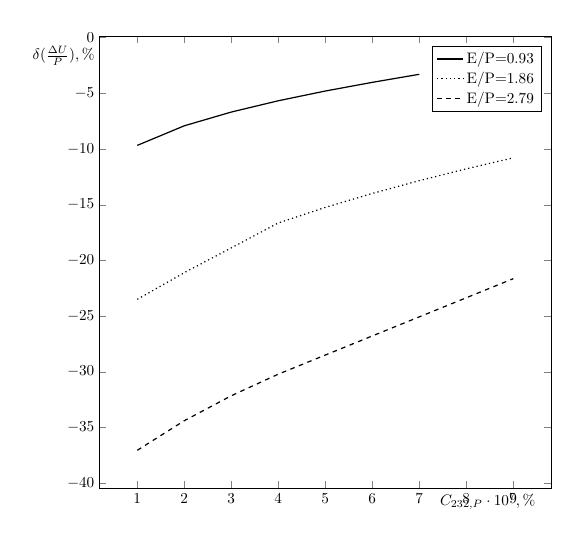
\begin{tikzpicture}[,
scale=0.55]
\begin{axis}[
  xlabel style = {{at={(axis description cs:.86,0)}}},
  ylabel = {$\delta(\frac{\Delta U}{P}), \%$},
  ylabel style = {{at={(axis description cs:-0.08,.925)},rotate=270,anchor=south}},
  xlabel = {$C_{232,P}\cdot10^{7}, \%$},
  width=12cm, height=12cm
]

\addplot+[mark=none,
  solid, black, thick
] coordinates {
  (1.0, -9.674911908891808)
  (2.0, -7.916580534549614)
  (3.0000000000000004, -6.681867721811178)
  (4.0, -5.6678082447103755)
  (5.0, -4.794275755390127)
  (6.0, -4.014408958772108)
  (7.000000000000001, -3.2916785299194777)
};
\addlegendentry{{}{E/P=0.93}}

\addplot+[mark=none,
  dotted, black, thick
] coordinates {
  (1.0, -23.50106092571201)
  (2.0, -21.106953058591188)
  (3.0000000000000004, -18.88217189205597)
  (4.0, -16.643364366696886)
  (5.0, -15.246115172124236)
  (6.0, -13.990185059339408)
  (7.000000000000001, -12.842927411164878)
  (8.0, -11.782798941270507)
  (9.000000000000002, -10.794662240262344)
};
\addlegendentry{{}{E/P=1.86}}

\addplot+[mark=none,
  dashed, black, thick
] coordinates {
  (1.0, -37.05851569736411)
  (2.0, -34.40029262029973)
  (3.0000000000000004, -32.15953244222282)
  (4.0, -30.21936688019669)
  (9.000000000000002, -21.645943926803636)
};
\addlegendentry{{}{E/P=2.79}}

\end{axis}
\end{tikzpicture}


\caption{{Зависимость экономии работы разделения от ПДК $^{232}$U в НОУ-продукте с обогащением до уровня 5,5\% для различных $\frac{E}{P}$.{\label{sw55}}}}
    \end{minipage}%
    \begin{minipage}{.5\textwidth}
      \centering
      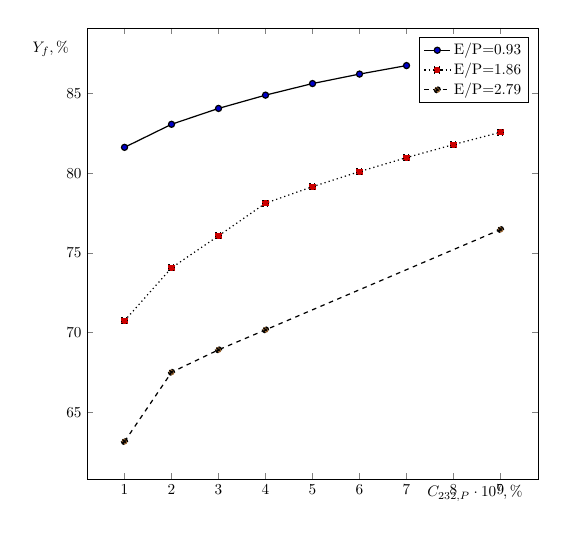
\begin{tikzpicture}[,
scale=0.55]
\begin{axis}[
  xlabel style = {{at={(axis description cs:.86,0)}}},
  ylabel = {$Y_{f}, \%$},
  ylabel style = {{at={(axis description cs:-0.08,.925)},rotate=270,anchor=south}},
  xlabel = {$C_{232,P}\cdot10^{7}, \%$},
  width=12cm, height=12cm
]

\addplot+[
  solid, black, thick
] coordinates {
  (1.0, 81.61991908264207)
  (2.0, 83.06585782673034)
  (3.0000000000000004, 84.06121871723813)
  (4.0, 84.89394884244733)
  (5.0, 85.62112811640561)
  (6.0, 86.21532750169558)
  (7.000000000000001, 86.74881397482362)
};
\addlegendentry{{}{E/P=0.93}}

\addplot+[
  dotted, black, thick
] coordinates {
  (1.0, 70.74596601492043)
  (2.0, 74.06158601844446)
  (3.0000000000000004, 76.06862560997918)
  (4.0, 78.11684252280332)
  (5.0, 79.15281009487043)
  (6.0, 80.09858956685858)
  (7.000000000000001, 80.97460907120315)
  (8.0, 81.7944538096466)
  (9.000000000000002, 82.56771088986454)
};
\addlegendentry{{}{E/P=1.86}}

\addplot+[
  dashed, black, thick
] coordinates {
  (1.0, 63.16381724872306)
  (2.0, 67.50888937364991)
  (3.0000000000000004, 68.91979697654483)
  (4.0, 70.1710975477616)
  (9.000000000000002, 76.46473227843333)
};
\addlegendentry{{}{E/P=2.79}}

\end{axis}
\end{tikzpicture}


\caption{{Зависимость степени извлечения $^{235}$U от ПДК $^{232}$U в НОУ-продукте с обогащением до уровня 5,5\% для различных $\frac{E}{P}$.{\label{ex55}}}}
\end{minipage}
\end{figure}

\begin{figure}
    \centering
    \begin{minipage}{.5\textwidth}
      \centering
      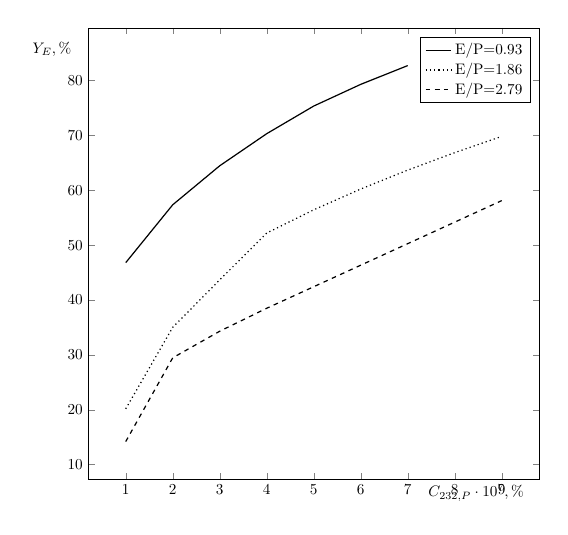
\begin{tikzpicture}[,
scale=0.55]
\begin{axis}[
  xlabel style = {{at={(axis description cs:.86,0)}}},
  ylabel = {$Y_{E}, \%$},
  ylabel style = {{at={(axis description cs:-0.08,.925)},rotate=270,anchor=south}},
  xlabel = {$C_{232,P}\cdot10^{7}, \%$},
  width=12cm, height=12cm
]

\addplot+[mark=none,
  solid, black, thick
] coordinates {
  (1.0, 46.800208774629716)
  (2.0, 57.35033934688334)
  (3.0000000000000004, 64.45948860219971)
  (4.0, 70.30908697025141)
  (5.0, 75.34542620989228)
  (6.0, 79.29919036071507)
  (7.000000000000001, 82.723141968642)
};
\addlegendentry{{}{E/P=0.93}}

\addplot+[mark=none,
  dotted, black, thick
] coordinates {
  (1.0, 20.160926232575846)
  (2.0, 35.007223506049215)
  (3.0000000000000004, 43.66597559028209)
  (4.0, 52.200316349986885)
  (5.0, 56.42853055286887)
  (6.0, 60.21940831661349)
  (7.000000000000001, 63.672842081572945)
  (8.0, 66.85533055225017)
  (9.000000000000002, 69.81385047110462)
};
\addlegendentry{{}{E/P=1.86}}

\addplot+[mark=none,
  dashed, black, thick
] coordinates {
  (1.0, 14.192755424067755)
  (2.0, 29.457231870306288)
  (3.0000000000000004, 34.301390009573225)
  (4.0, 38.492060382311266)
  (9.000000000000002, 58.11121612024639)
};
\addlegendentry{{}{E/P=2.79}}

\end{axis}
\end{tikzpicture}


\caption{{Зависимость степени извлечения $^{235}$U из регенерата от ПДК $^{232}$U в НОУ-продукте с обогащением до уровня 5,5\% для различных $\frac{E}{P}$.{\label{exR55}}}}
    \end{minipage}%
    \begin{minipage}{.5\textwidth}
      \centering
      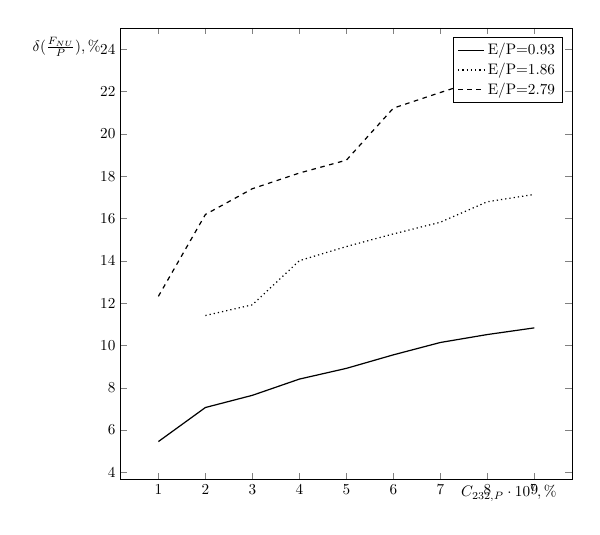
\begin{tikzpicture}[,
scale=0.55]
\begin{axis}[
  xlabel style = {{at={(axis description cs:.86,0)}}},
  ylabel = {$\delta(\frac{F_{NU}}{P}), \%$},
  ylabel style = {{at={(axis description cs:-0.12,.925)},rotate=270,anchor=south}},
  xlabel = {$C_{232,P}\cdot10^{7}, \%$},
  width=12cm, height=12cm
]

\addplot+[mark=none,
  solid, black, thick
] coordinates {
  (1.0, 5.4518852373011235)
  (2.0, 7.062106446811822)
  (3.0000000000000004, 7.6389396471428395)
  (4.0, 8.406580615825042)
  (5.0, 8.91372326597052)
  (6.0, 9.553487958028839)
  (7.000000000000001, 10.137926733330982)
  (8.0, 10.513552818081562)
  (9.000000000000002, 10.828975022060794)
};
\addlegendentry{{}{E/P=0.93}}

\addplot+[mark=none,
  dotted, black, thick
] coordinates {
  (2.0, 11.4125628071713)
  (3.0000000000000004, 11.919207344081862)
  (4.0, 14.00682887106841)
  (5.0, 14.67424564867117)
  (6.0, 15.272445794132029)
  (7.000000000000001, 15.824088637039257)
  (8.0, 16.793152631424558)
  (9.000000000000002, 17.14076317272052)
};
\addlegendentry{{}{E/P=1.86}}

\addplot+[mark=none,
  dashed, black, thick
] coordinates {
  (1.0, 12.320069331258377)
  (2.0, 16.18989448953321)
  (3.0000000000000004, 17.409881282949357)
  (4.0, 18.15088017430695)
  (5.0, 18.758892682933727)
  (6.0, 21.219879210414405)
  (7.000000000000001, 21.960274322729067)
  (8.0, 22.671364365359803)
  (9.000000000000002, 23.232704136321768)
};
\addlegendentry{{}{E/P=2.79}}

\end{axis}
\end{tikzpicture}


\caption{{Зависимость расхода природного урана от ПДК $^{232}$U в НОУ-продукте с обогащением до уровня 5,5\% для различных $\frac{E}{P}$.{\label{F0R55}}}}
\end{minipage}
\end{figure}







% \textbf{Сравнение интегральных параметров модифицированного двойного каскада с аналогичными параметрами для других способов обогащения регенерата урана. Дополнительные результаты.}



% Для демонстрации возможностей, получаемых применением предложенных в диссертации методик оптимизации, представим серию расчетов тройного каскада с НОУ-разбавителем, получив интегральные показатели для различных оптимизационных критериев.

% % РЕЗУЛЬТАТЫ СОМНИТЕЛЬНЫ - НЕ ЛУЧШЕ ДВОЙНОГО - ЗАНИМАЮСЬ АЛГОРИТМОМ

% \begin{table}
%     \begin{tabular}{ccccc}
%         $\cdot$ & $(Y_f)_\text{max}$ & $(Y_{E})_\text{max}$ & $(\delta(\frac{\Delta A}{P}))_\text{min}$ & $(\delta(\frac{F_{NU}}{P}))_\text{min}$\\ \hline
%         $\text{Сумм. степень изв-я}$ & $0.778$ & $0.07535$ & $0.07535$ & $0.03058$\\ \hline
%         $\text{Степень изв-я из рег-та}$ & $0.7976$ & $0.8765$ & $0.8765$ & $0.7504$\\ \hline
%         $\text{Потери РР, \%}$ & $6.814$ & $-1.127$ & $-1.127$ & $137.4$\\ \hline
%         $\text{Расх. пр. U на ед. прод.}$ & $6.217$ & $6.246$ & $6.246$ & $0.922$\\ \hline
%         $\text{Эк. пр. U, \%}$ & $21.62$ & $21.24$ & $21.24$ & $88.38$\\ \hline
%         $C_{235,P_1, \%}$ & $5.0$ & $5.0$ & $5.0$ & $15.0$\\ \hline
%         $C_{235,W_2, \%}$ & $4.227$ & $4.708$ & $4.708$ & $14.1$\\ \hline
%         $C_{235,P_0, \%}$ & $5.425$ & $5.321$ & $5.321$ & $5.456$\\ \hline
%         $C_{235,P_2, \%}$ & $16.0$ & $20.0$ & $20.0$ & $20.0$\\ \hline
%         $C_{232,P_1, \%}$ & $2.443e-6$ & $2.443e-6$ & $2.443e-6$ & $7.431e-6$\\ \hline
%         $C_{232,W_2, \%}$ & $1.515e-6$ & $1.998e-6$ & $1.998e-6$ & $6.329e-6$\\ \hline
%         $C_{232,P_2, \%}$ & $1.564e-5$ & $2.526e-5$ & $2.526e-5$ & $1.357e-5$\\ \hline
%         $C_{234,P_1, \%}$ & $0.1198$ & $0.1198$ & $0.1198$ & $0.3672$\\ \hline
%         $C_{234,W_2, \%}$ & $0.09223$ & $0.1084$ & $0.1084$ & $0.3349$\\ \hline
%         $C_{234,P_2, \%}$ & $0.512$ & $0.7049$ & $0.7049$ & $0.5472$\\ \hline
%         $C_{236,P_1, \%}$ & $2.942$ & $2.942$ & $2.942$ & $6.159$\\ \hline
%         $C_{236,W_2, \%}$ & $2.69$ & $2.856$ & $2.856$ & $5.955$\\ \hline
%         $\text{Уд. сумм. поток к-а 2}$ & $6.009$ & $2.627$ & $2.627$ & $0.2777$\\ \hline
%         $\text{Уд. сумм. поток доп. к-а}$ & $2285.0$ & $2285.0$ & $2285.0$ & $339.3$\\ \hline
%         $\text{Доля P2 в F3}$ & $0.002519$ & $1.0e-5$ & $1.0e-5$ & $1.0e-5$\\ \hline
%         $\text{U-235 в W3, \%}$ & $0.13$ & $0.13$ & $0.13$ & $0.1275$\\ \hline
%         $\text{U-235 в P3, \%}$ & $5.319$ & $4.617$ & $4.617$ & $4.253$\\ \hline
%         $\text{Р3, кг}$ & $74.86$ & $31.42$ & $31.42$ & $1219.0$\\ \hline
%         $\text{U-232, \%}$ & $5.0e-7$ & $4.945e-7$ & $4.945e-7$ & $4.552e-7$\\ \hline
%         $\text{U-234, \%}$ & $0.05795$ & $0.05973$ & $0.05973$ & $0.04356$\\ \hline
%         $\text{U-235, \%}$ & $5.137$ & $5.155$ & $5.155$ & $5.072$\\ \hline
%         $\text{U-236, \%}$ & $0.6463$ & $0.706$ & $0.706$ & $0.4194$\\ \hline
%         $F_{P_1}, \text{кг}$ & $372.8$ & $372.8$ & $372.8$ & $122.6$\\ \hline
%         $F_{W_2}, \text{кг}$ & $348.3$ & $365.6$ & $365.6$ & $103.9$\\ \hline
%         $F_{P_0}, \text{кг}$ & $1056.0$ & $1082.0$ & $1082.0$ & $155.7$\\ \hline
%         $F_{P_2}, \text{кг}$ & $24.48$ & $7.127$ & $7.127$ & $18.64$\\ \hline
%         \end{tabular}        
% \caption{Параметры схемы тройного каскада с НОУ-разбавителем при различных критериях оптимизации для обогащения регенерата второго рецикла.{\label{3opt2}}}
% \end{table}

% Анализируя результаты, представленные в \ref{3opt2}, заметим, что для оптимумов извлечения  $^{235}$U из регенерата и расхода работы разделения полученые решения идентичны. Эти решения позволяют вовлечь регенерат второго рецикла в ЯТЦ, оптимальным образом извлекая  $^{235}$U, выигрывая по этому показателю двойную схему, где $P_2$ не используется в производстве НОУ-продукта, не затрачивая дополнительную работу разделения по сравнению со схемой ординарного каскада для обогащения природного урана.
% Схема также позволяет найти решения, минимизирующие расход природного урана, в которых его затраты на единицу продукта будут на порядок меньше, однако это достигается за счет высокого расхода ОГФУ, и как следствие, больших потерь работы разделения (>100\%), а также ухудшения извлечения  $^{235}$U. 

% \begin{table}
%     \begin{tabular}{ccccc}
%         $\cdot$ & $(Y_f)_\text{max}$ & $(Y_{E})_\text{max}$ & $(\delta(\frac{\Delta A}{P}))_\text{min}$ & $(\delta(\frac{F_{NU}}{P}))_\text{min}$\\ \hline
%         $\text{Сумм. степень изв-я}$ & $0.7531$ & $0.04262$ & $0.7531$ & $0.02461$\\ \hline
%         $\text{Степень изв-я из рег-та}$ & $0.05408$ & $0.7628$ & $0.05408$ & $0.648$\\ \hline
%         $\text{Потери РР, \%}$ & $-0.4811$ & $11.38$ & $-0.4811$ & $173.3$\\ \hline
%         $\text{Расх. пр. U на ед. прод.}$ & $7.866$ & $6.882$ & $7.866$ & $0.2052$\\ \hline
%         $\text{Эк. пр. U, \%}$ & $0.8189$ & $13.23$ & $0.8189$ & $97.41$\\ \hline
%         $C_{235,P_1, \%}$ & $5.095$ & $5.0$ & $5.095$ & $9.0$\\ \hline
%         $C_{235,W_2, \%}$ & $4.923$ & $4.334$ & $4.923$ & $7.583$\\ \hline
%         $C_{235,P_0, \%}$ & $4.963$ & $5.428$ & $4.963$ & $4.736$\\ \hline
%         $C_{235,P_2, \%}$ & $16.0$ & $18.0$ & $16.0$ & $16.0$\\ \hline
%         $C_{232,P_1, \%}$ & $1.425e-5$ & $5.191e-6$ & $1.425e-5$ & $9.429e-6$\\ \hline
%         $C_{232,W_2, \%}$ & $1.257e-5$ & $2.852e-6$ & $1.257e-5$ & $5.601e-6$\\ \hline
%         $C_{232,P_2, \%}$ & $0.0001205$ & $5.087e-5$ & $0.0001205$ & $2.834e-5$\\ \hline
%         $C_{234,P_1, \%}$ & $0.2841$ & $0.1944$ & $0.2841$ & $0.3528$\\ \hline
%         $C_{234,W_2, \%}$ & $0.2681$ & $0.1507$ & $0.2681$ & $0.2694$\\ \hline
%         $C_{234,P_2, \%}$ & $1.295$ & $1.048$ & $1.295$ & $0.765$\\ \hline
%         $C_{236,P_1, \%}$ & $4.239$ & $5.446$ & $4.239$ & $9.226$\\ \hline
%         $C_{236,W_2, \%}$ & $4.167$ & $5.095$ & $4.167$ & $8.432$\\ \hline
%         $C_{236,P_2, \%}$ & $8.804$ & $12.3$ & $8.804$ & $13.14$\\ \hline
%         $M_{k1}$ & $234$ & $238$ & $234$ & $238$\\ \hline
%         $M_{k2}$ & $232$ & $232$ & $232$ & $232$\\ \hline
%         $\text{Уд. сумм. поток к-а 1}$ & $7.501$ & $371.5$ & $7.501$ & $441.2$\\ \hline
%         $\text{Уд. сумм. поток к-а 2}$ & $0.06838$ & $6.21$ & $0.06838$ & $1.869$\\ \hline
%         $\text{Уд. сумм. поток доп. к-а}$ & $2828.0$ & $2530.0$ & $2828.0$ & $72.87$\\ \hline
%         $\text{Доля P2 в F3}$ & $0.25$ & $1.0e-5$ & $0.25$ & $1.062e-5$\\ \hline
%         $\text{U-235 в W3, \%}$ & $0.105$ & $0.13$ & $0.105$ & $0.1275$\\ \hline
%         $\text{U-235 в P3, \%}$ & $4.896$ & $4.616$ & $4.896$ & $4.939$\\ \hline
%         $\text{Р3, кг}$ & $0.8097$ & $52.46$ & $0.8097$ & $1315.0$\\ \hline
%         $\text{U-232, \%}$ & $1.502e-7$ & $5.0e-7$ & $1.502e-7$ & $5.0e-7$\\ \hline
%         $\text{U-234, \%}$ & $0.04393$ & $0.06286$ & $0.04393$ & $0.04301$\\ \hline
%         $\text{U-235, \%}$ & $4.963$ & $5.208$ & $4.963$ & $5.156$\\ \hline
%         $\text{U-236, \%}$ & $0.04464$ & $0.89$ & $0.04464$ & $0.7112$\\ \hline
%         $F_{P_1}, \text{кг}$ & $15.59$ & $271.6$ & $15.59$ & $149.5$\\ \hline
%         $F_{W_2}, \text{кг}$ & $15.35$ & $258.4$ & $15.35$ & $124.4$\\ \hline
%         $F_{P_0}, \text{кг}$ & $1463.0$ & $1168.0$ & $1463.0$ & $40.04$\\ \hline
%         $F_{P_2}, \text{кг}$ & $0.2429$ & $13.23$ & $0.2429$ & $25.17$\\ \hline
%         \end{tabular}
% \caption{Параметры схемы тройного каскада с НОУ-разбавителем при различных критериях оптимизации для обогащения регенерата пятого рецикла.{\label{3opt5}}}
% \end{table}


% Анализируя результаты, представленные в \ref{3opt5}, заметим, что для оптимумов суммарной степени извлечения $^{235}$U из регенерата и расхода работы разделения полученые решения идентичны. Однако для них наблюдается низкая степень извлечения $^{235}$U из регенерата $\approx$5\%. При этом в решении с оптимумом извлечения $^{235}$U из регенерата, очень низка интегральная степень извлечения $^{235}$U  и составляет $\approx$5\%. 



% \begin{table}[h]
% \centering
% \begin{tabular}{ccc}
%     $\text{Каскад | П-р}$ & $\text{Уд. расход р-та}$ & $\text{ЕРР}$\\ \hline
%     $\text{С доп. питанием}$ & $0.01686$ & $11.82$\\ \hline
%     $\text{С доп. продуктом}$ & $0.07994$ & $11.95$\\ \hline
%     $\text{С доп. потоком питания}$ & $0.7552$ & $10.81$
% \end{tabular}\caption{{Параметры каскадов.{\label{table_ords}}}}
% \end{table}




% \begin{table}[h]
%     \centering
%     \begin{tabular}{|c|c|c|c|c|c|}
%     $\text{Каскад}$ & $\text{Экономия ЕРР,\%}$ & $\text{Уд.расход Регенерата,\%}$ & $\text{Уд.расход ОГФУ,\%}$ & $\text{Теор.стоимость,\%}$\\ \hline
%     1&7.31&1.04&0.49&0&92.71\\
%     2&100&41.63&8.26&0&0.32\\
%     3&10.07&6.08&0.93&0&89.96\\
%     4&15.08&25&0.93&31.11&85.00\\
%     4&23.13&50&0.93&74.49&77.02\\
%     \end{tabular}\caption{\label{from_splg19}Таблица сравнения каскадов.}
% \end{table}





% {'Cnp0': 0.16692258382642583, 'sw_loss': array([1.73328199]),
% 'isotope_composition_of_LEU_Product': {232: 4.999999999999999e-09, 233: 1.4111198357091083e-08, 234: 0.0005931559865097284, 235: 0.05167464967383427, 236: 0.007498791978738825, 238: 0.9402334023609172}, 'F0_to_LEU_Product': array([6.64739627]), 'P0_to_LEU_Product': array([0.24498671]), 'diluent_to_LEU_Product': array([0.75501329]), 'W0_to_LEU_Product': array([6.40240956]),
% 'Cip': {232: 0.0, 233: 0.0, 234: 0.001410328035664463, 235: 0.16692258382642994, 236: 0.0, 238: 0.8316670881379056},
% 'Ciw': {232: 0.0, 233: 0.0, 234: 2.100423399828056e-06, 235: 0.0009999999999999933, 236: 0.0, 238: 0.9989978995766002}, 'P_to_F': 0.036854536971271196, 'W_to_F': 0.9631454630287288, 'SumL_to_P': 11831.123257713576, 'SumL_to_W': 452.7151777696385, 'degree_of_235_involvement': array([0.8646317])}
% % 
% \setcounter{totalappendix}{\value{chapter}} % Подсчёт количества приложений

\end{document}